\documentclass[a4paper]{article}
\usepackage{vntex}
\usepackage{setspace}
\onehalfspacing
%\usepackage[english,vietnam]{babel}
%\usepackage[utf8]{inputenc}
\usepackage{mathptmx}[ptm]
%\usepackage[utf8]{inputenc}
%\usepackage[francais]{babel}
\usepackage{a4wide,amssymb,epsfig,latexsym,array,hhline,fancyhdr}
\usepackage[normalem]{ulem}
%\usepackage{soul}
\usepackage[table]{xcolor}
\usepackage[shortlabels]{enumitem}
\usepackage[makeroom]{cancel}
\usepackage{amsmath}
\usepackage{amsthm}
\usepackage{multicol,longtable,amscd}
\usepackage{diagbox}%Make diagonal lines in tables
\usepackage{booktabs}
\usepackage{alltt}
\usepackage[framemethod=tikz]{mdframed}% For highlighting paragraph backgrounds
\usepackage{caption,subcaption}


% \usepackage{lastpage} % Moved to after hyperref
\usepackage[lined,boxed,commentsnumbered]{algorithm2e}
% \usepackage{enumerate} % Removed in favor of enumitem with shortlabels
\usepackage{color}
\usepackage{graphicx}							% Standard graphics package
\usepackage{array}
\usepackage{tabularx, caption}
\usepackage{multirow}
\usepackage{multicol}
\usepackage{rotating}
\usepackage{graphics}
\usepackage{geometry}
\usepackage{setspace}
\usepackage{epsfig}
\usepackage{tikz}
\usepackage{float}
\usetikzlibrary{arrows,snakes,backgrounds,calc}
\usepackage[unicode]{hyperref}
\hypersetup{urlcolor=blue,linkcolor=black,citecolor=black,colorlinks=true} 
\usepackage{lastpage}
\usepackage{listings}

%\usepackage{pstcol} 								% PSTricks with the standard color package

\usepackage[normalem]{ulem}

\newtheorem{theorem}{{\bf Định lý}}
\newtheorem{property}{{\bf Tính chất}}
\newtheorem{proposition}{{\bf Mệnh đề}}
\newtheorem{corollary}[proposition]{{\bf Hệ quả}}
\newtheorem{lemma}[proposition]{{\bf Bổ đề}}
\theoremstyle{definition}
\newtheorem{exer}{Bài toán}
\addtocontents{toc}{\protect\thispagestyle{empty}}
% Remove page number in contents page. 
\addtocontents{lof}{\protect\thispagestyle{empty}}
% Remove page number in list of figure page. 
\addtocontents{lot}{\protect\thispagestyle{empty}}
% Remove page number in list of table page. 
\def\thesislayout{	% A4: 210 × 297
	\geometry{
		a4paper,
		total={160mm,240mm},  % fix over page
		left=30mm,
		top=22mm,
            right=20mm,
            bottom=20mm,
	}
}
\def\thesisheadlayout{	% A4: 210 × 297
	\geometry{
		a4paper,
		total={160mm,240mm},  % fix over page
		left=30mm,
		top=10mm,
	}
}
\thesislayout
\lstset{
language=R,
basicstyle=\footnotesize\sffamily,
commentstyle=\ttfamily\color{black},
numbers=left,
numberstyle=\ttfamily\color{black}\footnotesize,
stepnumber=1,
numbersep=5pt,
backgroundcolor=\color{white},
showspaces=false,
showstringspaces=false,
showtabs=false,
frame=single,
tabsize=2,
captionpos=b,
breaklines=true,
breakatwhitespace=false,
title=\lstname,
escapeinside={},
keywordstyle={},
morekeywords={}
}
%\usepackage{fancyhdr}
\setlength{\headheight}{40pt}
\pagestyle{fancy}
\fancyhead{} % clear all header fields
\renewcommand{\footruleskip}{1mm}

\fancyhead[L]{
 \begin{tabular}{rl}
    \begin{picture}(25,15)(0,0)
    \put(0,-8){
\includegraphics[width=10mm, height=10mm]{Images/hcmut.png}}
    %\put(0,-8){
\epsfig{width=10mm,figure=hcmut.eps}}
   \end{picture}&
	%
\includegraphics[width=8mm, height=8mm]{hcmut.png} & %
	\begin{tabular}{l}
		\textbf{  Trường Đại Học Bách Khoa - Đại học Quốc gia TP.HCM }\\
		\textbf{  Khoa Khoa Học \& Kỹ Thuật Máy Tính}
	\end{tabular} 	
 \end{tabular}
}
\fancyhead[R]{
	\begin{tabular}{l}
		\tiny \bf \\
		\tiny \bf 
	\end{tabular}  }
\fancyfoot{} % clear all footer fields
\fancyfoot[L]{\scriptsize  Báo cáo Đồ án chuyên ngành - HK1 2025 - 2026}
\fancyfoot[R]{\scriptsize  Trang {\thepage}/\pageref{LastPage}}

\renewcommand{\headrulewidth}{0.3pt}
\renewcommand{\footrulewidth}{0.3pt}

%%%
\setcounter{secnumdepth}{4}
\setcounter{tocdepth}{3}
\makeatletter
\newcounter {subsubsubsection}[subsubsection]
\renewcommand\thesubsubsubsection{\thesubsubsection .\@alph\c@subsubsubsection}
\newcommand\subsubsubsection{\@startsection{subsubsubsection}{4}{\z@}%
                                     {-3.25ex\@plus -1ex \@minus -.2ex}%
                                     {1.5ex \@plus .2ex}%
                                     {\normalfont\normalsize\bfseries}}
\newcommand*\l@subsubsubsection{\@dottedtocline{3}{10.0em}{4.1em}}
\newcommand*{\subsubsubsectionmark}[1]{}
\makeatother

\everymath{\color{black}}%make in-line maths symbols blue to read/check easily

\sloppy
\captionsetup[figure]{labelfont={small,bf},textfont={small,it},belowskip=-1pt,aboveskip=-9pt}
%space remove between caption, figure, and text
\captionsetup[table]{labelfont={small,bf},textfont={small,it},belowskip=-1pt,aboveskip=7pt}
\setlength{\floatsep}{5pt plus 2pt minus 2pt}
\setlength{\textfloatsep}{5pt plus 2pt minus 2pt}
\setlength{\intextsep}{10pt plus 2pt minus 2pt}

\thesislayout

\begin{document}

\begin{titlepage}
\begin{tikzpicture}[remember picture, overlay]
  \draw[line width = 4pt] ($(current page.north west) + (0.4in,-0.5in)$) rectangle ($(current page.south east) + (-0.4in,0.5in)$);
  \draw[line width=1.5pt]
    ($ (current page.north west) + (0.45in,-0.55in) $)
    rectangle
    ($ (current page.south east) + (-0.45in,0.55in) $);
\end{tikzpicture}

\begin{center}
\LARGE \textbf{ĐẠI HỌC QUỐC GIA THÀNH PHỐ HỒ CHÍ MINH} \\
\vspace{0.2cm}
\LARGE \textbf{TRƯỜNG ĐẠI HỌC BÁCH KHOA} \\
\vspace{0.2cm}
\LARGE \textbf{KHOA KHOA HỌC VÀ KĨ THUẬT MÁY TÍNH}
\end{center}

\vspace{0.3cm}

\begin{figure}[h!]
\begin{center}

\includegraphics[width=4cm]{Images/hcmut.png}
\end{center}
\end{figure}

\begin{center}
\begin{tabular}{c}
    % Phần tiêu đề báo cáo
    \textbf{\LARGE BÁO CÁO} \\
    \vspace{0.05cm} \\ % Khoảng cách nhỏ
    \textbf{\LARGE ĐỒ ÁN CHUYÊN NGÀNH} \\
    \vspace{0.5cm} \\

    % Phần tên đề tài: Sử dụng parbox để tự động xuống dòng
    % 12cm là chiều rộng tối đa của tên đề tài (bạn có thể thay đổi số này)
    \parbox{12cm}{
        \centering \LARGE \textbf{MÔ HÌNH KHO DỮ LIỆU (DATA WAREHOUSE) VỀ GIAO THÔNG PHỤC VỤ CÔNG TÁC THỐNG KÊ, DỰ BÁO, HỖ TRỢ RA QUYẾT ĐỊNH}
    } \\
    
    \vspace{0.2cm} \\
    
    {\Large NGÀNH: KHOA HỌC MÁY TÍNH}
\end{tabular}
\end{center}
\vspace{0.5cm}
\begin{table}[h]
\begin{tabular}{rll}
\hspace{6 cm} &  \textbf{\Large CBHD1:} {\Large PGS.TS. Trần Minh Quang}
\\
\\
\hspace{6 cm} &   \textbf{\Large CBHD2:} {\Large ThS. Bùi Tiến Đức}
\\
\\


\\
\hspace{6 cm} &   \textbf{\Large SVTH1:} {\Large Đinh Nguyễn Việt Khiêm (2211565)}
\\
\\
\hspace{6 cm}&   \textbf{\Large SVTH2:}  {\Large Nguyễn Thành Dũng (2210589)}
\\
\\
\hspace{6 cm} &   \textbf{\Large SVTH3:}  {\Large Hồ Trần Ngọc Liêm (2211835)}
\\
\\
\end{tabular}
\end{table}
\vspace{0.5cm}
\begin{center}
{\Large TP. HỒ CHÍ MINH, THÁNG 12 NĂM 2025 }
\end{center}
\end{titlepage}
%\thispagestyle{empty}
\newpage
%%%%%%%%%%%%%%%%%INTRO%%%%%%%%%%%%%%%%%%%
% % \input{Intro/LoiCamOn}
% % \input{Intro/LoiCamDoan}
% % \input{Intro/TomTat}
\newpage
\tableofcontents
\newpage

% --- Danh mục hình ảnh ---
\cleardoublepage
\phantomsection
\addcontentsline{toc}{section}{Danh mục hình ảnh} % Thêm dòng này để hiện tên mục này trong Mục lục
\listoffigures 
\newpage

% --- Danh mục bảng biểu ---
\cleardoublepage
\phantomsection
\addcontentsline{toc}{section}{Danh mục bảng biểu} % Thêm dòng này để hiện tên mục này trong Mục lục
\listoftables
\newpage

% \listoffigures
% \newpage
% \listoftables
% \newpage
% \setcounter{page}{1}

%%%%%%%%%%%%%%%%%CONTENTS%%%%%%%%%%%%%%%%%%%
\section{Giới thiệu}
\subsection{Động cơ của đề tài}

Trong bối cảnh tốc độ đô thị hóa và gia tăng dân số diễn ra mạnh mẽ trong nhiều năm gần đây, Thành phố Hồ Chí Minh (TP.HCM) đang phải đối mặt với những áp lực ngày càng lớn đối với hệ thống giao thông đô thị. Sự gia tăng nhanh chóng của phương tiện cá nhân, đặc biệt là xe máy và ô tô, trong khi năng lực hạ tầng giao thông chưa theo kịp tốc độ phát triển đô thị, đã dẫn đến tình trạng ùn tắc giao thông diễn ra thường xuyên tại nhiều tuyến đường và khu vực trọng điểm. Thực trạng này không chỉ làm suy giảm hiệu quả vận hành của đô thị mà còn gây ra nhiều hệ lụy nghiêm trọng như ô nhiễm môi trường, gia tăng thời gian di chuyển, tiêu hao năng lượng, tai nạn giao thông và ảnh hưởng trực tiếp đến chất lượng sống của người dân.

Trước yêu cầu phát triển đô thị bền vững, TP.HCM đã định hướng xây dựng mô hình đô thị thông minh, trong đó giao thông thông minh (Intelligent Transportation System – ITS) được xem là một trong những lĩnh vực ưu tiên trọng điểm. Tuy nhiên, phần lớn các hệ thống giám sát và quản lý giao thông hiện nay mới chỉ tập trung vào chức năng quan sát và phản ứng theo thời gian thực, trong khi còn thiếu một nền tảng dữ liệu tập trung có khả năng tích hợp, lưu trữ và phân tích dữ liệu giao thông trên quy mô lớn và dài hạn. Điều này làm hạn chế khả năng khai thác dữ liệu phục vụ công tác thống kê, đánh giá xu hướng, tối ưu hóa vận hành và hỗ trợ ra quyết định chiến lược.

Hiện nay, dữ liệu giao thông đô thị được hình thành từ nhiều nguồn dị biệt như hệ thống camera giám sát (CCTV), thiết bị định vị GPS, dữ liệu cảm biến giao thông, nền tảng bản đồ số, cũng như dữ liệu lưu lượng và sự cố được cung cấp từ các nền tảng giao thông trực tuyến. Các nguồn dữ liệu này có đặc trưng phân tán, không đồng nhất về cấu trúc và thiếu tính liên kết không gian – thời gian, dẫn đến khó khăn trong việc đồng bộ, tổng hợp và khai thác phân tích chuyên sâu. Đặc biệt, đối với các bài toán giao thông thông minh hiện đại, dữ liệu không gian địa lý (geospatial data) đóng vai trò then chốt trong việc mô hình hóa mạng lưới giao thông, xác định các tuyến trọng điểm, phân tích mật độ lưu thông và đánh giá mức độ ùn tắc theo từng khu vực.

Trong bối cảnh đó, mô hình kho dữ liệu giao thông (Traffic Data Warehouse) kết hợp với công nghệ dữ liệu không gian (Spatial Data Warehouse) được xem là giải pháp nền tảng nhằm giải quyết bài toán phân mảnh dữ liệu. Kho dữ liệu cho phép tích hợp dữ liệu từ nhiều nguồn khác nhau, chuẩn hóa và tổ chức dữ liệu theo cấu trúc đa chiều, hỗ trợ hiệu quả cho các truy vấn phân tích phức tạp, thống kê lịch sử và khai thác dữ liệu quy mô lớn. Khác với các hệ quản trị cơ sở dữ liệu giao dịch truyền thống (OLTP), kho dữ liệu được tối ưu hóa cho các tác vụ phân tích (OLAP), đặc biệt phù hợp với các bài toán xử lý dữ liệu giao thông theo chiều không gian – thời gian và phục vụ công tác điều hành đô thị thông minh.

Bên cạnh đó, sự phát triển mạnh mẽ của trí tuệ nhân tạo (Artificial Intelligence – AI) và học máy (Machine Learning) đang thúc đẩy quá trình chuyển đổi từ mô hình quản lý giao thông mang tính phản ứng (reactive traffic management) sang mô hình quản lý chủ động và dự báo (proactive traffic management). Các mô hình AI có khả năng phân tích xu hướng lưu lượng, dự báo nguy cơ ùn tắc và hỗ trợ tối ưu hóa điều phối giao thông theo thời gian thực. Tuy nhiên, hiệu quả của các mô hình dự báo phụ thuộc rất lớn vào chất lượng dữ liệu đầu vào, đòi hỏi một hạ tầng dữ liệu đủ lớn, ổn định, được chuẩn hóa và cập nhật liên tục. Đây chính là vai trò cốt lõi của hệ thống kho dữ liệu giao thông tích hợp.

Xuất phát từ những yêu cầu thực tiễn nêu trên, nhóm nghiên cứu quyết định thực hiện đề tài: “Mô hình kho dữ liệu giao thông phục vụ công tác thống kê, phân tích và dự báo hỗ trợ điều hành giao thông thông minh”. Đề tài tập trung xây dựng một nền tảng dữ liệu giao thông tích hợp trên cơ sở kết hợp dữ liệu thời gian thực từ các nguồn giao thông trực tuyến với dữ liệu không gian địa lý, triển khai quy trình ETL tự động nhằm thu thập, làm sạch, biến đổi và lưu trữ dữ liệu trong kho dữ liệu không gian. Đồng thời, hệ thống hướng đến việc ứng dụng các mô hình trí tuệ nhân tạo trong phân tích và dự báo tình trạng giao thông, kết hợp với nền tảng trực quan hóa và dashboard hỗ trợ giám sát, từ đó góp phần xây dựng nền tảng hạ tầng dữ liệu phục vụ phát triển hệ sinh thái giao thông thông minh và đô thị thông minh tại TP.HCM trong tương lai.


\subsection{Mục tiêu}

Mục tiêu tổng quát của đề tài là nghiên cứu, thiết kế và triển khai một nền tảng kho dữ liệu giao thông thông minh có khả năng tích hợp dữ liệu đa nguồn, xử lý dữ liệu không gian – thời gian theo thời gian thực và hỗ trợ các tác vụ phân tích, dự báo phục vụ công tác quản lý và điều hành giao thông đô thị. Hệ thống được định hướng xây dựng theo mô hình kiến trúc dữ liệu hiện đại, bảo đảm khả năng mở rộng, tính ổn định và đáp ứng yêu cầu khai thác dữ liệu quy mô lớn trong bối cảnh phát triển đô thị thông minh.

Để hiện thực hóa mục tiêu tổng quát nêu trên, đề tài tập trung vào các mục tiêu cụ thể sau:

\begin{itemize}

    \item \textbf{Nghiên cứu và đề xuất kiến trúc kho dữ liệu giao thông thông minh}\\
    Xây dựng kiến trúc tổng thể cho hệ thống kho dữ liệu giao thông theo mô hình đa tầng, bao gồm tầng thu thập dữ liệu, tầng lưu trữ dữ liệu không gian, tầng phân tích trí tuệ nhân tạo và tầng trực quan hóa dữ liệu. Đề tài tập trung thiết kế mô hình dữ liệu đa chiều phù hợp với đặc thù dữ liệu giao thông đô thị tại Việt Nam, kết hợp giữa dữ liệu cấu trúc, bán cấu trúc và dữ liệu không gian địa lý (geospatial data). Các mô hình Star Schema hoặc Snowflake Schema được nghiên cứu và áp dụng nhằm tối ưu hóa hiệu năng truy vấn, hỗ trợ hiệu quả cho các tác vụ phân tích dữ liệu lớn và xử lý theo chiều không gian – thời gian.

    \item \textbf{Xây dựng quy trình xử lý dữ liệu ETL/ELT tự động}\\
    Thiết kế và triển khai quy trình ETL/ELT nhằm tự động hóa quá trình thu thập, biến đổi và lưu trữ dữ liệu giao thông từ nhiều nguồn khác nhau như API giao thông thời gian thực, dữ liệu bản đồ số OpenStreetMap (OSM), dữ liệu sự cố giao thông và các nguồn dữ liệu hỗ trợ khác. Quy trình xử lý dữ liệu tập trung vào việc làm sạch dữ liệu, xử lý ngoại lệ, chuẩn hóa định dạng, tích hợp dữ liệu không gian và tối ưu khả năng cập nhật dữ liệu liên tục theo chu kỳ thời gian thực, bảo đảm tính toàn vẹn và độ tin cậy của dữ liệu trong kho dữ liệu trung tâm.

    \item \textbf{Xây dựng kho dữ liệu không gian phục vụ phân tích giao thông}\\
    Triển khai hệ quản trị cơ sở dữ liệu PostgreSQL kết hợp với phần mở rộng PostGIS nhằm hỗ trợ lưu trữ và xử lý dữ liệu không gian địa lý. Đề tài tập trung xây dựng mô hình dữ liệu phục vụ quản lý các thực thể giao thông như tuyến đường, đoạn đường, nút giao, vùng ảnh hưởng và dữ liệu lưu lượng theo không gian – thời gian. Đồng thời, hệ thống được tối ưu hóa nhằm đáp ứng các truy vấn phân tích không gian phức tạp và hỗ trợ trực quan hóa dữ liệu giao thông trên nền bản đồ số.

    \item \textbf{Tích hợp và triển khai mô hình trí tuệ nhân tạo phục vụ dự báo giao thông}\\
    Nghiên cứu và ứng dụng các mô hình học máy và học sâu trong bài toán dự báo tình trạng giao thông đô thị, bao gồm dự báo lưu lượng phương tiện, tốc độ lưu thông và nguy cơ ùn tắc. Các mô hình như ARIMA, LSTM hoặc các mô hình lai ghép (Hybrid Models) được huấn luyện và đánh giá trên tập dữ liệu lịch sử đã được chuẩn hóa từ kho dữ liệu giao thông. Quá trình huấn luyện và kiểm thử mô hình được thực hiện theo quy trình khoa học nhằm bảo đảm độ chính xác và khả năng ứng dụng thực tiễn của hệ thống dự báo.

    \item \textbf{Phát triển hệ thống trực quan hóa và hỗ trợ ra quyết định}\\
    Xây dựng nền tảng dashboard và web application phục vụ giám sát giao thông theo thời gian thực, hỗ trợ trực quan hóa dữ liệu dưới dạng biểu đồ, bản đồ nhiệt (heatmap), thống kê lưu lượng và cảnh báo ùn tắc. Hệ thống hướng đến việc cung cấp công cụ hỗ trợ ra quyết định cho các cơ quan quản lý giao thông đô thị, hỗ trợ công tác điều phối giao thông, phân luồng phương tiện và hoạch định chính sách phát triển hạ tầng giao thông thông minh.

    \item \textbf{Triển khai thử nghiệm và đánh giá hiệu năng hệ thống}\\
    Tiến hành triển khai thử nghiệm hệ thống trên hạ tầng điện toán đám mây Microsoft Azure, kết hợp với nền tảng container hóa Docker nhằm bảo đảm tính linh hoạt và khả năng mở rộng của hệ thống. Đề tài thực hiện đánh giá hiệu năng của quy trình xử lý dữ liệu thời gian thực, khả năng đáp ứng của kho dữ liệu, mức độ ổn định của hệ thống cũng như độ chính xác của mô hình dự báo trên dữ liệu thực tế. Các kết quả đánh giá được sử dụng làm cơ sở để phân tích tính khả thi và khả năng ứng dụng của hệ thống trong bài toán giao thông thông minh tại TP.HCM.

\end{itemize}

\subsection{Phạm vi}

Nhằm bảo đảm tính khả thi của đề tài trong điều kiện thời gian, nguồn lực và phạm vi nghiên cứu, hệ thống được giới hạn trong các nội dung nghiên cứu và triển khai cụ thể như sau:

\begin{itemize}

    \item \textbf{Về dữ liệu nghiên cứu}\\
    Đề tài tập trung khai thác và xử lý các loại dữ liệu giao thông có cấu trúc và bán cấu trúc phục vụ cho bài toán phân tích giao thông thông minh. Các nguồn dữ liệu chính bao gồm dữ liệu lưu lượng giao thông thời gian thực, dữ liệu tốc độ lưu thông, dữ liệu sự cố giao thông, dữ liệu định vị GPS và dữ liệu bản đồ số từ nền tảng OpenStreetMap (OSM). Ngoài ra, hệ thống có khả năng mở rộng để tích hợp dữ liệu từ các cảm biến IoT hoặc nền tảng giám sát giao thông trong tương lai. Đối với dữ liệu phi cấu trúc như video thô từ camera CCTV, đề tài không thực hiện xử lý trực tiếp mà chỉ sử dụng các dữ liệu đã được trích xuất và chuyển đổi sang dạng số liệu phục vụ phân tích.

    \item \textbf{Về phạm vi không gian nghiên cứu}\\
    Hệ thống được triển khai thử nghiệm và đánh giá trên một số tuyến đường trọng điểm, các hành lang giao thông chính và các khu vực có mật độ lưu thông cao tại Thành phố Hồ Chí Minh. Phạm vi nghiên cứu tập trung vào các tuyến đường thường xuyên xảy ra ùn tắc giao thông nhằm phục vụ việc phân tích lưu lượng, đánh giá mức độ quá tải và thử nghiệm khả năng dự báo tình trạng giao thông theo thời gian thực. Kết quả thử nghiệm được sử dụng làm cơ sở đánh giá tính khả thi và khả năng mở rộng của mô hình trong quy mô đô thị lớn.

    \item \textbf{Về phạm vi công nghệ và hạ tầng triển khai}\\
    Đề tài sử dụng hệ quản trị cơ sở dữ liệu PostgreSQL kết hợp với phần mở rộng PostGIS để xây dựng kho dữ liệu không gian phục vụ lưu trữ và xử lý dữ liệu giao thông. Quy trình ETL/ELT được phát triển bằng ngôn ngữ Python kết hợp với các thư viện hỗ trợ xử lý dữ liệu và kết nối cơ sở dữ liệu như SQLAlchemy, GeoAlchemy2 và Pandas. Hệ thống được triển khai trên nền tảng điện toán đám mây Microsoft Azure, sử dụng Docker và Docker Compose để quản lý môi trường thực thi và hỗ trợ khả năng mở rộng hệ thống. Các mô hình trí tuệ nhân tạo và học máy được xây dựng và huấn luyện thông qua các thư viện khoa học dữ liệu như Scikit-learn, TensorFlow hoặc PyTorch.

    \item \textbf{Về phạm vi chức năng hệ thống}\\
    Đề tài tập trung nghiên cứu và phát triển nền tảng phần mềm phục vụ thu thập, xử lý, lưu trữ, phân tích và trực quan hóa dữ liệu giao thông. Hệ thống hỗ trợ xây dựng dashboard giám sát giao thông, phân tích dữ liệu lịch sử và tích hợp mô hình dự báo tình trạng ùn tắc giao thông theo thời gian thực. Đề tài không bao gồm việc thiết kế hoặc triển khai hạ tầng phần cứng vật lý như camera giao thông, thiết bị IoT hoặc hệ thống cảm biến ngoài thực địa. Các nguồn dữ liệu đầu vào được giả định là có sẵn thông qua API, dữ liệu mở hoặc các nền tảng hỗ trợ nghiên cứu.

    \item \textbf{Về phạm vi nghiên cứu mô hình dự báo}\\
    Đề tài tập trung vào các bài toán dự báo ngắn hạn liên quan đến lưu lượng giao thông, tốc độ lưu thông và nguy cơ ùn tắc trên từng tuyến đường hoặc khu vực cụ thể. Các mô hình học máy và học sâu được xây dựng nhằm đánh giá khả năng ứng dụng của trí tuệ nhân tạo trong hỗ trợ điều hành giao thông thông minh, tuy nhiên chưa đi sâu vào các bài toán tối ưu điều khiển tín hiệu giao thông hoặc điều phối giao thông quy mô toàn thành phố.

\end{itemize}

\subsection{Ý nghĩa}

\subsubsection{Ý nghĩa thực tiễn}

Đề tài mang ý nghĩa thực tiễn quan trọng trong bối cảnh nhu cầu xây dựng hệ thống giao thông thông minh và đô thị thông minh tại Thành phố Hồ Chí Minh ngày càng trở nên cấp thiết. Việc xây dựng nền tảng kho dữ liệu giao thông tích hợp không chỉ góp phần nâng cao hiệu quả quản lý dữ liệu mà còn tạo tiền đề cho việc ứng dụng các công nghệ phân tích dữ liệu lớn và trí tuệ nhân tạo trong công tác điều hành giao thông đô thị.

\begin{itemize}

    \item \textbf{Hỗ trợ công tác quản lý và điều hành giao thông đô thị}\\
    Hệ thống kho dữ liệu giao thông cho phép tập trung, chuẩn hóa và lưu trữ dữ liệu từ nhiều nguồn khác nhau trong một nền tảng thống nhất, giúp các cơ quan quản lý như Sở Giao thông Vận tải Thành phố Hồ Chí Minh có được cái nhìn toàn diện về hiện trạng giao thông theo không gian và thời gian. Thông qua hệ thống dashboard và các công cụ trực quan hóa dữ liệu, nhà quản lý có thể theo dõi lưu lượng giao thông theo thời gian thực, đánh giá mức độ ùn tắc tại các khu vực trọng điểm và hỗ trợ ra quyết định trong công tác phân luồng, điều phối giao thông cũng như hoạch định chính sách phát triển hạ tầng.

    \item \textbf{Nâng cao hiệu quả khai thác và sử dụng dữ liệu giao thông}\\
    Việc xây dựng quy trình ETL/ELT tự động và kho dữ liệu không gian giúp giải quyết tình trạng dữ liệu giao thông phân tán, thiếu đồng bộ và khó khai thác. Hệ thống cho phép lưu trữ dữ liệu lịch sử với quy mô lớn, hỗ trợ các tác vụ thống kê, phân tích xu hướng và truy vấn dữ liệu phức tạp, từ đó nâng cao hiệu quả sử dụng dữ liệu phục vụ nghiên cứu và vận hành thực tiễn.

    \item \textbf{Hỗ trợ dự báo và giảm thiểu ùn tắc giao thông}\\
    Việc tích hợp các mô hình trí tuệ nhân tạo và học máy vào hệ thống cho phép dự báo lưu lượng phương tiện, tốc độ lưu thông và nguy cơ ùn tắc trong tương lai gần. Các kết quả dự báo có thể hỗ trợ cơ quan quản lý chủ động trong công tác điều tiết giao thông, bố trí lực lượng chức năng hợp lý và đưa ra các giải pháp ứng phó kịp thời nhằm giảm thiểu tác động tiêu cực của ùn tắc giao thông đối với đời sống đô thị.

    \item \textbf{Tạo nền tảng cho phát triển hệ sinh thái giao thông thông minh}\\
    Hệ thống được thiết kế theo hướng kiến trúc mở và có khả năng mở rộng linh hoạt, cho phép tích hợp thêm nhiều nguồn dữ liệu và dịch vụ thông minh khác trong tương lai như dữ liệu IoT, camera giao thông, dữ liệu thời tiết hoặc các nền tảng giao thông công cộng. Điều này góp phần hình thành nền tảng hạ tầng dữ liệu phục vụ phát triển hệ sinh thái giao thông thông minh và đô thị thông minh tại Việt Nam.

    \item \textbf{Khả năng ứng dụng và mở rộng thực tiễn}\\
    Mô hình hệ thống được triển khai trên nền tảng điện toán đám mây và sử dụng các công nghệ mã nguồn mở phổ biến, qua đó bảo đảm tính linh hoạt, khả năng mở rộng và tối ưu chi phí triển khai. Kết quả nghiên cứu có thể được sử dụng làm cơ sở tham khảo cho các bài toán quản lý giao thông tại các đô thị lớn khác ở Việt Nam.

\end{itemize}

\subsubsection{Ý nghĩa khoa học}

Bên cạnh giá trị thực tiễn, đề tài còn mang ý nghĩa khoa học trong lĩnh vực dữ liệu lớn, hệ thống thông tin địa lý và trí tuệ nhân tạo ứng dụng trong giao thông thông minh.

\begin{itemize}

    \item \textbf{Đóng góp về mô hình hóa dữ liệu giao thông không gian – thời gian}\\
    Đề tài nghiên cứu và xây dựng mô hình kho dữ liệu giao thông theo hướng tích hợp dữ liệu không gian – thời gian (spatio-temporal data warehouse), kết hợp giữa dữ liệu giao thông thời gian thực và dữ liệu địa lý không gian. Việc áp dụng các mô hình dữ liệu đa chiều trong bối cảnh dữ liệu giao thông tại Việt Nam góp phần kiểm chứng tính khả thi của phương pháp tiếp cận này đối với các bài toán phân tích giao thông đô thị.

    \item \textbf{Đóng góp trong lĩnh vực xử lý và tích hợp dữ liệu giao thông đa nguồn}\\
    Nghiên cứu đề xuất quy trình ETL/ELT phục vụ thu thập, làm sạch, chuẩn hóa và tích hợp dữ liệu từ nhiều nguồn dị biệt khác nhau. Đây là cơ sở quan trọng cho việc xây dựng các hệ thống dữ liệu giao thông có khả năng xử lý dữ liệu lớn, dữ liệu thời gian thực và dữ liệu không gian trong môi trường đô thị thông minh.

    \item \textbf{Đánh giá khả năng ứng dụng trí tuệ nhân tạo trong dự báo giao thông}\\
    Đề tài thực hiện thử nghiệm các mô hình học máy và học sâu trên dữ liệu giao thông thực tế nhằm đánh giá hiệu quả dự báo lưu lượng và tình trạng ùn tắc giao thông. Kết quả nghiên cứu góp phần bổ sung cơ sở thực nghiệm cho việc ứng dụng trí tuệ nhân tạo trong lĩnh vực giao thông thông minh tại Việt Nam, đặc biệt trong bối cảnh giao thông hỗn hợp và có mật độ phương tiện cao.

    \item \textbf{Đóng góp về kiến trúc hệ thống dữ liệu giao thông thông minh}\\
    Kiến trúc hệ thống được xây dựng theo mô hình phân tầng bao gồm tầng thu thập dữ liệu, tầng kho dữ liệu không gian, tầng trí tuệ nhân tạo và tầng trực quan hóa. Mô hình này có thể được xem như một hướng tiếp cận tham khảo cho việc phát triển các nền tảng Traffic Integrated Operations Center (Traffic IOC) hoặc các hệ thống phân tích giao thông thông minh trong tương lai.

\end{itemize}

\subsection{Đóng góp của đề tài}

Đề tài hướng đến việc xây dựng một nền tảng dữ liệu giao thông thông minh tích hợp nhiều thành phần công nghệ hiện đại, bao gồm kho dữ liệu không gian, xử lý dữ liệu thời gian thực, trí tuệ nhân tạo và hệ thống trực quan hóa phục vụ quản lý giao thông đô thị. Trên cơ sở đó, các đóng góp chính của đề tài được xác định như sau:

\begin{itemize}

    \item \textbf{Đề xuất mô hình kho dữ liệu giao thông tích hợp dữ liệu không gian – thời gian}\\
    Đề tài xây dựng mô hình kho dữ liệu giao thông theo hướng tích hợp dữ liệu đa nguồn kết hợp với dữ liệu địa lý không gian (geospatial data). Mô hình dữ liệu được thiết kế nhằm hỗ trợ lưu trữ, quản lý và phân tích dữ liệu giao thông theo cả hai chiều không gian và thời gian, phục vụ hiệu quả cho các bài toán thống kê, phân tích lưu lượng và dự báo giao thông trong môi trường đô thị thông minh.

    \item \textbf{Xây dựng quy trình ETL/ELT tự động cho dữ liệu giao thông thời gian thực}\\
    Đề tài triển khai quy trình thu thập, xử lý và đồng bộ dữ liệu giao thông theo thời gian thực từ nhiều nguồn dữ liệu khác nhau thông qua API và dữ liệu bản đồ số. Quy trình ETL/ELT được tối ưu nhằm bảo đảm khả năng xử lý dữ liệu liên tục, tự động hóa việc làm sạch dữ liệu, xử lý ngoại lệ và chuẩn hóa dữ liệu trước khi lưu trữ vào kho dữ liệu trung tâm.

    \item \textbf{Ứng dụng công nghệ cơ sở dữ liệu không gian trong quản lý giao thông}\\
    Đề tài khai thác khả năng của PostgreSQL kết hợp với PostGIS để xây dựng kho dữ liệu không gian phục vụ lưu trữ và xử lý các thực thể giao thông như tuyến đường, đoạn đường, nút giao và dữ liệu lưu lượng theo vị trí địa lý. Việc ứng dụng công nghệ dữ liệu không gian góp phần nâng cao khả năng phân tích giao thông theo khu vực và hỗ trợ trực quan hóa dữ liệu trên nền bản đồ số.

    \item \textbf{Tích hợp mô hình trí tuệ nhân tạo phục vụ dự báo giao thông}\\
    Đề tài nghiên cứu và triển khai các mô hình học máy và học sâu nhằm dự báo tình trạng giao thông trong ngắn hạn, bao gồm dự báo lưu lượng phương tiện, tốc độ lưu thông và nguy cơ ùn tắc. Các mô hình được huấn luyện và đánh giá trên tập dữ liệu thực tế đã được xử lý và chuẩn hóa từ kho dữ liệu giao thông, qua đó kiểm chứng khả năng ứng dụng của trí tuệ nhân tạo trong bài toán giao thông đô thị tại Việt Nam.

    \item \textbf{Xây dựng hệ thống trực quan hóa và hỗ trợ ra quyết định}\\
    Đề tài phát triển nền tảng dashboard và web application phục vụ giám sát giao thông theo thời gian thực, hỗ trợ trực quan hóa dữ liệu dưới dạng biểu đồ, bản đồ nhiệt và thống kê lưu lượng giao thông. Hệ thống góp phần hỗ trợ cơ quan quản lý trong công tác điều hành, phân luồng và đánh giá hiện trạng giao thông đô thị.

    \item \textbf{Đề xuất kiến trúc hệ thống giao thông thông minh có khả năng mở rộng}\\
    Đề tài xây dựng kiến trúc hệ thống theo mô hình phân tầng bao gồm tầng thu thập dữ liệu, tầng kho dữ liệu, tầng trí tuệ nhân tạo và tầng giao diện người dùng. Hệ thống được triển khai trên nền tảng điện toán đám mây kết hợp với công nghệ container hóa, qua đó bảo đảm tính linh hoạt, khả năng mở rộng và khả năng tích hợp thêm các nguồn dữ liệu hoặc dịch vụ thông minh trong tương lai.

    \item \textbf{Đóng góp về mặt thực nghiệm trong xử lý dữ liệu giao thông quy mô lớn}\\
    Trong quá trình triển khai, đề tài thực hiện nhiều giải pháp tối ưu hóa hệ thống nhằm đáp ứng yêu cầu xử lý dữ liệu giao thông thời gian thực, bao gồm tối ưu hóa hiệu năng ETL, xử lý đa luồng, quản lý kết nối cơ sở dữ liệu và tối ưu hạ tầng triển khai trên môi trường điện toán đám mây. Các kết quả thực nghiệm góp phần cung cấp cơ sở tham khảo cho việc xây dựng các hệ thống dữ liệu giao thông thông minh trong thực tế.

\end{itemize}

\newpage
\section{Quản lý dự án và Phân công nhiệm vụ}

\subsection{Quy trình làm việc và Công cụ quản lý}

Để hiện thực hóa một hệ thống phức tạp từ tầng thu thập AI đến tầng lưu trữ không gian PostGIS, nhóm đã thiết kế một quy trình làm việc khoa học, tận dụng tối đa các công cụ cộng tác hiện đại:

\begin{itemize}
    \item \textbf{Quản lý tiến độ (Project Management):} Nhóm sử dụng nền tảng \textbf{Trello} để phân phối và giám sát công việc theo mô hình Kanban. Các tác vụ được chia nhỏ thành các thẻ (cards) với thời hạn cụ thể, giúp các thành viên bám sát tiến độ của từng giai đoạn: Phân tích, Thiết kế Schema, Hiện thực ETL và Đánh giá.
    \item \textbf{Quản lý mã nguồn và Phiên bản (Source Control):} Toàn bộ mã nguồn Python cho pipeline ETL, các module AI (YOLOv8x) và script khởi tạo cơ sở dữ liệu được quản lý tập trung trên \textbf{GitHub}. Nhóm tuân thủ quy trình Branching chặt chẽ để đảm bảo tính ổn định của mã nguồn khi có nhiều thành viên cùng tham gia hiện thực.
    \item \textbf{Thiết kế và Công cụ cơ sở dữ liệu:} Sử dụng \textbf{LucidChart} để phác thảo và chuẩn hóa mô hình Galaxy Schema. Khâu quản trị và truy vấn dữ liệu không gian được thực hiện thông qua \textbf{pgAdmin 4} và \textbf{DBeaver}, giúp tối ưu hóa việc kiểm tra tính đúng đắn của các bảng Dimension và Fact.
    \item \textbf{Cơ chế trao đổi và Báo cáo:}
    \begin{itemize}
        \item \textbf{Họp nội bộ (Daily Stand-up):} Nhóm duy trì các buổi họp hằng ngày (Online/Offline) để cập nhật tiến độ và giải quyết các điểm nghẽn kỹ thuật ngay lập tức.
        \item \textbf{Họp hướng dẫn (Weekly Meeting):} Nhóm thực hiện báo cáo định kỳ hằng tuần với GVHD (ThS. Bùi Tiến Đức) qua \textbf{Google Meet} để nhận góp ý chuyên môn và điều chỉnh Schema theo yêu cầu thực tế.
    \end{itemize}
\end{itemize}

\subsection{Chi tiết phân công công việc}

Bảng dưới đây tóm tắt vai trò chủ chốt của các thành viên trong nhóm:

% Thêm lệnh này vào trước bảng hoặc trong Preamble để X là căn giữa dọc
\renewcommand{\tabularxcolumn}[1]{m{#1}}

\begin{table}[htbp]
\centering
\renewcommand{\arraystretch}{1.5}
\begin{tabularx}{\textwidth}{|>{\centering\arraybackslash\bfseries}m{2.5cm}|>{\centering\arraybackslash}m{2cm}|X|>{\centering\arraybackslash}m{2cm}|}
\hline
\rowcolor[HTML]{EFEFEF} 
Thành viên & MSSV & \centering \textbf{Nhiệm vụ trọng tâm} & Hoàn thành \\ \hline

Nguyễn Thành Dũng & 2210589 & 
\begin{singlespace}
\begin{itemize}[leftmargin=*, nosep, before=\vspace{0.5pt}, after=\vspace{0pt}]
    \item Thiết kế Galaxy Schema sơ khai và hiện thực kiến trúc ETL chính.
    \item Cấu hình PostgreSQL/PostGIS và quản lý pipeline dữ liệu đa nguồn.
    \item Nghiên cứu xu hướng DW hiện đại để hoàn thiện Schema cuối cùng.
    \item Hiện thực Demo App.
\end{itemize} 
\end{singlespace} & 100\% \\ \hline

Hồ Trần Ngọc Liêm & 2211835 & 
\begin{singlespace}
\begin{itemize}[leftmargin=*, nosep, before=\vspace{0.5pt}, after=\vspace{0pt}]
    \item Phân tích Database VOH và cải tiến các bảng Dimension (Dim).
    \item Nghiên cứu và kết nối các nguồn API: TomTom, OSM, OWM.
    \item Đề xuất và tinh chỉnh hệ thống thuộc tính thuộc tầng không gian.
\end{itemize} 
\end{singlespace} & 100\% \\ \hline

Đinh Nguyễn Việt Khiêm & 2211565 & 
\begin{singlespace}
\begin{itemize}[leftmargin=*, nosep, before=\vspace{0.5pt}, after=\vspace{0pt}]
    \item Nghiên cứu tối ưu hóa Schema và tìm kiếm nguồn dữ liệu thứ cấp.
    \item Thiết kế và cải tiến bảng Fact dựa trên nghiệp vụ phân tích lưu lượng.
    \item Kiểm tra độ mịn dữ liệu (Granularity) và tính khả thi của thuộc tính.
\end{itemize} 
\end{singlespace} & 100\% \\ \hline

\end{tabularx}
\vspace{6mm}
\caption{Bảng phân công nhiệm vụ chi tiết và mức độ hoàn thành}
\end{table}

\subsection{Phân tích chi tiết đóng góp của các thành viên}

Dựa trên bảng phân chia tổng quát, mỗi thành viên đã tham gia sâu vào các khâu kỹ thuật cốt lõi của đồ án để đảm bảo tính nhất quán từ dữ liệu thô đến thông tin phân tích:

\subsubsection{Thành viên Nguyễn Thành Dũng: Kiến trúc sư ETL và Schema}

Với vai trò là kiến trúc sư chính, Nguyễn Thành Dũng chịu trách nhiệm định hình toàn bộ khung kỹ thuật và logic nghiệp vụ cho kho dữ liệu. Dũng đóng vai trò cầu nối giữa yêu cầu phân tích giao thông thực tế và việc hiện thực hóa các cấu trúc dữ liệu phức tạp trên nền tảng PostGIS cũng như hiện thực phần Demo App Saigon Traffic Monitor.

\begin{itemize}
    \item \textbf{Phân tích nghiệp vụ và Thiết kế Schema tiến hóa:} 
    \begin{itemize}[leftmargin=*, nosep]
        \item Chủ trì khâu phân tích luồng nghiệp vụ giao thông đô thị để xác định các thực thể chính, từ đó thiết kế bản thảo Schema sơ khai tập trung vào tính toàn vẹn dữ liệu.
        \item Nghiên cứu và áp dụng các xu hướng thiết kế Kho dữ liệu hiện đại để chuyển đổi từ Star Schema truyền thống sang mô hình Galaxy Schema kết hợp Snowflake Dimensions cho các chiều không gian.
        \item Tổng hợp kết quả từ khâu khảo sát nguồn dữ liệu và logic ETL để tinh chỉnh các thuộc tính, đảm bảo Schema cuối cùng tối ưu hóa được cả khâu lưu trữ lẫn khả năng mở rộng cho các bài toán dự báo trong tương lai.
    \end{itemize}

    \item \textbf{Hiện thực hóa lõi hệ thống ETL (Core ETL Implementation):} 
    \begin{itemize}[leftmargin=*, nosep]
        \item Xây dựng các script Python chủ đạo để điều phối quy trình trích xuất và biến đổi dữ liệu từ đa nguồn (AI, API, GIS).
        \item Thiết kế và triển khai cơ chế \textbf{Batch Load}, cho phép hệ thống nạp đồng thời hàng triệu bản ghi lưu lượng vào cơ sở dữ liệu mà không gây ra hiện tượng nghẽn cổ chai hay xung đột tài nguyên.
        \item Hiện thực các hàm xử lý logic nghiệp vụ phức tạp ngay trong quá trình nạp (như tính toán PCU, nhãn ca làm việc) để giảm tải cho tầng truy vấn báo cáo.
    \end{itemize}

    \item \textbf{Kỹ thuật Cơ sở dữ liệu và Tối ưu hóa hiệu năng (DB Engineering):} 
    \begin{itemize}[leftmargin=*, nosep]
        \item Trực tiếp khởi tạo và quản trị hệ thống cơ sở dữ liệu PostgreSQL tích hợp PostGIS, thiết lập các ràng buộc không gian chặt chẽ giữa các bảng.
        \item Cấu hình kỹ thuật \textbf{Partitioning} (phân vùng bảng Fact theo tháng), giúp duy trì hiệu năng truy vấn ở mức cao ngay cả khi dữ liệu tích lũy qua nhiều năm.
        \item Thiết lập hệ thống chỉ mục đa tầng, kết hợp giữa B-Tree cho dữ liệu định danh và \textbf{GIST Index} cho dữ liệu tọa độ không gian, đảm bảo các phép toán tìm kiếm lân cận hoặc Map Matching diễn ra với độ trễ tối thiểu.
    \end{itemize}
\end{itemize}

\paragraph{Ý nghĩa đóng góp:} Những nỗ lực của Dũng trong khâu thiết kế và hiện thực lõi đã tạo ra một nền tảng vững chắc, giúp hệ thống không chỉ vận hành ổn định trong thời gian thực mà còn cung cấp cấu trúc dữ liệu "sạch" và tối ưu cho các thành viên khác thực hiện các phép phân tích chuyên sâu.

\subsubsection{Thành viên Hồ Trần Ngọc Liêm: Chuyên gia Dữ liệu không gian và API}

Với vai trò là chuyên gia phụ trách tầng dữ liệu không gian và kết nối dịch vụ bên thứ ba, Hồ Trần Ngọc Liêm đóng đóng góp then chốt trong việc làm giàu ngữ cảnh và đảm bảo tính chính xác về mặt địa lý cho kho dữ liệu. Liêm đã trực tiếp xử lý các thách thức về sự khác biệt cấu trúc giữa các nguồn dữ liệu để tạo ra một hệ quy chiếu không gian thống nhất.

\begin{itemize}
    \item \textbf{Tối ưu hóa Dimension không gian và Tiền xử lý GIS:} 
    \begin{itemize}[leftmargin=*, nosep]
        \item Đi sâu vào phân tích cấu trúc nội hàm của các bảng \texttt{dim\_segment} và \texttt{dim\_location}, xác định các thuộc tính trọng yếu cần thiết cho việc mô hình hóa mạng lưới đường bộ phức tạp.
        \item Trực tiếp xử lý kỹ thuật tính toán góc \textbf{Azimuth} (hướng di chuyển) và chuẩn hóa các hệ tọa độ cho từng phân đoạn đường. Đây là bước tiền đề bắt buộc để thuật toán \textbf{Map Matching} có thể khớp chính xác dữ liệu vận tốc từ API vào đúng làn đường và hướng di chuyển thực tế.
        \item Phân tích và số hóa ranh giới hành chính đa tầng, hỗ trợ thiết lập cơ chế \textbf{Spatial Join} tự động để gán thông tin Phường/Quận cho từng tọa độ lưu lượng.
    \end{itemize}

    \item \textbf{Phát triển module kết nối API đa nguồn (Data Ingestion):} 
    \begin{itemize}[leftmargin=*, nosep]
        \item Nghiên cứu và hiện thực các module giao tiếp với \textbf{TomTom Traffic API} để trích xuất vận tốc di chuyển thực tế và vận tốc tự do (free-flow speed) theo thời gian thực.
        \item Xây dựng luồng thu thập dữ liệu từ \textbf{OpenWeatherMap (OWM)}, lấy các chỉ số về nhiệt độ, lượng mưa và tầm nhìn để tạo ra các biến giải thích (explanatory variables) cho bài toán phân tích tác động ngoại cảnh.
        \item Khai thác \textbf{OpenStreetMap (OSM)} để xây dựng hệ thống hạ tầng tĩnh, đảm bảo dữ liệu nền tảng luôn có độ bao phủ rộng và cập nhật.
    \end{itemize}

    \item \textbf{Phân tích Database nguồn và Tinh chỉnh thuộc tính Schema:} 
    \begin{itemize}[leftmargin=*, nosep]
        \item Trực tiếp khảo sát và phân tích cấu trúc dữ liệu từ nguồn VOH để tìm kiếm các đặc tính giao thông tiềm năng có thể tích hợp vào kho dữ liệu.
        \item Đề xuất và thực hiện cải tiến hệ thống thuộc tính cho các bảng Dimension (phiên bản 2), bổ sung các trường dữ liệu đặc trưng về loại đường và điều kiện hạ tầng dựa trên kết quả nghiên cứu các xu hướng DW-GIS hiện đại.
        \item Thiết lập mối liên kết logic giữa các chỉ số thời tiết và tốc độ di chuyển, hỗ trợ đắc lực cho việc xây dựng các bảng Fact có độ giàu thông tin cao.
    \end{itemize}
\end{itemize}

\paragraph{Ý nghĩa đóng góp:} Những nỗ lực của Liêm trong việc xử lý dữ liệu không gian và kết nối API đã giúp kho dữ liệu không chỉ dừng lại ở các con số thống kê khô khan mà trở thành một hệ thống giàu ngữ cảnh. Khả năng làm sạch và đối khớp dữ liệu GIS của Liêm là yếu tố quyết định giúp Dashboard hiển thị thông tin trực quan và chính xác trên bản đồ số.

\subsubsection{Thành viên Đinh Nguyễn Việt Khiêm: Chuyên gia Fact và Tính toàn vẹn dữ liệu}

Với vai trò là chuyên gia phụ trách tầng dữ liệu sự kiện và kiểm soát chất lượng, Đinh Nguyễn Việt Khiêm đảm nhiệm nhiệm vụ then chốt trong việc biến các con số đo lường thô thành các chỉ số có giá trị phân tích và dự báo cao. Khiêm đóng vai trò là "người gác cổng" cho tính chính xác của kho dữ liệu, đảm bảo mọi bản ghi sự kiện đều phản ánh đúng thực tế vận hành của mạng lưới giao thông.

\begin{itemize}
    \item \textbf{Thiết kế và Tối ưu hóa bảng Fact chuyên sâu:} 
    \begin{itemize}[leftmargin=*, nosep]
        \item Tập trung hiện thực và cải tiến bảng \texttt{fact\_traffic\_flow}, xác định độ mịn dữ liệu (Granularity) ở mức 1 phút/bản ghi. Đây là cấu trúc dữ liệu tối ưu giúp cung cấp tập dữ liệu đặc trưng (Features) phong phú cho việc huấn luyện các mô hình AI/ML về sau.
        \item Cải tiến logic của các bảng Fact dựa trên việc phân tích sâu các yêu cầu nghiệp vụ thực tế, đảm bảo các chỉ số về vận tốc, lưu lượng và mật độ dòng xe được tính toán và lưu trữ một cách nhất quán.
        \item Nghiên cứu các xu hướng thiết kế hiện đại để áp dụng vào việc tối ưu hóa Galaxy Schema, giúp các bảng Fact có khả năng liên kết linh hoạt với nhiều nhóm chiều khác nhau.
    \end{itemize}

    \item \textbf{Kiểm soát chất lượng và Đảm bảo tính toàn vẹn (QA \& Integrity):} 
    \begin{itemize}[leftmargin=*, nosep]
        \item Thực hiện các quy trình kiểm thử nghiêm ngặt về tính khả thuộc tính của Schema, đảm bảo mọi khóa ngoại trong bảng Fact đều tham chiếu chính xác đến các bản ghi tương ứng trong bảng Dimension.
        \item Triển khai các cơ chế kiểm tra để loại bỏ triệt để tình trạng "dữ liệu mồ côi" và các sai sót trong báo cáo thống kê PCU (Passenger Car Unit), đảm bảo tính tin cậy tuyệt đối cho các phân tích vĩ mô.
        \item Kiểm tra độ mịn của dữ liệu để đảm bảo không xảy ra hiện tượng mất mát thông tin hoặc trùng lặp bản ghi trong quá trình hợp nhất dữ liệu đa nguồn.
    \end{itemize}

    \item \textbf{Tìm kiếm và Hợp nhất nguồn dữ liệu bổ trợ:} 
    \begin{itemize}[leftmargin=*, nosep]
        \item Chủ động nghiên cứu và tìm kiếm các nguồn dữ liệu từ các nhóm nghiên cứu liên quan và các tệp dữ liệu lưu trữ để làm phong phú thêm kho dữ liệu.
        \item Phân tích tính tương thích của các nguồn dữ liệu mới với cấu trúc Schema hiện tại, đề xuất các phương án tích hợp hiệu quả để mở rộng khả năng phân tích hành vi người dùng và hiệu quả giao thông.
    \end{itemize}
\end{itemize}



\paragraph{Ý nghĩa đóng góp:} Những nỗ lực của Khiêm trong việc kiểm soát chất lượng và thiết kế bảng Fact đã biến kho dữ liệu thành một "mỏ dữ liệu sạch", đạt tiêu chuẩn để đưa vào các mô hình phân tích dự báo. Sự tỉ mỉ trong khâu kiểm tra độ mịn và tính toàn vẹn của Khiêm chính là yếu tố bảo chứng cho sự chính xác của các báo cáo hỗ trợ ra quyết định mà hệ thống cung cấp.

\subsection{Kết chương }

Chương 2 đã cung cấp cái nhìn tổng quan về bối cảnh, động lực và phương pháp luận tiếp cận của đề tài nghiên cứu. Thông qua việc xác định rõ tính cấp thiết của việc xây dựng một hệ thống Kho dữ liệu giao thông thông minh, chương này đã đặt nền móng quan trọng về mặt định hướng triển khai cho toàn bộ đồ án.

Các nội dung trọng tâm đã được trình bày bao gồm:
\textbf{Quản trị và Phân công:} Thiết lập một quy trình làm việc chuyên nghiệp dựa trên các công cụ hiện đại (Trello, GitHub) và phân chia nhiệm vụ chi tiết dựa trên thế mạnh của từng thành viên. Sự phối hợp chặt chẽ giữa các vai trò Kiến trúc sư ETL (Dũng), Chuyên gia GIS (Liêm) và Chuyên gia QA/Fact (Khiêm) chính là chìa khóa đảm bảo tính khả thi cho các giai đoạn tiếp theo.

Với những mục tiêu và kế hoạch đã được xác lập cụ thể, chương tiếp theo sẽ đi sâu vào việc trình bày các \textbf{Kiến thức và Công nghệ nền tảng}, tạo cơ sở lý luận và kỹ thuật vững chắc để hiện thực hóa mô hình Galaxy Schema và Pipeline dữ liệu đã đề ra.
\newpage
\section{Kiến thức và công nghệ nền tảng}
\subsection{Kiến thức nền tảng}
Trong kỷ nguyên dữ liệu lớn (Big Data), việc quản lý và khai thác hiệu quả nguồn dữ liệu khổng lồ từ hệ thống giao thông thông minh (ITS) là một thách thức lớn.

Phần này sẽ trình bày các cơ sở lý thuyết quan trọng làm nền tảng cho việc xây dựng hệ thống, bao gồm lý thuyết về Kho dữ liệu (Data Warehouse), mô hình hóa dữ liệu quan hệ và không gian, cũng như các nguyên lý cơ bản trong phân tích giao thông.

\subsubsection{Tổng quan về Kho dữ liệu (Data Warehouse)}

\textbf{a. Khái niệm}

Kho dữ liệu (Data Warehouse - DWH) là một hệ thống được thiết kế để lưu trữ, quản lý và phân tích dữ liệu lịch sử từ nhiều nguồn khác nhau nhằm hỗ trợ quá trình ra quyết định (Decision Support System - DSS).

Theo định nghĩa kinh điển của W.H. Inmon – người được coi là cha đẻ của Kho dữ liệu:
\begin{quote}
"Kho dữ liệu là một tập hợp dữ liệu hướng chủ đề (subject-oriented), tích hợp (integrated), biến đổi theo thời gian (time-variant) và bất biến (non-volatile) để hỗ trợ sự quản lý ra quyết định."
\end{quote}

Khác với các cơ sở dữ liệu vận hành (Operational Database) chỉ tập trung vào xử lý giao dịch hiện tại, DWH tập trung vào việc lưu trữ dữ liệu lịch sử và tối ưu hóa cho các truy vấn phân tích phức tạp.

\textbf{b. Các đặc tính cốt lõi của Kho dữ liệu}

Một hệ thống DWH chuẩn mực phải đảm bảo 4 đặc tính sau:
\begin{itemize}
    \item \textbf{Hướng chủ đề (Subject-Oriented):} Dữ liệu trong DWH được tổ chức theo các chủ đề chính của nghiệp vụ thay vì theo quy trình ứng dụng. Trong ngữ cảnh giao thông, các chủ đề có thể là "Lưu lượng xe" (Traffic Flow), "Sự cố" (Incident), hoặc "Người dùng" (User), thay vì tổ chức theo các chức năng như "Ghi log API" hay "Xử lý lỗi".
    \item \textbf{Tính tích hợp (Integrated):} Đây là đặc tính quan trọng nhất. Dữ liệu từ các nguồn không đồng nhất (như API TomTom, OpenWeatherMap, OpenStreetMap) phải được làm sạch, chuẩn hóa và thống nhất về định dạng (ví dụ: đồng bộ định dạng ngày giờ, đơn vị đo lường, mã hóa ký tự) trước khi đưa vào kho.
    \item \textbf{Biến đổi theo thời gian (Time-Variant):} Mọi dữ liệu trong DWH đều gắn liền với một mốc thời gian cụ thể. DWH lưu trữ lịch sử dữ liệu trong thời gian dài (5-10 năm) để phục vụ phân tích xu hướng (trend analysis). Ví dụ: so sánh mức độ tắc nghẽn của Quận 1 vào sáng thứ Hai năm nay so với năm ngoái.
    \item \textbf{Tính bất biến (Non-Volatile):} Dữ liệu sau khi được nạp vào DWH sẽ không bị thay đổi hoặc xóa bỏ (trừ trường hợp sửa lỗi kỹ thuật). DWH chủ yếu phục vụ thao tác đọc (Read) và nạp thêm (Append), đảm bảo tính toàn vẹn của lịch sử dữ liệu.
\end{itemize}

\textbf{c. Kiến trúc tổng quát của hệ thống Kho dữ liệu}

Kiến trúc của một hệ thống DWH thường bao gồm 3 lớp chính:
\begin{itemize}
    \item \textbf{Lớp nguồn dữ liệu (Data Source Layer):} Bao gồm các hệ thống bên ngoài cung cấp dữ liệu thô (API giao thông, file log, database vận hành).
    \item \textbf{Lớp Staging (Staging Area):} Vùng đệm trung gian lưu trữ dữ liệu thô vừa trích xuất. Tại đây, dữ liệu chưa được xử lý sâu, phục vụ mục đích trích xuất nhanh để không ảnh hưởng đến hệ thống nguồn. Trong đề tài này, PostgreSQL với kiểu dữ liệu JSONB được sử dụng làm vùng Staging.
    \item \textbf{Lớp lưu trữ dữ liệu (Data Storage Layer):} Nơi chứa dữ liệu đã được làm sạch và mô hình hóa (thường theo dạng Star Schema hoặc Snowflake Schema). Đây là nơi diễn ra các truy vấn phân tích chính.
\end{itemize}

\textbf{d. So sánh giữa OLTP và OLAP}

Để hiểu rõ lý do cần xây dựng DWH riêng biệt thay vì dùng database có sẵn, cần phân biệt hai loại hệ thống xử lý dữ liệu:
\begin{itemize}
    \item \textbf{OLTP (Online Transaction Processing):} Hệ thống xử lý giao dịch trực tuyến.
    \item \textbf{OLAP (Online Analytical Processing):} Hệ thống xử lý phân tích trực tuyến (Mục tiêu của DWH).
\end{itemize}

\begin{table}[h!]
\centering
\caption{So sánh đặc điểm giữa OLTP và OLAP}
\begin{tabular}{|p{3.5cm}|p{5.5cm}|p{5.5cm}|}
\hline
\textbf{Tiêu chí} & 
\textbf{OLTP (Hệ thống giao dịch)} & 
\textbf{OLAP (Kho dữ liệu)} \\ 
\hline

\textbf{Mục đích chính} &
Hỗ trợ vận hành hàng ngày, xử lý giao dịch nhanh. &
Hỗ trợ ra quyết định, phân tích, báo cáo, dự báo. \\ 
\hline

\textbf{Dữ liệu} &
Dữ liệu hiện tại, chi tiết, cập nhật liên tục. &
Dữ liệu lịch sử, tổng hợp, đa chiều. \\ 
\hline

\textbf{Cấu trúc dữ liệu} &
Chuẩn hóa cao (3NF) để tránh dư thừa và đảm bảo nhất quán. &
Phi chuẩn hóa (Denormalized - Star/Snowflake Schema) để tối ưu tốc độ đọc. \\ 
\hline

\textbf{Loại truy vấn} &
Truy vấn đơn giản, trả về ít dòng (Insert, Update, Delete). &
Truy vấn phức tạp, tổng hợp (Sum, Count, Avg) trên hàng triệu dòng. \\ 
\hline

\textbf{Người dùng} &
Nhân viên vận hành, hệ thống ứng dụng. &
Nhà quản lý, chuyên viên phân tích dữ liệu (DA/DS). \\ 
\hline

\textbf{Hiệu năng} &
Tối ưu hóa cho tốc độ ghi (Write throughput). &
Tối ưu hóa cho tốc độ đọc (Read throughput). \\ 
\hline

\end{tabular}
\end{table}

Việc tách biệt hệ thống OLAP (Kho dữ liệu giao thông) ra khỏi các hệ thống OLTP giúp đảm bảo hiệu năng phân tích không làm ảnh hưởng đến tốc độ vận hành của các ứng dụng nghiệp vụ khác, đồng thời cung cấp cái nhìn toàn cảnh về dữ liệu theo thời gian.

\subsubsection{Lý thuyết về Cơ sở dữ liệu quan hệ và SQL}

Hệ quản trị cơ sở dữ liệu quan hệ (Relational Database Management System - RDBMS) đã và đang là nền tảng lưu trữ dữ liệu phổ biến nhất trong các hệ thống thông tin hiện đại. Đối với bài toán phân tích giao thông, việc hiểu sâu về RDBMS không chỉ giúp thiết kế mô hình dữ liệu chặt chẽ mà còn hỗ trợ tối ưu hóa hiệu năng khi xử lý lượng dữ liệu lớn.

\textbf{a. Mô hình dữ liệu quan hệ (Relational Data Model)}

Mô hình dữ liệu quan hệ, được đề xuất bởi E.F. Codd vào năm 1970, tổ chức dữ liệu thành các bảng (tables) hai chiều, hay còn gọi là quan hệ (relations). Mỗi bảng bao gồm các hàng (rows/tuples) và cột (columns/attributes).

Các thành phần cốt lõi bao gồm:
\begin{itemize}
    \item \textbf{Khóa chính (Primary Key):} Một hoặc một tập hợp các thuộc tính dùng để định danh duy nhất một bản ghi trong bảng, đảm bảo tính toàn vẹn thực thể.
    \item \textbf{Khóa ngoại (Foreign Key):} Dùng để liên kết dữ liệu giữa hai bảng, đảm bảo tính toàn vẹn tham chiếu. Trong mô hình Data Warehouse (như Star Schema), khóa ngoại đóng vai trò then chốt để kết nối bảng Fact trung tâm với các bảng Dimension vệ tinh.
    \item \textbf{Ngôn ngữ SQL (Structured Query Language):} Ngôn ngữ chuẩn hóa dùng để định nghĩa, thao tác và truy vấn dữ liệu. SQL cung cấp khả năng thực hiện các phép toán đại số quan hệ phức tạp như JOIN, UNION, INTERSECT một cách hiệu quả.
\end{itemize}

\textbf{b. Các tính chất ACID trong giao dịch}

Để đảm bảo tính tin cậy và nhất quán của dữ liệu, đặc biệt trong môi trường đa người dùng hoặc khi hệ thống gặp sự cố, các giao dịch (Transactions) trong RDBMS tuân thủ nghiêm ngặt 4 tính chất ACID:
\begin{itemize}
    \item \textbf{Tính nguyên tố (Atomicity):} Một giao dịch được xem là một đơn vị công việc không thể chia nhỏ. Giao dịch hoặc được thực hiện trọn vẹn (Commit), hoặc không thực hiện gì cả (Rollback).
    \item \textbf{Tính nhất quán (Consistency):} Giao dịch phải chuyển cơ sở dữ liệu từ trạng thái hợp lệ này sang trạng thái hợp lệ khác, tuân thủ mọi ràng buộc toàn vẹn đã định nghĩa.
    \item \textbf{Tính cô lập (Isolation):} Các giao dịch thực thi đồng thời phải độc lập với nhau, không can thiệp vào dữ liệu trung gian của nhau.
    \item \textbf{Tính bền vững (Durability):} Một khi giao dịch đã được xác nhận (Commit), dữ liệu sẽ được lưu trữ vĩnh viễn trong hệ thống, ngay cả khi xảy ra sự cố mất điện hay lỗi hệ thống.
\end{itemize}

\textbf{c. Xử lý dữ liệu bán cấu trúc trong RDBMS (JSONB)}

Trong bối cảnh dữ liệu lớn hiện đại, mô hình quan hệ truyền thống gặp thách thức với các dữ liệu đa dạng cấu trúc hoặc thay đổi liên tục (như phản hồi từ API TomTom hay OpenWeatherMap). Để giải quyết vấn đề này, các hệ quản trị CSDL hiện đại như PostgreSQL đã tích hợp khả năng lưu trữ dữ liệu bán cấu trúc (Semi-structured data) thông qua kiểu dữ liệu \textbf{JSONB (Binary JSON)}.

\begin{itemize}
    \item \textbf{Đặc điểm:} JSONB lưu trữ dữ liệu dưới dạng nhị phân đã được phân tách, cho phép hệ thống truy xuất trực tiếp đến các khóa (key) cụ thể mà không cần phân tích cú pháp (parsing) lại toàn bộ văn bản mỗi khi truy vấn.
    \item \textbf{Ưu điểm trong ETL:} Việc sử dụng JSONB cho phép xây dựng lớp \textbf{Staging} linh hoạt (Schema-less). Dữ liệu thô từ API có thể được lưu trữ nguyên vẹn vào một cột JSONB, sau đó mới được trích xuất và chuẩn hóa sang các bảng quan hệ trong các bước xử lý sau. Điều này giúp hệ thống thích nghi tốt với sự thay đổi cấu trúc từ phía nhà cung cấp dữ liệu mà không làm gián đoạn quy trình thu thập.
\end{itemize}

\textbf{d. Các kỹ thuật tối ưu hóa lưu trữ cho dữ liệu lớn}

Với đặc thù của dữ liệu giao thông là dữ liệu chuỗi thời gian (Time-series) với tần suất cập nhật cao (ví dụ: mỗi 15 phút), kích thước bảng Fact có thể tăng lên rất nhanh. Hai kỹ thuật tối ưu hóa quan trọng được áp dụng là:
\begin{itemize}
    \item \textbf{Phân vùng dữ liệu (Partitioning):} Kỹ thuật này chia một bảng lớn thành các bảng con nhỏ hơn (partitions) dựa trên giá trị của một cột cụ thể, thường là thời gian (Range Partitioning).
    \textit{Ví dụ:} Bảng \texttt{fact\_traffic\_flow} có thể được phân vùng theo tháng (\texttt{traffic\_2025\_01}, \texttt{traffic\_2025\_02}).
    \textit{Lợi ích:} Khi truy vấn dữ liệu của một tháng cụ thể, hệ thống chỉ cần quét phân vùng tương ứng (Partition Pruning) thay vì quét toàn bộ bảng, giúp cải thiện tốc độ truy vấn đáng kể.
    
    \item \textbf{Đánh chỉ mục (Indexing):} Chỉ mục là cấu trúc dữ liệu bổ trợ giúp tăng tốc độ tìm kiếm.
    \begin{itemize}
        \item \textbf{B-Tree Index:} Phù hợp cho các truy vấn so sánh bằng, phạm vi (range) trên các kiểu dữ liệu chuẩn (số, chuỗi).
        \item \textbf{GIN (Generalized Inverted Index) / GiST:} Đặc biệt hiệu quả cho việc đánh chỉ mục trên các cột JSONB (truy vấn thuộc tính bên trong JSON) và dữ liệu không gian (PostGIS), giúp giảm thiểu chi phí tìm kiếm trên các tập dữ liệu phức tạp.
    \end{itemize}
\end{itemize}

\subsubsection{Hệ thống thông tin địa lý (GIS) và Dữ liệu không gian}

Trong phân tích giao thông, dữ liệu không chỉ bao gồm các con số thống kê (lưu lượng, vận tốc) mà còn gắn liền với vị trí địa lý. Hệ thống thông tin địa lý (Geographic Information System - GIS) cung cấp cơ sở lý thuyết và công cụ để thu thập, lưu trữ, quản lý và phân tích các dữ liệu có tọa độ không gian này.

\textbf{a. Mô hình dữ liệu không gian (Spatial Data Models)}

Dữ liệu không gian thường được biểu diễn dưới hai mô hình chính: Vector và Raster. Trong phạm vi bài toán phân tích mạng lưới giao thông, mô hình \textbf{Vector} là trọng tâm nghiên cứu.

Mô hình Vector biểu diễn các thực thể thế giới thực thông qua các hình học cơ bản, tuân theo chuẩn \textbf{Simple Features} của tổ chức OGC (Open Geospatial Consortium):
\begin{itemize}
    \item \textbf{Điểm (Point):} Được xác định bởi một cặp tọa độ (x, y). Trong hệ thống giao thông, điểm đại diện cho vị trí sự cố (incident), nút giao thông (node), hoặc vị trí hiện tại của phương tiện.
    \item \textbf{Đường (LineString):} Là tập hợp các đoạn thẳng nối liền một chuỗi các điểm. Đường đại diện cho các đoạn đường (segment), tuyến đường (route) hoặc lộ trình di chuyển.
    \item \textbf{Vùng (Polygon):} Là một đường khép kín bao quanh một khu vực. Vùng đại diện cho các đơn vị hành chính (quận, phường), vùng ảnh hưởng của thời tiết, hoặc khu vực cấm.
\end{itemize}

\textbf{b. Hệ quy chiếu tọa độ (Coordinate Reference Systems - CRS)}

Để định vị chính xác một điểm trên bề mặt Trái Đất lên bản đồ phẳng, cần sử dụng hệ quy chiếu tọa độ. Có hai loại hệ quy chiếu quan trọng cần phân biệt trong quá trình ETL:
\begin{itemize}
    \item \textbf{Hệ tọa độ địa lý (Geographic Coordinate System):} Sử dụng bề mặt cầu (hoặc ellipsoid) để xác định vị trí. Đơn vị: Độ (Degrees - Kinh độ/Vĩ độ). Phổ biến nhất: \textbf{WGS84 (EPSG:4326)}. Đây là chuẩn mặc định của GPS và các hệ thống bản đồ trực tuyến như TomTom, Google Maps, OpenStreetMap. Dữ liệu đầu vào từ API thường ở dạng này.
    \item \textbf{Hệ tọa độ tham chiếu (Projected Coordinate System):} Sử dụng phép chiếu bản đồ để trải bề mặt cầu lên mặt phẳng 2D. Đơn vị: Mét (Meters). Ứng dụng: Dùng để tính toán khoảng cách, diện tích chính xác (ví dụ: tính chiều dài đoạn đường, bán kính tìm kiếm sự cố). Trong PostgreSQL/PostGIS, kiểu dữ liệu \textbf{GEOGRAPHY} tự động xử lý các phép toán trên bề mặt cầu mà không cần chuyển đổi thủ công sang hệ tọa độ phẳng cục bộ (như VN-2000).
\end{itemize}

\textbf{c. Các phép toán không gian cơ bản (Spatial Operations)}

Sức mạnh của GIS nằm ở khả năng trả lời các câu hỏi về mối quan hệ không gian. Các phép toán cốt lõi được ứng dụng trong hệ thống bao gồm:
\begin{itemize}
    \item \textbf{Truy vấn khoảng cách (Distance Query / k-NN):} Xác định các đối tượng nằm gần một điểm nhất. Ví dụ: "Tìm đoạn đường (segment) gần nhất với tọa độ GPS của một vụ tai nạn."
    \item \textbf{Quan hệ tô pô (Topological Relationships):}
    \begin{itemize}
        \item \texttt{ST\_Contains}: Kiểm tra một điểm có nằm trong một vùng hay không (VD: Sự cố này thuộc Quận nào?).
        \item \texttt{ST\_Intersects}: Kiểm tra hai đối tượng có giao nhau không (VD: Tuyến đường này có đi qua vùng đang mưa bão không?).
    \end{itemize}
    \item \textbf{Khớp bản đồ (Map Matching):} Đây là kỹ thuật quan trọng trong xử lý dữ liệu GPS. Do sai số của thiết bị định vị, tọa độ thu được thường không nằm chính xác trên tim đường. Map Matching là thuật toán chiếu các điểm GPS thô lên mạng lưới đường bộ logic để xác định chính xác phương tiện đang di chuyển trên đoạn đường nào.
\end{itemize}

\textbf{d. Định dạng trao đổi dữ liệu}

Để tích hợp dữ liệu giữa các lớp ứng dụng (Application Layer) và cơ sở dữ liệu (Database Layer), các định dạng chuẩn hóa được sử dụng:
\begin{itemize}
    \item \textbf{GeoJSON:} Định dạng dựa trên JSON, phổ biến trong các API web (như TomTom API).
    \\ \textit{Ví dụ:} \texttt{\{ "type": "Point", "coordinates": [106.7, 10.8] \}}
    \item \textbf{WKT (Well-Known Text):} Định dạng văn bản dùng trong truy vấn SQL. \textit{Ví dụ:} \texttt{POINT(106.7 10.8)}.
    \item \textbf{WKB (Well-Known Binary):} Định dạng nhị phân dùng để lưu trữ tối ưu trong cơ sở dữ liệu PostgreSQL.
\end{itemize}

\subsubsection{Lý thuyết về Giao thông}

Để chuyển đổi dữ liệu thô từ các cảm biến và API thành thông tin hữu ích hỗ trợ ra quyết định, hệ thống cần dựa trên các nguyên lý cơ bản của Lý thuyết dòng giao thông (Traffic Flow Theory). Đây là cơ sở toán học để mô hình hóa hành vi di chuyển của các phương tiện trên mạng lưới đường bộ.

\textbf{a. Các thông số cơ bản của dòng giao thông (Macroscopic Parameters)}

Dòng giao thông vĩ mô được đặc trưng bởi ba thông số cơ bản có mối quan hệ mật thiết với nhau:
\begin{itemize}
    \item \textbf{Lưu lượng (Flow - $q$):} Là số lượng phương tiện đi qua một điểm cắt ngang của làn đường hoặc mặt đường trong một đơn vị thời gian (thường là xe/giờ - veh/h).
    \item \textbf{Tốc độ (Speed - $v$):} Là quãng đường phương tiện di chuyển được trong một đơn vị thời gian (km/h). Trong phân tích vĩ mô, ta thường sử dụng Tốc độ trung bình không gian (Space Mean Speed), tức là trung bình cộng tốc độ của tất cả các xe trên đoạn đường tại một thời điểm.
    \item \textbf{Mật độ (Density - $k$):} Là số lượng phương tiện chiếm dụng trên một đơn vị chiều dài đường (xe/km - veh/km). Mật độ phản ánh mức độ "đông đúc" của đoạn đường.
\end{itemize}

Mối quan hệ cơ bản giữa ba đại lượng này được biểu diễn qua phương trình:
$$q = k \times v$$
(\textit{Lưu lượng = Mật độ $\times$ Tốc độ})

Phương trình này cho thấy tại một tốc độ nhất định, mật độ càng cao thì lưu lượng càng lớn, nhưng chỉ đến một điểm bão hòa nhất định.

\textbf{b. Mô hình Greenshields}

Trong thực tế, việc đo trực tiếp Mật độ ($k$) rất khó khăn (cần chụp ảnh từ trên cao toàn bộ đoạn đường). Do đó, hệ thống sử dụng \textbf{Mô hình Greenshields} (1935) để ước lượng mật độ dựa trên tốc độ thu thập được từ API.

Giả thuyết của Greenshields cho rằng mối quan hệ giữa Tốc độ ($v$) và Mật độ ($k$) là tuyến tính:
$$v = v_f \times \left(1 - \frac{k}{k_j}\right)$$

Trong đó:
\begin{itemize}
    \item $v_f$ (\textit{Free-flow speed}): Tốc độ dòng tự do, là tốc độ khi đường vắng (mật độ $k \approx 0$). Dữ liệu này được cung cấp bởi API TomTom (\texttt{freeFlowSpeed}).
    \item $k_j$ (\textit{Jam density}): Mật độ ùn tắc, là mật độ khi xe xếp sát nhau và đứng yên ($v=0$). Giá trị này thường được ước lượng dựa trên chiều dài trung bình của xe và khoảng cách an toàn (khoảng 145-180 xe/km/làn).
\end{itemize}
Từ mô hình này, ta có thể suy ra các chỉ số quan trọng khác như \textbf{Tỷ lệ chiếm dụng (Occupancy Rate)} để lưu vào Kho dữ liệu.

\textbf{c. Mức độ phục vụ (Level of Service - LOS)}

Để đánh giá chất lượng vận hành của dòng giao thông một cách định tính, Sổ tay Năng lực Đường bộ (Highway Capacity Manual - HCM) đưa ra khái niệm Mức độ phục vụ (LOS). LOS chia điều kiện giao thông thành 6 cấp độ từ A đến F, dựa trên tỷ số giữa tốc độ hiện tại và tốc độ tự do:
\begin{itemize}
    \item \textbf{LOS A (Tự do):} Phương tiện di chuyển với tốc độ tự do, không bị cản trở.
    \item \textbf{LOS B (Ổn định):} Dòng xe ổn định, nhưng sự hiện diện của xe khác bắt đầu ảnh hưởng nhẹ.
    \item \textbf{LOS C (Ổn định - Giới hạn):} Tốc độ và khả năng chuyển làn bị ảnh hưởng bởi mật độ xe.
    \item \textbf{LOS D (Tiệm cận không ổn định):} Tốc độ giảm đáng kể, tự do di chuyển bị hạn chế.
    \item \textbf{LOS E (Không ổn định - Dung lượng):} Lưu lượng đạt tới giới hạn năng lực thông hành (Capacity), dòng xe di chuyển chậm, dễ xảy ra ùn tắc.
    \item \textbf{LOS F (Cưỡng bức - Ùn tắc):} Tắc nghẽn xảy ra, tốc độ rất thấp hoặc đứng yên (Stop-and-go).
\end{itemize}
Trong hệ thống ETL, chỉ số LOS được tính toán tự động cho từng đoạn đường (Segment) để phục vụ trực quan hóa trên bản đồ nhiệt (Heatmap).

\textbf{d. Các chỉ số độ tin cậy thời gian di chuyển}

Bên cạnh tốc độ và lưu lượng, hệ thống còn tập trung vào tính ổn định của thời gian di chuyển thông qua các chỉ số:
\begin{itemize}
    \item \textbf{Chỉ số thời gian di chuyển (Travel Time Index - TTI):} Tỷ lệ giữa thời gian di chuyển thực tế vào giờ cao điểm so với thời gian di chuyển trong điều kiện tự do.
    $$TTI = \frac{\text{Thời gian thực tế}}{\text{Thời gian dòng tự do}}$$
    \textit{Ví dụ:} TTI = 1.30 nghĩa là chuyến đi bình thường mất 20 phút sẽ kéo dài 26 phút.
    
    \item \textbf{Chỉ số đệm (Buffer Time Index - BTI):} Phần trăm thời gian dôi thêm mà người lái xe cần dự phòng để đảm bảo đến nơi đúng giờ (với độ tin cậy 95\%). Đây là chỉ số quan trọng để đánh giá tác động của các sự cố (Incidents) lên mạng lưới.
\end{itemize}

\subsection{Công nghệ sử dụng}

Để hiện thực hóa kiến trúc hệ thống Kho dữ liệu giao thông, đề tài lựa chọn bộ công nghệ (Tech stack) dựa trên tiêu chí: mã nguồn mở, hiệu năng cao, hỗ trợ mạnh mẽ dữ liệu không gian và khả năng mở rộng. Dưới đây là chi tiết các công nghệ cốt lõi được sử dụng.

\subsubsection{Ngôn ngữ lập trình Python}

Python được lựa chọn là ngôn ngữ chính để xây dựng quy trình ETL (Extract – Transform – Load) nhờ vào hệ sinh thái thư viện phong phú hỗ trợ Khoa học dữ liệu và Kỹ thuật dữ liệu. Các thư viện chính được sử dụng trong đề tài bao gồm:
\begin{itemize}
    \item \textbf{Requests:} Đóng vai trò là HTTP Client để gửi yêu cầu (Request) và nhận phản hồi (Response) từ các API của nhà cung cấp dữ liệu (TomTom, OpenWeatherMap). Thư viện này hỗ trợ xử lý các phiên làm việc (Session), cơ chế thử lại (Retry) khi mất kết nối, đảm bảo tính bền vững của quá trình trích xuất (Extract).
    \item \textbf{Pandas:} Công cụ mạnh mẽ để xử lý và phân tích dữ liệu dạng bảng (DataFrame). Pandas được sử dụng trong giai đoạn chuyển đổi (Transform) để làm sạch dữ liệu, xử lý giá trị khuyết thiếu (Null handling), và tính toán các chỉ số dẫn xuất (như tính quý từ tháng, tính ngày lễ).
    \item \textbf{Psycopg2 / SQLAlchemy:} Thư viện điều hợp (Adapter) giúp Python kết nối và tương tác với cơ sở dữ liệu PostgreSQL. Hỗ trợ thực thi các câu lệnh SQL, quản lý giao dịch và nạp dữ liệu theo lô (Batch Insert) để tối ưu hiệu năng ghi.
    \item \textbf{OSMnx:} Thư viện chuyên dụng để tải và xử lý dữ liệu mạng lưới đường bộ từ OpenStreetMap, hỗ trợ trích xuất cấu trúc đồ thị (Graph) và các thuộc tính hình học của đường.
\end{itemize}

\subsubsection{Hệ quản trị cơ sở dữ liệu PostgreSQL}

PostgreSQL là một hệ quản trị cơ sở dữ liệu quan hệ đối tượng (ORDBMS - Object-Relational Database Management System) mã nguồn mở tiên tiến nhất hiện nay. Trong kiến trúc của đề tài, PostgreSQL đóng vai trò kép: vừa là nơi lưu trữ dữ liệu thô (Staging), vừa là Kho dữ liệu trung tâm (Data Warehouse).

Các tính năng đặc thù của PostgreSQL được khai thác bao gồm:
\begin{itemize}
    \item \textbf{Kiểu dữ liệu JSONB (Binary JSON):} Thay vì sử dụng một NoSQL Database riêng biệt (như MongoDB), đề tài tận dụng kiểu dữ liệu JSONB của PostgreSQL để lưu trữ dữ liệu bán cấu trúc từ API. JSONB lưu trữ dữ liệu dưới dạng nhị phân phân tách, cho phép đánh chỉ mục (Indexing) trực tiếp trên các thuộc tính bên trong JSON, mang lại hiệu năng truy vấn cao mà không cần lược đồ cố định (Schema-less) ở tầng Staging.
    \item \textbf{Cơ chế Phân vùng (Partitioning):} Để xử lý dữ liệu chuỗi thời gian (Time-series) của lưu lượng giao thông tích lũy theo năm tháng, PostgreSQL cung cấp tính năng \textbf{Declarative Partitioning}. Dữ liệu bảng Fact được chia nhỏ thành các bảng con theo phạm vi thời gian (Range Partitioning), giúp tăng tốc độ truy vấn và dễ dàng quản lý vòng đời dữ liệu (Data lifecycle management).
    \item \textbf{Tuân thủ ACID:} Đảm bảo tính toàn vẹn và nhất quán của dữ liệu trong quá trình ETL phức tạp.
\end{itemize}

\subsubsection{Phần mở rộng không gian PostGIS}

PostGIS là phần mở rộng (Extension) biến PostgreSQL thành một Cơ sở dữ liệu không gian (Spatial Database) thực thụ, được đánh giá là tiêu chuẩn vàng trong lĩnh vực GIS mã nguồn mở.

Vai trò của PostGIS trong hệ thống:
\begin{itemize}
    \item \textbf{Lưu trữ hình học:} Sử dụng kiểu dữ liệu \textbf{GEOGRAPHY} (thay vì GEOMETRY) để lưu trữ tọa độ GPS (Kinh độ/Vĩ độ) trên bề mặt cầu (Spheroid). Điều này giúp các phép tính khoảng cách và diện tích đạt độ chính xác cao mà không cần các phép chiếu bản đồ phức tạp.
    \item \textbf{Truy vấn không gian:} Cung cấp các hàm mạnh mẽ như \texttt{ST\_DWithin} (tìm kiếm trong bán kính), \texttt{ST\_Intersects} (tìm giao điểm), \texttt{ST\_Length} (tính chiều dài đường). Đây là công cụ chính để thực hiện kỹ thuật \textbf{Map Matching} (khớp tọa độ sự cố vào đoạn đường) và \textbf{Spatial Join} (xác định đoạn đường thuộc quận/huyện nào).
    \item \textbf{Chỉ số không gian (Spatial Index - GiST):} Giúp tăng tốc độ truy vấn không gian từ O(N) xuống O(log N), cho phép tìm kiếm nhanh trên hàng triệu đoạn đường.
\end{itemize}

\subsubsection{Các nguồn dữ liệu và API (Data Providers)}

Hệ thống tích hợp dữ liệu từ các nguồn uy tín sau:
\begin{itemize}
    \item \textbf{TomTom Traffic API:}
    \begin{itemize}
        \item \textbf{Flow Segment Data:} Cung cấp dữ liệu thời gian thực về tốc độ hiện tại (current speed), tốc độ tự do (free-flow speed) và thời gian di chuyển trên từng đoạn đường.
        \item \textbf{Incident Details:} Cung cấp thông tin về các sự cố giao thông (tai nạn, tắc đường, thi công...) bao gồm vị trí, loại sự cố và mức độ nghiêm trọng.
    \end{itemize}
    \item \textbf{OpenWeatherMap API:} Cung cấp dữ liệu thời tiết hiện tại (Current Weather Data) bao gồm nhiệt độ, độ ẩm, tầm nhìn và lượng mưa tại khu vực TP.HCM. Dữ liệu này được dùng để phân tích tác động của môi trường lên dòng giao thông.
    \item \textbf{OpenStreetMap (OSM):} Nguồn dữ liệu bản đồ mở, cung cấp thông tin nền tảng về hạ tầng giao thông (Nodes, Ways, Relations) để xây dựng các bảng Dimension về không gian (\texttt{dim\_road}, \texttt{dim\_segment}).
\end{itemize}

\subsubsection{Công cụ tự động hóa}

Để đảm bảo tính "Cập nhật" (Freshness) của dữ liệu trong Kho, quy trình ETL cần được thực thi định kỳ và tự động.
\begin{itemize}
    \item \textbf{Windows Task Scheduler:} Được sử dụng để lập lịch chạy các script Python (Batch Processing).
    \item \textbf{Cơ chế vận hành:} Các script được đóng gói thành các tác vụ (Tasks), được kích hoạt tự động theo chu kỳ 15 phút/lần (đối với dữ liệu Real-time như Traffic Flow, Incident) hoặc hàng năm (đối với dữ liệu tĩnh như Road Network), đảm bảo dữ liệu trong kho luôn phản ánh trạng thái mới nhất của hệ thống giao thông.
\end{itemize}

\subsection{Kết chương}

Chương 3 đã trình bày một cách hệ thống các cơ sở lý thuyết và công nghệ nền tảng cần thiết để xây dựng Kho dữ liệu giao thông.

Về mặt lý thuyết, việc nắm vững các nguyên lý của Kho dữ liệu (Data Warehouse), mô hình dữ liệu quan hệ (Relational Model) và các chỉ số đo lường giao thông (Flow, Speed, Density) là cơ sở để thiết kế một mô hình dữ liệu (Schema) phản ánh chính xác thực tế nghiệp vụ. Bên cạnh đó, các kiến thức về Hệ thống thông tin địa lý (GIS) đóng vai trò then chốt trong việc xử lý các yếu tố không gian phức tạp của mạng lưới giao thông đô thị.

Về mặt công nghệ, sự lựa chọn \textbf{hệ sinh thái PostgreSQL} làm nền tảng lưu trữ duy nhất là một quyết định chiến lược của đề tài. Việc kết hợp sức mạnh xử lý dữ liệu quan hệ của PostgreSQL, khả năng lưu trữ dữ liệu bán cấu trúc linh hoạt của \textbf{JSONB}, và khả năng phân tích không gian vượt trội của \textbf{PostGIS} tạo nên một kiến trúc hệ thống thống nhất, mạnh mẽ và tối ưu chi phí.

Ngôn ngữ \textbf{Python} đóng vai trò là chất kết dính, tự động hóa quy trình thu thập và chuyển đổi dữ liệu từ các nguồn phân tán vào hệ thống trung tâm.

Những kiến thức và công nghệ được đúc kết trong chương này sẽ là tiền đề vững chắc để tiến hành phân tích yêu cầu và thiết kế chi tiết kiến trúc hệ thống Kho dữ liệu trong Chương 3 tiếp theo.
\newpage
\input{Contents/CongTrinhLienQuan}
\newpage
\section{Nghiệp vụ thống kê, dự báo, hỗ trợ ra quyết định}
\subsection{Phân tích hiện trạng các hệ thống thông tin giao thông hiện có}

Trước khi tiến hành đặc tả các nghiệp vụ phân tích nâng cao cho hệ thống Kho dữ liệu (Data Warehouse), cần thiết phải khảo sát và đánh giá năng lực của các nền tảng thông tin giao thông đang vận hành tại TP.HCM. Việc phân tích này nhằm mục đích nhận diện các ưu điểm cần kế thừa, đồng thời chỉ ra những hạn chế trong khả năng lưu trữ lịch sử và hỗ trợ ra quyết định, từ đó xác định rõ phạm vi và giá trị cốt lõi mà đề tài hướng tới.

Hiện nay, hai hệ thống tiêu biểu đang phục vụ cộng đồng và cơ quan quản lý tại TP.HCM là \textbf{Cổng thông tin giao thông TP.HCM} (nguồn dữ liệu chính thống) và \textbf{Hệ thống BKTraffic} (nguồn dữ liệu cộng đồng). Dưới đây là phân tích chi tiết từng hệ thống dưới góc độ quản lý và khai thác dữ liệu.

\subsubsection{Khảo sát Cổng thông tin giao thông TP.HCM (giaothong.hochiminhcity.gov.vn)}

\textbf{a. Tổng quan}

Cổng thông tin giao thông TP.HCM là kênh thông tin chính thức do Sở Giao thông Vận tải TP.HCM quản lý và vận hành. Đây là hệ thống đóng vai trò cốt lõi trong việc cung cấp thông tin tình trạng giao thông thời gian thực (Real-time Monitoring) cho người dân và hỗ trợ công tác điều phối của cơ quan chức năng.\\
\\
\textbf{b. Các nhóm chức năng chính}

Qua khảo sát thực tế trên cổng thông tin, hệ thống cung cấp các nhóm chức năng chính sau:
\begin{itemize}
    \item \textbf{Hiển thị trạng thái giao thông thời gian thực:} Hệ thống sử dụng các vệt màu (Polylines) phủ lên bản đồ nền để biểu thị vận tốc trung bình của dòng xe. Quy ước: Màu xanh (Thông thoáng), Màu vàng (Đông xe), Màu đỏ (Ùn tắc). Dữ liệu được thu thập chủ yếu từ hệ thống giám sát hành trình (GPS) của các phương tiện vận tải và hệ thống cảm biến đo đạc.
    \item \textbf{Hệ thống Camera giám sát (CCTV):} Cung cấp hình ảnh trực tiếp (Snapshot hoặc Video stream) từ hàng trăm camera giao thông lắp đặt tại các nút giao trọng điểm. Cho phép người dùng quan sát trực quan tình hình thực tế tại hiện trường.
    \item \textbf{Cảnh báo sự kiện hạ tầng:} Cung cấp thông tin về các lô cốt, rào chắn thi công, các điểm hạn chế tốc độ hoặc cấm đường. Thông tin được hiển thị dưới dạng các điểm (Points of Interest - POI) trên bản đồ số.
\end{itemize}

\textbf{c. Đánh giá ưu điểm và hạn chế dưới góc độ Khoa học dữ liệu}

\begin{itemize}
    \item \textbf{Ưu điểm:}
    \begin{itemize}
        \item \textit{Tính chính thống và tin cậy:} Dữ liệu được kiểm duyệt bởi cơ quan quản lý nhà nước, đảm bảo độ chính xác cao về mặt thông tin hạ tầng và quy hoạch.
        \item \textit{Khả năng giám sát tức thời (Real-time):} Hệ thống làm rất tốt vai trò của một hệ thống OLTP (Online Transaction Processing), cập nhật trạng thái giao thông liên tục với độ trễ thấp, đáp ứng nhu cầu "biết ngay lúc này" của người đi đường.
    \end{itemize}

    \item \textbf{Hạn chế và Khoảng trống nghiệp vụ:} Tuy nhiên, hệ thống hiện tại bộc lộ những hạn chế lớn khi xét đến nhu cầu phân tích chuyên sâu và dự báo (OLAP):
    \begin{itemize}
        \item \textit{Thiếu khả năng truy xuất lịch sử (Historical Data Gap):} Người dùng không thể xem lại tình trạng giao thông của ngày hôm qua, tuần trước hay tháng trước. Dữ liệu sau khi hiển thị thường bị ghi đè hoặc lưu trữ dưới dạng log thô khó truy vấn, gây khó khăn cho việc nhận diện quy luật ùn tắc định kỳ.
        \item \textit{Thiếu các mô hình dự báo (Lack of Prediction):} Hệ thống chỉ phản ánh "những gì đang xảy ra" (Descriptive) mà chưa cho biết "những gì sẽ xảy ra" (Predictive). Ví dụ: Không có chức năng dự báo kẹt xe trong 1 giờ tới nếu trời mưa.
        \item \textit{Khả năng tích hợp dữ liệu hạn chế:} Chưa thấy sự tích hợp sâu giữa dữ liệu giao thông và các yếu tố ngoại cảnh như thời tiết (mưa, ngập) để đưa ra các khuyến nghị thông minh (Prescriptive) như gợi ý lộ trình tránh ngập/kẹt xe tối ưu đa mục tiêu.
    \end{itemize}
\end{itemize}

\textbf{Kết luận:} Cổng thông tin giao thông TP.HCM là một nguồn dữ liệu đầu vào (Data Source) chất lượng cao cho đề tài, nhưng chưa đủ để đóng vai trò là một hệ thống hỗ trợ ra quyết định thông minh. Đây chính là tiền đề để xây dựng hệ thống Data Warehouse với khả năng lưu trữ lịch sử và phân tích đa chiều trên nền tảng PostgreSQL/PostGIS.

\subsubsection{Khảo sát Hệ thống BKTraffic (bktraffic.com)}

\textbf{a. Tổng quan}

Hệ thống thông tin giao thông BKTraffic là sản phẩm nghiên cứu khoa học được phát triển bởi Trường Đại học Bách Khoa - ĐHQG TP.HCM. Khác với Cổng thông tin giao thông của Sở GTVT dựa trên hạ tầng cảm biến cố định, BKTraffic tiếp cận bài toán theo hướng \textbf{Giao thông thông minh dựa trên dữ liệu cộng đồng (Crowdsourcing)}. Hệ thống hoạt động dựa trên nguyên lý thu thập dữ liệu vận tốc, tọa độ từ thiết bị di động của người tham gia giao thông (thông qua ứng dụng trên Smartphone), xử lý và tổng hợp để đưa ra bức tranh toàn cảnh về trạng thái mạng lưới đường bộ.\\
\\
\textbf{b. Các nhóm chức năng và đặc điểm kỹ thuật chính}

\begin{itemize}
    \item \textbf{Thu thập dữ liệu từ phương tiện thăm dò (Probe Vehicles):} BKTraffic sử dụng dữ liệu định vị (GPS) từ người dùng ứng dụng như những "cảm biến di động" (Floating Car Data - FCD). Các dữ liệu về vị trí, hướng di chuyển và vận tốc tức thời được gửi về máy chủ để tính toán vận tốc trung bình của dòng xe trên từng đoạn đường (link/segment).
    \item \textbf{Dẫn đường và Cảnh báo ùn tắc:} Cung cấp chức năng tìm kiếm lộ trình đi lại trong thành phố. Tự động phát hiện các đoạn đường có vận tốc di chuyển thấp bất thường để cảnh báo người dùng tránh các điểm ùn tắc.
    \item \textbf{Bản đồ trực quan hóa:} Tương tự như các hệ thống khác, BKTraffic sử dụng thang màu để hiển thị mật độ giao thông. Tuy nhiên, độ phủ của dữ liệu phụ thuộc lớn vào mật độ người sử dụng ứng dụng tại thời điểm đó.
\end{itemize}

\textbf{c. Đánh giá ưu điểm và hạn chế dưới góc độ Khoa học dữ liệu}

\begin{itemize}
    \item \textbf{Ưu điểm:}
    \begin{itemize}
        \item \textit{Chi phí triển khai thấp:} Không phụ thuộc vào việc lắp đặt và bảo trì các thiết bị cảm biến đắt tiền (Loop detector, Camera) trên mặt đường.
        \item \textit{Khả năng mở rộng linh hoạt:} Có thể thu thập dữ liệu ở bất kỳ đâu có sóng GPS và mạng di động, bao gồm cả những tuyến đường hẻm hoặc ngoại ô mà hệ thống camera giám sát chưa bao phủ tới.
        \item \textit{Dữ liệu phản ánh hành vi thực:} Dữ liệu GPS phản ánh chính xác vận tốc di chuyển thực tế của người lái xe trong dòng giao thông hỗn hợp.
    \end{itemize}

    \item \textbf{Hạn chế và Khoảng trống nghiệp vụ:} Mặc dù có cách tiếp cận hiện đại, BKTraffic vẫn tồn tại những hạn chế khi xét đến yêu cầu của một hệ thống Phân tích \& Hỗ trợ ra quyết định toàn diện:
    \begin{itemize}
        \item \textit{Vấn đề về độ phủ dữ liệu (Data Sparsity):} Độ chính xác của hệ thống phụ thuộc hoàn toàn vào số lượng người dùng (Sample size). Ở những khung giờ thấp điểm hoặc tuyến đường ít người dùng BKTraffic, dữ liệu có thể bị gián đoạn hoặc thiếu tin cậy, gây khó khăn cho việc thống kê liên tục trong Data Warehouse.
        \item \textit{Thiếu tích hợp đa nguồn dữ liệu:} Hệ thống chủ yếu tập trung vào dữ liệu GPS thuần túy. Chưa có sự kết hợp sâu với các nguồn dữ liệu quan trọng khác như: dữ liệu sự cố từ VOV/Camera (Fact Incident) hay dữ liệu thời tiết (Dim Weather) để giải thích nguyên nhân của việc giảm tốc độ.
        \item \textit{Hạn chế trong phân tích xu hướng dài hạn:} Tương tự Cổng thông tin giao thông, BKTraffic tập trung giải quyết bài toán thời gian thực (Real-time). Các nghiệp vụ phân tích sâu như "So sánh sự thay đổi hành vi lái xe trong mùa mưa giữa năm 2023 và 2024" chưa được hỗ trợ mạnh mẽ.
    \end{itemize}
\end{itemize}

\textbf{Kết luận:} Hệ thống BKTraffic đại diện cho nguồn dữ liệu "động" từ cộng đồng, bổ sung rất tốt cho nguồn dữ liệu "tĩnh" từ cảm biến cố định. Tuy nhiên, để hỗ trợ ra quyết định ở cấp độ quản lý và dự báo chiến lược, cần một hệ thống trung tâm (Data Warehouse) có khả năng hợp nhất dữ liệu từ cả hai nguồn, lưu trữ lịch sử lâu dài và làm giàu dữ liệu bằng các chiều thông tin bổ sung.

\subsubsection{Khoảng trống nghiệp vụ và Sự cần thiết của Data Warehouse}

Từ việc khảo sát và phân tích hai hệ thống tiêu biểu là Cổng thông tin giao thông TP.HCM và BKTraffic, có thể nhận thấy một bức tranh chung về hiện trạng ứng dụng công nghệ thông tin trong giao thông tại TP.HCM. Mặc dù các hệ thống này đã giải quyết rất tốt bài toán \textbf{Giám sát vận hành (Operational Monitoring)} và cung cấp thông tin thời gian thực, nhưng vẫn tồn tại những "khoảng trống" lớn về khả năng \textbf{Phân tích chiến lược (Strategic Analytics)} và \textbf{Hỗ trợ ra quyết định (Decision Support)}.

Các khoảng trống nghiệp vụ chính bao gồm:

\begin{description}
    \item[a. Sự thiếu hụt khả năng phân tích lịch sử (Historical Analysis Gap):] Các hệ thống hiện tại hoạt động theo cơ chế OLTP, tập trung vào tốc độ cập nhật trạng thái hiện tại. Dữ liệu lịch sử thường bị ghi đè hoặc lưu trữ dưới dạng log thô. Điều này khiến các nhà quản lý gặp khó khăn khi muốn trả lời các câu hỏi mang tính chu kỳ dài hạn.

    \item[b. Dữ liệu bị cô lập (Data Silos):] Thông tin giao thông hiện đang bị tách biệt với các nguồn dữ liệu ngữ cảnh khác (như ngập nước, thời tiết). Việc thiếu một nền tảng tích hợp khiến cho việc phân tích nguyên nhân - hệ quả trở nên bất khả thi.

    \item[c. Hạn chế trong năng lực Dự báo và Khuyến nghị (Lack of Predictive \& Prescriptive Analytics):] Hầu hết các chức năng hiện tại dừng lại ở mức Thống kê mô tả (Descriptive). Khoảng trống lớn nhất nằm ở khả năng Dự báo (Predictive) và Khuyến nghị (Prescriptive). Người tham gia giao thông cần biết trước rủi ro kẹt xe trước khi xuất phát, và cơ quan quản lý cần các kịch bản mô phỏng để điều tiết giao thông chủ động hơn.
\end{description}

\textbf{d. Sự cần thiết của Kho dữ liệu (Data Warehouse)}\\

Để lấp đầy các khoảng trống nêu trên, việc xây dựng một hệ thống \textbf{Kho dữ liệu (Data Warehouse)} tập trung là yêu cầu cấp thiết. Hệ thống này không thay thế các ứng dụng hiện có mà đóng vai trò là tầng nền tảng phía sau, thực hiện các chức năng:
\begin{itemize}
    \item \textbf{Lưu trữ tập trung và dài hạn:} Tích lũy dữ liệu lịch sử từ nhiều nguồn (TomTom, OpenWeatherMap,...) theo mô hình đa chiều, đảm bảo tính nhất quán và toàn vẹn theo thời gian.
    \item \textbf{Tích hợp đa nguồn:} Kết hợp dữ liệu dòng xe (Traffic Flow) với dữ liệu sự kiện (Incident), thời tiết (Weather) và hạ tầng (Road Network) để tạo ra các góc nhìn phân tích sâu sắc (Insights).
    \item \textbf{Nền tảng cho AI/Machine Learning:} Cung cấp dữ liệu sạch và chuẩn hóa để huấn luyện các mô hình dự báo tốc độ, dự báo sự cố và tối ưu hóa lộ trình.
\end{itemize}

\subsection{Đặc tả các nghiệp vụ Phân tích và Hỗ trợ ra quyết định}

Dựa trên danh mục Use Case đã phân tích, các nghiệp vụ của hệ thống được chia thành 3 nhóm chính theo mô hình trưởng thành dữ liệu: Thống kê mô tả (Descriptive), Dự báo (Predictive) và Đề xuất (Prescriptive). Mỗi nghiệp vụ được định nghĩa rõ ràng về hạt dữ liệu (Grain) và các chiều phân tích (Dimension) để đảm bảo tính khả thi khi truy vấn trên Data Warehouse.

\subsubsection{Nhóm nghiệp vụ Thống kê mô tả và Giám sát (Descriptive Analytics)}

Nhóm này tập trung khai thác dữ liệu hiện tại và lịch sử để cung cấp các chỉ số đo lường hiệu suất (KPIs) và báo cáo vận hành.

\begin{description}
    \item[A1: Giám sát tốc độ trung bình thời gian thực]\hfill
    \begin{itemize}
        \item \textbf{Mục đích:} Cung cấp thông tin vận tốc thực tế (km/h) trên từng đoạn đường thay vì chỉ hiển thị màu sắc định tính.
        \item \textbf{Hạt (Grain):} \texttt{segment\_key} tại thời điểm hiện tại (NOW - 5 phút).
        \item \textbf{Nguồn dữ liệu:} \texttt{fact\_traffic\_flow}.
        \item \textbf{Đầu ra:} Bản đồ hiển thị tốc độ số.
    \end{itemize}

    \item[A2: Đánh giá Mức độ tắc nghẽn (Congestion Level)]\hfill

    \begin{itemize}
        \item \textbf{Mục đích:} Chuẩn hóa tình trạng giao thông theo thang điểm 1-5 (Level of Service) để dễ dàng cảnh báo và so sánh giữa các khu vực.
        \item \textbf{Hạt (Grain):} \texttt{segment\_key} tại thời điểm hiện tại.
        \item \textbf{Nguồn dữ liệu:} \texttt{fact\_traffic\_flow} (dựa trên tỷ lệ occupancy\_rate và avg\_speed).
        \item \textbf{Đầu ra:} Cảnh báo mức độ (Ví dụ: "Ngã 4 Hàng Xanh: Mức 5/5 - Ùn tắc nghiêm trọng").
    \end{itemize}

    \item[A3: Phân tích thời gian di chuyển đặc trưng (Typical Travel Time)]\hfill
    \begin{itemize}
        \item \textbf{Mục đích:} Thiết lập "mức chuẩn" (Baseline) cho thời gian di chuyển trên các tuyến đường quen thuộc vào từng khung giờ cụ thể trong tuần.
        \item \textbf{Hạt (Grain):} \texttt{route\_key} + \texttt{time\_of\_day} (khung 15 phút) + \texttt{day\_of\_week}.
        \item \textbf{Nguồn dữ liệu:} \texttt{fact\_user\_travel\_time}, \texttt{dim\_route}.
        \item \textbf{Đầu ra:} Biểu đồ so sánh thời gian di chuyển.
    \end{itemize}

    \item[A4: Chỉ số độ tin cậy thời gian (Buffer Index)]\hfill
    \begin{itemize}
        \item \textbf{Mục đích:} Đo lường sự biến động của thời gian di chuyển. Chỉ số này cho biết người dùng cần cộng thêm bao nhiêu \% thời gian dự phòng để đảm bảo đến nơi đúng giờ.
        \item \textbf{Hạt (Grain):} \texttt{route\_key} + \texttt{time\_of\_day}.
        \item \textbf{Nguồn dữ liệu:} \texttt{fact\_user\_travel\_time}.
        \item \textbf{Đầu ra:} Khuyến nghị thời gian xuất phát.
    \end{itemize}

    \item[A5: Thống kê điểm nóng sự cố (Incident Hotspots)]\hfill
    \begin{itemize}
        \item \textbf{Mục đích:} Xác định các đoạn đường "đen" thường xuyên xảy ra tai nạn hoặc xe hỏng để hỗ trợ quy hoạch và cảnh báo an toàn.
        \item \textbf{Hạt (Grain):} \texttt{segment\_key} tích lũy theo tháng/quý.
        \item \textbf{Nguồn dữ liệu:} \texttt{fact\_incident}, \texttt{dim\_incident\_type}, \texttt{dim\_weather}.
        \item \textbf{Đầu ra:} Bản đồ nhiệt (Heatmap) điểm đen sự cố.
    \end{itemize}

    \item[A6: Phân tích tác động của thời tiết đến tốc độ]\hfill
    \begin{itemize}
        \item \textbf{Mục đích:} Lượng hóa mức độ suy giảm vận tốc trung bình dưới các điều kiện thời tiết khác nhau.
        \item \textbf{Hạt (Grain):} \texttt{segment\_key} + \texttt{weather\_type}.
        \item \textbf{Nguồn dữ liệu:} Kết hợp \texttt{fact\_traffic\_flow} và \texttt{dim\_weather}.
        \item \textbf{Đầu ra:} Bảng so sánh mức giảm tốc độ.
    \end{itemize}

    \item[A7: Đánh giá hiệu quả hệ thống gợi ý (Admin View)]\hfill
    \begin{itemize}
        \item \textbf{Mục đích:} Đo lường mức độ tin tưởng của người dùng đối với các lộ trình mà hệ thống đề xuất.
        \item \textbf{Hạt (Grain):} Theo ngày (\texttt{date\_key}).
        \item \textbf{Nguồn dữ liệu:} \texttt{fact\_route\_recommendation}.
        \item \textbf{Đầu ra:} Chỉ số hiệu quả (Ví dụ: "Tỷ lệ tuân thủ lộ trình gợi ý đạt 72\%").
    \end{itemize}

    \item[A8: Thu thập phản hồi chuyến đi (User Feedback)]\hfill
    \begin{itemize}
        \item \textbf{Mục đích:} Đối chiếu giữa thời gian dự kiến và thực tế để tinh chỉnh thuật toán.
        \item \textbf{Hạt (Grain):} Mỗi chuyến đi (\texttt{travel\_time\_key}).
        \item \textbf{Nguồn dữ liệu:} \texttt{fact\_user\_travel\_time}.
        \item \textbf{Đầu ra:} Thông báo kết quả so sánh.
    \end{itemize}

    \item[A9: Phân bố lưu lượng theo loại xe (Vehicle Composition)]\hfill
    \begin{itemize}
        \item \textbf{Mục đích:} Phân tích thành phần dòng xe (xe máy, ô tô, xe tải) để phục vụ quản lý làn đường và giờ cấm.
        \item \textbf{Hạt (Grain):} \texttt{segment\_key} + \texttt{vehicle\_type}.
        \item \textbf{Nguồn dữ liệu:} \texttt{fact\_traffic\_flow\_by\_vehicle}.
        \item \textbf{Đầu ra:} Biểu đồ cơ cấu phương tiện.
    \end{itemize}
\end{description}

\subsubsection{Nhóm nghiệp vụ Phân tích dự báo (Predictive Analytics)}

Nhóm này sử dụng các mô hình học máy (Machine Learning) trên nền tảng dữ liệu lịch sử để dự đoán trạng thái tương lai.

\begin{description}
    \item[B1: Dự báo tốc độ ngắn hạn (Short-term Speed Prediction)]\hfill
    \begin{itemize}
        \item \textbf{Mục đích:} Dự đoán vận tốc trung bình trên từng đoạn đường trong khung thời gian 15-60 phút tới.
        \item \textbf{Hạt (Grain):} \texttt{segment\_key} + \texttt{datetime\_key} (tương lai).
        \item \textbf{Nguồn dữ liệu:} \texttt{fact\_traffic\_flow} (lịch sử), \texttt{dim\_weather} (dự báo).
        \item \textbf{Đầu ra:} Cảnh báo sớm nguy cơ ùn tắc.
    \end{itemize}

    \item[B2: Dự báo thời gian hành trình (ETA Prediction)]\hfill
    \begin{itemize}
        \item \textbf{Mục đích:} Cung cấp thời gian đến dự kiến (Estimated Time of Arrival) chính xác cho một lộ trình cụ thể, có tính đến biến động giao thông tương lai.
        \item \textbf{Hạt (Grain):} \texttt{route\_key} + \texttt{datetime\_key} (xuất phát).
        \item \textbf{Nguồn dữ liệu:} Tổng hợp dự báo B1 trên các segment thuộc \texttt{bridge\_route\_segment}.
        \item \textbf{Đầu ra:} Thời gian dự kiến (Ví dụ: "Sân bay -> Bến Thành: 28-35 phút").
    \end{itemize}

    \item[B3: Dự báo rủi ro sự cố (Incident Risk Prediction)]\hfill
    \begin{itemize}
        \item \textbf{Mục đích:} Dự đoán xác suất xảy ra tai nạn hoặc sự cố tại các điểm nóng dựa trên điều kiện môi trường và mật độ xe.
        \item \textbf{Hạt (Grain):} \texttt{segment\_key} + \texttt{datetime\_key}.
        \item \textbf{Nguồn dữ liệu:} \texttt{fact\_incident}, \texttt{fact\_traffic\_flow}, \texttt{dim\_weather}.
        \item \textbf{Đầu ra:} Cảnh báo mức độ rủi ro.
    \end{itemize}
\end{description}

\subsubsection{Nhóm nghiệp vụ Hỗ trợ ra quyết định (Prescriptive Analytics)}

Đây là nhóm nghiệp vụ cao cấp nhất, trực tiếp đưa ra giải pháp hành động tối ưu cho người dùng.

\begin{description}
    \item[C1: Đề xuất lộ trình tối ưu đa mục tiêu (Multi-objective Routing)]\hfill
    \begin{itemize}
        \item \textbf{Mục đích:} Gợi ý lộ trình không chỉ dựa trên thời gian ngắn nhất mà còn cân bằng các yếu tố: Độ tin cậy (ít kẹt xe bất ngờ) và Độ an toàn (ít rủi ro sự cố).
        \item \textbf{Hạt (Grain):} 1 yêu cầu tìm đường O-D (Origin-Destination).
        \item \textbf{Nguồn dữ liệu:} Kết hợp \texttt{fact\_traffic\_flow} (dự báo), \texttt{fact\_user\_travel\_time} (độ tin cậy), \texttt{fact\_incident} (rủi ro).
        \item \textbf{Đầu ra:} Danh sách các phương án (Nhanh nhất, Tin cậy, An toàn).
    \end{itemize}

    \item[C2: Cảnh báo và Tái định tuyến thời gian thực (Real-time Rerouting)]\hfill
    \begin{itemize}
        \item \textbf{Mục đích:} Chủ động phát hiện sự cố mới trên lộ trình đang đi và gợi ý hướng đi vòng ngay lập tức.
        \item \textbf{Hạt (Grain):} Sự kiện \texttt{fact\_incident} mới phát sinh.
        \item \textbf{Nguồn dữ liệu:} Stream dữ liệu từ \texttt{fact\_incident} và \texttt{fact\_traffic\_flow}.
        \item \textbf{Đầu ra:} Thông báo đẩy gợi ý lộ trình thay thế.
    \end{itemize}

    \item[C3: Gợi ý giờ xuất phát tối ưu (Optimal Departure Time)]\hfill
    \begin{itemize}
        \item \textbf{Mục đích:} Phân tích xu hướng tắc nghẽn để khuyến nghị người dùng điều chỉnh thời gian khởi hành nhằm tránh giờ cao điểm.
        \item \textbf{Hạt (Grain):} 1 yêu cầu O-D + Cửa sổ thời gian (2 giờ tới).
        \item \textbf{Nguồn dữ liệu:} \texttt{fact\_traffic\_flow} (dự báo), \texttt{dim\_time\_of\_day}.
        \item \textbf{Đầu ra:} Biểu đồ so sánh thời gian di chuyển theo giờ xuất phát.
    \end{itemize}
\end{description}

\subsection{Kết chương}

Chương 5 đã đi sâu vào phân tích khía cạnh nghiệp vụ của hệ thống, từ việc đánh giá hiện trạng đến việc đặc tả chi tiết các nhu cầu hỗ trợ ra quyết định. Thông qua việc khảo sát Cổng thông tin giao thông TP.HCM và hệ thống BKTraffic, đề tài đã chỉ ra một "khoảng trống" lớn trong bức tranh giao thông thông minh hiện tại: sự thiếu hụt các công cụ phân tích lịch sử sâu (Historical Analytics) và khả năng dự báo chủ động (Predictive Analytics).

Các hệ thống hiện hành chủ yếu dừng lại ở vai trò giám sát vận hành (OLTP), trong khi nhu cầu thực tế của cả người dân và nhà quản lý đang chuyển dịch mạnh mẽ sang các giải pháp tối ưu hóa dựa trên dữ liệu (Data-driven Optimization). Hệ thống danh mục nghiệp vụ được đề xuất bao gồm 3 tầng: \textbf{Thống kê mô tả (A)}, \textbf{Phân tích dự báo (B)}, và \textbf{Hỗ trợ ra quyết định (C)} đã chứng minh sự cần thiết của kiến trúc Kho dữ liệu được thiết kế trong các chương trước.

Cụ thể:
\begin{itemize}
    \item Các bảng Fact (\texttt{fact\_traffic\_flow}, \texttt{fact\_incident}, \texttt{fact\_user\_travel\_time}) cung cấp hạt dữ liệu đủ mịn để tính toán các chỉ số phức tạp như Buffer Index hay Congestion Level.
    \item Các bảng Dimension (\texttt{dim\_weather}, \texttt{dim\_segment}, \texttt{dim\_date}) cung cấp ngữ cảnh đa chiều, cho phép thực hiện các phân tích tương quan giữa thời tiết, hạ tầng và dòng giao thông.
\end{itemize}

Việc xác định rõ ràng các hạt dữ liệu (Grain) và logic nghiệp vụ trong chương này là cơ sở quan trọng để xây dựng các quy trình ETL (Extract - Transform - Load) chính xác và viết các truy vấn SQL phân tích hiệu quả trên nền tảng PostgreSQL/PostGIS trong giai đoạn triển khai tiếp theo.

\newpage
\section{Thiết kế DataWarehouse Schema}
\subsection{Quá trình thiết kế}
\subsubsection{Thiết kế DW Schema theo lý thuyết, góc nhìn cá nhân/chủ quan về giao thông}

Giai đoạn khởi đầu của quá trình thiết kế kho dữ liệu được thực hiện dựa trên cơ sở lý thuyết nền tảng của mô hình hóa dữ liệu đa chiều theo trường phái Kimball, kết hợp với những quan sát trực quan về hoạt động giao thông đô thị.

Ở bước này, mục tiêu chủ đạo là xác định các thành phần cốt lõi của hệ thống dữ liệu, bao gồm: Quy trình nghiệp vụ (Business Processes), Hạt dữ liệu (Grain), Các chiều phân tích (Dimensions) và Các bảng sự kiện (Fact Tables). Đây là bước định hình khung sườn ban đầu để hình thành kiến trúc Data Warehouse.

Tuy nhiên, do chưa tham chiếu sâu các tiêu chuẩn kỹ thuật chuyên ngành về cầu đường, tổ chức giao thông, và mô hình hóa mạng lưới giao thông, bản thiết kế sơ khai mang màu sắc thiên về lý thuyết, thiếu sự tinh chỉnh theo các yêu cầu nghiệp vụ thực tiễn. Điều này dẫn tới việc hình thành các lược đồ sao (Star Schema) rời rạc, các bảng chiều thiếu chức năng mô tả đầy đủ và chưa đạt tính tối ưu về mặt ngữ nghĩa.

\subsubsubsection{Tiếp cận mô hình Star Schema độc lập}
Dựa trên các nguyên tắc cơ bản của thiết kế Data Warehouse, nhóm nghiên cứu đã khởi đầu bằng cách phân tách các quy trình nghiệp vụ riêng biệt thành các lược đồ sao độc lập. Tư duy thiết kế ở giai đoạn này hướng vào việc giải quyết từng câu hỏi phân tích đơn lẻ, chưa tính đến nhu cầu tích hợp dữ liệu thành một kiến trúc tổng thể.

Hai hướng tiếp cận chính được hình thành:
\begin{enumerate}
    \item \textbf{Lược đồ lưu lượng giao thông (Traffic Flow Schema):} Mục tiêu là trả lời câu hỏi: “Có bao nhiêu phương tiện đã di chuyển qua một vị trí, tuyến hoặc phân đoạn đường trong một khoảng thời gian nhất định?”. Bảng Fact chủ đạo chứa dữ liệu đếm xe, liên kết với các bảng Dim cơ bản (thời gian, vị trí, loại phương tiện).
    \item \textbf{Lược đồ sự cố giao thông (Incident Schema):} Tập trung giải quyết câu hỏi: “Sự cố giao thông xảy ra ở đâu và khi nào?”. Bảng Fact chứa thông tin va chạm/sự cố, kết nối với chiều thời gian, vị trí và loại sự cố.
\end{enumerate}

\begin{figure}[H]
    \centering
    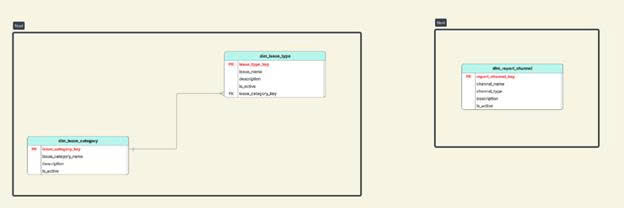
\includegraphics[width=0.9\textwidth]{Images/Picture1}
    \vspace{6mm}
    \caption{Các lược đồ Star Schema ban đầu}
\end{figure}

Cách tiếp cận theo mô hình Star Schema tách biệt này vô tình tạo nên các “ốc đảo dữ liệu” (data silos). Các bảng Dimension được tạo dựng độc lập theo từng Fact, dẫn đến tình trạng thiếu các Dimension chuẩn hóa, dùng chung. Điều này hạn chế khả năng thực hiện các phân tích đa chiều tổng hợp, đặc biệt là các phân tích chéo giữa lưu lượng giao thông và sự cố – vốn là yêu cầu quan trọng đối với bài toán ra quyết định trong thực tế.

\subsubsubsection{Thiết kế các bảng Dimension dựa trên quan sát chủ quan}
Do hạn chế về kiến thức chuyên ngành trong giai đoạn đầu, các bảng Dimension được xây dựng chủ yếu dựa trên suy luận trực quan hoặc kinh nghiệm phổ quát, thay vì trên nền tảng các quy chuẩn kỹ thuật của lĩnh vực giao thông vận tải. Điều này dẫn đến việc giản lược quá mức các thành phần mô tả, khiến các bảng chiều thiếu khả năng phản ánh đầy đủ hiện trạng vận hành giao thông.
\vspace{2mm}
Một số hạn chế điển hình bao gồm:
\\
\textbf{1. Chiều Không gian – dim\_location}
\begin{itemize}
    \item \textit{Cách tiếp cận ban đầu:} Vị trí giao thông được xem đơn thuần là một điểm địa lý (Kinh độ/Vĩ độ).
    \item \textit{Hạn chế:} Bỏ qua cấu trúc mạng lưới giao thông (Tuyến đường, Phân đoạn, Hướng lưu thông, Lý trình). Dẫn đến không thể phân tích hiện tượng ùn tắc theo chiều dài tuyến. Không thể mô tả sự khác biệt giữa hai làn đường khác nhau tại cùng tọa độ. Khó khăn trong việc đồng bộ dữ liệu từ nhiều nguồn (GPS, camera, cảm biến).

\end{itemize}

\begin{figure}[H]
    \centering
    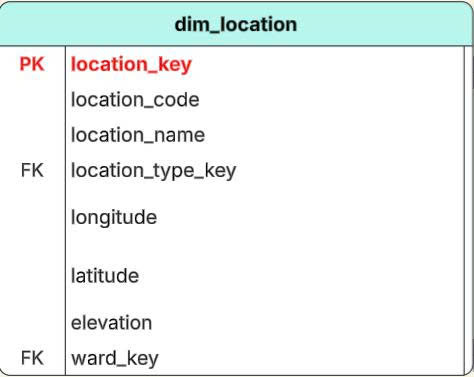
\includegraphics[width=0.5\textwidth]{Images/Picture2}
    \vspace{6mm}
    \caption{Thiết kế bảng dim\_location ban đầu}
\end{figure}

\textbf{2. Chiều Thời gian – dim\_time}
\begin{itemize}
    \item \textit{Cách tiếp cận ban đầu:} Xây dựng theo lịch dương (Giờ, Ngày, Tháng, Năm).
    \item \textit{Hạn chế:} Không phản ánh được thuộc tính đặc thù giao thông như: Giờ cao điểm/thấp điểm, Giờ cấm tải, Các ngày lễ/sự kiện, Yếu tố mùa vụ.
\end{itemize}

\begin{figure}[H]
    \centering
    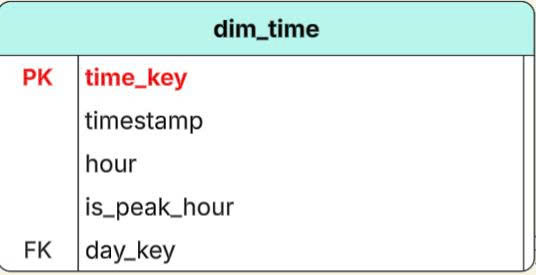
\includegraphics[width=0.5\textwidth]{Images/Picture3}
    \vspace{6mm}
    \caption{Thiết kế bảng dim\_time ban đầu}
\end{figure}

\textbf{3. Chiều Phương tiện – dim\_vehicle}
\begin{itemize}
    \item \textit{Cách tiếp cận ban đầu:} Phân loại theo tên gọi phổ biến (Xe máy, Ô tô...).
    \item \textit{Hạn chế:} Thiếu các thông số kỹ thuật (Số trục, Tải trọng, Kích thước, Hệ số PCU) cần thiết cho mô hình dự báo.
\end{itemize}

\begin{figure}[H]
    \centering
    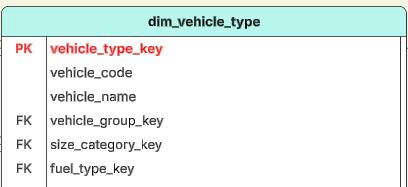
\includegraphics[width=0.5\textwidth]{Images/Picture4}
    \vspace{6mm}
    \caption{Thiết kế bảng dim\_vehicle\_type ban đầu}
\end{figure}

\subsubsubsection{Kết luận về thiết kế sơ khởi}
Thiết kế ban đầu tuy tuân thủ lý thuyết Fact-Dimension nhưng thiếu chiều sâu nghiệp vụ, tạo ra 3 hạn chế cốt lõi:
\begin{itemize}
    \item Thiếu tính liên kết giữa các quy trình nghiệp vụ (không có Dimension dùng chung).
    \item Dữ liệu mô tả nghèo nàn, thiếu phân cấp (không hỗ trợ drill-down sâu).
    \item Khả năng mở rộng thấp (khó tích hợp đa nguồn GPS/Camera).
\end{itemize}

\subsubsection{Phân tích nghiệp vụ nâng cao và xây dựng mô hình Galaxy Schema}

Sau khi nhận diện bất cập, nhóm nghiên cứu chuyển sang phân tích nghiệp vụ chuyên sâu và đề xuất mô hình \textbf{Galaxy Schema} – phù hợp khi nhiều quy trình nghiệp vụ chia sẻ chung một tập các bảng chiều chuẩn hóa.

\subsubsubsection{Phân tích ma trận nghiệp vụ}
Thông qua việc phân tích các nhóm nghiệp vụ từ BKTraffic, tài liệu liên quan, nhóm nhận thấy các luồng dữ liệu giao thông không tồn tại độc lập mà có mối quan hệ chặt chẽ với nhau. Các câu hỏi phân tích thực tế thường yêu cầu kết hợp dữ liệu từ nhiều nguồn khác nhau. Điều này làm nổi bật nhu cầu thiết kế mô hình dữ liệu tích hợp thay vì các Star Schema tách biệt.

\begin{table}[H]
\centering
\caption{Ma trận quy trình nghiệp vụ và các chiều dữ liệu}
\begin{tabular}{|l|c|c|c|c|c|c|}
\hline
\textbf{Quy trình nghiệp vụ} & \textbf{Time} & \textbf{Location} & \textbf{Vehicle} & \textbf{Weather} & \textbf{Incident} & \textbf{Source} \\ \hline
Theo dõi lưu lượng & X & X & X & X & & X \\ \hline
Giám sát sự cố & X & X & & X & X & X \\ \hline
Vận tải công cộng & X & X & X & & & \\ \hline
Dự báo thời tiết & X & X & & X & & \\ \hline
Điều phối tín hiệu & X & X & & & & X \\ \hline
\end{tabular}
\end{table}

Một số mối liên kết nghiệp vụ tiêu biểu:
\begin{itemize}
    \item Mối liên hệ giữa lưu lượng và an toàn giao thông\\
    Các nghiệp vụ như “Dự báo ùn tắc đa yếu tố” và “Đánh giá rủi ro theo khu vực” yêu cầu đồng thời thông tin về mật độ lưu thông (từ fact\_traffic\_flow) và thông tin sự cố, tai nạn (từ fact\_incident). Đây là dạng phân tích phức hợp, không thể thực hiện hiệu quả khi hai hệ thống tồn tại độc lập.
    \item Mối liên hệ giữa vận hành giao thông và yếu tố môi trường \\
    Nghiệp vụ “Dự báo giao thông theo điều kiện khí hậu” đòi hỏi tích hợp dữ liệu mưa, nhiệt độ, sương mù từ nguồn thời tiết (fact\_external\_condition) để giải thích sự biến động của tốc độ dòng xe hoặc mức độ ùn ứ.
    \item Mối liên hệ giữa sự kiện và nhu cầu giao thông\\
    Nghiệp vụ “Dự báo mật độ quanh khu vực sự kiện” yêu cầu liên kết dữ liệu về sự kiện đô thị (fact\_event) với hạ tầng giao thông, tuyến đường, phân đoạn và mật độ tại từng khu vực.

\end{itemize}

Kết quả phân tích cho thấy cần xây dựng tập Conformed Dimensions dùng chung để xóa bỏ tình trạng “ốc đảo dữ liệu”, đảm bảo các bảng fact có thể truy vấn và kết hợp dữ liệu đồng nhất.

\subsubsubsection{Tái thiết kế các Conformed Dimensions}

Để xử lý được các nghiệp vụ đa chiều và phức hợp, các bảng Dimension được tái cấu trúc với mức độ chuẩn hóa và hàm chứa ngữ nghĩa cao hơn đáng kể so với giai đoạn thiết kế ban đầu.\\

\textbf{1. Nhóm chiều Thời gian:}
Cung cấp trục thời gian đa cấp độ, liên kết toàn bộ các bảng Fact.
\begin{itemize}
    \item \texttt{dim\_date}, \texttt{dim\_date\_time}: Trục thời gian lịch và timestamp thực.
    \item \texttt{dim\_time\_of\_day}: Mô tả chi tiết 1.440 phút trong ngày, hỗ trợ bucket (5', 15').
    \item \texttt{dim\_shift}: Quản lý ca làm việc, giờ cao điểm.
    \item \texttt{dim\_holiday}, \texttt{bridge\_date\_holiday}: Quản lý ngày lễ, sự kiện đặc biệt.
\end{itemize}

\textbf{2. Nhóm chiều Không gian \& Hạ tầng:}
Hệ tọa độ chung mô tả cấu trúc phân cấp mạng lưới.
\begin{itemize}
    \item \texttt{dim\_segment}: Đơn vị cơ bản (phân đoạn đường giữa 2 node).
    \item \texttt{dim\_node}: Các nút giao, giao lộ.
    \item \texttt{dim\_route}, \texttt{bridge\_route\_segment}: Lộ trình và thứ tự segment.
    \item \texttt{dim\_way}, \texttt{dim\_road}: Cấp độ tuyến đường, trục chính.
\end{itemize}

\textbf{3. Nhóm chiều Đối tượng tham gia:}
\begin{itemize}
    \item \texttt{dim\_user}, \texttt{dim\_user\_detail}: Định danh và thuộc tính người dùng (SCD).
    \item \texttt{dim\_vehicle\_type}: Chuẩn hóa danh mục phương tiện (PCU, khí thải...).
\end{itemize}

\textbf{4. Nhóm chiều Ngữ cảnh \& Sự cố:}
\begin{itemize}
    \item \texttt{dim\_incident\_type}: Phân loại sự cố (tai nạn, ngập, công trình).
    \item \texttt{dim\_response\_unit}: Lực lượng phản ứng.
    \item \texttt{dim\_weather}: Thời tiết thực tế (mưa, gió, tầm nhìn).
\end{itemize}

\subsubsubsection{Thiết kế các bảng Fact theo nghiệp vụ}
Toàn bộ kiến trúc được tổ chức theo mô hình Galaxy Schema với 4 cụm nghiệp vụ:

\begin{itemize}
    \item \textbf{Cụm Vận hành Giao thông:}
    \begin{itemize}
        \item \texttt{fact\_traffic\_flow}: Lưu lượng tổng hợp, tốc độ trung bình, mức độ tắc nghẽn.
        \item \texttt{fact\_traffic\_flow\_by\_vehicle}: Lưu lượng chi tiết theo loại xe.
    \end{itemize}
    
    \item \textbf{Cụm Hành vi Người dùng:}
    \begin{itemize}
        \item \texttt{fact\_user\_travel\_time}: Hiệu suất di chuyển từng chuyến đi.
        \item \texttt{fact\_user\_mobility}: Thống kê hành vi tổng hợp.
    \end{itemize}
    
    \item \textbf{Cụm An toàn \& Sự cố:}
    \begin{itemize}
        \item \texttt{fact\_incident}: Ghi nhận sự cố, thời gian xử lý, mức độ nghiêm trọng.
    \end{itemize}
    
    \item \textbf{Cụm Hiệu quả Hệ thống:}
    \begin{itemize}
        \item \texttt{fact\_route\_recommendation}: Đánh giá hiệu quả gợi ý tuyến đường.
    \end{itemize}
\end{itemize}

\subsubsubsection{Tổng quan quá trình chuyển đổi}
Quá trình thiết kế là sự chuyển dịch từ: \textbf{Star Schema} (đơn giản, rời rạc) $\rightarrow$ \textbf{Snowflake Schema} (chuẩn hóa chiều không gian để phản ánh đúng topo mạng lưới) $\rightarrow$ \textbf{Galaxy Schema} (tích hợp đa luồng nghiệp vụ trên cùng hệ thống Dimension).



\subsubsection{Phân tích tính khả thi}
Phần này tập trung tìm hiểu và phân tích các nguồn data input, bao gồm 3 nguồn chính sau: TomTom, Google Maps và OpenStreetMap để xác thực độ khả thi của thiết kế tại mục 5.1.2, qua đó điều chỉnh để tính khả thi đạt 100\%.

\subsubsubsection{TomTom}

\textbf{Các loại dữ liệu và phạm vi cung cấp:} TomTom cung cấp một hệ sinh thái dữ liệu giao thông toàn diện, bao gồm cả dữ liệu thời gian thực (Real-time) với tần suất cập nhật mỗi phút và dữ liệu lịch sử phục vụ thống kê. Các nhóm dữ liệu chính bao gồm:
\begin{itemize}
    \item \textbf{Dữ liệu dòng giao thông (Traffic Flow):} Cung cấp các chỉ số về tốc độ quan sát thực tế (observed speed), thời gian di chuyển (travel time) và so sánh với tốc độ dòng chảy tự do (free-flow) cho từng phân đoạn đường (road segments).
    \item \textbf{Sự cố giao thông (Traffic Incidents):} Thông tin chi tiết về các sự kiện gây cản trở giao thông như tai nạn, công trường thi công, hoặc đường đóng. Dữ liệu bao gồm vị trí bắt đầu/kết thúc, độ dài đoạn ảnh hưởng, loại sự cố và mức độ nghiêm trọng.
    \item \textbf{Dữ liệu hiển thị và điều khiển:} Hỗ trợ các lớp bản đồ Vector Tiles cho luồng giao thông và sự cố, cùng với thông tin cập nhật giới hạn tốc độ động (Live speed restrictions) giúp tăng cường độ chính xác cho các ứng dụng dẫn đường.
\end{itemize}

\textbf{Cấu trúc và định dạng dữ liệu kỹ thuật:} Về mặt kỹ thuật, TomTom sử dụng các chuẩn dữ liệu phổ biến để đảm bảo tính tương thích cao.
\begin{itemize}
    \item Các phản hồi từ REST API (như thông tin sự cố, metadata, lỗi) được trả về dưới định dạng \textbf{JSON} tiêu chuẩn.
    \item Đối với các dữ liệu yêu cầu hiệu năng hiển thị cao như Flow/Incident Tiles, TomTom sử dụng định dạng vector nhị phân (\textbf{Binary Protobuf/PBF-like}), được tuần tự hóa bởi Google Protocol Buffers theo schema riêng.
    \item Các trường thông tin (key fields) quan trọng phục vụ cho việc mô hình hóa dữ liệu bao gồm: tọa độ không gian (\texttt{start/endLocation}), tên đường (\texttt{roadName}), tham số giao thông (\texttt{delay}, \texttt{speedObserved}, \texttt{speedFreeFlow}), độ tin cậy của dữ liệu (\texttt{confidence}) và nhãn thời gian (\texttt{timestamp}).
\end{itemize}

\textbf{Cơ chế truy cập và Chính sách sử dụng:} Để tích hợp vào hệ thống, nhà phát triển cần đăng ký API Key thông qua TomTom Developer Portal. Dữ liệu được truy xuất thông qua các RESTful API endpoints (như Traffic Incidents service) hoặc Vector Tile endpoints.
\begin{itemize}
    \item Về mặt giới hạn và chi phí, TomTom áp dụng mô hình giới hạn truy cập (Rate limits) dựa trên từng khóa API hoặc gói dịch vụ cụ thể.
    \item Mô hình chi phí dựa trên mức độ sử dụng (pay-as-you-go). Đáng chú ý, độ trễ dữ liệu (latency) được duy trì ở mức thấp, cập nhật từng phút, phù hợp cho các bài toán điều hướng thời gian thực.
\end{itemize}

\textbf{Đánh giá khả năng ứng dụng tại TP.HCM:}
\begin{itemize}
    \item \textbf{Ưu điểm:} Dữ liệu có độ tin cậy cao, cập nhật nhanh (real-time), hỗ trợ Vector Tiles giúp việc hiển thị và streaming dữ liệu lên bản đồ số mượt mà, hiệu quả. Đây là nguồn dữ liệu lý tưởng cho các ứng dụng yêu cầu độ chính xác cao như điều phối xe hoặc dẫn đường.
    \item \textbf{Nhược điểm và Thách thức:} Chi phí vận hành có thể tăng cao khi mở rộng quy mô (scale). Ngoài ra, độ phủ sóng dữ liệu (coverage) của TomTom tại TP.HCM chủ yếu tập trung tốt ở các đô thị lớn và đường trục chính; đối với hệ thống đường hẻm, đường nhánh nhỏ đặc thù của Việt Nam, lượng dữ liệu từ cảm biến/probe data có thể ít hơn.
\end{itemize}

\textbf{Kết luận:} Để tối ưu hóa hiệu quả và chi phí cho dự án, chiến lược đề xuất là chỉ sử dụng dữ liệu TomTom cho các tuyến đường trục chính, đường huyết mạch có vai trò quan trọng trong việc điều tiết giao thông toàn thành phố. Đối với các tuyến đường nhỏ hoặc hẻm không có tác động lớn đến luồng giao thông tổng thể, hệ thống sẽ cân nhắc sử dụng các nguồn dữ liệu thay thế.

\subsubsubsection{Google Maps}

\textbf{Các loại dữ liệu và phạm vi cung cấp:} Google Maps Platform cung cấp hệ sinh thái dữ liệu giao thông tập trung mạnh vào trải nghiệm dẫn đường và trực quan hóa.
\begin{itemize}
    \item \textbf{Dữ liệu giao thông thời gian thực (Real-time Traffic):} Cung cấp lớp hiển thị trực quan (\texttt{TrafficLayer}) trên bản đồ thông qua Maps JavaScript API.
    \item \textbf{Định tuyến và thời gian di chuyển (Traffic-aware Routing):} Thông qua \textbf{Directions API} và \textbf{Routes API} (\texttt{ComputeRoutes}), cung cấp ước lượng thời gian di chuyển chính xác dựa trên tình trạng giao thông thực tế.
    \item \textbf{Dữ liệu hạ tầng đường bộ:} \textbf{Roads API} hỗ trợ các tính năng như bám đường (snap-to-road), truy xuất giới hạn tốc độ (speed limits).
    \item \textbf{Lưu ý về sự cố giao thông:} Khác với TomTom, Google không cung cấp một luồng dữ liệu (feed) riêng biệt và có cấu trúc cho các sự cố (tai nạn, công trường) qua REST API.
\end{itemize}

\textbf{Cấu trúc và định dạng dữ liệu kỹ thuật:}
\begin{itemize}
    \item Các phản hồi từ REST API được trả về dưới định dạng \textbf{JSON}.
    \item Các trường thông tin quan trọng bao gồm: thời gian di chuyển trong điều kiện giao thông (\texttt{duration\_in\_traffic}), mô hình giao thông (\texttt{traffic\_model}), hình học tuyến đường (\texttt{geometry polyline}), phân đoạn hành trình (\texttt{legs/steps}) và giới hạn tốc độ (\texttt{speedLimits}).
    \item Dữ liệu có độ trễ thấp, phù hợp cao cho các tác vụ thời gian thực.
\end{itemize}

\textbf{Cơ chế truy cập và Chính sách sử dụng:} Việc truy cập dữ liệu được quản lý chặt chẽ thông qua Google Cloud Console, yêu cầu bắt buộc phải có API Key và tài khoản thanh toán (Billing account). Chi phí tính theo mô hình pay-as-you-go, khá cao cho các tính năng nâng cao như \texttt{ComputeRoutes} ở quy mô lớn.

\textbf{Đánh giá khả năng ứng dụng tại TP.HCM:}
\begin{itemize}
    \item \textbf{Ưu điểm:} Độ phủ dữ liệu (coverage) tại TP.HCM rất tốt nhờ lượng người dùng thiết bị di động khổng lồ. Khả năng tích hợp sâu với các SDK (Mobile, Web) hỗ trợ mạnh mẽ cho các bài toán định tuyến.
    \item \textbf{Nhược điểm và Thách thức:} Rào cản lớn nhất là \textbf{chi phí vận hành}. Mô hình tính phí trên mỗi yêu cầu (request-based) tạo ra gánh nặng tài chính lớn khi thu thập dữ liệu liên tục cho Data Warehouse. Ngoài ra, việc thiếu API cung cấp dữ liệu sự cố dưới dạng cấu trúc gây khó khăn cho việc thống kê tự động.
\end{itemize}

\textbf{Kết luận:} Do các hạn chế về chi phí và cấu trúc dữ liệu sự cố, Google Maps Platform được xếp độ \textbf{ưu tiên thấp nhất} trong việc làm nguồn dữ liệu đầu vào cho Kho dữ liệu. Nguồn này sẽ chỉ được cân nhắc sử dụng cho các chức năng hiển thị (Visual layer) ở phía người dùng cuối.

\subsubsubsection{OpenStreetMap}

\textbf{Các loại dữ liệu và phạm vi cung cấp:} OpenStreetMap (OSM) là cơ sở dữ liệu bản đồ nguồn mở toàn cầu. OSM cung cấp nền tảng dữ liệu địa lý tĩnh phong phú (mạng lưới đường bộ, ranh giới hành chính, POIs). Tuy nhiên, hệ thống \textbf{không cung cấp sẵn} dữ liệu lưu lượng giao thông thời gian thực hay thông tin sự cố tức thời.

\textbf{Cấu trúc và định dạng dữ liệu kỹ thuật:}
\begin{itemize}
    \item Dữ liệu OSM được tổ chức linh hoạt dựa trên mô hình thẻ (tags).
    \item Sử dụng \textbf{PBF (Protocolbuffer Binary Format)} cho lưu trữ offline và \textbf{OSM XML} hoặc \textbf{Overpass JSON} cho API.
    \item Các trường thông tin quan trọng: loại đường (\texttt{highway}), giới hạn tốc độ (\texttt{maxspeed}), chiều di chuyển (\texttt{oneway}), số làn xe (\texttt{lanes}), kết cấu mặt đường (\texttt{surface}).
\end{itemize}

\textbf{Cơ chế truy cập và Chính sách sử dụng:} OSM cung cấp cơ chế truy cập rất linh hoạt và mở (thông qua Geofabrik hoặc Overpass API). Dữ liệu hoàn toàn miễn phí dưới giấy phép \textbf{ODbL}. Chi phí thực tế chuyển dịch sang phần hạ tầng kỹ thuật (self-host) để tránh giới hạn truy cập.

\textbf{Đánh giá khả năng ứng dụng tại TP.HCM:}
\begin{itemize}
    \item \textbf{Ưu điểm:} Thế mạnh lớn nhất là độ chi tiết về hình học đường bộ, đặc biệt là hệ thống \textbf{đường hẻm, ngõ nhỏ} và lối đi bộ. Đây là nguồn dữ liệu nền tảng tuyệt vời để xây dựng đồ thị giao thông (topology graph).
    \item \textbf{Nhược điểm:} Thiếu dữ liệu traffic thời gian thực, không thể dùng độc lập để dự báo tắc nghẽn. Độ đồng nhất của dữ liệu thuộc tính tại ngoại ô có thể không cao.
\end{itemize}

\textbf{Kết luận:} OpenStreetMap là giải pháp tối ưu để giải quyết bài toán "phủ sóng" bản đồ tại các khu vực hẻm nhỏ của TP.HCM. Chiến lược đề xuất là sử dụng OSM làm \textbf{lớp bản đồ nền (Base Map)} và mạng lưới định tuyến cơ sở.

% Bảng so sánh
\begin{table}[H]
\centering
\caption{Bảng tóm tắt so sánh 3 nguồn dữ liệu}
\begin{tabular}{|p{3cm}|p{4cm}|p{4cm}|p{4cm}|}
\hline
\textbf{Tiêu chí} & \textbf{TomTom} & \textbf{Google Maps Platform} & \textbf{OpenStreetMap (OSM)} \\ \hline
Độ phủ (TP.HCM) & Rộng, commercial-grade; đường chính tốt. & Rất rộng; coverage cao ở đô thị lớn. & Geometries \& POI tốt ở khu vực cộng đồng active; mạnh về hẻm/chi tiết nhỏ. \\ \hline
Độ chính xác & Cao cho road attributes \& traffic metrics trên đường lớn. & Rất cao; enterprise-grade map + signals từ user base lớn. & Rất tốt về geometry; attribute completeness biến thiên. \\ \hline
Real-time & \textbf{Có} — real-time flow \& incident feeds (vector tiles). & \textbf{Có} — traffic-aware routing, TrafficLayer; không có incident feed công khai. & \textbf{Không} native. Cần tích hợp bên thứ ba. \\ \hline
Chi phí & Commercial — tốn phí tùy volume; pricing theo API. & Commercial — pay-as-you-go; tốn kém ở scale lớn. & \textbf{Miễn phí} (ODbL). Chi phí ở hạ tầng (hosting). \\ \hline
\end{tabular}
\end{table}

\textbf{Kiến nghị chiến lược triển khai nguồn dữ liệu thực tiễn cho TP.HCM:}
\begin{enumerate}
    \item \textbf{Lựa chọn nguồn dữ liệu cho các tác vụ thời gian thực:} Ưu tiên sử dụng \textbf{TomTom} (cho backend/data warehouse nhờ cấu trúc dữ liệu rõ ràng) hoặc \textbf{Google Maps} (cho frontend/client-side).
    \item \textbf{Chiến lược tự chủ dữ liệu và tối ưu chi phí:} Sử dụng \textbf{OpenStreetMap (OSM)} làm lớp bản đồ nền cơ sở (Base Map) để giải quyết bài toán ngân sách và đặc thù mạng lưới hẻm nhỏ.
    \item \textbf{Lộ trình kiểm thử và đánh giá tính khả thi:} Thực hiện A/B Testing và Proof of Concept (PoC) tại 1-2 quận trọng điểm để đánh giá chi phí và độ chính xác thực tế trước khi scale.
\end{enumerate}

\subsection{Kết quả}
\subsubsection{Tổng quan toàn bộ Galaxy Schema}
Mô hình Galaxy được xây dựng bằng cách sử dụng chung một tập hợp Dimensions chuẩn hóa. Tất cả các bảng Fact đều liên kết tới các Dimensions trong các chủ đề thời gian, không gian – hạ tầng, đối tượng tham gia và ngữ cảnh – sự cố, hình thành một cấu trúc phân tích đa chiều thống nhất.

\begin{figure}[H]
    \centering
    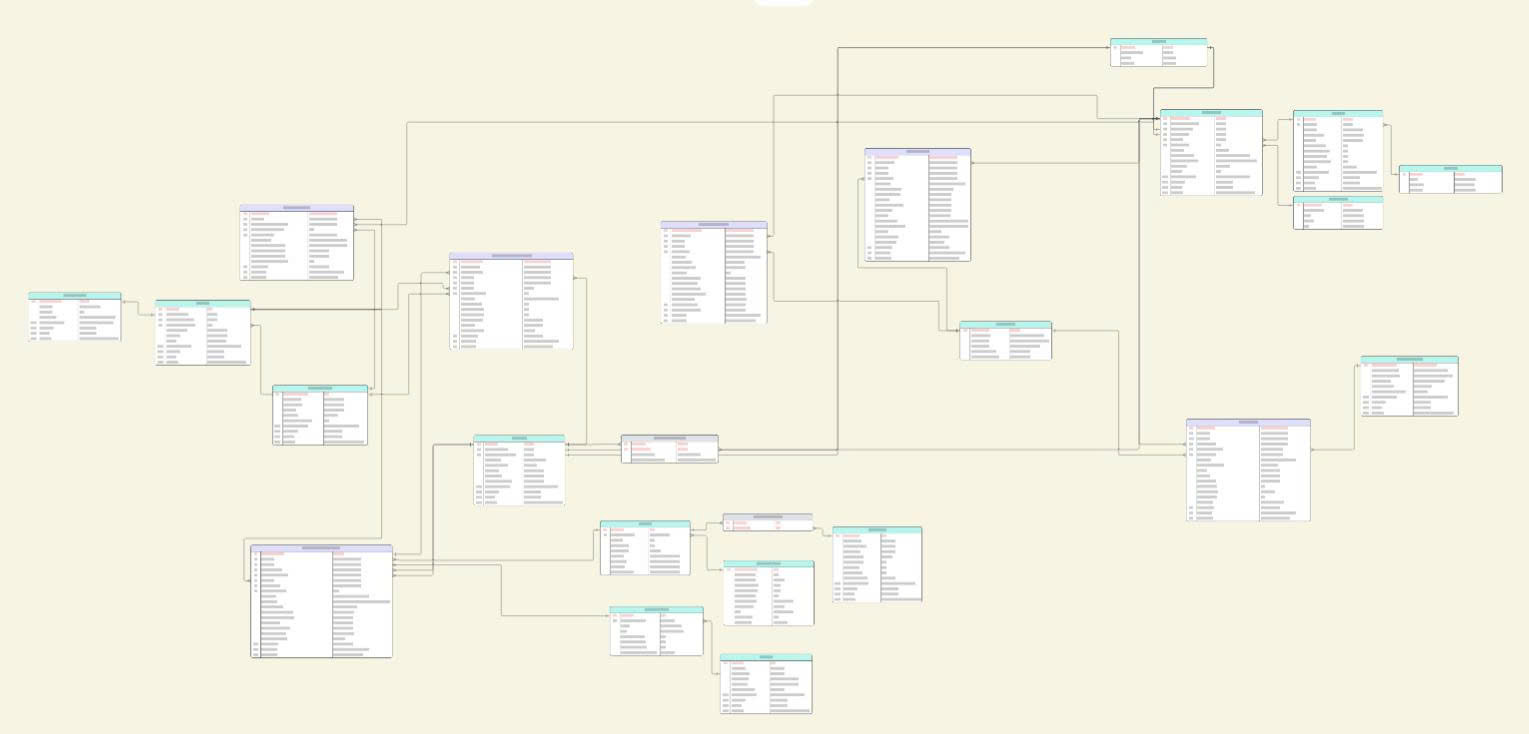
\includegraphics[width=1.0\textwidth]{Images/Picture5}
    \vspace{6mm}
    \caption{Mô hình Galaxy Schema hoàn chỉnh}
\end{figure}

\textbf{Các thành phần chính của hệ thống:}
\begin{itemize}
    \item \textbf{Hệ trục thời gian:} Bao trùm tất cả các Fact, hỗ trợ phân tích từ vi mô (phút) đến vĩ mô (năm).
    \item \textbf{Hệ tọa độ không gian – hạ tầng:} Cung cấp chuẩn tham chiếu không gian nhất quán (Segment $\rightarrow$ Node $\rightarrow$ Way $\rightarrow$ Road).
    \item \textbf{Hệ tham chiếu người dùng – phương tiện:} Phục vụ phân tích hành vi và tối ưu lộ trình.
    \item \textbf{Hệ ngữ cảnh – sự cố:} Then chốt trong phân tích an toàn và tác động môi trường.
\end{itemize}

Cách tổ chức này đảm bảo tính nhất quán dữ liệu, tăng khả năng phân tích chéo và sẵn sàng mở rộng cho các nguồn dữ liệu IoT trong tương lai.

\subsubsection{Bảng Fact}
Các ảnh bảng Fact với đầy đủ kết nối đến bảng Dim.

\begin{figure}[H]
    \centering
    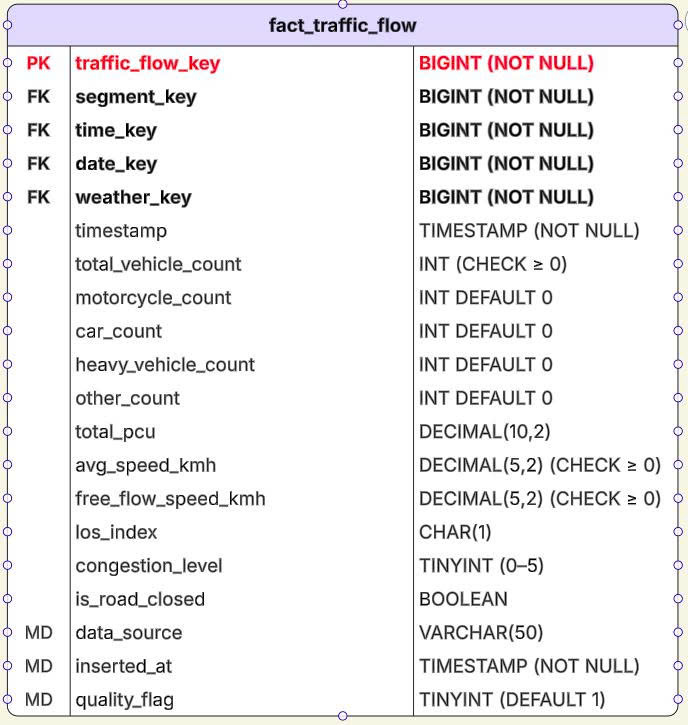
\includegraphics[width=1.0\textwidth]{Images/Picture6}
    \vspace{6mm}
    \caption{Bảng fact\_travel\_flow}
\end{figure}

\begin{figure}[H]
    \centering
   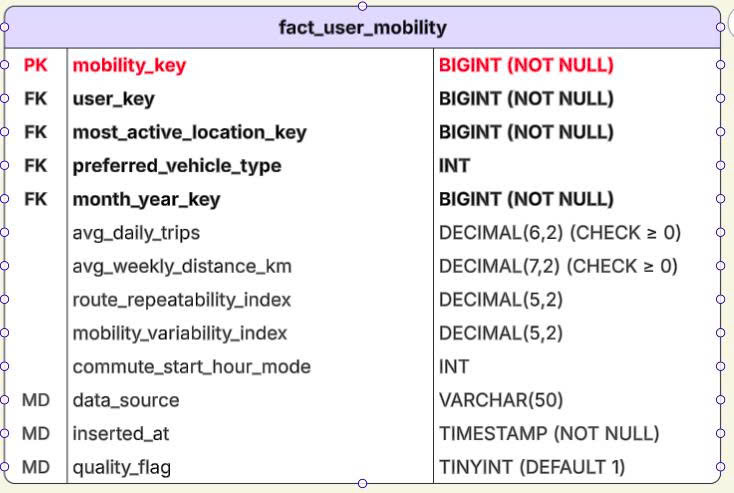
\includegraphics[width=1.0\textwidth]{Images/Picture7}
    \vspace{6mm}
    \caption{Bảng fact\_user\_mobility}
\end{figure}

\begin{figure}[H]
    \centering
    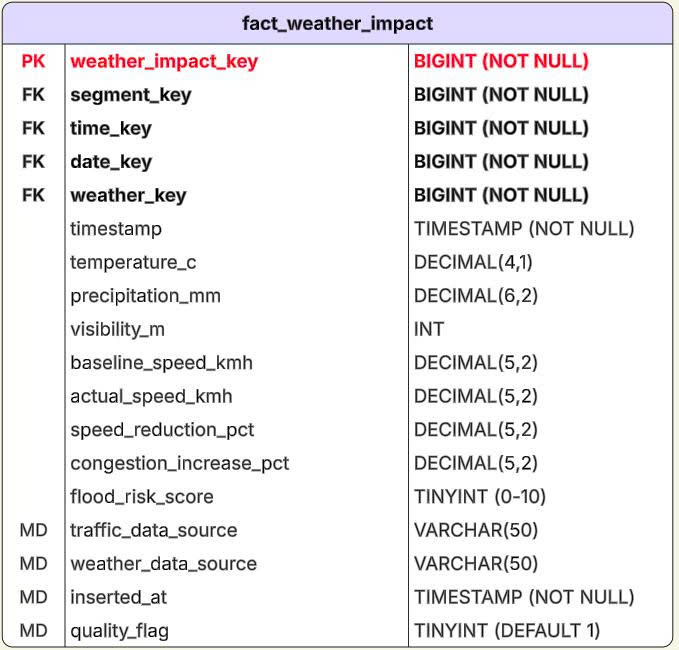
\includegraphics[width=1.0\textwidth]{Images/Picture8}
    \vspace{6mm}
    \caption{Bảng fact\_weather\_impact}
\end{figure}

\begin{figure}[H]
    \centering
   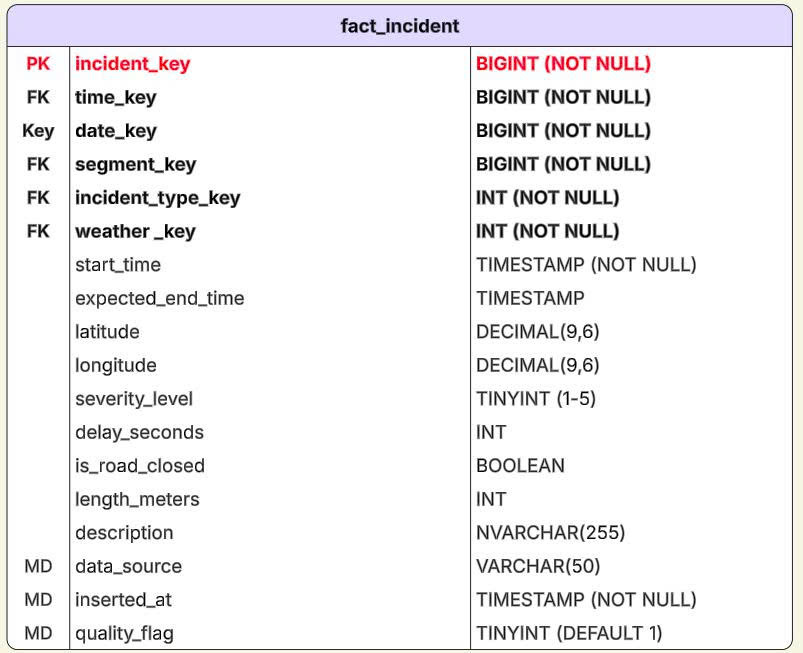
\includegraphics[width=1.0\textwidth]{Images/Picture9}
    \vspace{6mm}
    \caption{Bảng fact\_incident}
\end{figure}

\begin{figure}[H]
    \centering
    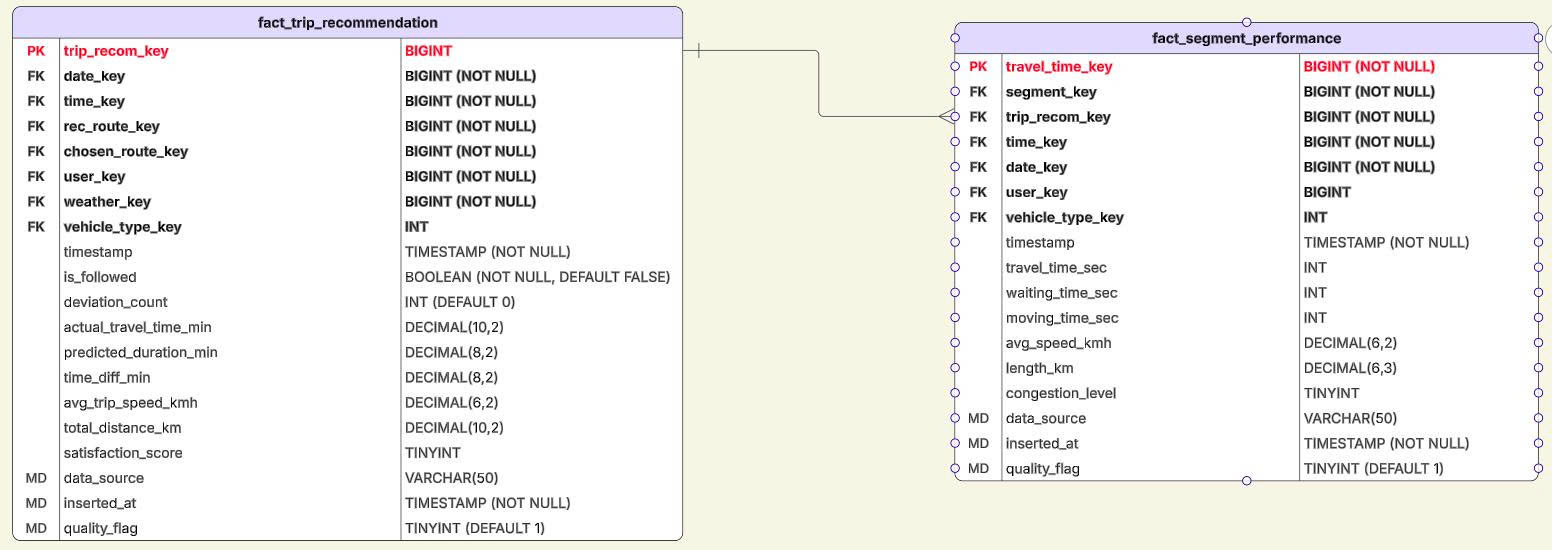
\includegraphics[width=1.0\textwidth]{Images/Picture10}
    \vspace{6mm}
    \caption{Cụm bảng fact\_trip\_recommendation và fact\_segment\_performance}
\end{figure}

\subsubsection{Bảng Dim}

\begin{figure}[H]
    \centering
    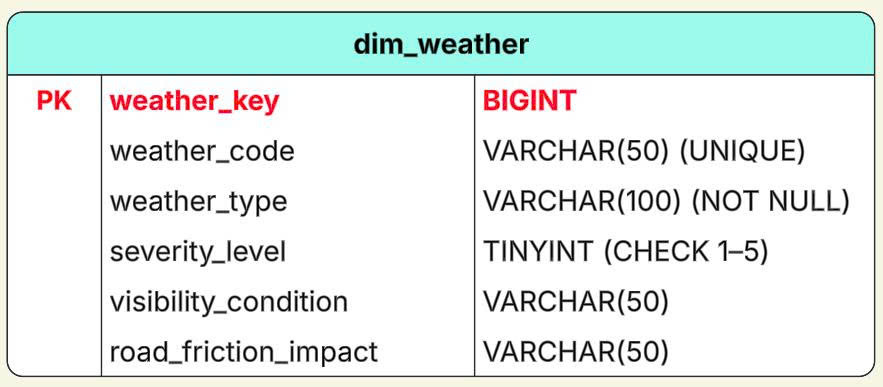
\includegraphics[width=1.0\textwidth]{Images/Picture11}
    \vspace{6mm}
    \caption{Bảng Dimension dim\_weather}
\end{figure}

\begin{figure}[H]
    \centering
    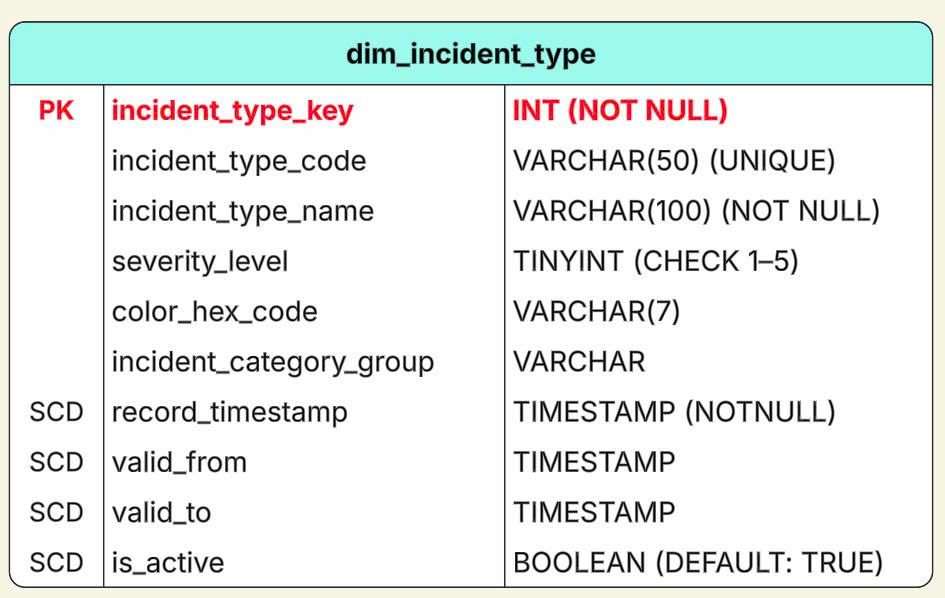
\includegraphics[width=1.0\textwidth]{Images/Picture12}
    \vspace{6mm}
    \caption{Bảng Dimension dim\_incident\_type}
\end{figure}

\begin{figure}[H]
    \centering
    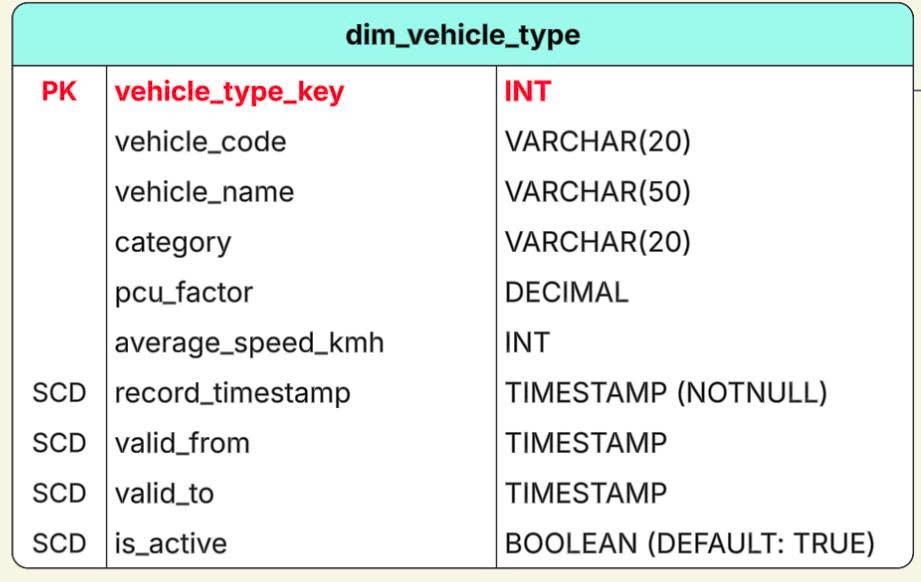
\includegraphics[width=1.0\textwidth]{Images/Picture13}
    \vspace{6mm}
    \caption{Bảng Dimension dim\_vehicle\_type}
\end{figure}

% Nhóm hình ảnh các bảng Dim liên kết (User, Time, Infrastructure)
\begin{figure}[H]
    \centering
    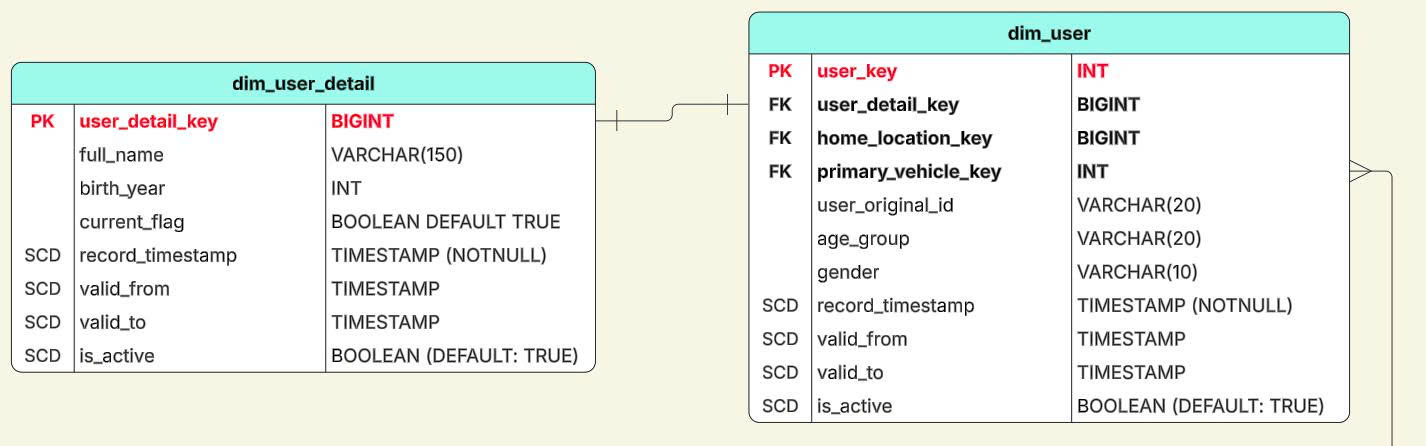
\includegraphics[width=1.0\textwidth]{Images/Picture14}
    \vspace{6mm}
    \caption{Nhóm Bảng Dimension: Người dùng}
\end{figure}

\begin{figure}[H]
    \centering
    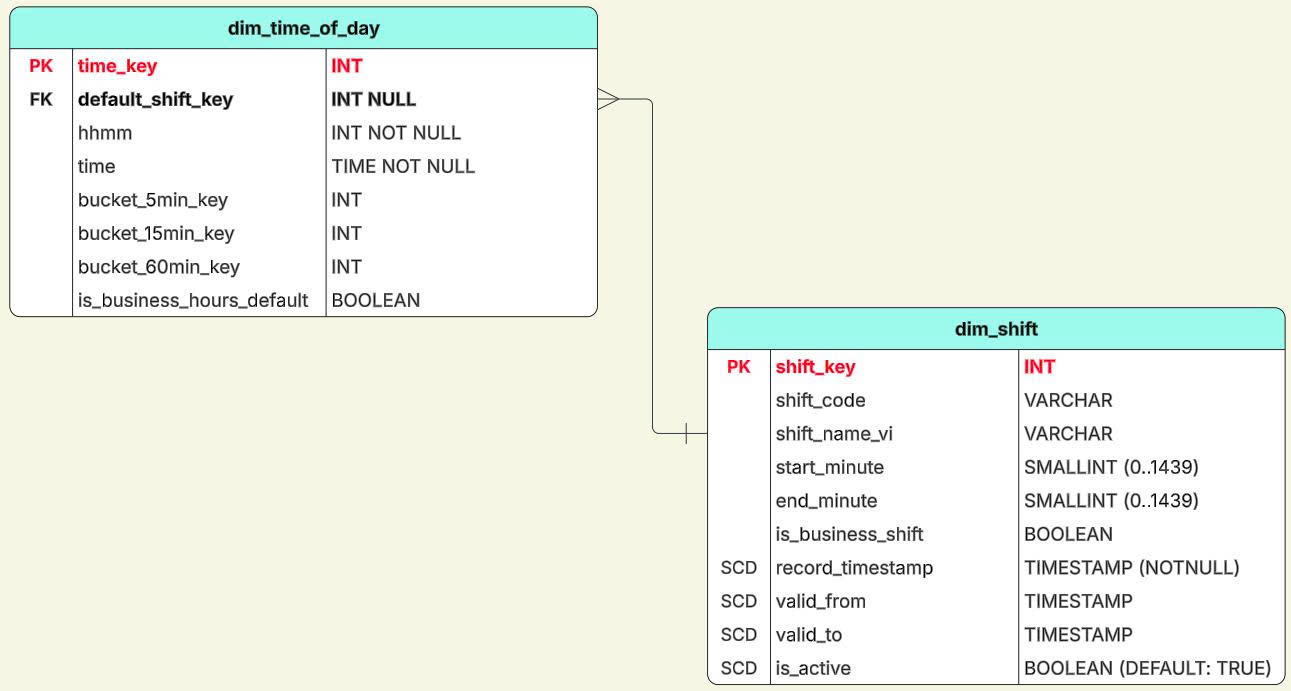
\includegraphics[width=1.0\textwidth]{Images/Picture15}
    \vspace{6mm}
    \caption{Nhóm Bảng Dimension: Thời gian (Chi tiết thời gian trong ngày)}
\end{figure}

\begin{figure}[H]
    \centering
    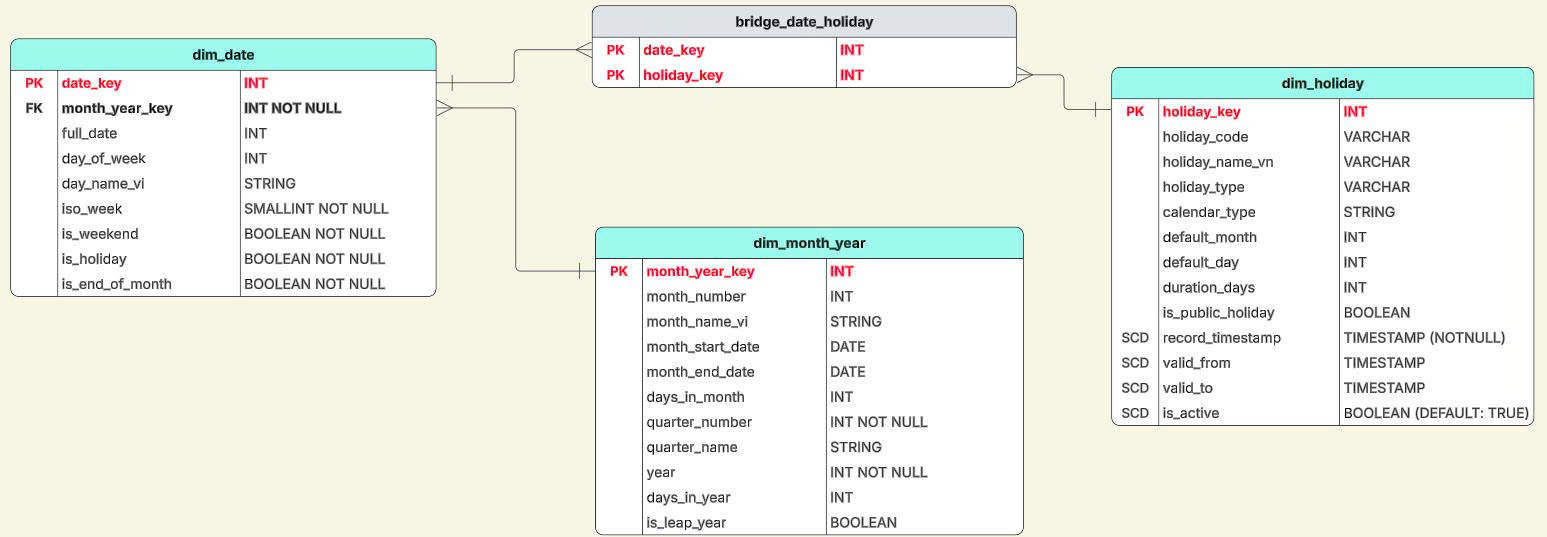
\includegraphics[width=1.0\textwidth]{Images/Picture16}
    \vspace{6mm}
    \caption{Nhóm Bảng Dimension: Thời gian (Ngày/Tháng/Năm)}
\end{figure}

\begin{figure}[H]
    \centering
    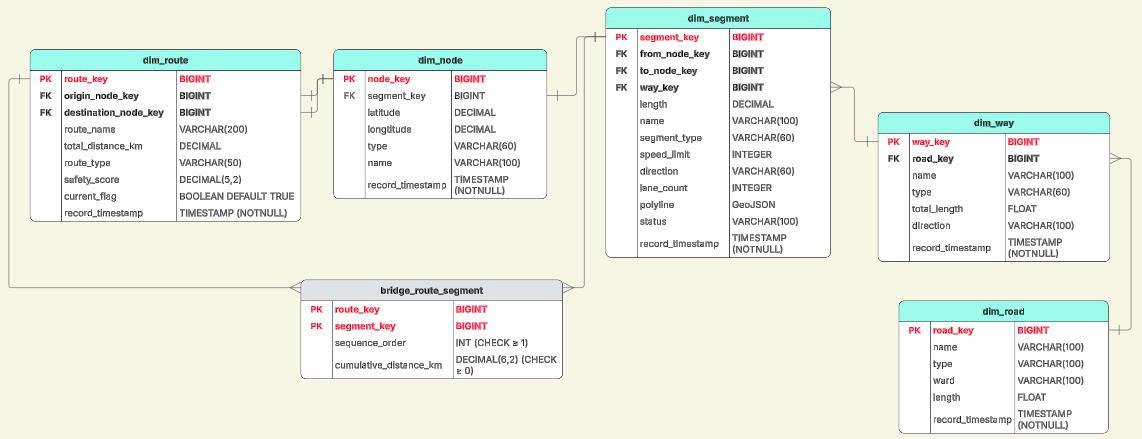
\includegraphics[width=1.0\textwidth]{Images/Picture17}
    \vspace{6mm}
    \caption{Nhóm Bảng Dimension: Hạ tầng giao thông}
\end{figure}
\subsection{Kết chương}

Chương 6 đã trình bày một cách đầy đủ tiến trình tư duy và phương pháp thiết kế kiến trúc Kho dữ liệu giao thông, thể hiện bước chuyển quan trọng từ các mô hình dữ liệu đơn giản sang một hệ kiến trúc tích hợp có tính hệ thống và đa chiều hơn.\\
Trước hết, thông qua phân tích và phản biện ở mục 5.1, nhóm nghiên cứu đã chỉ ra những hạn chế cốt lõi của việc áp dụng mô hình Lược đồ Sao rời rạc trong bối cảnh dữ liệu giao thông – nơi mà mối liên hệ giữa vận hành hạ tầng, an toàn giao thông và hành vi người dùng mang tính tương tác chặt chẽ, không thể tách biệt. Trên cơ sở đó, mô hình Galaxy Schema kết hợp với kỹ thuật chuẩn hóa chiều dạng Snowflake đã được lựa chọn và xây dựng chi tiết trong mục 5.2.\\

Thiết kế đạt được các kết quả nổi bật:
\begin{itemize}
    \item \textbf{Khắc phục phân mảnh dữ liệu:} Việc hình thành hệ thống Conformed Dimensions (như Thời gian, Segment, Phương tiện) giúp loại bỏ tình trạng rời rạc giữa các quy trình nghiệp vụ, đồng thời mở ra khả năng phân tích chéo đa lĩnh vực (cross-process analytics).
    \item \textbf{Mô hình hóa chính xác ngữ cảnh không gian:} Cấu trúc Snowflake trong nhóm chiều không gian (dim\_segment → dim\_way → dim\_road) tái hiện chính xác đặc trưng topo của mạng lưới giao thông, tạo nền tảng cho các thuật toán định tuyến, tính toán tốc độ lan truyền ùn tắc và mô phỏng sự cố.
    \item \textbf{Đáp ứng toàn diện yêu cầu nghiệp vụ:} Bốn nhóm Fact (Lưu lượng, Sự cố, Hành vi, Hiệu quả Hệ thống) bao phủ đầy đủ các nhu cầu phân tích từ giám sát thời gian thực, đánh giá vận hành, đến hỗ trợ ra quyết định chiến lược dài hạn.
\end{itemize}

Với bộ kiến trúc dữ liệu đã được định hình chắc chắn, một bài toán trọng tâm tiếp theo là xác định cách thức thu nhận dữ liệu thô từ nhiều nguồn phân tán, không đồng nhất và đưa vào hệ thống một cách nhất quán, chính xác và có khả năng mở rộng. 

\newpage
\section{Ứng dụng Schema vào thực tiễn}
\subsection{Nhóm nghiệp vụ thống kê mô tả và giám sát}
\subsubsection{A1: Giám sát tốc độ trung bình thời gian thực}

Nhóm nghiệp vụ A1 tập trung vào bài toán giám sát tốc độ trung bình của dòng giao thông theo thời gian thực, với độ trễ xử lý tối đa là 5 phút. Phân tích kỹ thuật được xây dựng dựa trên cấu trúc Kho dữ liệu (Data Warehouse) đã thiết kế, kết hợp giữa mô hình dữ liệu và các thuật toán xử lý nhằm đảm bảo độ chính xác và tính đại diện của chỉ số vận tốc được cung cấp.

\subsubsubsection{Thành phần dữ liệu trong Schema}

Để thực hiện giám sát vận tốc thực tế với độ trễ thấp, hệ thống truy vấn và tích hợp dữ liệu từ các bảng Fact và Dimension sau:\\

Bảng Fact chính: \texttt{fact\_traffic\_flow}
Bảng \texttt{fact\_traffic\_flow} đóng vai trò là nguồn dữ liệu trung tâm, lưu trữ các chỉ số giao thông được thu thập từ nhiều nguồn khác nhau (AI Camera, TomTom, v.v.). Các thuộc tính được sử dụng bao gồm:
\begin{itemize}
    \item \texttt{avg\_speed\_kmh}: Vận tốc trung bình thực tế đo được trên đoạn đường.
    \item \texttt{travel\_time\_seconds}: Thời gian di chuyển thực tế trên phân đoạn đường.
    \item \texttt{total\_pcu}: Tổng số đơn vị xe quy đổi (Passenger Car Unit), được sử dụng làm trọng số phản ánh mức độ ảnh hưởng của dòng phương tiện.
    \item \texttt{segment\_key}: Khóa định danh duy nhất cho phân đoạn đường vật lý.
    \item \texttt{time\_key}, \texttt{date\_key}: Khóa thời gian dùng để lọc dữ liệu trong cửa sổ thời gian gần thực.
    \item \texttt{quality\_flag}: Cờ đánh dấu độ tin cậy của dữ liệu, chỉ các bản ghi có giá trị bằng 1 mới được đưa vào tính toán.
\end{itemize}

Bảng Dimension hỗ trợ: \texttt{dim\_segment}
Bảng \texttt{dim\_segment} cung cấp thông tin không gian và hình học của từng phân đoạn đường:
\begin{itemize}
    \item \texttt{geometry\_linestring}: Dữ liệu hình học dạng đường (LineString), phục vụ việc hiển thị trên bản đồ.
    \item \texttt{length\_m}: Chiều dài vật lý của phân đoạn đường (đơn vị mét).
\end{itemize}

Bảng Dimension thời gian: \texttt{dim\_time\_of\_day}
Bảng \texttt{dim\_time\_of\_day} được sử dụng để gom nhóm dữ liệu theo các khoảng thời gian ngắn:
\begin{itemize}
    \item \texttt{bucket\_5min\_key}: Nhóm thời gian 5 phút, đóng vai trò là \textit{grain} (độ hạt) của báo cáo giám sát thời gian thực.
\end{itemize}

\subsubsubsection{Thuật toán xử lý dữ liệu}

Mục tiêu của thuật toán là cung cấp giá trị vận tốc định lượng chính xác cho từng phân đoạn đường, thay vì chỉ biểu diễn trạng thái giao thông bằng các mức màu định tính. Bài toán cốt lõi cần giải quyết là hội tụ dữ liệu đa nguồn trong một cửa sổ thời gian ngắn ($T = 5$ phút).\\

Vận tốc trung bình không gian

Trong kỹ thuật giao thông, vận tốc trung bình không gian (SMS) phản ánh trạng thái dòng xe chính xác hơn so với vận tốc trung bình thời gian, do SMS dựa trên tổng thời gian các phương tiện chiếm dụng đoạn đường.

Vận tốc trung bình không gian cho mỗi phân đoạn (\texttt{segment\_key}) trong một khoảng thời gian 5 phút (\texttt{bucket\_5min\_key}) được tính theo công thức:
\[
V_{SMS} = \frac{n \times L}{\sum_{i=1}^{n} t_i}
\]

Trong đó:
\begin{itemize}
    \item $L$: Chiều dài phân đoạn đường (lấy từ thuộc tính \texttt{length\_m} của bảng \texttt{dim\_segment}).
    \item $t_i$: Thời gian hành trình của phương tiện thứ $i$ (thuộc tính \texttt{travel\_time\_seconds} trong bảng \texttt{fact\_traffic\_flow}).
    \item $n$: Tổng số mẫu phương tiện được ghi nhận trong khoảng thời gian 5 phút.
\end{itemize}

Trọng số hóa theo PCU 

Do đặc thù giao thông hỗn hợp, các phương tiện có kích thước lớn như xe buýt hoặc xe tải có ảnh hưởng đáng kể hơn đến khả năng lưu thông so với xe con. Vì vậy, hệ thống áp dụng cơ chế trọng số hóa theo đơn vị xe quy đổi (PCU) nhằm tính toán vận tốc đại diện cho toàn bộ dòng xe.

Vận tốc trung bình cuối cùng cho nhóm nghiệp vụ A1 được xác định như sau:
\[
\bar{V}_{A1} = \frac{\sum_{j=1}^{m} \left( avg\_speed\_kmh_j \times total\_pcu_j \right)}{\sum_{j=1}^{m} total\_pcu_j}
\]

Trong đó:
\begin{itemize}
    \item $avg\_speed\_kmh_j$: Vận tốc đo được từ nguồn dữ liệu thứ $j$.
    \item $total\_pcu_j$: Lưu lượng xe quy đổi tương ứng của nguồn dữ liệu đó.
    \item $m$: Số lượng bản ghi dữ liệu hợp lệ được thu thập cho phân đoạn đường trong khoảng thời gian 5 phút.
\end{itemize}

Thuật toán trên cho phép hệ thống cung cấp chỉ số vận tốc có tính đại diện cao, phản ánh chính xác trạng thái thực tế của dòng giao thông trong điều kiện dữ liệu đa nguồn và thời gian xử lý gần thực.

\subsubsection{A2: Đánh giá Mức độ tắc nghẽn}

Nhóm nghiệp vụ A2 tập trung vào việc đánh giá mức độ tắc nghẽn giao thông trên từng phân đoạn đường, dựa trên hệ thống Kho dữ liệu giao thông hiện hữu. Mục tiêu của nhóm nghiệp vụ này là chuẩn hóa các chỉ số định lượng thu thập được từ dữ liệu thực tế thành các mức độ phục vụ, sau đó ánh xạ sang thang điểm trực quan từ 1 đến 5 nhằm phục vụ cho việc giám sát, phân tích và hỗ trợ ra quyết định.

\subsubsubsection{Thành phần dữ liệu trong Schema}

Để đánh giá mức độ tắc nghẽn một cách khách quan và có cơ sở khoa học, hệ thống cần kết hợp đồng thời các thuộc tính động (phản ánh trạng thái giao thông theo thời gian thực) và các thuộc tính tĩnh (phản ánh năng lực thiết kế của hạ tầng).\\

Bảng Fact chính: \texttt{fact\_traffic\_flow}
Bảng \texttt{fact\_traffic\_flow} cung cấp các chỉ số giao thông động, bao gồm:
\begin{itemize}
    \item \texttt{total\_pcu}: Tổng số đơn vị xe con quy đổi (Passenger Car Unit) đang lưu thông trên phân đoạn đường tại thời điểm quan sát.
    \item \texttt{avg\_speed\_kmh}: Tốc độ trung bình thực tế của dòng xe.
    \item \texttt{free\_flow\_speed\_kmh}: Tốc độ dòng xe trong điều kiện tự do, khi không xảy ra ùn tắc.
    \item \texttt{los\_index}: Chỉ số mức độ phục vụ (LOS từ A đến F) đã được tính toán sơ bộ từ hệ thống nguồn.
\end{itemize}

Bảng Dimension hạ tầng: \texttt{dim\_waydesign}
Bảng \texttt{dim\_waydesign} cung cấp thông tin về năng lực thiết kế của hạ tầng giao thông:
\begin{itemize}
    \item \texttt{design\_capacity}: Sức chứa thiết kế của đoạn đường, đo bằng số xe quy đổi trên giờ (PCU/giờ).
    \item \texttt{default\_speed\_limit}: Tốc độ giới hạn tối đa cho phép trên đoạn đường theo quy định.
\end{itemize}

Bảng Dimension không gian: \texttt{dim\_segment} và \texttt{dim\_location}
Hai bảng Dimension này cung cấp ngữ cảnh không gian cho việc phân tích:
\begin{itemize}
    \item \texttt{segment\_key}: Khóa định danh phân đoạn đường vật lý.
    \item \texttt{location\_key}: Khóa liên kết đến thông tin vị trí hành chính hoặc điểm giao thông đặc trưng (ví dụ: giao lộ, phường, quận).
\end{itemize}

\subsubsubsection{Thuật toán và mô hình tính toán}

Việc xác định mức độ tắc nghẽn được xây dựng dựa trên sự kết hợp của hai chỉ số cốt lõi trong kỹ thuật giao thông: tỷ lệ lưu lượng trên sức chứa (Volume-to-Capacity Ratio -- V/C) và chỉ số suy giảm vận tốc (Speed Reduction Index -- SRI). Hai chỉ số này phản ánh đồng thời áp lực hạ tầng và hành vi thực tế của dòng xe.\\

Chỉ số V/C (Volume-to-Capacity Ratio)

Chỉ số V/C thể hiện mối quan hệ giữa lưu lượng giao thông thực tế và sức chứa thiết kế của hạ tầng, được xác định theo công thức:
\[
R_{V/C} = \frac{Total\_PCU_{realtime}}{Design\_Capacity}
\]

Trong đó:
\begin{itemize}
    \item $Total\_PCU_{realtime}$ được lấy từ thuộc tính \texttt{total\_pcu} trong bảng \texttt{fact\_traffic\_flow}.
    \item $Design\_Capacity$ được lấy từ thuộc tính \texttt{design\_capacity} trong bảng \texttt{dim\_waydesign}.
\end{itemize}

Giá trị $R_{V/C}$ càng tiến gần hoặc vượt quá 1 cho thấy phân đoạn đường đang vận hành ở trạng thái quá tải so với năng lực thiết kế ban đầu.\\

Chỉ số suy giảm vận tốc (Speed Reduction Index -- SRI)

Chỉ số SRI phản ánh mức độ sụt giảm vận tốc của dòng xe so với trạng thái tự do, được tính như sau:
\[
SRI = 1 - \left( \frac{Avg\_Speed}{Free\_Flow\_Speed} \right)
\]

Trong đó:
\begin{itemize}
    \item $Avg\_Speed$ là tốc độ trung bình thực tế của dòng xe.
    \item $Free\_Flow\_Speed$ là tốc độ dòng xe trong điều kiện không bị cản trở.
\end{itemize}

Giá trị SRI nằm trong khoảng $[0,1]$. Khi SRI tiến dần về 1, dòng xe có xu hướng tiệm cận trạng thái đứng yên, phản ánh mức độ ùn tắc nghiêm trọng.

\subsubsubsection{Logic chuẩn hóa sang thang điểm 1--5}

Dựa trên tổ hợp của hai chỉ số $R_{V/C}$ và $SRI$, hệ thống thực hiện ánh xạ mức độ tắc nghẽn sang thang điểm chuẩn hóa từ 1 đến 5. Mỗi mức điểm tương ứng với một trạng thái nghiệp vụ và mức độ phục vụ (LOS) trong kỹ thuật giao thông, như trình bày trong Bảng~\ref{tab:los_mapping}.

\begin{table}[H]
\centering
\caption{Ánh xạ mức độ tắc nghẽn theo thang điểm 1--5}
\label{tab:los_mapping}
\begin{tabular}{|c|c|c|p{7cm}|}
\hline
\textbf{Mức độ} & \textbf{LOS} & \textbf{Ngưỡng $R_{V/C}$} & \textbf{Mô tả nghiệp vụ} \\ \hline
1 & A (Free Flow) & $< 0.35$ & Đường rất thông thoáng, phương tiện di chuyển gần với tốc độ giới hạn cho phép. \\ \hline
2 & B--C (Stable Flow) & $0.35 - 0.70$ & Lưu lượng ổn định, bắt đầu xuất hiện sự tương tác giữa các phương tiện. \\ \hline
3 & D (Approaching Unstable) & $0.70 - 0.85$ & Lưu lượng lớn, vận tốc giảm rõ rệt, dòng xe kém ổn định. \\ \hline
4 & E (Unstable Flow) & $0.85 - 1.00$ & Dòng xe di chuyển rất chậm, thường xuyên xảy ra hiện tượng dồn ứ. \\ \hline
5 & F (Forced Flow) & $> 1.00$ & Ùn tắc nghiêm trọng, phương tiện phải dừng chờ trong thời gian dài. \\ \hline
\end{tabular}
\end{table}

Cách tiếp cận này cho phép hệ thống chuyển đổi dữ liệu giao thông phức tạp thành các mức độ dễ diễn giải, đồng thời vẫn bảo toàn cơ sở định lượng và tính khoa học của các chỉ số kỹ thuật.


\subsubsection{A3: Phân tích thời gian di chuyển đặc trưng}

Nhóm nghiệp vụ A3 tập trung vào việc phân tích thời gian di chuyển đặc trưng của các lộ trình giao thông dựa trên dữ liệu lịch sử trong hệ thống Kho dữ liệu. Mục tiêu chính của nhóm nghiệp vụ này là xác định giá trị kỳ vọng về thời gian di chuyển cho từng lộ trình và từng khung thời gian cụ thể, từ đó làm mốc tham chiếu cho các báo cáo đánh giá hiệu suất giao thông và so sánh với điều kiện vận hành theo thời gian thực.

\subsubsubsection{Thành phần dữ liệu trong Schema}

Để thiết lập mức chuẩn về thời gian di chuyển, hệ thống cần truy vấn dữ liệu lịch sử và thực hiện phân nhóm theo các chiều thời gian và lộ trình cụ thể. Các bảng dữ liệu được sử dụng bao gồm:\\

Bảng Fact chính: \texttt{fact\_trip\_recommendation}
Bảng \texttt{fact\_trip\_recommendation} lưu trữ thông tin chi tiết của các chuyến đi đã được thực hiện trong quá khứ. Các thuộc tính được sử dụng trong phân tích bao gồm:
\begin{itemize}
    \item \texttt{chosen\_route\_key}: Khóa ngoại liên kết đến lộ trình thực tế mà người dùng đã lựa chọn và di chuyển.
    \item \texttt{actual\_travel\_time\_min}: Tổng thời gian di chuyển thực tế của chuyến đi, đơn vị phút.
    \item \texttt{time\_key}, \texttt{date\_key}: Khóa ngoại dùng để liên kết với các chiều thời gian trong Kho dữ liệu.
\end{itemize}

Bảng Dimension lộ trình: \texttt{dim\_route}
Bảng \texttt{dim\_route} cung cấp thông tin định danh và mô tả cho từng lộ trình giao thông:
\begin{itemize}
    \item \texttt{route\_key}: Định danh duy nhất cho mỗi tuyến đường.
    \item \texttt{route\_name}: Tên mô tả của lộ trình (ví dụ: ``Nhà -- Công ty'').
\end{itemize}

Bảng Dimension thời gian trong ngày: \texttt{dim\_time\_of\_day}
Bảng \texttt{dim\_time\_of\_day} được sử dụng để phân nhóm các chuyến đi theo các khung thời gian ngắn:
\begin{itemize}
    \item \texttt{bucket\_15min\_key}: Nhóm thời gian 15 phút, được xem là chuẩn phổ biến trong các nghiên cứu và hệ thống phân tích giao thông quốc tế.
\end{itemize}

Bảng Dimension ngày: \texttt{dim\_date}
Bảng \texttt{dim\_date} cung cấp ngữ cảnh lịch:
\begin{itemize}
    \item \texttt{day\_of\_week}: Thứ trong tuần (1 = Thứ Hai, $\ldots$, 7 = Chủ Nhật), cho phép phân biệt đặc tính giao thông giữa ngày thường và cuối tuần.
\end{itemize}

\subsubsubsection{Thuật toán và mô hình tính toán}

Thuật toán trong nhóm nghiệp vụ A3 tập trung vào việc trích xuất giá trị thời gian di chuyển mang tính đặc trưng, bằng cách loại bỏ các yếu tố nhiễu và các biến số cực đoan (outliers) như tai nạn giao thông, điều kiện thời tiết bất thường hoặc các sự kiện đột xuất.\\

Xác định Baseline bằng kỳ vọng toán học

Thời gian di chuyển đặc trưng $T_{Typical}$ được xác định thông qua giá trị kỳ vọng của thời gian di chuyển thực tế trong quá khứ, với điều kiện các chuyến đi có cùng đặc điểm nhận dạng về lộ trình và thời gian. Cụ thể:
\[
T_{Typical}(r, b, d) = \mathbb{E}\left[T_{actual} \mid Route = r,\; Bucket = b,\; DoW = d\right]
\]

Trong đó:
\begin{itemize}
    \item $r$: Lộ trình cụ thể, được định danh bởi \texttt{route\_key}.
    \item $b$: Khung thời gian 15 phút, tương ứng với \texttt{bucket\_15min\_key}.
    \item $d$: Thứ trong tuần, tương ứng với thuộc tính \texttt{day\_of\_week}.
\end{itemize}

Trong thực tế triển khai, giá trị kỳ vọng có thể được tính bằng trung bình cộng hoặc trung vị (median), tùy theo phân phối dữ liệu và mức độ ảnh hưởng của các giá trị ngoại lai còn sót lại.\\

Thuật toán lọc giá trị ngoại lai (Z-score Filtering)

Để đảm bảo mức chuẩn được tính toán phản ánh đúng hành vi giao thông điển hình, hệ thống áp dụng thuật toán lọc ngoại lai dựa trên chỉ số Z-score:
\[
Z = \frac{x - \mu}{\sigma}
\]

Trong đó:
\begin{itemize}
    \item $x$: Thời gian di chuyển của một chuyến đi cụ thể.
    \item $\mu$: Giá trị trung bình của thời gian di chuyển trong nhóm $(r, b, d)$.
    \item $\sigma$: Độ lệch chuẩn của thời gian di chuyển trong cùng nhóm.
\end{itemize}

Hệ thống chỉ giữ lại các bản ghi thỏa mãn điều kiện $|Z| < 2$, tương ứng với khoảng 95\% dữ liệu tập trung quanh giá trị trung bình, để phục vụ cho việc tính toán thời gian di chuyển đặc trưng.

Cách tiếp cận này cho phép xác định một giá trị baseline ổn định, có khả năng đại diện tốt cho điều kiện giao thông thông thường và đóng vai trò làm mốc so sánh tin cậy cho các phân tích hiệu suất giao thông tiếp theo.

\subsubsection{A4: Chỉ số độ tin cậy thời gian}

Nhóm nghiệp vụ A4 tập trung vào việc đánh giá độ tin cậy của thời gian di chuyển thông qua chỉ số Buffer Index (BI). Đây là một thước đo tiêu chuẩn được sử dụng rộng rãi trong lĩnh vực phân tích giao thông nhằm phản ánh mức độ biến động của thời gian hành trình. Chỉ số này hỗ trợ người sử dụng trong việc lập kế hoạch xuất phát an toàn bằng cách ước lượng khoảng thời gian dự phòng cần thiết để đảm bảo xác suất đến đúng giờ ở mức cao.

\subsubsubsection{Thành phần dữ liệu trong Schema}

Để tính toán chỉ số độ tin cậy thời gian, hệ thống cần khai thác dữ liệu hành trình lịch sử kết hợp với các khung thời gian tương ứng. Các bảng dữ liệu được sử dụng bao gồm:\\

Bảng Fact chính: \texttt{fact\_trip\_recommendation}
Bảng \texttt{fact\_trip\_recommendation} lưu trữ thông tin chi tiết về các chuyến đi đã được thực hiện trong quá khứ. Các thuộc tính chính phục vụ cho việc tính toán Buffer Index bao gồm:
\begin{itemize}
    \item \texttt{actual\_travel\_time\_min}: Thời gian di chuyển thực tế của chuyến đi (đơn vị: phút), là biến số chính phản ánh sự biến động của hành trình.
    \item \texttt{chosen\_route\_key}: Định danh tuyến đường mà người dùng đã lựa chọn để di chuyển.
    \item \texttt{time\_key}: Khóa ngoại liên kết đến chiều thời gian nhằm xác định khung giờ xuất phát.
\end{itemize}

Bảng Dimension lộ trình: \texttt{dim\_route}
Bảng \texttt{dim\_route} cung cấp thông tin định danh và mô tả cho từng tuyến đường:
\begin{itemize}
    \item \texttt{route\_key}: Khóa chính định danh duy nhất cho mỗi lộ trình.
    \item \texttt{route\_name}: Tên mô tả của lộ trình (ví dụ: ``Nhà -- Công ty'').
\end{itemize}

Bảng Dimension thời gian trong ngày: \texttt{dim\_time\_of\_day}
Bảng \texttt{dim\_time\_of\_day} được sử dụng để phân nhóm các chuyến đi theo các khung thời gian chuẩn:
\begin{itemize}
    \item \texttt{bucket\_15min\_key}: Nhóm thời gian 15 phút, được xem là hạt (grain) tiêu chuẩn để đánh giá sự biến động của thời gian di chuyển trong các khung giờ cao điểm và thấp điểm.
\end{itemize}

\subsubsubsection{Thuật toán và mô hình tính toán}

Thuật toán trọng tâm của nhóm nghiệp vụ A4 là chỉ số Buffer Index (BI), được xây dựng dựa trên sự chênh lệch giữa thời gian di chuyển trong điều kiện gần như bất lợi nhất và thời gian di chuyển trung bình. Chỉ số này phản ánh mức độ dự phòng thời gian mà người dùng cần bổ sung vào kế hoạch di chuyển để đạt được độ tin cậy mong muốn.\\

Phân vị thời gian di chuyển

Đối với mỗi cặp định danh \{\texttt{route\_key}, \texttt{bucket\_15min\_key}\}, hệ thống thu thập tập hợp các chuyến đi lịch sử với thời gian di chuyển tương ứng, ký hiệu là $T$.

Từ tập dữ liệu này, hai đại lượng thống kê quan trọng được xác định:
\begin{itemize}
    \item Thời gian di chuyển trung bình($\bar{T}$): Giá trị kỳ vọng của thời gian di chuyển, phản ánh điều kiện giao thông thông thường mà người dùng có thể gặp phải.
    \item Thời gian phân vị thứ 95 ($T_{95}$): Giá trị thời gian mà 95\% các chuyến đi trong quá khứ hoàn thành trong khoảng thời gian đó hoặc nhanh hơn. Đại lượng này đại diện cho trạng thái ``gần như tệ nhất'' mà người dùng có khả năng đối mặt trong điều kiện giao thông bất lợi.
\end{itemize}

Công thức tính chỉ số Buffer Index

Chỉ số Buffer Index được xác định theo tỷ lệ phần trăm thời gian dự phòng cần bổ sung so với thời gian trung bình, nhằm đảm bảo xác suất đến đúng giờ đạt khoảng 95\%. Công thức được biểu diễn như sau:
\[
BI(\%) = \frac{T_{95} - \bar{T}}{\bar{T}} \times 100\%
\]

Giá trị $BI$ càng lớn cho thấy mức độ biến động của thời gian di chuyển càng cao, đồng nghĩa với việc người dùng cần dành nhiều thời gian dự phòng hơn để đảm bảo độ tin cậy của hành trình. Ngược lại, giá trị $BI$ nhỏ phản ánh thời gian di chuyển ổn định và có tính dự đoán cao.

Cách tiếp cận này cho phép hệ thống lượng hóa mức độ tin cậy của thời gian di chuyển một cách trực quan, đồng thời cung cấp thông tin hữu ích cho người dùng trong việc lập kế hoạch xuất phát và đánh giá hiệu suất vận hành của mạng lưới giao thông.

\subsubsection{A5: Thống kê điểm nóng sự cố}

Nhóm nghiệp vụ A5 tập trung vào việc xác định và phân tích các điểm nóng sự cố (Incident Hotspots), hay còn gọi là các ``điểm đen'' giao thông, dựa trên dữ liệu lịch sử được lưu trữ trong hệ thống Kho dữ liệu giao thông. Mục tiêu của nhóm nghiệp vụ này là phát hiện các khu vực có tần suất và mức độ nghiêm trọng sự cố cao thông qua việc phân tích đồng thời yếu tố không gian và thời gian, từ đó hỗ trợ công tác quy hoạch, cảnh báo rủi ro và nâng cao an toàn giao thông.\\

\subsubsubsection{Thành phần dữ liệu trong Schema}

Để xác định chính xác các điểm nóng sự cố, hệ thống cần tích hợp dữ liệu từ bảng Fact sự cố và nhiều bảng Dimension hỗ trợ nhằm cung cấp đầy đủ ngữ cảnh không gian, thời gian và điều kiện ngoại cảnh.\\

Bảng Fact chính: \texttt{fact\_incident}
Bảng \texttt{fact\_incident} lưu trữ thông tin chi tiết về các sự cố giao thông đã xảy ra. Các thuộc tính chính được sử dụng trong phân tích bao gồm:
\begin{itemize}
    \item \texttt{segment\_key}: Khóa định danh phân đoạn đường nơi xảy ra sự cố.
    \item \texttt{incident\_type\_key}: Khóa ngoại liên kết đến bảng phân loại bản chất sự cố (tai nạn, xe hỏng, va chạm nhẹ, v.v.).
    \item \texttt{severity\_level}: Mức độ nghiêm trọng của sự cố, được chuẩn hóa theo thang giá trị từ 0 đến 4.
    \item \texttt{weather\_key}: Khóa ngoại dùng để liên kết với điều kiện thời tiết tại thời điểm xảy ra sự cố.
    \item \texttt{date\_key}: Khóa thời gian dùng để tích lũy và phân tích dữ liệu theo các chu kỳ báo cáo (tháng hoặc quý).
\end{itemize}

Các bảng Dimension hỗ trợ

Các bảng Dimension đóng vai trò bổ sung ngữ cảnh cho việc phân tích điểm nóng sự cố:
\begin{itemize}
    \item \texttt{dim\_incident\_type}: Cung cấp thuộc tính \texttt{incident\_category\_group}, cho phép phân nhóm các loại sự cố nghiêm trọng nhằm phục vụ phân tích chuyên sâu.
    \item \texttt{dim\_segment}: Cung cấp thông tin không gian của phân đoạn đường, bao gồm \texttt{geometry\_center} (tọa độ tâm) để xây dựng bản đồ nhiệt và \texttt{length\_m} để chuẩn hóa mật độ sự cố theo chiều dài.
    \item \texttt{dim\_weather}: Cung cấp mức độ nghiêm trọng của điều kiện thời tiết (\texttt{severity\_level}), hỗ trợ phân tích các đoạn đường nhạy cảm với yếu tố ngoại cảnh như mưa lớn, ngập lụt hoặc sương mù.
    \item \texttt{dim\_month\_year}: Cho phép lọc và nhóm dữ liệu theo các chu kỳ thời gian vĩ mô phục vụ báo cáo tổng hợp.
\end{itemize}

\subsubsubsection{Thuật toán và mô hình tính toán}

Thay vì chỉ đơn thuần đếm số lượng sự cố, nhóm nghiệp vụ A5 áp dụng phương pháp tính toán dựa trên trọng số nhằm phản ánh chính xác hơn mức độ ảnh hưởng của từng sự cố. Thuật toán cốt lõi được sử dụng là chỉ số Mật độ sự cố có trọng số (Weighted Incident Density -- WID).\\

Chỉ số cường độ sự cố (Incident Intensity Index -- III)

Mỗi sự cố $i$ được gán một trọng số $W_i$, phản ánh mức độ tác động tổng hợp của sự cố đó dựa trên mức độ nghiêm trọng của bản thân sự cố và điều kiện thời tiết tại thời điểm xảy ra. Trọng số được xác định theo công thức:
\[
W_i = (Severity\_Level_{incident} \times \alpha) + (Severity\_Level_{weather} \times \beta)
\]

Trong đó:
\begin{itemize}
    \item $Severity\_Level_{incident}$ là mức độ nghiêm trọng của sự cố giao thông.
    \item $Severity\_Level_{weather}$ là mức độ nghiêm trọng của điều kiện thời tiết tương ứng.
    \item $\alpha, \beta$ là các hệ số điều chỉnh theo quy tắc nghiệp vụ, cho phép ưu tiên các sự cố có tác động lớn hơn đến an toàn và lưu thông (ví dụ: tai nạn giao thông được gán trọng số cao hơn so với sự cố xe hỏng).
\end{itemize}

Tính toán mật độ sự cố theo không gian

Để xác định các ``điểm đen'' giao thông trên từng phân đoạn đường, hệ thống tính toán tổng trọng số sự cố tích lũy và chuẩn hóa theo chiều dài phân đoạn. Chỉ số Mật độ sự cố có trọng số cho mỗi phân đoạn được xác định như sau:
\[
WID_{segment} = \frac{\sum_{i=1}^{n} W_i}{Length\_m}
\]

Trong đó:
\begin{itemize}
    \item $n$ là tổng số sự cố xảy ra trên phân đoạn đường trong một chu kỳ phân tích (tháng hoặc quý).
    \item $Length\_m$ là chiều dài vật lý của phân đoạn đường, lấy từ bảng \texttt{dim\_segment}.
\end{itemize}

Giá trị $WID_{segment}$ càng lớn cho thấy phân đoạn đường đó có mật độ và mức độ nghiêm trọng sự cố càng cao, qua đó được xác định là một điểm nóng cần ưu tiên trong công tác giám sát, cải tạo hạ tầng hoặc triển khai các biện pháp an toàn giao thông.

\subsubsection{A6: Phân tích tác động của thời tiết đến tốc độ}

Nhóm nghiệp vụ A6 tập trung vào việc phân tích và định lượng hóa tác động của các yếu tố thời tiết đến tốc độ và năng lực thông hành của dòng xe. Các hiện tượng ngoại cảnh như mưa, sương mù hoặc bão có ảnh hưởng trực tiếp đến độ bám đường, tầm nhìn và hành vi lái xe, từ đó làm suy giảm vận tốc khai thác của hạ tầng giao thông. Mục tiêu của nhóm nghiệp vụ này là xây dựng các chỉ số định lượng phản ánh mức độ suy giảm tốc độ dưới tác động của thời tiết, đồng thời làm cơ sở cho việc dự báo và hỗ trợ ra quyết định trong quản lý giao thông.\\

\subsubsubsection{Thành phần dữ liệu trong Schema}

Để thực hiện phân tích mối tương quan giữa thời tiết và tốc độ giao thông, hệ thống kết hợp dữ liệu từ các bảng Fact đo lường vận tốc và bảng Dimension mô tả điều kiện thời tiết.\\

Bảng Fact chính: \texttt{fact\_weather\_impact}

Bảng \texttt{fact\_weather\_impact} là bảng Fact chuyên biệt được thiết kế cho nhóm nghiệp vụ A6, lưu trữ các chỉ số vận tốc trong những điều kiện thời tiết khác nhau. Các thuộc tính chính bao gồm:
\begin{itemize}
    \item \texttt{segment\_key}: Khóa ngoại định danh phân đoạn đường chịu ảnh hưởng của điều kiện thời tiết.
    \item \texttt{weather\_key}: Khóa ngoại xác định trạng thái thời tiết tại thời điểm đo (ví dụ: trời quang, mưa, sương mù).
    \item \texttt{baseline\_speed\_kmh}: Tốc độ trung bình mang tính chuẩn (baseline) của phân đoạn đường trong điều kiện thời tiết thuận lợi.
    \item \texttt{actual\_speed\_kmh}: Tốc độ trung bình thực tế được ghi nhận trong điều kiện thời tiết đang xét.
    \item \texttt{speed\_reduction\_pct}: Tỷ lệ suy giảm tốc độ đã được tính toán sẵn trong quá trình ETL.
    \item \texttt{precipitation\_mm}: Lượng mưa đo được (đơn vị: mm), phục vụ cho các phân tích định lượng theo cường độ mưa.
\end{itemize}

Bảng Fact bổ trợ: \texttt{fact\_traffic\_flow}

Bảng \texttt{fact\_traffic\_flow} cung cấp các chỉ số vận tốc nền để so sánh:
\begin{itemize}
    \item \texttt{avg\_speed\_kmh}: Tốc độ trung bình thực tế của dòng xe.
    \item \texttt{free\_flow\_speed\_kmh}: Tốc độ dòng xe trong điều kiện thông thoáng.
\end{itemize}

Bảng Dimension thời tiết: \texttt{dim\_weather}

Bảng \texttt{dim\_weather} mô tả chi tiết các đặc tính của điều kiện thời tiết:
\begin{itemize}
    \item \texttt{weather\_type}: Tên hiển thị của loại thời tiết (ví dụ: ``Mưa rào nặng hạt'').
    \item \texttt{severity\_level}: Mức độ nghiêm trọng của thời tiết, được chuẩn hóa theo thang giá trị từ 1 đến 5.
    \item \texttt{road\_friction\_impact}: Thuộc tính mô tả ảnh hưởng của thời tiết đến độ bám mặt đường (ví dụ: trơn trượt).
\end{itemize}

\subsubsubsection{Thuật toán và mô hình tính toán}

Trọng tâm của nhóm nghiệp vụ A6 là việc tính toán tỷ lệ suy giảm vận tốc (Speed Reduction Percentage -- SRP) và xây dựng mô hình tương quan giữa cường độ thời tiết và vận tốc khai thác của hạ tầng.\\

Xác định vận tốc Baseline

Thay vì sử dụng một giá trị vận tốc cố định, hệ thống xác định vận tốc baseline $V_{base}$ một cách động, dựa trên dữ liệu lịch sử của chính phân đoạn đường đó trong điều kiện thời tiết thuận lợi (trời quang), tại cùng khung thời gian trong ngày. Cụ thể:
\[
V_{base}(s, t) = \operatorname{AVG}(\texttt{avg\_speed\_kmh}) 
\;\middle|\; \text{Weather} = \text{``CLEAR''}
\]

Trong đó $s$ là phân đoạn đường (\texttt{segment\_key}) và $t$ là khung thời gian quan sát.\\

Công thức tính tỷ lệ suy giảm vận tốc

Tỷ lệ suy giảm vận tốc được tính cho từng cặp \{\texttt{segment\_key}, \texttt{weather\_type}\} theo công thức:
\[
SRP(\%) = \frac{V_{base} - V_{actual}}{V_{base}} \times 100\%
\]

Trong đó $V_{actual}$ là tốc độ trung bình thực tế được ghi nhận trong điều kiện thời tiết đang xét. Giá trị $SRP$ càng lớn phản ánh mức độ ảnh hưởng càng nghiêm trọng của thời tiết đến năng lực thông hành của đoạn đường.\\

Mô hình tương quan giữa thời tiết và vận tốc

Để phân tích sâu hơn mối quan hệ định lượng giữa cường độ mưa và tốc độ giao thông, hệ thống áp dụng mô hình hồi quy tuyến tính đơn giản:
\[
V = V_{base} - (\gamma \times P)
\]

Trong đó:
\begin{itemize}
    \item $V$ là vận tốc dự kiến của dòng xe.
    \item $P$ là lượng mưa đo được (mm).
    \item $\gamma$ là hệ số suy giảm, phản ánh mức độ nhạy cảm của vận tốc đối với lượng mưa.
\end{itemize}

Mô hình này cho phép ước lượng trước sự suy giảm tốc độ dựa trên thông tin dự báo thời tiết từ các API khí tượng, qua đó hỗ trợ hệ thống giao thông thông minh trong việc cảnh báo, điều tiết và tối ưu hóa luồng di chuyển trong điều kiện thời tiết bất lợi.

\subsubsection{A7: Đánh giá hiệu quả hệ thống gợi ý}

Nhóm nghiệp vụ A7 tập trung vào việc đánh giá mức độ hiệu quả của hệ thống gợi ý lộ trình dựa trên trí tuệ nhân tạo, thông qua việc khai thác dữ liệu trong kho dữ liệu giao thông. Mục tiêu trọng tâm của nghiệp vụ này là định lượng hóa mức độ chấp nhận, tuân thủ và mức độ tin tưởng của người dùng đối với các lộ trình được hệ thống đề xuất, từ đó làm cơ sở cho việc cải tiến thuật toán gợi ý và hỗ trợ ra quyết định ở cấp quản trị.

\subsubsubsection{Thành phần dữ liệu trong Schema}

Để đo lường hiệu quả của hệ thống gợi ý, kho dữ liệu tập trung vào các bảng Fact phản ánh hành vi sử dụng lộ trình của người dùng và kết quả phản hồi sau chuyến đi, kết hợp với bảng Dimension thời gian nhằm phục vụ phân tích xu hướng.\\

Bảng Fact chính: \texttt{fact\_trip\_recommendation}

Bảng \texttt{fact\_trip\_recommendation} lưu trữ dữ liệu ở mức hạt (grain) là mỗi chuyến đi có áp dụng gợi ý lộ trình, với các thuộc tính chính như sau:

\begin{itemize}
    \item \texttt{is\_followed}: Biến logic xác định người dùng có tuân thủ hoàn toàn lộ trình do hệ thống đề xuất hay không.
    \item \texttt{deviation\_count}: Số lần người dùng đi chệch khỏi lộ trình gợi ý trong suốt chuyến đi, phản ánh mức độ tái định tuyến.
    \item \texttt{time\_diff\_min}: Độ lệch thời gian (tính bằng phút) giữa thời gian di chuyển thực tế và thời gian dự báo bởi hệ thống AI.
    \item \texttt{satisfaction\_score}: Điểm đánh giá chủ quan của người dùng đối với lộ trình được đề xuất, theo thang đo từ 1 đến 5.
    \item \texttt{date\_key}: Khóa ngoại liên kết đến bảng Dimension thời gian, phục vụ tổng hợp và phân tích theo ngày.
\end{itemize}

Bảng Dimension thời gian: \texttt{dim\_date}

Bảng \texttt{dim\_date} cung cấp các thuộc tính thời gian hỗ trợ phân tích hiệu quả của hệ thống gợi ý theo bối cảnh sử dụng:

\begin{itemize}
    \item \texttt{date\_key}: Khóa chính dùng để liên kết với bảng Fact.
    \item \texttt{is\_weekend}, \texttt{is\_holiday}: Các biến phân loại nhằm đánh giá sự khác biệt về hiệu quả gợi ý giữa ngày thường và các ngày đặc biệt như cuối tuần hoặc ngày lễ.
\end{itemize}

\subsubsubsection{Thuật toán và mô hình tính toán}

Việc đánh giá hiệu quả của hệ thống gợi ý được thực hiện thông qua các chỉ số định lượng, phản ánh đồng thời hành vi tuân thủ của người dùng và độ chính xác kỹ thuật của mô hình dự báo.\\

Tỷ lệ Tuân thủ Lộ trình (Route Compliance Rate -- RCR)

Tỷ lệ tuân thủ lộ trình là chỉ số trực tiếp phản ánh mức độ tin tưởng của người dùng đối với các đề xuất của hệ thống. Chỉ số này được tính cho từng ngày $d$ như sau:

\[
RCR_d = \left( \frac{\sum (is\_followed = TRUE)}{Total\_Trips_d} \right) \times 100\%
\]

Trong đó $Total\_Trips_d$ là tổng số chuyến đi có áp dụng gợi ý lộ trình trong ngày $d$. Giá trị $RCR$ càng cao cho thấy mức độ chấp nhận và tin tưởng của người dùng đối với hệ thống gợi ý càng lớn.\\

Chỉ số Độ lệch Hành trình (Deviation Index -- DI)

Ngoài việc tuân thủ hoàn toàn lộ trình, hệ thống đo lường mức độ điều chỉnh của người dùng thông qua số lần tái định tuyến trung bình, được xác định như sau:

\[
DI_d = \frac{\sum_{i=1}^{n} deviation\_count_i}{Total\_Trips_d}
\]

Chỉ số $DI$ phản ánh mức độ dao động trong hành vi di chuyển. Trường hợp $RCR$ duy trì ở mức cao trong khi $DI$ lớn cho thấy lộ trình tổng thể được chấp nhận, tuy nhiên vẫn tồn tại các phân đoạn cục bộ chưa tối ưu, buộc người dùng phải điều chỉnh liên tục.\\

Độ chính xác thời gian dự kiến (ETA Accuracy)

Độ chính xác của thời gian dự kiến (Estimated Time of Arrival -- ETA) là yếu tố then chốt ảnh hưởng đến mức độ tin tưởng của người dùng. Sai số dự báo được đo lường thông qua sai số tuyệt đối trung bình (Mean Absolute Error -- MAE):

\[
MAE_{ETA} = \frac{1}{n} \sum_{i=1}^{n} \left| time\_diff\_min_i \right|
\]

Giá trị $MAE_{ETA}$ càng nhỏ cho thấy khả năng dự báo thời gian của hệ thống càng chính xác, từ đó nâng cao hiệu quả kỹ thuật và độ tin cậy của hệ thống gợi ý lộ trình.

\subsubsection{A8: Thu thập phản hồi chuyến đi }

Nhóm nghiệp vụ A8 tập trung vào việc thu thập và khai thác phản hồi sau chuyến đi của người dùng nhằm đánh giá mức độ sai lệch giữa kết quả dự báo trước chuyến đi và kết quả thực tế ghi nhận sau chuyến đi. Mục tiêu cốt lõi của nghiệp vụ này là hình thành một vòng lặp phản hồi, qua đó cung cấp dữ liệu đầu vào có giá trị cho quá trình tinh chỉnh và tái huấn luyện các mô hình học máy trong hệ thống gợi ý lộ trình.

\subsubsubsection{Thành phần dữ liệu trong Schema}

Để thực hiện đối chiếu và phân tích sai số dự báo ở cả mức độ chuyến đi và mức độ phân đoạn, hệ thống khai thác dữ liệu từ các bảng Fact chính và Fact chi tiết, kết hợp với các bảng Dimension phục vụ phân tích hành vi người dùng.\\

Bảng Fact chính: \texttt{fact\_trip\_recommendation}

Bảng \texttt{fact\_trip\_recommendation} đóng vai trò là bảng cha, lưu trữ dữ liệu tổng hợp ở mức hạt là từng chuyến đi hoàn chỉnh, với các thuộc tính quan trọng như sau:

\begin{itemize}
    \item \texttt{trip\_recom\_key}: Khóa chính định danh duy nhất cho mỗi chuyến đi có áp dụng hệ thống gợi ý.
    \item \texttt{actual\_travel\_time\_min}: Tổng thời gian di chuyển thực tế của người dùng, tính bằng phút.
    \item \texttt{predicted\_duration\_min}: Thời gian di chuyển dự kiến ban đầu do hệ thống AI tính toán trước chuyến đi.
    \item \texttt{time\_diff\_min}: Độ lệch thời gian được tính trong quá trình ETL, xác định bằng hiệu số giữa thời gian thực tế và thời gian dự báo.
    \item \texttt{satisfaction\_score}: Điểm đánh giá chủ quan của người dùng (từ 1 đến 5 sao), dùng để xác định mức độ chấp nhận sai số dự báo.
\end{itemize}

Bảng Fact chi tiết: \texttt{fact\_segment\_performance}

Bảng \texttt{fact\_segment\_performance} là bảng con, lưu trữ dữ liệu ở mức hạt chi tiết hơn, tương ứng với từng phân đoạn đường trong chuyến đi:

\begin{itemize}
    \item \texttt{travel\_time\_key}: Khóa chính đại diện cho một bản ghi phân tích hiệu suất tại mức phân đoạn.
    \item \texttt{waiting\_time\_sec}: Thời gian phương tiện đứng yên hoặc di chuyển rất chậm tại phân đoạn, phản ánh tình trạng ùn tắc cục bộ.
    \item \texttt{moving\_time\_sec}: Thời gian phương tiện thực sự di chuyển trên phân đoạn, dùng để đối chiếu với tốc độ thiết kế hoặc tốc độ dự báo.
\end{itemize}

Bảng Dimension người dùng: \texttt{dim\_user}

Bảng \texttt{dim\_user} cung cấp khóa định danh người dùng (\texttt{user\_key}), cho phép phân tích phản hồi theo từng nhóm người dùng, chẳng hạn như người dùng thường xuyên hoặc người dùng mới.

\subsubsubsection{Thuật toán và mô hình tính toán}

Các thuật toán trong nhóm nghiệp vụ A8 tập trung vào việc đo lường và phân tích sai số dự báo, từ đó xác định các điểm yếu trong mô hình định tuyến và cung cấp dữ liệu cho quá trình tối ưu hóa.\\

Sai số phần trăm tuyệt đối trung bình trên từng chuyến đi

Độ chính xác của thuật toán dự báo thời gian di chuyển được đánh giá thông qua chỉ số sai số phần trăm tuyệt đối trung bình (Mean Absolute Percentage Error -- MAPE) tại mức chuyến đi:

\[
MAPE_{trip} = \left| \frac{Actual\_Time - Predicted\_Time}{Actual\_Time} \right| \times 100\%
\]

Chỉ số này cho phép hệ thống xác định liệu sai số dự báo có nằm trong ngưỡng kỹ thuật cho phép (ví dụ nhỏ hơn 15\%) hay phản ánh sự suy giảm hiệu năng của mô hình AI trong một số bối cảnh giao thông cụ thể.\\

Phân tích nguyên nhân gốc rễ sai số (Root Cause Analysis -- RCA)

Đối với các chuyến đi có giá trị \texttt{time\_diff\_min} vượt quá ngưỡng quy định, hệ thống thực hiện truy vấn chi tiết xuống bảng \texttt{fact\_segment\_performance} nhằm xác định các phân đoạn đường đóng góp chính vào sai số dự báo. Mức độ đóng góp sai số của từng phân đoạn được xác định như sau:

\[
Error\_Contribution = 
\frac{\sum (Segment\_Actual - Segment\_Predicted)}
{Total\_Time\_Difference}
\]

Kết quả phân tích này cho phép hệ thống nhận diện các ``đoạn đường biến động'' có tần suất gây sai số cao, từ đó làm cơ sở để điều chỉnh trọng số, cập nhật tham số hoặc tái huấn luyện mô hình dự báo trong các vòng lặp học máy tiếp theo.

\subsubsection{A9: Phân bố lưu lượng theo loại xe}

Nhóm nghiệp vụ A9 tập trung vào việc phân tích cơ cấu thành phần phương tiện trong dòng giao thông nhằm hỗ trợ các quyết định điều hành và tổ chức giao thông, bao gồm phân làn chức năng, áp dụng khung giờ cấm xe và điều tiết các phương tiện có tải trọng lớn. Việc hiểu rõ tỷ trọng và mức độ chiếm dụng của từng loại xe là cơ sở quan trọng để đánh giá năng lực thông hành thực tế của hạ tầng giao thông.

\subsubsubsection{Thành phần dữ liệu trong Schema}

Để phân tích thành phần dòng xe một cách định lượng và chính xác, hệ thống khai thác dữ liệu đếm phương tiện chi tiết từ bảng Fact lưu lượng, kết hợp với các thuộc tính quy đổi và thông tin hạ tầng từ các bảng Dimension liên quan.\\

Bảng Fact chính: \texttt{fact\_traffic\_flow}

Bảng \texttt{fact\_traffic\_flow} lưu trữ các chỉ số đo lường lưu lượng phương tiện tại từng phân đoạn đường và khung thời gian, với các thuộc tính chính như sau:

\begin{itemize}
    \item \texttt{motorcycle\_count}: Số lượng xe máy được ghi nhận.
    \item \texttt{car\_count}: Số lượng xe ô tô con (dưới 9 chỗ).
    \item \texttt{heavy\_vehicle\_count}: Số lượng xe tải, xe buýt và xe container, là các phương tiện có mức độ cản trở giao thông cao.
    \item \texttt{other\_count}: Số lượng các phương tiện khác hoặc không xác định.
    \item \texttt{total\_vehicle\_count}: Tổng số lượng phương tiện thực tế ghi nhận được.
    \item \texttt{total\_pcu}: Tổng số đơn vị xe con quy đổi (Passenger Car Unit -- PCU), phản ánh tải trọng giao thông tổng hợp.
    \item \texttt{segment\_key}: Khóa định danh phân đoạn đường đang được phân tích.
\end{itemize}

Bảng Dimension phương tiện: \texttt{dim\_vehicle\_type}

Bảng \texttt{dim\_vehicle\_type} cung cấp thông tin phân loại và hệ số quy đổi cho từng loại phương tiện:

\begin{itemize}
    \item \texttt{vehicle\_name}: Tên hiển thị của loại phương tiện (ví dụ: xe máy, xe tải).
    \item \texttt{category}: Phân nhóm tổng quát như \textit{2-wheel}, \textit{4-wheel} hoặc \textit{Heavy}.
    \item \texttt{pcu\_factor}: Hệ số quy đổi đơn vị xe con, phản ánh mức độ chiếm dụng không gian và tác động đến dòng xe.
\end{itemize}

Bảng Dimension hạ tầng: \texttt{dim\_way}

Bảng \texttt{dim\_way} cung cấp các thông tin về năng lực hạ tầng nhằm đối chiếu với cơ cấu dòng xe:

\begin{itemize}
    \item \texttt{default\_lane\_count}: Số làn xe hiện hữu trên đoạn đường.
    \item \texttt{way\_type}: Loại hình đường (quốc lộ, đường đô thị nội bộ, đường vành đai), làm cơ sở áp dụng các quy định điều tiết phương tiện theo thời gian.
\end{itemize}

\subsubsubsection{Thuật toán và mô hình tính toán}

Các thuật toán trong nhóm nghiệp vụ A9 tập trung vào việc lượng hóa tỷ trọng của từng loại phương tiện trong dòng xe cũng như mức độ đóng góp của chúng vào tải trọng giao thông tổng thể.\\

Tỷ trọng thành phần phương tiện (Vehicle Mix Percentage -- VMP)

Tỷ trọng của từng loại phương tiện $i$ trên tổng lưu lượng tại một phân đoạn đường được xác định như sau:

\[
VMP_i = \frac{Count_i}{Total\_Vehicle\_Count} \times 100\%
\]

Chỉ số này cho phép nhà quản lý giao thông nhận diện loại phương tiện chiếm ưu thế trên từng tuyến đường, ví dụ như trường hợp xe máy chiếm tỷ trọng lớn trên các trục giao thông nội đô.\\

Chỉ số đóng góp tải trọng (PCU Contribution Index)

Do mức độ ảnh hưởng của các loại phương tiện đến khả năng thông hành là không đồng đều, hệ thống sử dụng chỉ số đóng góp PCU để đo lường ``không gian chiếm dụng'' thực tế của từng loại xe trong dòng giao thông:

\[
PCU\_Impact_i = 
\frac{Count_i \times PCU\_Factor_i}
{Total\_PCU}
\times 100\%
\]

Trong đó, hệ số \texttt{PCU\_Factor} được lấy từ bảng \texttt{dim\_vehicle\_type} (ví dụ: xe buýt có hệ số PCU lớn hơn xe con). Chỉ số này giúp định lượng chính xác mức độ tác động của từng nhóm phương tiện đến tình trạng ùn tắc, ngay cả khi số lượng tuyệt đối của chúng không lớn.


\subsection{Nhóm nghiệp vụ Phân tích dự báo (Predictive Analytics)}

Nhóm này không chỉ truy xuất dữ liệu quá khứ mà còn sử dụng các kỹ thuật Học máy (Machine Learning) để sinh ra tri thức mới (Insight) về trạng thái giao thông trong tương lai. Dưới đây là đặc tả kỹ thuật cho từng nghiệp vụ dự báo.

\subsubsection{Nghiệp vụ B1: Dự báo tốc độ ngắn hạn (Short-term Speed Prediction)}
\subsubsubsection{Mục đích và phạm vi}
Mục tiêu là dự đoán vận tốc trung bình (\verb|avg_speed_kmh|) cho từng đoạn đường (\verb|segment_key|) trong khoảng thời gian tương lai (T+15, T+30, T+60 phút). Kết quả dự báo là đầu vào quan trọng cho việc cảnh báo ùn tắc sớm.

\subsubsubsection{Ánh xạ dữ liệu nguồn}
Mô hình dự báo sẽ sử dụng dữ liệu lịch sử làm tập huấn luyện (Training Set). Các bảng và trường dữ liệu cụ thể bao gồm:
\begin{itemize}
    \item \textbf{Bảng Fact chính: \texttt{fact\_traffic\_flow}} (Lịch sử lưu lượng)
    \begin{itemize}
        \item \textit{Biến mục tiêu (Target Variable):} \texttt{avg\_speed\_kmh} (tại thời điểm tương lai).
        \item \textit{Biến trễ (Lag features):} Sử dụng \texttt{avg\_speed\_kmh} và \texttt{vehicle\_count} tại các thời điểm quá khứ ($t-1$, $t-2$, $t-3$) để nắm bắt xu hướng tăng/giảm của dòng xe.
    \end{itemize}
    
    \item \textbf{Bảng Dimension ngữ cảnh: \texttt{dim\_time} \& \texttt{dim\_date}}
    \begin{itemize}
        \item \textit{Tính chu kỳ:} Sử dụng \texttt{hour\_of\_day} (ví dụ: 17h chiều thường tắc đường) và \texttt{day\_of\_week} (Chủ nhật khác thứ Hai).
        \item \textit{Sự kiện đặc biệt:} Sử dụng trường \texttt{is\_holiday} trong \texttt{dim\_date} để điều chỉnh dự báo vào ngày lễ.
    \end{itemize}
    
    \item \textbf{Bảng Fact tác động: \texttt{fact\_weather\_impact}}
    \begin{itemize}
        \item \textit{Yếu tố ngoại sinh:} Sử dụng \texttt{precipitation\_mm} (lượng mưa) và \texttt{visibility\_m} (tầm nhìn) làm biến đầu vào. Mưa lớn thường làm giảm tốc độ trung bình từ 10-20\%.
    \end{itemize}
    
    \item \textbf{Bảng Dimension không gian: \texttt{dim\_segment}}
    \begin{itemize}
        \item \textit{Đặc trưng tĩnh:} Sử dụng \texttt{lane\_count} (số làn) và \texttt{road\_type} để mô hình hiểu được năng lực thông hành của đoạn đường.
    \end{itemize}
\end{itemize}

\subsubsubsection{Logic xử lý và Thuật toán}
\begin{enumerate}
    \item \textbf{Bước 1 - Data Preparation:} Thực hiện truy vấn JOIN giữa \texttt{fact\_traffic\_flow} và \texttt{fact\_weather\_impact} qua \texttt{segment\_key} và \texttt{time\_key}.
    \item \textbf{Bước 2 - Feature Engineering:} Tạo cửa sổ trượt (Sliding Window) để chuyển đổi dữ liệu chuỗi thời gian thành dạng Supervised Learning ($X$: tốc độ 30 phút trước $\rightarrow$ $Y$: tốc độ 15 phút tới).
    \item \textbf{Bước 3 - Modeling:} Áp dụng thuật toán \textbf{LSTM (Long Short-Term Memory)} hoặc \textbf{XGBoost}. Mô hình sẽ học mối tương quan phi tuyến tính: \textit{“Nếu là 17h thứ Sáu và có mưa 20mm trên đường Xô Viết Nghệ Tĩnh, tốc độ sẽ giảm xuống còn 12km/h”}.
\end{enumerate}

\subsubsection{Nghiệp vụ B2: Dự báo thời gian hành trình (ETA Prediction)}

\subsubsubsection{Mục đích và Phạm vi}
Cung cấp thời gian di chuyển dự kiến (Estimated Time of Arrival) cho một lộ trình tổng thể (Route) bao gồm nhiều đoạn đường (Segment) nối tiếp nhau.

\subsubsubsection{Ánh xạ dữ liệu nguồn}
Nghiệp vụ này là bài toán tổng hợp (Aggregation) dựa trên kết quả của B1 và cấu trúc mạng lưới đường.

\begin{itemize}
    \item \textbf{Bảng cầu nối: \texttt{bridge\_route\_segment}} (Giả định thiết kế bảng Bridge)
    \begin{itemize}
        \item \textit{Trường sử dụng:} \texttt{route\_key}, \texttt{segment\_key}, \texttt{sequence\_order} (thứ tự đoạn đường trong lộ trình).
        \item \textit{Vai trò:} Xác định lộ trình A $\rightarrow$ B bao gồm những đoạn đường nào.
    \end{itemize}
    \item \textbf{Bảng Dimension: \texttt{dim\_segment}}
    \begin{itemize}
        \item \textit{Trường sử dụng:} \texttt{length\_m} (chiều dài đoạn đường).
    \end{itemize}
    \item \textbf{Kết quả từ B1 (Dự báo tốc độ):}
    \begin{itemize}
        \item Sử dụng tốc độ dự báo \texttt{predicted\_speed\_kmh} cho từng \texttt{segment\_key}.
    \end{itemize}
\end{itemize}

\subsubsubsection{Logic xử lý và Thuật toán}
Khác với các ứng dụng bản đồ thông thường chỉ lấy tốc độ hiện tại, hệ thống này áp dụng thuật toán \textbf{Time-Dependent Routing} (Định tuyến phụ thuộc thời gian):

\begin{enumerate}
    \item \textbf{Phân rã lộ trình:} Truy vấn bảng \texttt{bridge\_route\_segment} để lấy danh sách các đoạn đường $S_1, S_2, \dots, S_n$ theo thứ tự.
    \item \textbf{Tính toán động:}
    \begin{itemize}
        \item Thời gian qua đoạn $S_1$ ($T_1$) = Chiều dài $S_1$ / Tốc độ dự báo tại thời điểm xuất phát $t_0$.
        \item Thời gian qua đoạn $S_2$ ($T_2$) = Chiều dài $S_2$ / Tốc độ dự báo tại thời điểm ($t_0 + T_1$).
        \item \textit{Lưu ý:} Tốc độ tại $S_2$ phải là tốc độ dự báo trong tương lai, không phải hiện tại.
    \end{itemize}
    \item \textbf{Tổng hợp:} 
    \[ ETA_{total} = \sum_{i=1}^{n} T_i \]
\end{enumerate}
Logic này giúp loại bỏ sai số khi người dùng bắt đầu đi lúc đường thoáng nhưng đến giữa đường thì gặp giờ cao điểm.


\subsubsection{Nghiệp vụ B3: Dự báo rủi ro sự cố (Incident Risk Prediction)}

\subsubsubsection{Mục đích và Phạm vi}
Dự đoán xác suất xảy ra tai nạn hoặc sự cố giao thông (Incident Probability) tại một thời điểm và địa điểm cụ thể, nhằm cảnh báo cho trung tâm điều hành.

\subsubsubsection{Ánh xạ dữ liệu nguồn}
Đây là bài toán Phân lớp (Classification) hoặc Hồi quy (Regression) dựa trên các mẫu hình tai nạn trong quá khứ.

\begin{itemize}
    \item \textbf{Bảng Fact sự kiện: \texttt{fact\_incident}} (Lịch sử sự cố)
    \begin{itemize}
        \item \textit{Vai trò:} Cung cấp nhãn (Label) cho mô hình học máy (Có tai nạn / Không có tai nạn).
        \item \textit{Trường sử dụng:} \texttt{incident\_type}, \texttt{severity\_level} (để phân loại mức độ rủi ro).
    \end{itemize}
    \item \textbf{Bảng Fact tác động: \texttt{fact\_weather\_impact}}
    \begin{itemize}
        \item \textit{Biến nguyên nhân:} \texttt{precipitation\_mm}, \texttt{visibility\_m}, \texttt{surface\_condition}.
        \item \textit{Logic:} Trời mưa lớn + Tầm nhìn thấp = Tăng nguy cơ va chạm.
    \end{itemize}
    \item \textbf{Bảng Fact lưu lượng: \texttt{fact\_traffic\_flow}}
    \begin{itemize}
        \item \textit{Biến nguyên nhân:} \texttt{vehicle\_count} (Mật độ). Mật độ quá cao gây va quẹt nhẹ, mật độ quá thấp nhưng tốc độ cao gây tai nạn nghiêm trọng.
    \end{itemize}
    \item \textbf{Bảng Dimension phương tiện: \texttt{dim\_vehicle\_type}} (Tham chiếu gián tiếp)
    \begin{itemize}
        \item Hệ thống phân tích tỷ lệ xe tải/container (\texttt{vehicle\_code} thuộc nhóm Heavy) trong dòng xe. Tỷ lệ xe lớn cao làm tăng chỉ số rủi ro.
    \end{itemize}
\end{itemize}

\subsubsubsection{Logic xử lý và Thuật toán}
\begin{enumerate}
    \item \textbf{Xây dựng tập dữ liệu huấn luyện:} Kết nối (Join) \texttt{fact\_incident} với dữ liệu thời tiết và lưu lượng tại cùng thời điểm xảy ra tai nạn để tạo thành các "Hồ sơ rủi ro" (Risk Profiles). Đồng thời, lấy mẫu các thời điểm bình thường (Negative samples) để cân bằng dữ liệu.
    \item \textbf{Mô hình hóa:} Sử dụng thuật toán \textbf{Random Forest} hoặc \textbf{Logistic Regression} để tính toán xác suất ($P$).
    \begin{itemize}
        \item Đầu vào: $X = \{ \text{Lượng mưa}, \text{Mật độ xe}, \text{Giờ trong ngày}, \text{Loại đường} \}$.
        \item Đầu ra: $Y = P(\text{Incident})$.
    \end{itemize}
    \item \textbf{Phân ngưỡng cảnh báo:}
    \begin{itemize}
        \item Nếu $P > 0.8$: Cảnh báo Đỏ (Nguy cơ cao).
        \item Nếu $0.5 < P \le 0.8$: Cảnh báo Vàng (Cần chú ý).
    \end{itemize}
\end{enumerate}



\subsection{Nhóm nghiệp vụ Hỗ trợ ra quyết định (Prescriptive Analytics)}

Đây là cấp độ cao nhất trong tháp phân tích dữ liệu, không chỉ dự báo tương lai mà còn trực tiếp đề xuất hành động tối ưu cho người dùng. Các nghiệp vụ này yêu cầu sự phối hợp phức tạp giữa các bảng dữ liệu lịch sử, dữ liệu dự báo và thuật toán tối ưu hóa đồ thị.

\subsubsection{Nghiệp vụ C1: Đề xuất lộ trình tối ưu đa mục tiêu (Multi-objective Routing)}

\subsubsubsection{Mục đích và Phạm vi}
Khác với các ứng dụng dẫn đường truyền thống chỉ tập trung vào "Thời gian ngắn nhất", nghiệp vụ này giải quyết bài toán đánh đổi giữa các yếu tố: \textbf{Thời gian} (Speed), \textbf{Độ tin cậy} (Reliability - tránh các đường có thời gian di chuyển biến động thất thường) và \textbf{An toàn} (Safety - tránh khu vực ngập nước hoặc hay tai nạn).

\subsubsubsection{Ánh xạ dữ liệu nguồn (Data Mapping)}
Hệ thống xây dựng hàm trọng số chi phí (Cost Function) dựa trên các bảng sau:

\begin{itemize}
    \item \textbf{Yếu tố Thời gian (Time Cost):}
    \begin{itemize}
        \item \textit{Nguồn:} Kết quả dự báo từ nghiệp vụ B1 (sử dụng \texttt{fact\_traffic\_flow}).
        \item \textit{Trường dữ liệu:} \texttt{predicted\_speed\_kmh} trên từng \texttt{segment\_key}.
    \end{itemize}
    
    \item \textbf{Yếu tố Tin cậy (Reliability Cost):}
    \begin{itemize}
        \item \textit{Nguồn:} \texttt{fact\_traffic\_flow} (Lịch sử).
        \item \textit{Logic:} Tính toán độ lệch chuẩn (Standard Deviation) của vận tốc trong cùng khung giờ quá khứ.
        \item \textit{Trường phái sinh:} Nếu độ lệch chuẩn cao $\rightarrow$ Độ tin cậy thấp (phạt điểm đoạn đường này).
    \end{itemize}
    
    \item \textbf{Yếu tố An toàn (Safety Risk Cost):}
    \begin{itemize}
        \item \textit{Nguồn 1:} \texttt{fact\_incident}. Tính tần suất tai nạn (\texttt{count}) và mức độ nghiêm trọng (\texttt{severity\_level}) trên đoạn đường.
        \item \textit{Nguồn 2:} \texttt{fact\_weather\_impact}. Nếu \texttt{precipitation\_mm} > 50mm (ngập), gán trọng số rủi ro cực đại cho các đoạn đường trũng (dựa trên thuộc tính địa hình trong \texttt{dim\_segment} nếu có, hoặc lịch sử ngập).
    \end{itemize}
\end{itemize}

\subsubsubsection{Logic xử lý và Thuật toán}
Sử dụng thuật toán tìm đường \textbf{A* (A-Star)} hoặc \textbf{Dijkstra} với hàm chi phí tổng quát:

\[ Cost_{total} = w_1 \cdot T_{dự báo} + w_2 \cdot \sigma_{biến động} + w_3 \cdot (R_{sự cố} + R_{thời tiết}) \]

Trong đó $w_1, w_2, w_3$ là các trọng số do người dùng tùy chỉnh (Ví dụ: Người dùng chọn chế độ "An toàn" thì $w_3$ sẽ tăng cao).
\begin{enumerate}
    \item \textbf{Bước 1:} Truy vấn dữ liệu từ Data Warehouse để gán trọng số cho cạnh của đồ thị giao thông.
    \item \textbf{Bước 2:} Chạy thuật toán tìm đường trên đồ thị đã gán trọng số.
    \item \textbf{Bước 3:} Trả về 3 phương án:
    \begin{itemize}
        \item \textit{Phương án 1 (Nhanh nhất):} Tối ưu hóa $w_1$.
        \item \textit{Phương án 2 (Tin cậy):} Tối ưu hóa $w_2$ (thường là các đường lớn, ít đèn đỏ, ít kẹt xe bất ngờ).
        \item \textit{Phương án 3 (An toàn):} Tối ưu hóa $w_3$ (tránh đường đang ngập hoặc hay có tai nạn).
    \end{itemize}
\end{enumerate}

\subsubsection{Nghiệp vụ C2: Cảnh báo và Tái định tuyến thời gian thực (Real-time Rerouting)}

\subsubsubsection{Mục đích và Phạm vi}
Hệ thống giám sát hành trình của người dùng và chủ động phát hiện sự cố mới phát sinh trên lộ trình dự kiến để gợi ý hướng đi vòng (Detour) ngay lập tức.

\subsubsubsection{Ánh xạ dữ liệu nguồn}
Nghiệp vụ này hoạt động theo cơ chế hướng sự kiện (Event-driven):

\begin{itemize}
    \item \textbf{Trigger (Kích hoạt):} Một bản ghi mới được INSERT vào bảng \texttt{fact\_incident}.
    \begin{itemize}
        \item \textit{Trường quan trọng:} \texttt{segment\_key} (vị trí sự cố), \texttt{incident\_type} (loại sự cố), \texttt{is\_active = TRUE}.
    \end{itemize}
    \item \textbf{Đánh giá tác động:}
    \begin{itemize}
        \item Dựa trên \texttt{dim\_segment} để xác định các đoạn đường lân cận chịu ảnh hưởng lan truyền.
        \item Dựa trên \texttt{bridge\_route\_segment} (tạm thời trong bộ nhớ) để xác định các User đang có lộ trình đi qua đoạn đường bị lỗi.
    \end{itemize}
\end{itemize}

\subsubsubsection{Logic xử lý và Thuật toán}
\begin{enumerate}
    \item \textbf{Monitoring:} Một quy trình (Daemon) liên tục lắng nghe thay đổi trên bảng \texttt{fact\_incident}.
    \item \textbf{Impact Analysis:} Khi có sự cố tại đoạn $S_{blocked}$:
    \begin{itemize}
        \item Tìm tất cả các lộ trình active $R_i$ mà $S_{blocked} \in R_i$.
    \end{itemize}
    \item \textbf{Rerouting:} Với mỗi lộ trình bị ảnh hưởng, thực hiện tìm đường lại (Re-calculation) với điều kiện:
    \[ Graph_{new} = Graph_{original} \setminus \{S_{blocked}\} \]
    (Loại bỏ cạnh bị sự cố ra khỏi đồ thị).
    \item \textbf{Notification:} Gửi thông báo đẩy: \textit{"Phát hiện tai nạn phía trước 2km. Lộ trình mới qua đường Nguyễn Thị Minh Khai nhanh hơn 10 phút."}
\end{enumerate}

\subsubsection{Nghiệp vụ C3: Gợi ý giờ xuất phát tối ưu (Optimal Departure Time)}

\subsubsubsection{Mục đích và Phạm vi}
Thay vì chỉ trả lời "Đi đường nào?", hệ thống trả lời "Đi lúc nào?". Nghiệp vụ này phân tích xu hướng tắc nghẽn trong cửa sổ thời gian (ví dụ: 2 giờ tới) để khuyến nghị người dùng dời giờ khởi hành nhằm tránh kẹt xe.

\subsubsubsection{Ánh xạ dữ liệu nguồn}
\begin{itemize}
    \item \textbf{Không gian tìm kiếm:} 1 cặp O-D (Origin - Destination) cố định.
    \item \textbf{Thời gian tìm kiếm:} $T_{start} \in [T_{now}, T_{now} + 120 \text{ phút}]$.
    \item \textbf{Dữ liệu đầu vào:}
    \begin{itemize}
        \item Kết quả dự báo B1 cho chuỗi thời gian liên tục.
        \item \texttt{dim\_time\_of\_day}: Dùng để hiển thị trục thời gian trực quan cho người dùng.
    \end{itemize}
\end{itemize}

\subsubsubsection{Logic xử lý và Thuật toán}
\begin{enumerate}
    \item \textbf{Bước 1 - Mô phỏng đa kịch bản:} Hệ thống thực hiện bài toán dự báo thời gian hành trình (B2 - ETA Prediction) lặp lại $N$ lần với các mốc thời gian xuất phát khác nhau (ví dụ: cứ mỗi 15 phút).
    \begin{itemize}
        \item $ETA_{t0}$: Xuất phát ngay bây giờ.
        \item $ETA_{t+15}$: Xuất phát sau 15 phút.
        \item ...
        \item $ETA_{t+120}$: Xuất phát sau 2 tiếng.
    \end{itemize}
    \item \textbf{Bước 2 - Tìm cực trị:} So sánh các giá trị $ETA$.
    \[ T_{optimal} = \arg \min_{t} (ETA_t + Penalty(t)) \]
    \textit{(Lưu ý: Penalty là hàm phạt nếu phải chờ đợi quá lâu, tránh việc hệ thống khuyên người dùng chờ... 3 tiếng để nhanh hơn 5 phút).}
    \item \textbf{Bước 3 - Trực quan hóa:} Vẽ biểu đồ cột so sánh thời gian di chuyển, làm nổi bật cột có thời gian thấp nhất để người dùng ra quyết định.
\end{enumerate}
\newpage
\section{Thiết kế và triển khai quy trình trích xuất, biến đổi, nạp dữ liệu (ETL)}

\subsection{Kiến trúc tổng thể hệ thống ETL}

Hệ thống ETL (Extract - Transform - Load) được thiết kế là trung tâm điều phối dữ liệu của toàn bộ dự án Traffic Data Warehouse. Kiến trúc này không chỉ đơn thuần là việc di chuyển dữ liệu, mà còn là quá trình chuẩn hóa không gian - thời gian, làm giàu dữ liệu bằng AI và tối ưu hóa cấu trúc lưu trữ để phục vụ các truy vấn phân tích phức tạp.

\subsubsection{Mục tiêu và Nguyên tắc thiết kế kiến trúc}

Hệ thống được xây dựng dựa trên các nguyên tắc thiết kế hiện đại nhằm đảm bảo tính ổn định và khả năng bảo trì lâu dài:

\begin{itemize}
    \item \textbf{Tính Module hóa (Modularity):} Toàn bộ quy trình được chia nhỏ thành các Pipeline riêng biệt: Dimension Pipeline, Mock Data Pipeline và Fact Pipeline. Cách tiếp cận này giúp cô lập lỗi và cho phép thực thi từng phần dữ liệu độc lập theo nhu cầu.
    \item \textbf{Tính nhất quán dữ liệu (Data Atomicity):} Sử dụng các cơ chế Transaction và kỹ thuật "Upsert" (Update or Insert) thông qua câu lệnh \texttt{ON CONFLICT} để đảm bảo dữ liệu không bị trùng lặp và luôn duy trì trạng thái mới nhất ngay cả khi quy trình ETL bị gián đoạn.
    \item \textbf{Tính toàn vẹn không gian (Spatial Integrity):} Mọi dữ liệu giao thông từ API đều được ánh xạ (Mapping) chính xác vào hệ hạ tầng tĩnh (Nodes, Segments) dựa trên các thuật toán hình học của PostGIS.
    \item \textbf{Khả năng mở rộng (Scalability):} Kiến trúc cho phép tích hợp thêm các nguồn dữ liệu mới như cảm biến IoT hoặc camera giao thông chỉ bằng cách bổ sung các module Service mà không cần thay đổi cấu trúc lõi của Pipeline.
\end{itemize}

\begin{figure}[htbp]
    \centering
    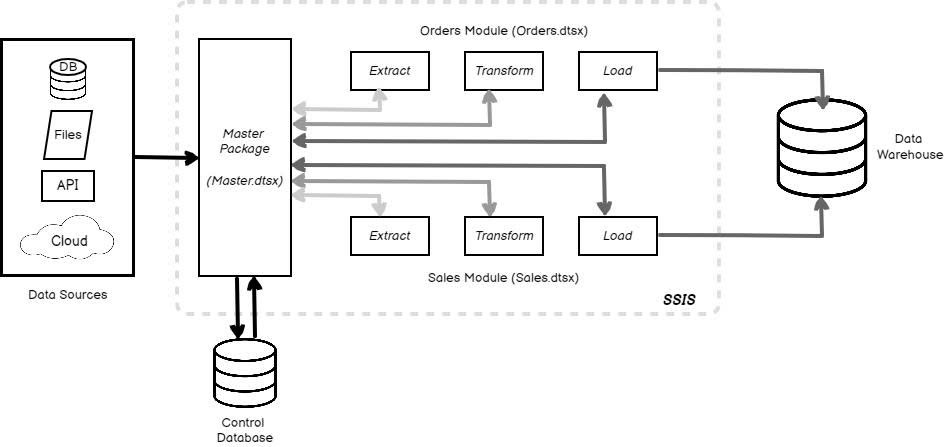
\includegraphics[width=0.8\textwidth]{Images/ETL_01}
    \vspace{6mm}
    \caption{Sơ đồ kiến trúc tổng thể hệ thống ETL}
    \label{fig:etl_01}
\end{figure}

\subsubsection{Mô hình phân lớp chức năng (Functional Layering)}

Kiến trúc ETL được tổ chức thành 4 tầng chức năng chặt chẽ:

\begin{enumerate}
    \item \textbf{Tầng thu thập (Extraction Layer):} Thực hiện kết nối và trích xuất dữ liệu đa nguồn: API thời gian thực (TomTom, OpenWeather), dữ liệu không gian (OpenStreetMap), dữ liệu nhận diện hình ảnh (YOLOv8) và dữ liệu tĩnh (CSV). Sử dụng cơ chế quản lý API Key và tham số hóa để tối ưu số lượng request (Free Tier giới hạn).
    \item \textbf{Tầng biến đổi và làm giàu (Transformation \& Enrichment Layer):} Thực hiện các phép tính toán nghiệp vụ giao thông: quy đổi lưu lượng xe sang đơn vị PCU, tính toán hướng đường (Azimuth) và xác định ranh giới hành chính bằng Spatial Join. Tích hợp mô hình học sâu YOLOv8 để chuyển đổi dữ liệu hình ảnh thô thành dữ liệu số lượng phương tiện định lượng.
    \item \textbf{Tầng lưu trữ đích (Loading Layer):} Nạp dữ liệu vào PostgreSQL. Áp dụng các kỹ thuật quản trị hiệu năng: Đánh chỉ mục không gian GIST, chỉ mục văn bản GIN và phân vùng bảng Fact theo dải thời gian (Range Partitioning).
    \item \textbf{Tầng điều phối và Giám sát (Orchestration Layer):} Sử dụng file trung tâm \texttt{main\_etl.py} kết hợp tham số dòng lệnh \texttt{--mode} để điều khiển luồng chạy. Hệ thống hóa nhật ký vận hành (Logging) để theo dõi trạng thái và thời gian thực thi của từng tác vụ.
\end{enumerate}

\subsubsection{Hạ tầng công nghệ và Thư viện lõi}

Hệ thống tận dụng sức mạnh của hệ sinh thái Python 3.12 để xử lý dữ liệu:

\begin{itemize}
    \item \textbf{Quản trị Cơ sở dữ liệu:} \texttt{psycopg2-binary} cung cấp giao thức kết nối hiệu năng cao tới PostgreSQL.
    \item \textbf{Xử lý Dữ liệu Không gian:} \texttt{OSMnx}, \texttt{GeoPandas} và \texttt{Shapely} là bộ ba công cụ dùng để trích xuất đồ thị giao thông và xử lý các đối tượng hình học phức tạp.
    \item \textbf{Xử lý AI và Thị giác máy tính:} \texttt{ultralytics} (YOLOv8) và \texttt{opencv-python-headless} được sử dụng để xây dựng bộ đếm phương tiện thông minh.
    \item \textbf{Xử lý Logic và API:} \texttt{pandas} cho các thao tác trên bảng dữ liệu lớn và \texttt{requests} để tương tác với các REST API bên ngoài.
\end{itemize}

\begin{figure}[htbp]
    \centering
    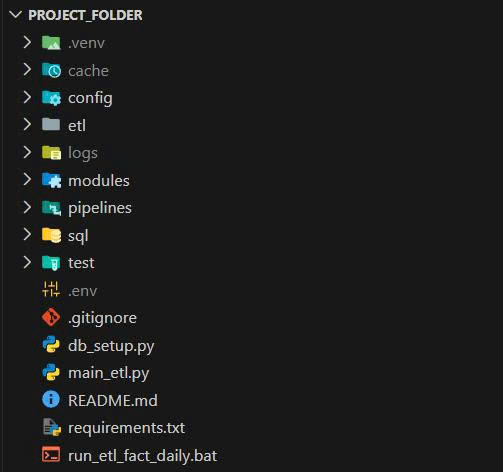
\includegraphics[width=0.6\textwidth]{Images/ETL_02}
    \vspace{6mm}
    \caption{Cấu trúc thư mục dự án hệ thống ETL}
    \label{fig:etl_02}
\end{figure}

\subsubsection{Quản lý cấu hình và Biến môi trường (Environment Configuration)}

Trong một hệ thống ETL hiện đại, việc tách biệt mã nguồn và cấu hình là nguyên tắc cốt lõi nhằm đảm bảo tính bảo mật và khả năng di động của hệ thống. Dự án triển khai cơ chế quản lý biến môi trường thông qua tệp \texttt{.env}, cho phép thay đổi tham số vận hành mà không cần can thiệp vào mã logic.

\begin{itemize}
    \item \textbf{Bảo mật thông tin nhạy cảm:} Các thông tin như thông tin đăng nhập cơ sở dữ liệu (DB\_USER, DB\_PASS) và các khóa truy cập API (TOMTOM\_API\_KEY, OWM\_API\_KEY) được lưu trữ tập trung, tránh việc lộ lọt dữ liệu khi chia sẻ mã nguồn.
    \item \textbf{Tham số hóa phạm vi dữ liệu:} Các biến như ETL\_START\_YEAR và ETL\_END\_YEAR định nghĩa khung thời gian mà hệ thống sẽ khởi tạo dữ liệu nền, giúp dễ dàng điều chỉnh quy mô kho dữ liệu theo nhu cầu phân tích.
    \item \textbf{Công nghệ thực thi:} Hệ thống sử dụng thư viện \texttt{python-dotenv} để tự động tải các biến này vào môi trường chạy của Python ngay khi khởi động.
\end{itemize}

\begin{figure}[htbp]
    \centering
    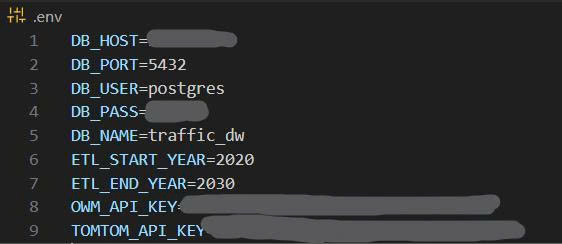
\includegraphics[width=0.7\textwidth]{Images/ETL_03}
    \vspace{6mm}
    \caption{Cấu hình các tham số trong tệp .env}
    \label{fig:etl_03}
\end{figure}

\subsubsection{Quản trị Kết nối và Tài nguyên Cơ sở dữ liệu (Connection Management)}

Để tối ưu hóa việc tương tác với PostgreSQL và đảm bảo tài nguyên hệ thống được giải phóng đúng cách, dự án xây dựng lớp \texttt{DatabaseConfig} tập trung tại \texttt{config/db\_config.py}.

\begin{itemize}
    \item \textbf{Mô hình Singleton hóa kết nối:} Thay vì khởi tạo kết nối rải rác trong từng script, hàm tĩnh \texttt{get\_connection()} cung cấp một phương thức chuẩn duy nhất để thiết lập phiên làm việc với Database.
    \item \textbf{Cơ chế xử lý lỗi kết nối:} Mã nguồn tích hợp khối lệnh \texttt{try-except} để bắt các ngoại lệ khi Database không khả dụng, giúp hệ thống đưa ra thông báo lỗi chi tiết thay vì dừng hoạt động đột ngột.
    \item \textbf{Đóng gói thông số:} Lớp này tự động đọc các biến từ \texttt{.env} (Host, Port, DB Name) để cấu hình tham số cho \texttt{psycopg2}, giúp giảm thiểu sai sót do nhập liệu thủ công trong mã nguồn.
\end{itemize}

\begin{figure}[htbp]
    \centering
    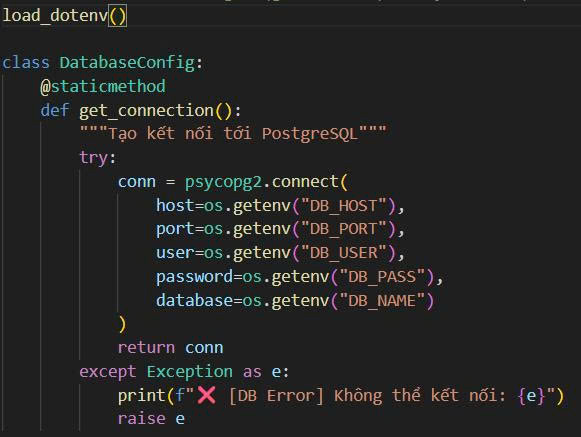
\includegraphics[width=0.8\textwidth]{Images/ETL_04}
    \vspace{6mm}
    \caption{Triển khai lớp DatabaseConfig trong Python}
    \label{fig:etl_04}
\end{figure}

\subsubsection{Cơ chế điều phối đa tầng (Hierarchical Orchestration)}

Để quản lý hàng chục script ETL một cách khoa học, hệ thống triển khai kiến trúc điều phối theo sơ đồ hình cây 3 lớp. Cơ chế này đảm bảo tính tuần tự, quản lý sự phụ thuộc và cho phép khởi chạy linh hoạt theo nhu cầu.

\begin{itemize}
    \item \textbf{Tầng 1: Bộ điều khiển trung tâm (Main Controller):} Tệp \texttt{main\_etl.py} đóng vai trò là điểm vào duy nhất (Single Entry Point) của toàn bộ hệ thống. Sử dụng \texttt{argparse} để tiếp nhận chỉ thị từ người dùng (ví dụ: \texttt{--mode all}, \texttt{--mode fact}). Tại đây, hệ thống thực hiện khởi tạo kết nối Database duy nhất và truyền phiên làm việc (Session) xuống các tầng dưới, giúp tối ưu hóa tài nguyên kết nối.
    \item \textbf{Tầng 2: Các Pipeline nhóm (Group Pipelines):} Nằm trong thư mục \texttt{pipelines/}, các script này đóng vai trò là các "nhóm trưởng" quản lý các thực thể dữ liệu có cùng tính chất:
    \begin{itemize}
        \item \texttt{run\_all\_dims.py}: Điều phối việc nạp dữ liệu nền. Nó đảm bảo các bảng không có khóa ngoại (như dim\_date) phải được chạy thành công trước khi chạy các bảng phụ thuộc (như dim\_segment).
        \item \texttt{run\_all\_facts.py}: Điều phối việc nạp dữ liệu động. Đây là pipeline quan trọng nhất trong vận hành hàng ngày, gọi đồng thời các script nạp Flow, Incident và Weather Impact.
    \end{itemize}
    \item \textbf{Tầng 3: Các Script thực thi nguyên tử (Atomic Scripts):} Đây là lớp cuối cùng nằm trong các thư mục \texttt{etl/infrastructure/}, \texttt{etl/fact/}, v.v.. Mỗi script chỉ đảm nhận một nhiệm vụ duy nhất cho một bảng cụ thể (Single Responsibility Principle), giúp việc gỡ lỗi (Debug) trở nên cực kỳ nhanh chóng.
\end{itemize}

\begin{figure}[htbp]
    \centering
    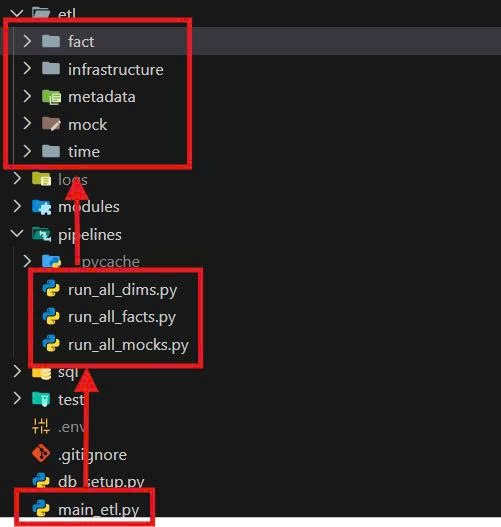
\includegraphics[width=0.6\textwidth]{Images/ETL_05}
    \vspace{6mm}
    \caption{Sơ đồ điều phối Pipeline đa tầng}
    \label{fig:etl_05}
\end{figure}

\subsection{QUY TRÌNH NẠP DỮ LIỆU DIMENSION (DIMENSION ETL PIPELINE)}

Quy trình nạp dữ liệu Dimension được thiết kế để khởi tạo "hệ quy chiếu" cho toàn bộ kho dữ liệu. Pipeline này được điều phối bởi tệp \texttt{pipelines/run\_all\_dims.py}, đảm bảo các bảng độc lập được nạp trước và các bảng có ràng buộc khóa ngoại được nạp sau theo một trình tự logic chặt chẽ.

\subsubsection{Nhóm chiều Thời gian và Lịch (Time \& Calendar Dimensions)}

Dự án triển khai một hệ thống chiều thời gian đa cấp độ, từ mức năm đến mức chi tiết từng phút trong ngày, nhằm hỗ trợ phân tích xu hướng giao thông theo các chu kỳ khác nhau.

\paragraph{Logic xử lý Lịch dương và Lịch âm (Lunar Holiday Logic)}

Việc xử lý dữ liệu thời gian trong bối cảnh giao thông tại Việt Nam đòi hỏi sự chính xác tuyệt đối về các ngày lễ, bởi đây là những thời điểm lưu lượng giao thông biến động cực đoan. Hệ thống triển khai một module chuyên biệt để giải quyết bài toán giao thoa giữa hai hệ thống lịch: Dương lịch (Solar Calendar) và Âm lịch (Lunar Calendar).

\begin{description}
    \item[A. Định nghĩa cấu trúc danh mục ngày lễ (dim\_holiday)] \hfill \\
    Dữ liệu ngày lễ không được nạp cứng mà được quản lý thông qua bảng danh mục \texttt{dim\_holiday} với các thuộc tính linh hoạt:
    \begin{itemize}
        \item \textbf{Cấu trúc lưu trữ:} Mỗi loại ngày lễ được định danh bởi một \texttt{holiday\_code} duy nhất (ví dụ: TET\_HOLIDAY, NATIONAL\_DAY).
        \item \textbf{Phân loại lịch:} Cột \texttt{calendar\_type} xác định quy tắc tính toán là 'SOLAR' hay 'LUNAR'.
        \item \textbf{Quản lý khoảng thời gian:} Thuộc tính \texttt{duration\_days} cho phép xác định một ngày lễ kéo dài bao nhiêu ngày (ví dụ: Tết Nguyên Đán kéo dài 7 ngày), giúp hệ thống tự động sinh dữ liệu cho toàn bộ kỳ nghỉ.
    \end{itemize}
\end{description}

\begin{figure}[htbp]
    \centering
    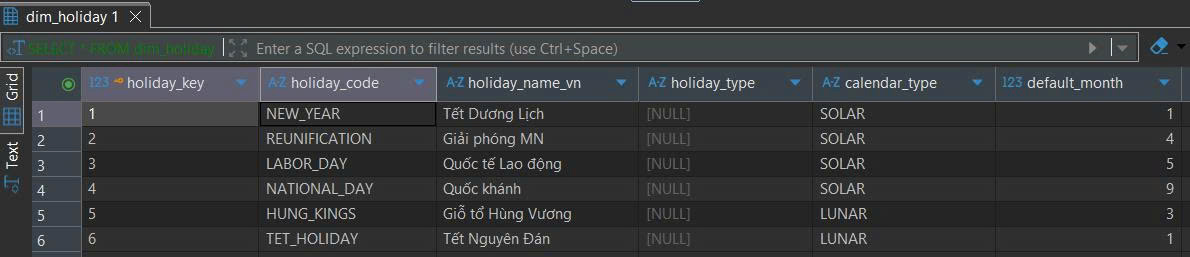
\includegraphics[width=1.0\textwidth]{Images/ETL_06}
    \caption{Dữ liệu cấu hình các ngày lễ trong bảng dim\_holiday}
    \label{fig:etl_06}
\end{figure}

\begin{description}
    \item[B. Thuật toán chuyển đổi và tính toán ngày lễ Âm lịch] \hfill \\
    Do đặc thù các ngày lễ Âm lịch không cố định theo ngày Dương lịch qua từng năm, hệ thống triển khai quy trình chuyển đổi động:
    \begin{itemize}
        \item \textbf{Tích hợp thư viện chuyên dụng:} Sử dụng thư viện \texttt{lunarcalendar} với các lớp \texttt{Converter} và \texttt{Lunar} để thực hiện phép toán chuyển đổi hệ tọa độ thời gian.
        \item \textbf{Vòng lặp tính toán:} Với mỗi năm trong cấu hình \texttt{ETL\_START\_YEAR} đến \texttt{ETL\_END\_YEAR}, hệ thống khởi tạo đối tượng \texttt{Lunar(year, month, day)} dựa trên ngày lễ định nghĩa. Sau đó, hàm \texttt{Converter.Lunar2Solar} sẽ trả về đối tượng ngày Dương lịch tương ứng.
        \item \textbf{Logic đặc thù cho Tết Nguyên Đán:} Riêng đối với mã \texttt{TET\_HOLIDAY}, hệ thống áp dụng logic lùi 1 ngày (\texttt{timedelta(days=1)}) từ mùng 1 Tết để tính toán chính xác ngày "30 Tết", đảm bảo kỳ nghỉ lễ được bắt đầu đúng thực tế văn hóa Việt Nam.
    \end{itemize}
\end{description}

\begin{figure}[htbp]
    \centering
    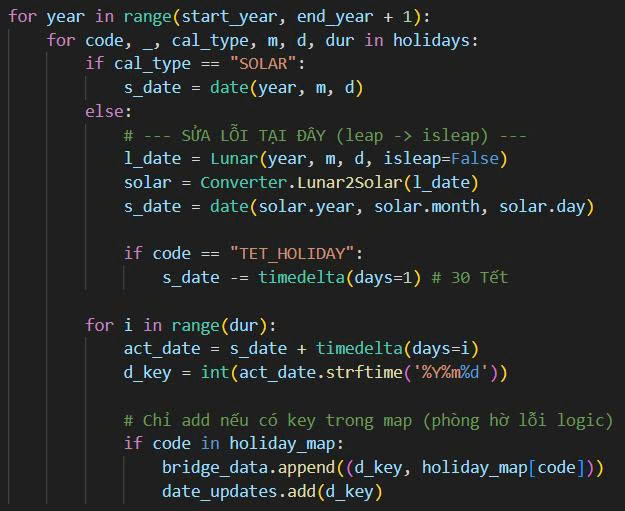
\includegraphics[width=0.7\textwidth]{Images/ETL_07}
    \vspace{6mm}
    \caption{Đoạn mã xử lý chuyển đổi lịch âm sang lịch dương cho ngày lễ}
    \label{fig:etl_07}
\end{figure}

\begin{description}
    \item[C. Cơ chế cầu nối và đồng bộ hóa (Bridge Mechanism)] \hfill \\
    Để giải quyết mối quan hệ nhiều-nhiều (N-N) giữa Ngày và Lễ (một ngày có thể có nhiều lễ, hoặc một lễ kéo dài nhiều ngày), hệ thống sử dụng bảng cầu nối \texttt{bridge\_date\_holiday}:
    \begin{itemize}
        \item \textbf{Ánh xạ khóa ngoại:} Mỗi cặp \texttt{date\_key} (từ \texttt{dim\_date}) và \texttt{holiday\_key} (từ \texttt{dim\_holiday}) được ghi nhận để xác định chính xác sự hiện diện của ngày lễ.
        \item \textbf{Tối ưu hóa hiệu suất truy vấn (De-normalization):} Sau khi nạp dữ liệu vào bảng cầu nối, hệ thống thực hiện một lệnh \texttt{UPDATE} tập hợp lên bảng \texttt{dim\_date}. Toàn bộ các \texttt{date\_key} xuất hiện trong bảng cầu nối sẽ được bật cờ \texttt{is\_holiday = TRUE}.
        \item \textbf{Lợi ích:} Kỹ thuật này giúp các câu lệnh truy vấn lưu lượng giao thông trong ngày lễ sau này chỉ cần lọc theo cờ \texttt{is\_holiday} mà không cần thực hiện phép \texttt{JOIN} phức tạp, giúp tăng tốc độ phản hồi của hệ thống báo cáo.
    \end{itemize}
\end{description}

\begin{figure}[htbp]
    \centering
    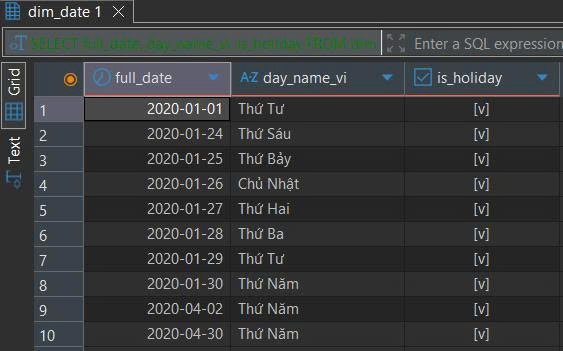
\includegraphics[width=0.7\textwidth]{Images/ETL_08}
    \vspace{6mm}
    \caption{Kết quả cập nhật cờ is\_holiday trong bảng dim\_date}
    \label{fig:etl_08}
\end{figure}

\paragraph{Phân tách và ánh xạ Ca làm việc (Work Shifts)}

Trong phân tích dữ liệu giao thông, việc chỉ sử dụng các mốc giờ thô là không đủ để phản ánh đặc tính vận hành của đô thị. Hệ thống triển khai giải pháp phân tách thời gian dựa trên các "Ca làm việc" (Work Shifts) để hỗ trợ phân tích lưu lượng theo các khung giờ đặc thù như cao điểm sáng, cao điểm chiều và các khung giờ hạn chế giao thông (giờ giới nghiêm cho xe tải).

\begin{description}
    \item[A. Thiết lập danh mục Ca làm việc (dim\_shift)] \hfill \\
    Bảng \texttt{dim\_shift} đóng vai trò định nghĩa các khoảng thời gian vận hành lớn trong một ngày. Dữ liệu này được quản lý thông qua module \texttt{etl/time/etl\_dim\_shift.py} với các quy tắc nghiệp vụ sau:
    \begin{itemize}
        \item \textbf{Phân lớp Ca làm việc:} Hệ thống chia ngày thành 3 phân đoạn chính:
        \begin{itemize}
            \item Ca Sáng (SHIFT\_MORNING): Từ 06:00 đến 14:00 (Phút thứ 360 đến 840). Đây là khung giờ bao gồm cao điểm sáng khi người dân di chuyển đến nơi làm việc.
            \item Ca Chiều (SHIFT\_AFTERNOON): Từ 14:01 đến 22:00 (Phút thứ 841 đến 1320). Khung giờ này bao phủ cao điểm chiều và thời điểm tan sở.
            \item Ca Đêm (SHIFT\_NIGHT): Từ 22:01 đến 05:59 sáng hôm sau (Phút thứ 1321 đến 359). Đây là giai đoạn lưu lượng thấp, chủ yếu phục vụ xe vận tải hạng nặng.
        \end{itemize}
        \item \textbf{Thuộc tính nghiệp vụ (is\_business\_shift):} Mỗi ca được gán một cờ logic để phân biệt giữa khung giờ hành chính và khung giờ nghỉ ngơi, hỗ trợ việc lọc dữ liệu nhanh trong các báo cáo về hiệu suất lao động và kinh tế.
    \end{itemize}

    \item[B. Chi tiết hóa đơn vị thời gian (dim\_time\_of\_day)] \hfill \\
    Để đạt được mức độ chi tiết cao nhất trong phân tích (Granularity), hệ thống không chỉ dừng lại ở mức giờ mà thực hiện "số hóa" đến từng phút trong ngày thông qua bảng \texttt{dim\_time\_of\_day}:
    \begin{itemize}
        \item \textbf{Số hóa 1440 phút:} Module \texttt{etl/time/etl\_dim\_time\_of\_day.py} thực hiện vòng lặp sinh ra chính xác 1440 bản ghi, đại diện cho mỗi phút từ 00:00 đến 23:59. Mỗi bản ghi được định danh bằng một \texttt{time\_key} duy nhất từ 0 đến 1439.
        \item \textbf{Ánh xạ đa chiều (Multi-mapping):} Định dạng HHMM chuyển đổi phút sang dạng số nguyên (ví dụ: 14:05 thành 1405). Liên kết Ca mặc định (\texttt{default\_shift\_key}) sử dụng câu lệnh \texttt{if-elif} để xác định một phút thuộc ca làm việc nào.
        \item \textbf{Định nghĩa Giờ hành chính mặc định:} Hệ thống gán cờ \texttt{is\_business\_hours\_default = TRUE} cho các phút từ 08:00 đến 17:00 (phút 480 đến 1020).
    \end{itemize}

    \item[C. Kỹ thuật nạp dữ liệu tối ưu (Bulk Insert \& Upsert)] \hfill \\
    Xử lý trên RAM bằng cách khởi tạo toàn bộ 1440 bản ghi trong mảng Python (\texttt{data\_buffer}) trước khi đẩy xuống cơ sở dữ liệu. Sử dụng cơ chế \texttt{ON CONFLICT (time\_key) DO UPDATE} để cập nhật các thuộc tính mà không làm thay đổi khóa chính.
\end{description}

\subsubsection{Nhóm chiều Danh mục và Đặc tính (Metadata Dimensions)}

Nhóm chiều Danh mục đóng vai trò là lớp đệm chuẩn hóa, giúp hệ thống đồng nhất các mã dữ liệu thô từ nhiều nguồn khác nhau thành các thông tin có ý nghĩa phân tích thống nhất. Toàn bộ danh mục được quản lý tập trung qua các tệp CSV trong thư mục \texttt{data/}, cho phép cập nhật tham số nghiệp vụ mà không cần can thiệp mã nguồn.

\paragraph{Chuẩn hóa đặc tính phương tiện và hệ số PCU}

Dữ liệu về phương tiện được nạp vào bảng \texttt{dim\_vehicle\_type} thông qua quy trình xử lý tệp \texttt{vehicles.csv}.
\begin{itemize}
    \item \textbf{Hệ số quy đổi xe con (Passenger Car Unit - PCU):} Gán trọng số cụ thể: Xe máy (0.5), Xe con (1.0), Xe tải (2.5). Đây là tham số bắt buộc để đánh giá chính xác mức độ chiếm dụng mặt đường.
    \item \textbf{Tham số vận tốc thiết kế:} Mỗi loại phương tiện được định nghĩa một \texttt{average\_speed\_kmh} làm mốc so sánh (Baseline) cho các mô hình phân tích.
    \item \textbf{Cơ chế nạp dữ liệu an toàn:} Sử dụng \texttt{executemany} kết hợp \texttt{ON CONFLICT (vehicle\_code) DO UPDATE}.
\end{itemize}

\begin{figure}[htbp]
    \centering
    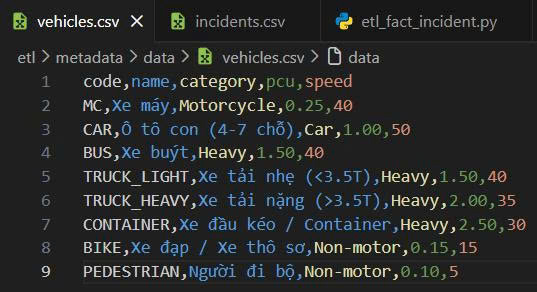
\includegraphics[width=0.7\textwidth]{Images/ETL_09}
    \vspace{6mm}
    \caption{Tệp cấu hình vehicles.csv chứa hệ số PCU và tốc độ thiết kế}
    \label{fig:etl_09}
\end{figure}

\paragraph{Phân loại mức độ nghiêm trọng thời tiết và sự cố}

Chuẩn hóa dữ liệu thô từ API về thang đo thống nhất qua các bảng \texttt{dim\_weather} và \texttt{dim\_incident\_type}.

\begin{description}
    \item[A. Danh mục Điều kiện Thời tiết (Weather Metadata):] \hfill \\
    Dữ liệu được phân loại theo \texttt{severity\_level} từ 1 (Bình thường) đến 4 (Cực đoan). Đi kèm các thuộc tính định tính được mã hóa: \texttt{visibility\_condition} và \texttt{road\_friction\_impact}.
    \item[B. Danh mục Loại hình Sự cố (Incident Metadata):] \hfill \\
    Phân nhóm logic vào các nhóm Tai nạn, Thi công, hoặc Ùn tắc. Đặc biệt tích hợp cột \texttt{color\_hex\_code} (ví dụ: \#FF0000 cho tai nạn) hỗ trợ hiển thị màu sắc biểu tượng trên bản đồ Dashboard một cách tự động.
\end{description}

\begin{figure}[htbp]
    \centering
    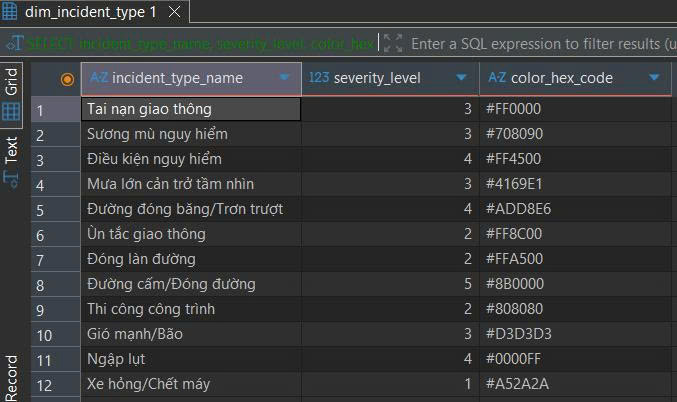
\includegraphics[width=0.9\textwidth]{Images/ETL_10}
    \vspace{6mm}
    \caption{Danh mục sự cố đã chuẩn hóa mã màu trong cơ sở dữ liệu}
    \label{fig:etl_10}
\end{figure}

\subsubsection{Nhóm chiều Hạ tầng Giao thông (Infrastructure Dimensions)}

Chiều hạ tầng giao thông được xác định là thành phần quan trọng nhất, đóng vai trò "xương sống" không gian (Spatial Backbone) của toàn bộ kho dữ liệu. Khác với các chiều dữ liệu định danh thông thường, nhóm này đòi hỏi quy trình xử lý phức tạp dựa trên lý thuyết đồ thị (Graph Theory) và các phép toán hình học không gian để chuyển đổi dữ liệu mạng lưới đường bộ từ OpenStreetMap (OSM) sang định dạng chuẩn của PostGIS. Việc xây dựng nhóm chiều này tuân thủ một trình tự phụ thuộc dữ liệu nghiêm ngặt để đảm bảo tính toàn vẹn tham chiếu: khởi tạo ranh giới hành chính, xây dựng nút giao và tuyến đường, sau đó phân rã thành các phân đoạn nhỏ (Segments).

\paragraph{Trích xuất ranh giới hành chính và Địa điểm (Location ETL)}

Quy trình nạp bảng \texttt{dim\_location} thực hiện định danh và số hóa ranh giới các vùng hành chính, tạo cơ sở cho việc phân tích lưu lượng giao thông theo từng địa phương.

\begin{description}
    \item[A. Kỹ thuật trích xuất dữ liệu không gian từ Overpass API] \hfill \\
    Hệ thống sử dụng thư viện chuyên dụng \texttt{OSMnx} để giao tiếp với API Overpass của OpenStreetMap.
    \begin{itemize}
        \item \textbf{Cơ chế truy vấn:} Gửi các yêu cầu truy vấn hướng đối tượng (Geocode-based requests) thay vì tải dữ liệu thô toàn bộ bản đồ.
        \item \textbf{Phân cấp hành chính:} Trích xuất đa tầng bao gồm Phường/Xã (Ward), Quận/Huyện (District) và Tỉnh/Thành phố (City).
        \item \textbf{Linh hoạt cấu hình:} Danh sách các khu vực trích xuất được tham số hóa để dễ dàng mở rộng phạm vi địa lý.
    \end{itemize}
\end{description}

\begin{figure}[htbp]
    \centering
    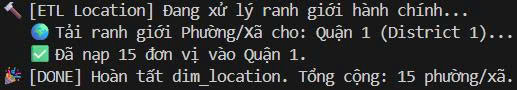
\includegraphics[width=0.7\textwidth]{Images/ETL_11}
    \vspace{6mm}
    \caption{Nhật ký thực thi nạp dữ liệu ranh giới hành chính Quận 1}
    \label{fig:etl_11}
\end{figure}

\begin{description}
    \item[B. Quy trình xử lý hình học (Geometry Processing)] \hfill \\
    Dữ liệu thô sau khi trích xuất cần trải qua các bước biến đổi hình học nghiêm ngặt để tương thích với cơ sở dữ liệu PostGIS:
    \begin{itemize}
        \item \textbf{Chuẩn hóa hệ tọa độ (CRS):} Ép buộc về hệ tọa độ WGS84 (EPSG:4326) để đảm bảo tính đồng nhất khi thực hiện các phép giao cắt không gian sau này.
        \item \textbf{Ép kiểu dữ liệu MULTIPOLYGON:} Lưu trữ dưới dạng \texttt{MULTIPOLYGON} để xử lý các vùng địa giới phức tạp bị chia cắt bởi sông ngòi hoặc hải đảo.
        \item \textbf{Tự động hóa mã hóa (Encoding):} Chuyển đổi đối tượng hình học sang định dạng Hex EWKB (Extended Well-Known Binary) thông qua thư viện \texttt{shapely}.
    \end{itemize}

    \item[C. Ràng buộc dữ liệu và Cơ chế bảo vệ (Data Integrity)] \hfill \\
    Để duy trì tính sạch của kho dữ liệu, hệ thống thiết lập các rào cản kỹ thuật:
    \begin{itemize}
        \item \textbf{Ràng buộc Unique phức hợp:} Thiết lập trên bộ ba cột (ward, district, city) để ngăn chặn trùng lặp bản ghi khi chạy lại quy trình ETL.
        \item \textbf{Chiến lược nạp dữ liệu:} Sử dụng mệnh đề \texttt{ON CONFLICT DO NOTHING} để tối ưu hóa thời gian và giữ nguyên các khóa ngoại đã tham chiếu.
        \item \textbf{Xây dựng mã vị trí (Location Code):} Tự động sinh \texttt{location\_code} chuẩn hóa (ví dụ: PHUONG\_BEN\_NGHE\_QUAN\_1) phục vụ tra cứu nhanh.
    \end{itemize}
\end{description}

\begin{figure}[htbp]
    \centering
    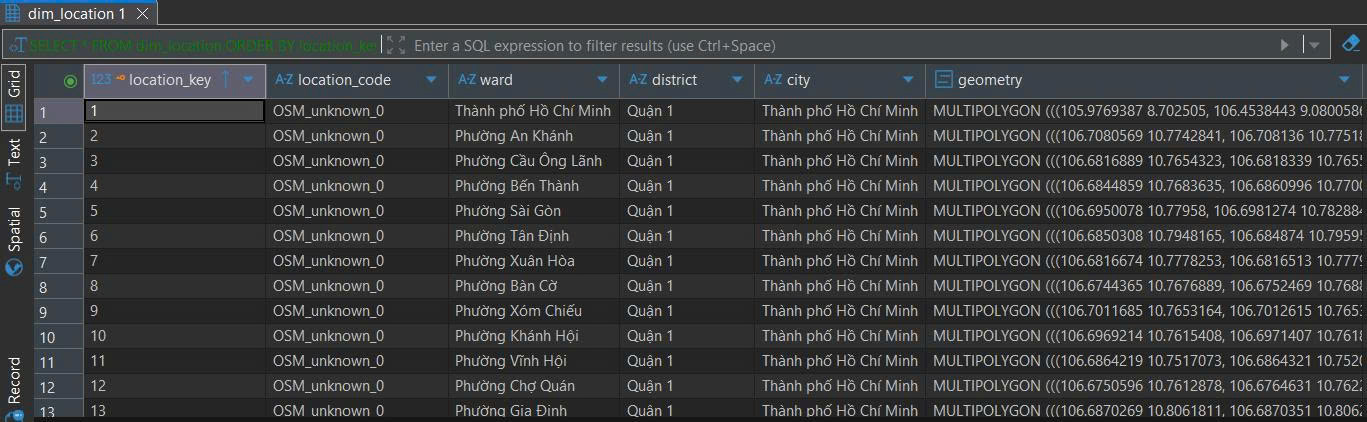
\includegraphics[width=0.9\textwidth]{Images/ETL_12}
    \vspace{6mm}
    \caption{Dữ liệu ranh giới hành chính đã nạp vào bảng dim\_location}
    \label{fig:etl_12}
\end{figure}

\begin{figure}[htbp]
    \centering
    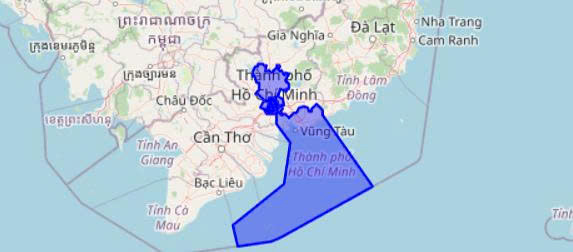
\includegraphics[width=0.5\textwidth]{Images/ETL_13}
    \vspace{6mm}
    \caption{Trực quan hóa đa giác ranh giới TP. Hồ Chí Minh từ PostGIS}
    \label{fig:etl_13}
\end{figure}

\paragraph{ Chuyển đổi mạng lưới đường bộ (Road, Way \& Node ETL)}

Quy trình này biến đổi đồ thị OSM thô thành các thực thể quản lý vật lý và logic.
\begin{itemize}
    \item \textbf{dim\_road (Tuyến đường):} Lưu trữ tên đường logic (ví dụ: Đường Điện Biên Phủ). Một Tuyến đường có thể bao gồm nhiều Đoạn đường vật lý khác nhau.
    \item \textbf{dim\_way (Đoạn đường vật lý):} Lưu trữ các đặc tính kỹ thuật như số làn xe (\texttt{lane\_count}), loại đường (\texttt{way\_type}), và giới hạn tốc độ thiết kế.
    \item \textbf{Số hóa Nút giao (Node ETL):} Toàn bộ các điểm giao cắt, quay đầu được trích xuất thành các bản ghi trong \texttt{dim\_node} dưới dạng một điểm (\texttt{POINT}) với tọa độ chính xác.
\end{itemize}

\paragraph{Phân đoạn và Tính toán hướng đường (Segment ETL)}

Phân đoạn đường (Segment ETL) là bước biến đổi dữ liệu phức tạp nhất, chuyển đổi cấu trúc đồ thị từ các thực thể đường dài (Ways) thành các đơn vị phân tích cơ sở gọi là Segments.

\begin{description}
    \item[A. Quy trình Segment hóa dựa trên cấu trúc đồ thị (Graph-based Segmenting)] \hfill \\
    Chia nhỏ mạng lưới dựa trên các điểm nút (Nodes) để quản lý vi mô các chỉ số giao thông chi tiết đến từng phân đoạn mét đường. Mỗi phân đoạn được cấp một \texttt{segment\_key} duy nhất.

    \item[B. Thuật toán tính toán Azimuth và vai trò trong Map Matching] \hfill \\
    Hướng di chuyển là thông tin sống còn để phân biệt dòng xe trên các đường hai chiều. Hệ thống tính góc hướng (Azimuth) tự động bằng công thức:
    \begin{itemize}
        \item $\Delta Lon = Lon_{to} - Lon_{from}$ 
        \item $\Delta Lat = Lat_{to} - Lat_{from}$ 
        \item $\theta = \operatorname{atan2}(\Delta Lon, \Delta Lat)$ 
    \end{itemize}
    Kết quả được chuẩn hóa về khoảng $[0^\circ, 360^\circ]$ để thực hiện kỹ thuật Map Matching, giúp đối khớp chính xác dữ liệu tốc độ thời gian thực từ TomTom API vào đúng hướng di chuyển tương ứng.

    \item[C. Chiến lược đa dạng hóa dữ liệu hình học (Dual-Geometry Strategy)] \hfill \\
    Mỗi Segment lưu trữ đồng thời hai loại dữ liệu không gian để tối ưu hóa hiển thị và hiệu năng xử lý:
    \begin{itemize}
        \item \textbf{geometry\_linestring (Chuỗi đường):} Lưu trữ tọa độ tạo nên hình dáng uốn lượn thực tế của đoạn đường, dùng để vẽ bản đồ nhiệt hoặc lộ trình.
        \item \textbf{geometry\_center (Điểm trung tâm):} Tính toán điểm trọng tâm (\texttt{Centroid}) của đoạn đường để tăng tốc các phép toán tìm kiếm lân cận hoặc giao cắt hành chính (Spatial Join).
    \end{itemize}
\end{description}

\begin{figure}[htbp]
    \centering
    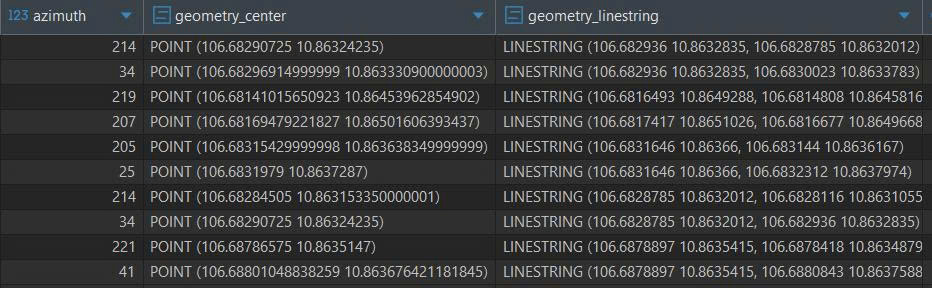
\includegraphics[width=1.0\textwidth]{Images/ETL_14}
    \vspace{6mm}
    \caption{Dữ liệu góc Azimuth và hình học đa tầng trong bảng dim\_segment}
    \label{fig:etl_14}
\end{figure}
\paragraph{Làm giàu dữ liệu bằng phép giao không gian (Spatial Enrichment)}

Sau khi hoàn tất việc nạp dữ liệu vào các bảng hạ tầng độc lập, kho dữ liệu vẫn tồn tại một khoảng cách giữa thực thể kỹ thuật (các phân đoạn đường OSM) và thực thể quản lý hành chính (Phường, Quận). Để giải quyết bài toán này, hệ thống triển khai bước "Enrichment" (Làm giàu dữ liệu) thông qua module \texttt{etl/infrastructure/etl\_enrichment.py}. Đây là quy trình hậu xử lý quan trọng nhằm thiết lập mối quan hệ logic giữa Hạ tầng và Hành chính một cách hoàn toàn tự động dựa trên tọa độ địa lý.

\begin{description}
    \item[A. Cơ chế Spatial Join thông qua hàm hình học PostGIS] \hfill \\
    Thay vì yêu cầu người dùng nhập liệu thủ công hoặc dựa vào các bảng tra cứu tĩnh dễ sai sót, hệ thống tận dụng sức mạnh xử lý không gian trực tiếp bên trong Database:
    \begin{itemize}
        \item \textbf{Thuật toán kiểm tra điểm trong đa giác (Point-in-Polygon):} Hệ thống thực thi các câu lệnh SQL sử dụng hàm \texttt{ST\_Contains} (hoặc \texttt{ST\_Within}) để đối chiếu hình học.
        \item \textbf{Quy trình xác định:} Quét qua toàn bộ các Segment có cột \texttt{location\_key} đang trống và xác định xem điểm trung tâm (\texttt{geometry\_center}) của đoạn đường đó nằm gọn trong đa giác ranh giới (\texttt{geometry}) nào của bảng \texttt{dim\_location}.
        \item \textbf{Tại sao sử dụng Điểm trung tâm (Geometry Center):} Một đoạn đường (\texttt{LineString}) có thể đi ngang qua ranh giới giữa hai phường, gây ra lỗi đa trùng lặp nếu thực hiện phép giao cắt toàn phần. Việc sử dụng điểm trung tâm giúp đảm bảo mỗi đoạn đường chỉ được gán duy nhất cho một đơn vị hành chính.
    \end{itemize}
\end{description}

\begin{figure}[htbp]
    \centering
    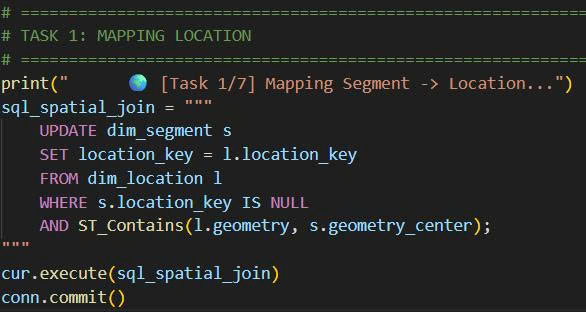
\includegraphics[width=0.8\textwidth]{Images/ETL_15}
    \vspace{6mm}
    \caption{Câu lệnh SQL thực hiện phép giao không gian để cập nhật location\_key}
    \label{fig:etl_15}
\end{figure}

\begin{description}
    \item[B. Tự động hóa cập nhật và tính nhất quán dữ liệu] \hfill \\
    Kết quả của phép giao không gian này là cột \texttt{location\_key} trong bảng \texttt{dim\_segment} được cập nhật giá trị tham chiếu chính xác đến bảng \texttt{dim\_location}. Nhờ có bước Enrichment này, mọi bản ghi Fact sau khi được gắn vào \texttt{segment\_key} sẽ nghiễm nhiên sở hữu thông tin hành chính thông qua mối quan hệ bắc cầu, hỗ trợ các báo cáo tổng hợp như "Tính toán tốc độ trung bình của toàn bộ các đoạn đường thuộc Quận 1" mà không cần can thiệp mã nguồn ETL.

    \item[C. Tối ưu hóa hiệu năng xử lý không gian (Spatial Indexing)] \hfill \\
    Do số lượng Segment có thể lên đến hàng chục nghìn bản ghi, hệ thống sử dụng \textbf{GIST Index} trên cột điểm trung tâm và chỉ mục không gian trên cột đa giác ranh giới của \texttt{dim\_location}. Điều này cho phép Database thực hiện phép giao không gian với độ phức tạp logarit thay vì quét toàn bộ bảng.
\end{description}

\subsection{QUY TRÌNH NẠP DỮ LIỆU SỰ KIỆN (FACT ETL PIPELINE)}

Quy trình nạp dữ liệu sự kiện (Fact ETL) là giai đoạn quan trọng nhất trong vận hành hàng ngày của hệ thống. Khác với dữ liệu Dimension mang tính chất tĩnh, dữ liệu Fact được thiết kế để thu thập các biến động không ngừng của mạng lưới giao thông theo thời gian thực (Real-time). Quy trình này thực hiện việc kết hợp dữ liệu từ các nguồn API quốc tế với dữ liệu quan trắc trực tiếp từ mô hình AI để tạo ra cái nhìn toàn diện về thực trạng giao thông.

\subsubsection{Tầng Dịch vụ thu thập dữ liệu (Data Service Layer)}

Để đảm bảo tính module hóa và dễ bảo trì, hệ thống tách biệt logic giao tiếp với các nhà cung cấp dữ liệu bên ngoài thành một tầng dịch vụ riêng biệt (\texttt{Service Layer}). Tầng này chịu trách nhiệm đóng gói các yêu cầu API, xử lý xác thực và chuẩn hóa dữ liệu thô (JSON) trước khi đưa vào các pipeline xử lý chính.

\begin{description}
    \item[a. Dịch vụ dữ liệu giao thông (TomTom Service)] \hfill \\
    Module \texttt{modules/tomtom\_service.py} là thành phần chịu trách nhiệm tương tác với TomTom:
    \begin{itemize}
        \item \textbf{Trích xuất dữ liệu lưu lượng (Traffic Flow):} Sử dụng endpoint \texttt{flowSegmentData} để truy vấn tốc độ di chuyển thực tế (\texttt{currentSpeed}) và tốc độ tự do (\texttt{freeFlowSpeed}) tại một tọa độ cụ thể.
        \item \textbf{Trích xuất dữ liệu sự cố (Traffic Incidents):} Sử dụng cơ chế quét theo vùng (Bounding Box) để lấy loại sự cố, tọa độ hình học, độ trễ và mô tả chi tiết sự việc.
    \end{itemize}
\end{description}

\begin{figure}[htbp]
    \centering
    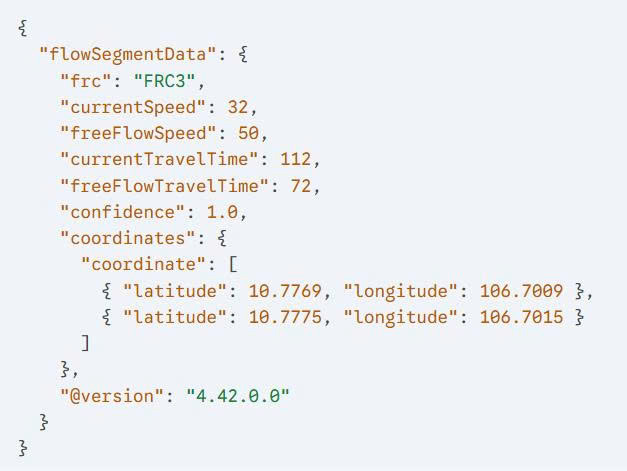
\includegraphics[width=0.6\textwidth]{Images/ETL_16}
    \vspace{6mm}
    \caption{Cấu trúc dữ liệu JSON trả về từ TomTom Traffic API}
    \label{fig:etl_16}
\end{figure}

\begin{description}
    \item[b. Dịch vụ dữ liệu khí tượng (Weather Service)] \hfill \\
    Dữ liệu thời tiết được cung cấp bởi module \texttt{modules/weather\_service.py} thông qua OpenWeatherMap API. Hệ thống thực hiện truy vấn theo tọa độ chính xác của từng đoạn đường (\textit{lat, lon}) để đảm bảo tính cục bộ, trả về các thông số: mã thời tiết (Weather ID), nhiệt độ, độ ẩm, tầm nhìn (\textit{visibility}) và lượng mưa.
\end{description}

\subsubsection{Tích hợp Thị giác máy tính trong quy trình ETL (AI Integration)}

Một điểm sáng tạo và đột phá của đồ án là việc tích hợp trực tiếp mô hình học sâu (Deep Learning) vào luồng xử lý dữ liệu Fact để thu thập số lượng phương tiện thực tế, thay vì chỉ dựa vào dữ liệu ước tính từ API.

\paragraph{ Kiến trúc bộ đếm phương tiện dựa trên YOLOv8}

Dự án triển khai module \texttt{modules/ai\_counter.py} để thu thập dữ liệu "ground truth" từ các nguồn camera giao thông trực tuyến.



\begin{description}
    \item[A. Lựa chọn mô hình YOLOv8x (Extra Large) cho độ chính xác tối ưu] \hfill \\
    Hệ thống sử dụng kiến trúc \textbf{YOLOv8} phiên bản "x" (Extra Large) cho độ chính xác cao nhất. Việc lựa chọn mô hình này là cần thiết để giải quyết bài toán mật độ phương tiện cực cao tại các nút giao thông TP.HCM, giúp nhận diện chính xác các đối tượng nhỏ như xe máy trong điều kiện bị che khuất (Occlusion).
\end{description}

\begin{figure}[htbp]
    \centering
    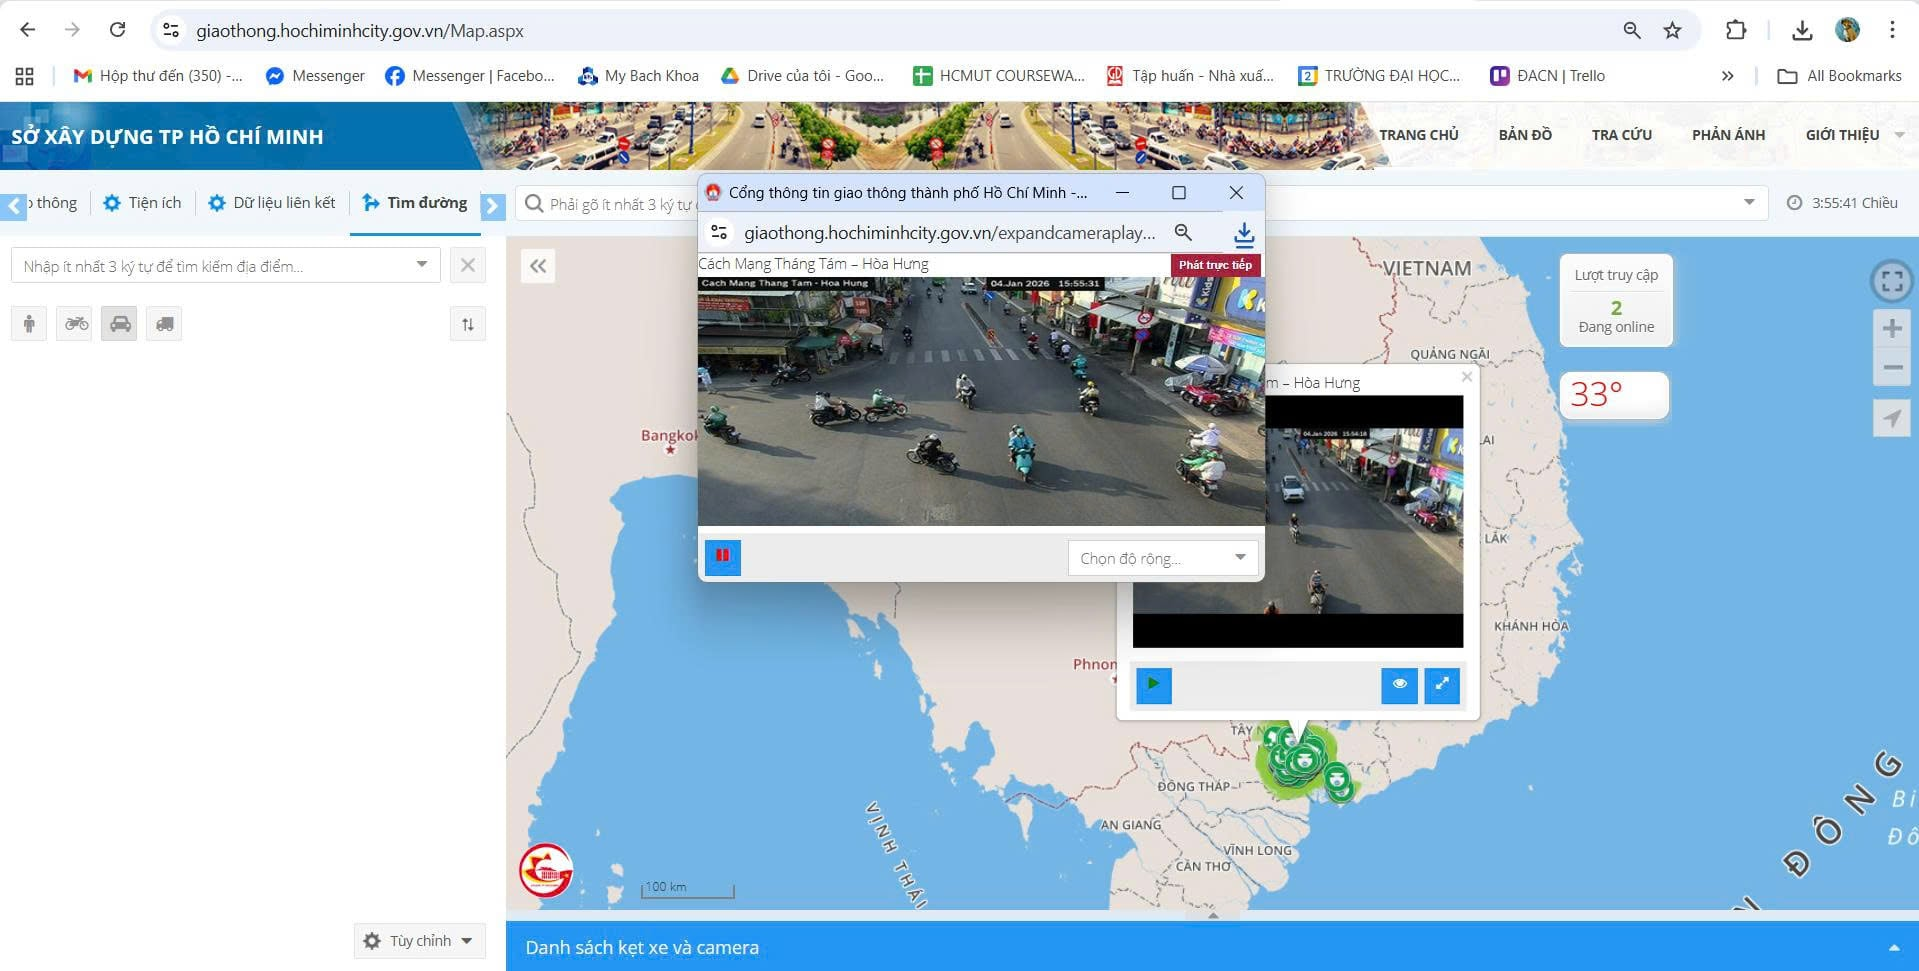
\includegraphics[width=1.0\textwidth]{Images/ETL_17a}
    \vspace{6mm}
    \caption{Trang web lấy hình ảnh camera tại Đường Cách Mạng Tháng Tám - Hòa Hưng}
    \label{fig:etl_17a}
\end{figure}

\begin{figure}[htbp]
    \centering
    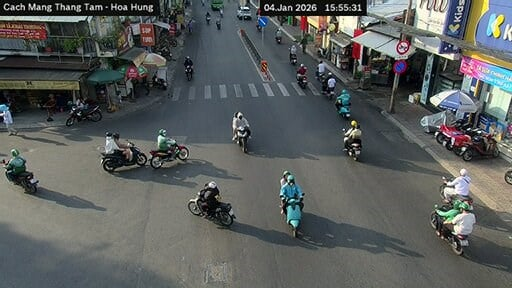
\includegraphics[width=1.0\textwidth]{Images/ETL_17b}
    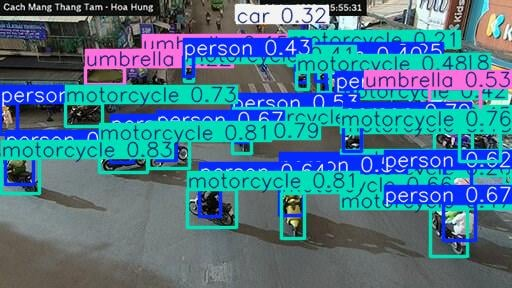
\includegraphics[width=1.0\textwidth]{Images/ETL_17}
    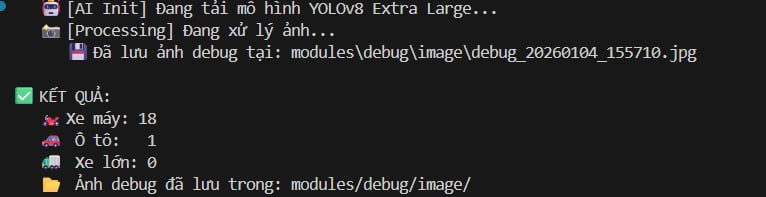
\includegraphics[width=1.0\textwidth]{Images/ETL_17c}
    \vspace{6mm}
    \caption{Kết quả nhận diện và phân lớp phương tiện thời gian thực bằng YOLOv8x}
    \label{fig:etl_17}
\end{figure}


\newpage
\begin{description}
    \item[B. Phân lớp đối tượng và Cơ chế lọc lớp (Class Filtering)] \hfill \\
    Hệ thống cấu hình \texttt{self.target\_classes = [2, 3, 5, 7]} để chỉ tập trung vào mảng giao thông:
    \begin{itemize}
        \item \textbf{Class 2 (Car):} Ánh xạ vào nhóm xe ô tô con.
        \item \textbf{Class 3 (Motorcycle):} Nhóm xe máy chiếm tỷ trọng lớn nhất tại Việt Nam.
        \item \textbf{Class 5 (Bus) và Class 7 (Truck):} Được gộp vào nhóm xe tải/xe hạng nặng (\texttt{heavy\_vehicle\_count}).
    \end{itemize}
    Các đối tượng nhiễu như người đi bộ, động vật hay biển báo đều bị bỏ qua ngay tại tầng xử lý AI.
\end{description}

\begin{figure}[htbp]
    \centering
    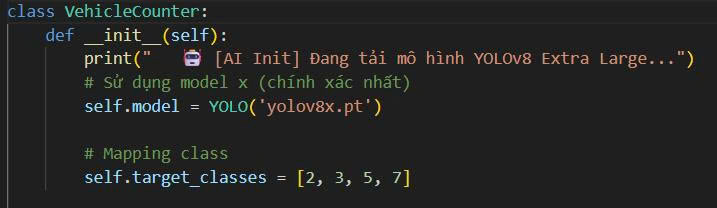
\includegraphics[width=0.8\textwidth]{Images/ETL_18}
    \vspace{6mm}
    \caption{Khởi tạo mô hình YOLOv8 và cấu hình danh mục đối tượng mục tiêu}
    \label{fig:etl_18}
\end{figure}
\paragraph{Quy trình chuẩn hóa dữ liệu AI và Tính toán lưu lượng quy đổi (PCU)}

Sau khi mô hình YOLOv8 hoàn tất việc phát hiện và gán nhãn các đối tượng trong khung hình, dữ liệu vẫn ở dạng danh sách các "Bounding Boxes" rời rạc. Quy trình ETL tiếp tục thực hiện bước chuẩn hóa dữ liệu và áp dụng các công thức nghiệp vụ để biến đổi chúng thành các chỉ số lưu lượng mang tính kỹ thuật.

\begin{description}
    \item[A. Cơ chế tổng hợp và Phân nhóm phương tiện (Aggregation Logic)] \hfill \\
    Hệ thống triển khai một hàm băm (Mapping Function) để chuyển đổi từ 80 lớp của tập dữ liệu COCO về 4 nhóm thực thể chính phù hợp với hạ tầng giao thông Việt Nam:
    \begin{itemize}
        \item \textbf{Nhóm xe máy (motorcycle\_count):} Được trích xuất trực tiếp từ class ID 3. Đây là nhóm đối tượng có kích thước nhỏ và mật độ dày đặc nhất, đòi hỏi độ chính xác cao trong nhận diện.
        \item \textbf{Nhóm xe con (car\_count):} Trích xuất từ class ID 2.
        \item \textbf{Nhóm xe hạng nặng (heavy\_vehicle\_count):} Hệ thống thực hiện phép hợp (Union) các đối tượng thuộc class 5 (Bus) và class 7 (Truck). Việc gộp nhóm này giúp đơn giản hóa bài toán tính toán tải trọng lên mặt đường.
        \item \textbf{Nhóm phương tiện khác (other\_count):} Bao gồm các lớp như xe đạp, xe lôi hoặc các phương tiện không xác định khác để đảm bảo không bỏ sót bất kỳ thực thể nào đang chiếm dụng không gian đường bộ.
    \end{itemize}

    \item[B. Thuật toán tính toán lưu lượng quy đổi (PCU Calculation)] \hfill \\
    Để đánh giá chính xác mức độ tắc nghẽn, hệ thống quy đổi số lượng xe về đơn vị xe con tiêu chuẩn (Passenger Car Unit - PCU). Công thức được cài đặt trực tiếp trong module \texttt{ai\_counter.py} dựa trên các hệ số thực nghiệm:
    \begin{equation}
        Total\_PCU = N_{moto} \times 0.25 + N_{car} \times 1.0 + N_{heavy} \times 2.0 + N_{other} \times 1.0
    \end{equation}
    Việc sử dụng hệ số 0.25 cho xe máy phản ánh thực tế rằng diện tích chiếm dụng động của một xe máy chỉ bằng 1/4 so với một xe ô tô con tiêu chuẩn. Chỉ số \texttt{total\_pcu} là dữ liệu đầu vào quan trọng nhất để tính toán mật độ dòng chảy và khả năng thông hành của đoạn đường.
\end{description}

\begin{figure}[htbp]
    \centering
    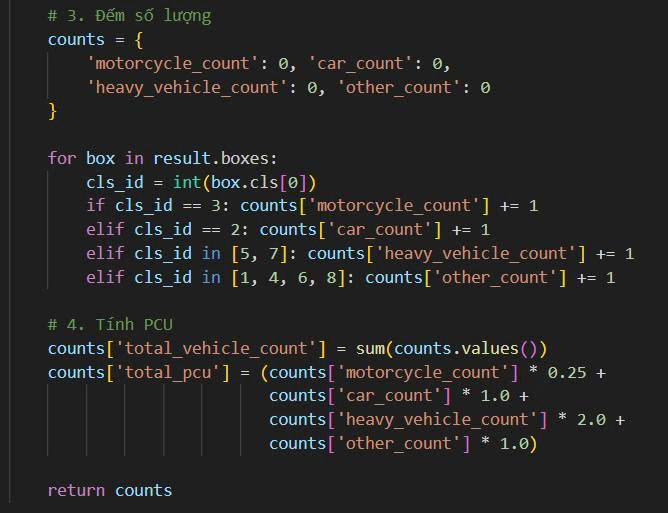
\includegraphics[width=0.8\textwidth]{Images/ETL_19}
    \vspace{6mm}
    \caption{Đoạn mã triển khai logic đếm đối tượng và tính toán PCU từ kết quả AI}
    \label{fig:etl_19}
\end{figure}

\subsubsection{Xác định chỉ số LOS (Level of Service) và Mức độ ùn tắc}

Từ dữ liệu AI và vận tốc thu thập được, hệ thống tiến hành phân loại chất lượng dòng lưu lượng thông qua chỉ số LOS (A-F) ngay trong module \texttt{etl\_fact\_traffic.py}:

\begin{itemize}
    \item \textbf{Công thức tính Congestion Level:} Hệ thống so sánh tốc độ thực tế (\texttt{current\_speed}) với tốc độ tự do (\texttt{free\_flow\_speed}) để tính toán tỷ lệ phần trăm ùn tắc.
    \item \textbf{Phân cấp LOS:}
    \begin{itemize}
        \item \textbf{LOS A/B:} Dòng xe lưu thông tự do, tốc độ thực tế gần bằng tốc độ thiết kế (Congestion $<$ 15\%).
        \item \textbf{LOS C/D:} Dòng xe bắt đầu bị ảnh hưởng, người lái khó thay đổi làn đường (Congestion 15\% - 45\%).
        \item \textbf{LOS E/F:} Dòng xe bị ùn tắc nghiêm trọng hoặc đứng im, tốc độ giảm sâu (Congestion $>$ 45\%).
    \end{itemize}
    \item \textbf{Ghi nhận dữ liệu:} Toàn bộ các chỉ số này được đóng gói thành một bản ghi và đẩy vào phân vùng tương ứng của bảng \texttt{fact\_traffic\_flow}.
\end{itemize}

\begin{figure}[htbp]
    \centering
    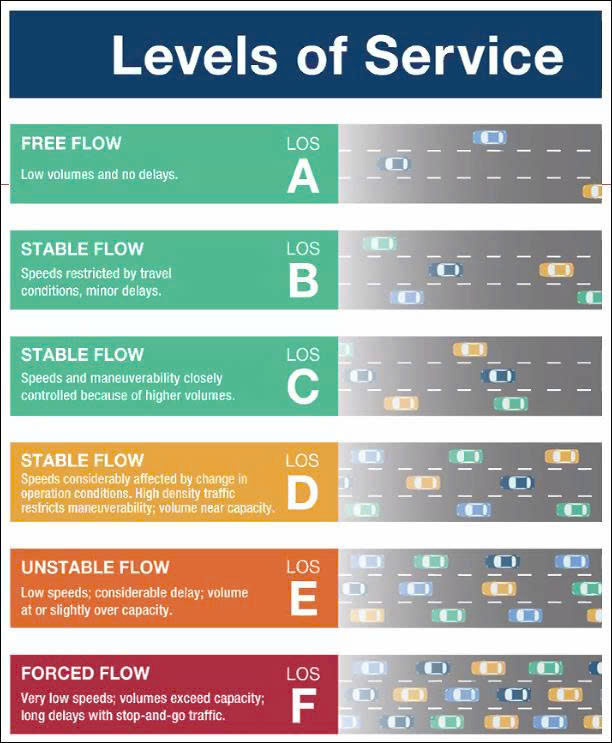
\includegraphics[width=0.6\textwidth]{Images/ETL_20}
    \vspace{6mm}
    \caption{Mô tả các cấp độ phục vụ (LOS) trong kỹ thuật giao thông}
    \label{fig:etl_20}
\end{figure}

\subsubsection{ Quy trình nạp dữ liệu Fact Traffic Flow và Fact Incident}

Các bảng Fact là trái tim của Star Schema, lưu trữ các chỉ số định lượng về trạng thái mạng lưới giao thông. Quy trình nạp dữ liệu vào bảng Fact yêu cầu sự kết hợp phức tạp giữa các kỹ thuật đối khớp không gian (Spatial Matching) và logic nghiệp vụ để đảm bảo tính nhất quán giữa dữ liệu động và hạ tầng tĩnh.

\paragraph{ Quy trình nạp dữ liệu Lưu lượng Giao thông (Fact Traffic Flow ETL)}

Đây là quy trình quan trọng nhất trong hệ thống, thực hiện nhiệm vụ tổng hợp và đồng bộ hóa dữ liệu từ ba nguồn khác nhau: Trí tuệ nhân tạo (AI), API Giao thông (TomTom) và API Thời tiết (OpenWeatherMap) thành một bản ghi thông tin duy nhất đại diện cho trạng thái của một phân đoạn đường tại một thời điểm cụ thể.

\begin{description}
    \item[A. Cơ chế Hợp nhất dữ liệu đa nguồn (Multi-source Data Fusion)] \hfill \\
    Hệ thống tập trung vào các vị trí chiến lược được định nghĩa trong cấu hình \texttt{CAMERA\_MAPPING}. Pipeline thực hiện quét qua danh sách các \texttt{segment\_key} có gắn camera giám sát. Với mỗi Segment, hệ thống đóng vai trò như một bộ não trung tâm, kích hoạt đồng thời hai luồng thu thập dữ liệu:
    \begin{itemize}
        \item \textbf{Luồng quan trắc mật độ (AI Stream):} Gọi module \texttt{ai\_counter.py} để phân tích ảnh camera, trả về số lượng chi tiết từng loại xe và tổng lưu lượng quy đổi PCU.
        \item \textbf{Luồng quan trắc vận tốc (API Stream):} Gọi \texttt{tomtom\_service.py} để lấy tốc độ di chuyển thực tế và tốc độ tự do tại đúng tọa độ của phân đoạn đó.
    \end{itemize}
    Việc kết hợp giữa "Mật độ" (từ AI) và "Vận tốc" (từ API) cho phép hệ thống xây dựng được biểu đồ quan hệ cơ bản của dòng giao thông (Fundamental Diagram of Traffic Flow).

    \item[B. Quy trình xác định khóa tham chiếu và Liên kết ngữ cảnh (Key Mapping)] \hfill \\
    Để dữ liệu Fact có thể liên kết được với các bảng Dimension, hệ thống thực hiện ánh xạ khóa nghiêm ngặt:
    \begin{itemize}
        \item \textbf{Khóa thời gian (Temporal Keys):} Thời gian thực thi được băm nhỏ thành \texttt{time\_key} (phút trong ngày) và \texttt{date\_key} (YYYYMMDD) để thực hiện các phép Join cực nhanh bằng kiểu dữ liệu Integer.
        \item \textbf{Khóa ngữ cảnh thời tiết (Weather Key):} Tại mỗi vị trí camera, hệ thống gọi dịch vụ thời tiết để ghi nhận điều kiện khí tượng tức thời. Mã thời tiết trả về được ánh xạ thành \texttt{weather\_key}, hỗ trợ phân tích tương quan giữa thời tiết và lưu lượng xe.
    \end{itemize}
\end{description}

\begin{figure}[htbp]
    \centering
    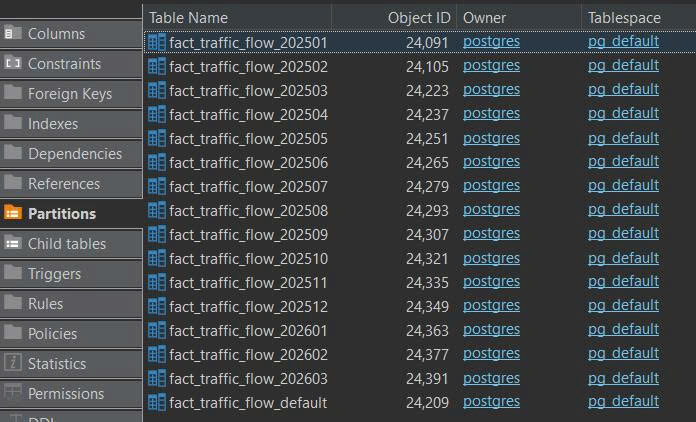
\includegraphics[width=0.8\textwidth]{Images/ETL_21}
    \vspace{6mm}
    \caption{Cấu trúc các phân vùng bảng Fact theo tháng trong PostgreSQL}
    \label{fig:etl_21}
\end{figure}

\begin{description}
    \item[C. Tính toán chỉ số hiệu suất và Phân cấp LOS (Performance Metrics)] \hfill \\
    Sau khi hợp nhất dữ liệu, hệ thống tính toán \texttt{congestion\_level} dựa trên tỷ lệ giữa tốc độ hiện tại và tốc độ tự do. Hệ thống áp dụng bộ quy tắc phân loại LOS từ A đến F để đánh giá chất lượng dịch vụ. Toàn bộ bản ghi được nạp theo lô (Batch Load) vào Database thông qua hàm \texttt{executemany} để tối ưu hóa hiệu năng ghi.
\end{description}

\begin{figure}[htbp]
    \centering
    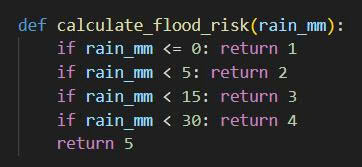
\includegraphics[width=0.8\textwidth]{Images/ETL_22}
    \vspace{6mm}
    \caption{Hàm xử lý logic tính toán chỉ số rủi ro ngập lụt}
    \label{fig:etl_22}
\end{figure}
\paragraph{ Quy trình nạp dữ liệu Sự cố Giao thông (Fact Incident ETL)}

Bảng \texttt{fact\_incident} đóng vai trò lưu trữ các sự kiện bất thường gây ảnh hưởng đến năng lực thông hành của mạng lưới đường bộ như tai nạn, thi công, hoặc thời tiết cực đoan. Quy trình ETL cho bảng này, được triển khai trong module \texttt{etl/fact/etl\_fact\_incident.py}, giải quyết bài toán thách thức về đối khớp một điểm tọa độ sự cố tự do vào một đoạn đường quản lý cụ thể (Point-to-Segment Mapping).

\begin{description}
    \item[A. Thuật toán Tìm kiếm phân đoạn gần nhất (Spatial Lookup) dựa trên Haversine] \hfill \\
    Dữ liệu sự cố từ TomTom API trả về dưới dạng tọa độ kinh/vĩ độ (\texttt{Point}). Tuy nhiên, để dữ liệu này có giá trị phân tích, sự cố phải được gắn (\texttt{Link}) chính xác với một \texttt{segment\_key} trong kho dữ liệu.
    \begin{itemize}
        \item \textbf{Tính toán khoảng cách địa cầu:} Do PostGIS thực hiện các phép tính trên mặt cầu, hệ thống triển khai hàm \texttt{calculate\_distance\_haversine} để đo khoảng cách chính xác theo đường chim bay giữa vị trí sự cố và điểm trung tâm (\texttt{geometry\_center}) của từng đoạn đường.
        \item \textbf{Công thức áp dụng:} Hệ thống sử dụng bán kính Trái đất $R = 6,371,000$ mét và các phép tính lượng giác để xác định khoảng cách chính xác đến từng mét.
        \item \textbf{Chiến lược lựa chọn đối tượng:} Hệ thống thực hiện quét trong bán kính lân cận (dưới 50m - 100m) để tìm phân đoạn phù hợp nhất. Nếu sự cố nằm quá xa các đoạn đường đã số hóa (vượt ngưỡng sai số GPS), hệ thống sẽ tự động ghi nhận vào log và bỏ qua (\texttt{skipped\_count}) để đảm bảo tính sạch của dữ liệu.
    \end{itemize}

    \item[B. Cơ chế Ánh xạ loại sự cố (Incident Type Mapping)] \hfill \\
    TomTom sử dụng hệ thống mã số riêng để định danh loại sự kiện. Hệ thống ETL thực hiện bước chuẩn hóa dữ liệu thông qua từ điển ánh xạ \texttt{TOMTOM\_INCIDENT\_MAP}:
    \begin{itemize}
        \item \textbf{Đồng nhất hóa danh mục:} Mọi sự cố từ API được chuyển đổi sang các mã chuẩn như \texttt{ACCIDENT}, \texttt{ROAD\_WORK}, \texttt{FLOOD}... đã được định nghĩa trong bảng \texttt{dim\_incident\_type}.
        \item \textbf{Tích hợp bối cảnh khí tượng:} Ngay khi một sự cố được ghi nhận, hệ thống đồng thời gọi \texttt{get\_weather\_by\_coords} để lấy thông tin thời tiết tại thời điểm đó, hỗ trợ phân tích các yếu tố tác động ngoại cảnh.
    \end{itemize}

    \item[C. Cấu trúc nạp dữ liệu và Quản lý dòng thời gian (Loading \& Timeline)] \hfill \\
    Dữ liệu sự cố được nạp với đầy đủ các thuộc tính: ghi nhận thời gian tồn tại (\texttt{start\_time} và \texttt{expected\_end\_time}) để tính toán tổng thời gian ảnh hưởng; ghi nhận chỉ số tác động (\texttt{delay\_seconds} và \texttt{length\_meters}). Hệ thống sử dụng kỹ thuật \texttt{Batch Insert} để nạp một lần duy nhất vào PostgreSQL, giúp giảm độ trễ và tránh tình trạng khóa bảng.
\end{description}

\begin{figure}[htbp]
    \centering
    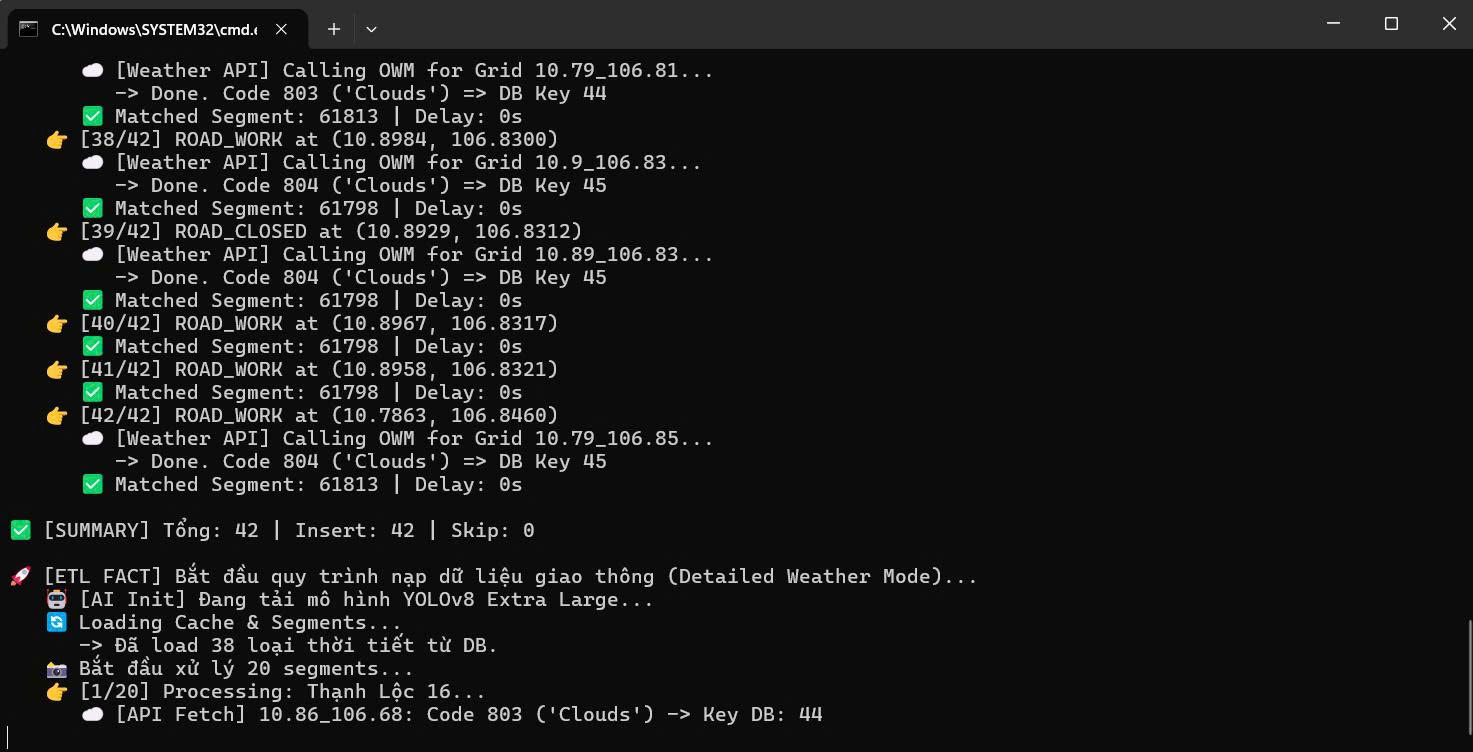
\includegraphics[width=0.8\textwidth]{Images/ETL_23}
    \vspace{6mm}
    \caption{Nhật ký nạp dữ liệu sự cố và kết quả đối khớp không gian thành công}
    \label{fig:etl_23}
\end{figure}

\paragraph{Chiến lược Quản trị Phân vùng và Hiệu năng (Partitioning \& Performance)}

Với tần suất nạp dữ liệu 15 phút/lần, các bảng Fact sẽ nhanh chóng tích lũy hàng triệu bản ghi. Để đảm bảo hệ thống không bị suy giảm hiệu năng, dự án triển khai các kỹ thuật quản trị dữ liệu quy mô lớn ngay từ tầng vật lý.

\begin{description}
    \item[A. Kỹ thuật Phân vùng dữ liệu theo dải thời gian (Range Partitioning)] \hfill \\
    Áp dụng tính năng \texttt{Declarative Partitioning} cho bảng \texttt{fact\_traffic\_flow}. Dữ liệu được phân tán vào các bảng con dựa trên giá trị của \texttt{date\_key} theo từng tháng (ví dụ: \texttt{fact\_traffic\_flow\_202501}). Việc này giúp tránh hiện tượng "Bloat" dữ liệu, giảm chi phí bảo trì chỉ mục và cho phép thực hiện cơ chế \texttt{Partition Pruning} khi truy vấn, giúp tăng tốc độ phản hồi đáng kể.

    \item[B. Tối ưu hóa hệ thống chỉ mục đa tầng (Multi-level Indexing)] \hfill \\
    Thiết lập chỉ mục \texttt{B-Tree} trên các khóa ngoại (\texttt{segment\_key}, \texttt{time\_key}, \texttt{date\_key}) để tối ưu các phép toán \texttt{JOIN}. Đặc biệt, chỉ mục không gian \texttt{GIST} được đánh trên cột \texttt{geometry} của bảng \texttt{fact\_incident}, cho phép thực hiện các truy vấn phức tạp như tìm kiếm sự cố trong bán kính người dùng hoặc vẽ bản đồ nhiệt (\texttt{Heatmap}) với độ phức tạp logarit.

    \item[C. Lợi ích tổng thể về vận hành] \hfill \\
    Đảm bảo thời gian chạy của mỗi batch ETL luôn ổn định dưới 2 phút. Đồng thời, dễ dàng thực hiện việc lưu trữ (\texttt{Archiving}) hoặc xóa dữ liệu cũ bằng cách ngắt kết nối (\texttt{Detach}) một phân vùng tháng mà không làm gián đoạn hệ thống đang chạy.
\end{description}

\begin{figure}[htbp]
    \centering
    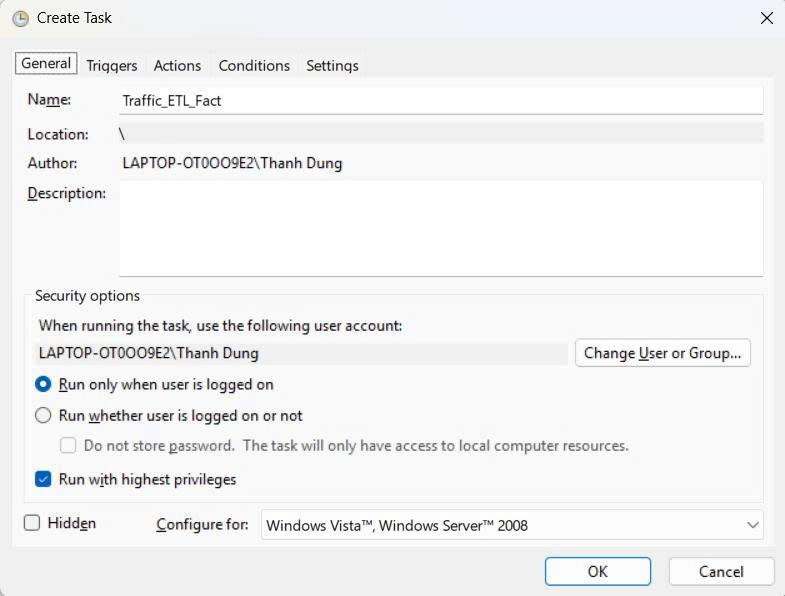
\includegraphics[width=0.8\textwidth]{Images/ETL_24}
    \vspace{6mm}
    \caption{Giao diện Task Scheduler}
    \label{fig:etl_24}
\end{figure}

\paragraph{ Xử lý nạp dữ liệu Tác động Thời tiết (Fact Weather Impact ETL)}

Module \texttt{etl/fact/etls\_fact\_weather\_impact.py} được thiết kế để thực hiện các phép phân tích phái sinh nhằm định lượng hóa mức độ ảnh hưởng của thời tiết lên năng lực vận hành và độ an toàn của từng đoạn đường.

\begin{description}
    \item[A. Thuật toán tính toán chỉ số rủi ro (Risk Scoring Algorithm)] \hfill \\
    Hệ thống triển khai các mô hình toán học để chuyển đổi đơn vị vật lý thành thang điểm rủi ro từ 0 đến 100:
    \begin{itemize}
        \item \textbf{Chỉ số rủi ro ngập lụt (\textit{Flood\_Risk\_Score}):} Tính toán dựa trên lượng mưa tức thời ($P_{1h}$), hệ số tác động địa hình ($I_{factor}$) và năng lực thoát nước ($D_{capacity}$):
        \begin{equation}
            Flood\_Risk = \min \left( 100, \frac{P_{1h} \times I_{factor}}{D_{capacity}} \times 100 \right)
        \end{equation}
        \item \textbf{Chỉ số an toàn tầm nhìn (\textit{Visibility\_Safety\_Score}):} Đánh giá dựa trên trường \texttt{visibility}. Tầm nhìn dưới 500m kích hoạt cảnh báo nguy hiểm (\texttt{Danger}), trong khi tầm nhìn trên 2000m được coi là an toàn.
    \end{itemize}

    \item[B. Logic đối khớp không gian và làm giàu dữ liệu] \hfill \\
    Dữ liệu tác động thời tiết được gắn trực tiếp vào \texttt{segment\_key} dựa trên tọa độ trung tâm, cho phép nhận diện các "điểm đen" về ngập lụt trên từng con phố cụ thể. Đồng thời, hệ thống sử dụng bộ quy tắc logic (\texttt{Knowledge Base}) để suy diễn trạng thái mặt đường (Khô ráo, Trơn trượt, Ngập nước) dựa trên mã thời tiết.

    \item[C. Ý nghĩa đối với bài toán phân tích đa chiều] \hfill \\
    Cho phép thực hiện phép \texttt{JOIN} giữa \texttt{fact\_traffic\_flow} và \texttt{fact\_weather\_impact} để tìm ra hệ số giảm tốc độ trung bình của xe máy khi trời mưa, cung cấp dữ liệu nền tảng cho các thuật toán dự báo tắc nghẽn.
\end{description}

\begin{figure}[htbp]
    \centering
    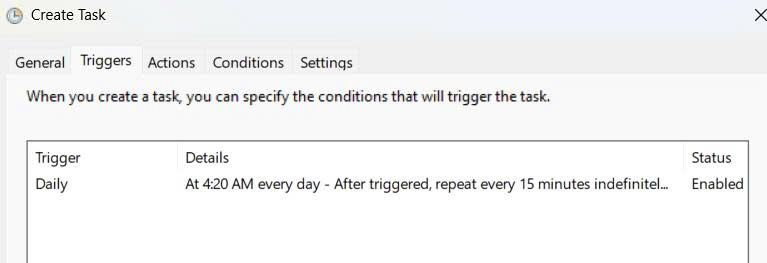
\includegraphics[width=0.5\textwidth]{Images/ETL_25}
    \vspace{6mm}
    \caption{Set up Trigger theo lịch ETL}
    \label{fig:etl_25}
\end{figure}
\subsubsection{ Quy trình giả lập dữ liệu (Mock Data Pipeline)}

Trong giai đoạn phát triển và tối ưu hóa kho dữ liệu, việc chỉ phụ thuộc vào dữ liệu thời gian thực từ API là chưa đủ để kiểm chứng các mô hình phân tích dài hạn hoặc kiểm thử hiệu năng truy vấn trên quy mô lớn. Do đó, hệ thống triển khai một Pipeline chuyên biệt để giả lập dữ liệu (Mock Data) thông qua module \texttt{pipelines/run\_all\_mocks.py}. Quy trình này mô phỏng các thực thể người dùng, hành vi di chuyển và hiệu suất hạ tầng dựa trên các quy luật xác suất thực tế.

\paragraph{ Giả lập thực thể Người dùng (User Mocking)}

Module \texttt{etl/mock/etl\_mock\_user.py} thực hiện khởi tạo tập khách hàng giả lập cho hệ thống:
\begin{itemize}
    \item \textbf{Tạo dữ liệu định danh:} Sử dụng thư viện \texttt{Faker} để sinh ra các thông tin như tên người dùng, số điện thoại và email đảm bảo tính duy nhất và định dạng chuẩn.
    \item \textbf{Quản lý trạng thái:} Mỗi người dùng được gán các thuộc tính như ngày đăng ký (\texttt{created\_at}) lùi về quá khứ để tạo ra tập dữ liệu có chiều sâu thời gian, phục vụ cho các báo cáo về tăng trưởng người dùng (User Growth).
    \item \textbf{Nạp dữ liệu:} Toàn bộ dữ liệu được đẩy vào bảng \texttt{dim\_user} thông qua kỹ thuật \texttt{Batch Insert} để tối ưu tốc độ.
\end{itemize}

\paragraph{ Mô phỏng hành trình di chuyển (Trip Mocking)}

Đây là phần phức tạp nhất trong quy trình giả lập, thực hiện tại \texttt{etl/mock/etl\_mock\_trip.py} để nạp dữ liệu vào bảng \texttt{fact\_trip}:
\begin{itemize}
    \item \textbf{Logic chọn lộ trình:} Hệ thống thực hiện lấy ngẫu nhiên các cặp \texttt{segment\_key} từ bảng \texttt{dim\_segment} để làm điểm bắt đầu và điểm kết thúc của một chuyến đi.
    \item \textbf{Tính toán thông số chuyến đi:}
    \begin{itemize}
        \item \textbf{Khoảng cách ($d$):} Được tính toán dựa trên độ dài thực tế của các phân đoạn đường được chọn.
        \item \textbf{Thời gian di chuyển ($t$):} Được suy diễn từ vận tốc trung bình của loại xe (\texttt{avg\_speed} trong \texttt{dim\_vehicle\_type}) cộng thêm một sai số ngẫu nhiên (\textit{Random Variance}) để mô phỏng tình trạng giao thông biến động.
    \end{itemize}
    \item \textbf{Tiêu hao nhiên liệu và Khí thải:} Hệ thống áp dụng các công thức ước tính để sinh dữ liệu cho cột \texttt{fuel\_consumed\_liters} và \texttt{co2\_emitted\_kg}, hỗ trợ cho các bài toán phân tích môi trường.
\end{itemize}

\paragraph{ Giả lập Hiệu suất Phân đoạn lịch sử (Segment Performance Mocking)}

Để Dashboard có thể hiển thị các biểu đồ so sánh theo năm/tháng, module \texttt{etl/mock/etl\_mock\_segment\_performance.py} thực hiện nạp dữ liệu lịch sử giả định cho bảng \texttt{fact\_segment\_performance}:
\begin{itemize}
    \item \textbf{Tạo dữ liệu Baseline:} Hệ thống lấy dữ liệu vận tốc thiết kế từ \texttt{dim\_way} làm mốc chuẩn.
    \item \textbf{Mô phỏng chu kỳ thời gian:} Dữ liệu được sinh ra theo quy luật: giảm tốc độ vào các khung giờ cao điểm (Morning/Afternoon Shifts) và tăng tốc độ vào ban đêm.
    \item \textbf{Lợi ích:} Việc này giúp kiểm thử tính đúng đắn của các câu lệnh SQL Aggregate phức tạp trước khi có đủ dữ liệu thực tế sau nhiều tháng vận hành.
\end{itemize}

\subsection{TỰ ĐỘNG HÓA VÀ GIÁM SÁT VẬN HÀNH (AUTOMATION \& MONITORING)}

Để đảm bảo kho dữ liệu luôn phản ánh trạng thái mới nhất của mạng lưới giao thông mà không cần sự can thiệp thủ công từ quản trị viên, dự án đã triển khai một hệ thống vận hành tự động hóa hoàn toàn. Cơ chế này chuyển đổi các kịch bản xử lý dữ liệu đơn lẻ thành một chu kỳ sống liên tục, đáp ứng tiêu chuẩn của một hệ thống Real-time Data Warehouse.

\subsubsection{ Cơ chế vận hành thông qua Batch Script và Điều phối hệ thống}

Tệp kịch bản \texttt{scripts/run\_etl\_fact\_daily.bat} đóng vai trò là lớp vỏ điều phối (\textit{Wrapper}) bên ngoài, giúp kết nối mã nguồn Python với hệ điều hành Windows.

\paragraph{ Tự động hóa quản lý môi trường thực thi (Virtual Environment Activation)}

Batch script thực hiện kích hoạt môi trường cô lập bằng lệnh \texttt{call .venv\textbackslash Scripts\textbackslash activate}. Điều này đảm bảo rằng mọi thư viện quan trọng như \texttt{ultralytics}, \texttt{psycopg2} và \texttt{OSMnx} luôn được chạy đúng phiên bản đã kiểm thử, loại bỏ hoàn toàn các lỗi thiếu Module khi chạy tự động.

\begin{figure}[htbp]
\centering
\begin{minipage}{0.9\textwidth}
\begin{verbatim}
@echo off
setlocal enabledelayedexpansion
chcp 65001 > nul
cd /d "C:\Path\To\Project\project_folder"
if not exist "logs" mkdir "logs"
call .venv\Scripts\activate
echo [START] ETL JOB STARTED AT %TIME%
powershell -Command "python -u main_etl.py --mode fact 2>&1 | Tee-Object ..."
pause
\end{verbatim}
\end{minipage}
\vspace{6mm}
\caption{Cấu trúc tệp lệnh Batch thực thi chu kỳ ETL tự động}
\label{fig:etl_26}
\end{figure}

\paragraph{ Chiến lược lập lịch chu kỳ (Windows Task Scheduler Integration)}

Dự án tận dụng Windows Task Scheduler làm "nhịp đập" cho toàn hệ thống với tần suất thực thi 15 phút một lần. Đây là khoảng thời gian tối ưu để cân bằng giữa độ trễ dữ liệu và hạn mức API miễn phí. Cấu hình "Run whether user is logged on or not" đảm bảo quy trình ETL vẫn diễn ra ngầm định ngay cả khi không có người dùng đăng nhập.

\paragraph{ Tối ưu hóa tham số và Quản lý tài nguyên}

Việc sử dụng tham số \texttt{--mode fact} giúp hệ thống chỉ tập trung vào các bảng dữ liệu biến động, giảm thời gian thực thi mỗi Batch xuống dưới 3 phút, từ đó giải phóng tài nguyên CPU/GPU cho các tác vụ khác.

\subsubsection{ Hệ thống ghi nhật ký tập trung (Logging System)}

Hệ thống triển khai cơ chế \textit{Centralized Logging} dựa trên thư viện \texttt{logging} tiêu chuẩn của Python.

\begin{itemize}
    \item \textbf{Tiêu chuẩn hóa cấu trúc nhật ký:} Sử dụng định dạng \texttt{[Thời gian] - [Tên Module] - [Cấp độ] - [Thông điệp]}. Nhật ký được ghi song song ra màn hình console và tệp tin \texttt{.log} để phục vụ tra cứu.
    \item \textbf{Giám sát sức khỏe Pipeline (Health Monitoring):} Nhật ký ghi lại chi tiết số lượng bản ghi nạp thành công, số lượng bị lỗi (\textit{Skip}) và tổng thời gian thực thi, giúp đánh giá độ bao phủ dữ liệu (\textit{Data Coverage}).
    \item \textbf{Quản lý ngoại lệ (Exception Handling):} Hệ thống bắt các ngoại lệ cụ thể (như \texttt{psycopg2.Error}) và ghi lại \textit{Error Traceback}, giúp quản trị viên phân biệt lỗi do hạ tầng hay lỗi từ API bên thứ ba.
\end{itemize}

\begin{figure}[htbp]
    \centering
    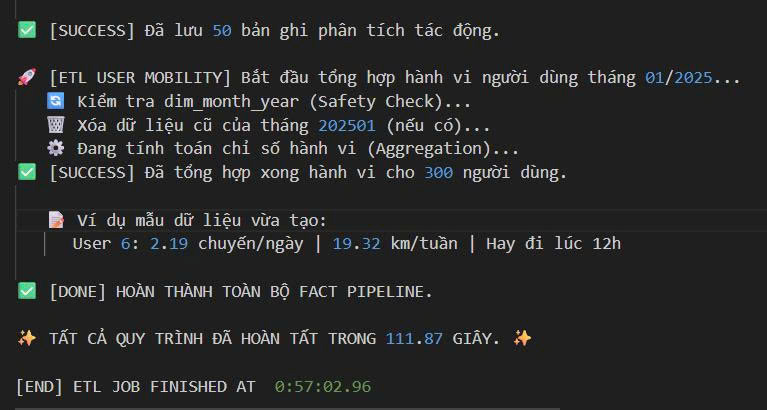
\includegraphics[width=0.9\textwidth]{Images/ETL_27}
    \vspace{6mm}
    \caption{Nhật ký tổng hợp kết thúc quy trình Fact Pipeline thành công}
    \label{fig:etl_27}
\end{figure}

\subsection{Kết chương}

Chương 8 đã trình bày một cách toàn diện quy trình xây dựng hệ thống ETL – trung tâm điều phối của kho dữ liệu giao thông thông minh. Chương này đã đạt được các kết quả kỹ thuật then chốt:

\begin{itemize}
    \item \textbf{Kiến trúc đa tầng bền vững:} Hiện thực hóa mô hình điều phối từ \texttt{main\_etl.py} đến các pipeline nguyên tử, tối ưu hóa tài nguyên và quản lý lỗi tập trung.
    \item \textbf{Chuẩn hóa Không gian - Thời gian:} Giải quyết thành công bài toán tích hợp dữ liệu GIS, tự động hóa phân đoạn đường và xử lý lịch âm cho ngày lễ Việt Nam.
    \item \textbf{Hợp nhất dữ liệu AI:} Tích hợp thành công mô hình \textbf{YOLOv8} để thu thập lưu lượng xe quy đổi PCU, kết hợp cùng API vận tốc và thời tiết.
    \item \textbf{Vận hành tự động:} Thiết lập cơ chế chạy định kỳ qua Batch Script và Task Scheduler, đảm bảo kho dữ liệu tự vận hành ổn định 24/7.
\end{itemize}

Kết quả của Chương 8 là một nền tảng dữ liệu sạch và giàu ngữ cảnh, sẵn sàng cho việc xây dựng Dashboard và các mô hình phân tích nâng cao ở chương kế tiếp.
\newpage
\section{Chi tiết nghiệp vụ hệ thống Traffic IOC}

Chương này tập trung trình bày các chức năng nghiệp vụ cốt lõi mà hệ thống đã hiện thực hóa. Điểm nhấn của hệ thống không nằm ở việc hiển thị dữ liệu thô, mà ở cách trực quan hóa, cách xử lý logic nghiệp vụ và các phương pháp tối ưu hóa hiệu năng ứng dụng, được chia làm hai phân hệ riêng biệt: Phân hệ Quản trị \& Điều hành (dành cho Sở GTVT) và Phân hệ Người dùng cuối (dành cho người dân).

\subsection{Tổng quan hệ thống và Triết lý thiết kế}

\subsubsection{Giới thiệu tổng quan hệ thống}
Hệ thống được phát triển trong đồ án không chỉ đơn thuần là một phần mềm theo dõi bản đồ, mà được định hình là một \textbf{Hệ thống Hỗ trợ Ra quyết định (Decision Support System - DSS)} chuyên biệt cho lĩnh vực Giao thông thông minh (ITS). 
Hệ thống đóng vai trò là cầu nối cốt lõi, chuyển hóa dữ liệu thô khổng lồ từ Data Warehouse thành các thông tin có tính hành động (Actionable Insights). Hệ thống được chia làm hai phân hệ tương tác hai chiều:
\begin{itemize}
    \item \textbf{Phân hệ Admin (Command Center):} Dành cho Sở GTVT và các chuyên gia quy hoạch, cung cấp góc nhìn vĩ mô (Macro-level), đánh giá năng lực hạ tầng và phát hiện điểm nghẽn để tối ưu hóa nguồn lực điều tiết.
    \item \textbf{Phân hệ Mobile App (Citizen View):} Dành cho người tham gia giao thông, cung cấp góc nhìn vi mô (Micro-level), cá nhân hóa thông tin theo lộ trình để giúp người dân ra quyết định di chuyển tối ưu nhất.
\end{itemize}

Điểm nhấn (Key Highlight) của toàn bộ hệ thống là nguyên tắc \textbf{Single Source of Truth (Nguồn chân lý duy nhất)}. Bất kỳ một sự cố ùn tắc nào được phát hiện bởi hệ thống AI/Data Warehouse đều được phản ánh đồng thời lên Dashboard của cơ quan quản lý và đẩy cảnh báo trực tiếp (Real-time Alert) xuống thiết bị của người dân, tạo ra sự đồng bộ tuyệt đối trong việc điều phối giao thông đô thị.

\subsubsection{Nguyên tắc thiết kế Giao diện \& Trải nghiệm người dùng (UI/UX)}

Thiết kế giao diện cho hệ thống giám sát giao thông đòi hỏi các tiêu chuẩn khắt khe về "Thời gian nhận thức" (Glanceability) — khả năng người dùng tiếp nhận thông tin chính xác chỉ trong vài phần mười giây. Nhóm đã tham khảo hệ thống nguyên tắc thiết kế \textit{Material Design} của Google (áp dụng trên Google Maps) và \textit{Ant Design} (chuyên biệt cho các Dashboard dữ liệu lớn) để xây dựng hệ thống thiết kế (Design System) riêng:

\textbf{1. Hệ thống màu sắc (Color Semantics) theo tiêu chuẩn Giao thông:}
Màu sắc trong hệ thống không được chọn theo sở thích thẩm mỹ mà tuân thủ nghiêm ngặt theo 6 cấp độ của tiêu chuẩn Phân loại mức độ phục vụ \textbf{LOS (Level of Service)} do Cục Quản lý Đường bộ Liên bang Mỹ (FHWA) quy định. Cụ thể, các mã màu (Hex code) được áp dụng đồng bộ trên toàn hệ thống:
\begin{itemize}
    \item \textbf{LOS A (Màu Xanh lá - \#52c41a):} Trạng thái thông thoáng, đại diện cho dòng chảy tự do (Free-flow).
    \item \textbf{LOS B (Màu Xanh lơ - \#a0d911):} Trạng thái khá thông thoáng, các phương tiện di chuyển ổn định.
    \item \textbf{LOS C (Màu Vàng - \#fadb14):} Trạng thái trung bình, tốc độ bắt đầu bị ảnh hưởng bởi dòng xe xung quanh.
    \item \textbf{LOS D (Màu Cam - \#fa8c16):} Trạng thái mật độ cao, dòng xe đông, di chuyển chậm.
    \item \textbf{LOS E (Màu Đỏ - \#f5222d):} Trạng thái đông xe, năng lực thông hành đạt giới hạn, thường xuyên dừng chờ.
    \item \textbf{LOS F (Màu Đỏ sẫm - \#820014):} Trạng thái ùn tắc nghiêm trọng, kẹt cứng, hệ thống hạ tầng vượt quá sức chứa.
\end{itemize}
Việc đồng bộ hóa bảng màu này từ biểu đồ Web Admin cho đến nét vẽ tuyến đường trên Mobile App giúp giảm thiểu tối đa tải lượng nhận thức (Cognitive Load). Người quản lý hay tài xế không cần tốn thời gian "giải mã" màu sắc, mà ngay lập tức phản xạ theo bản năng thị giác (Màu đỏ = Dừng lại/Cảnh báo).

\textbf{2. Lựa chọn họ Font chữ (Typography):}
Hệ thống sử dụng họ font chữ không chân (Sans-serif) \textbf{Inter} (hoặc \textbf{Roboto}) làm bộ font tiêu chuẩn. Đây là quyết định mang tính kỹ thuật vì:
\begin{itemize}
    \item \textbf{Độ đọc chữ số xuất sắc (Tabular Figures):} Trong các hệ thống OLAP có hàng triệu bản ghi, các con số cần được căn chỉnh thẳng hàng dọc. Font Inter hỗ trợ tính năng Tabular Numbers, giúp các con số có độ rộng bằng nhau, cực kỳ tối ưu cho việc đọc lướt qua các bảng Data Grid (Bảng dữ liệu tra cứu).
    \item \textbf{Tính hiển thị trên thiết bị di động:} Font Sans-serif với chiều cao chữ (X-height) lớn giúp nội dung vẫn sắc nét và dễ đọc trên Mobile App, đặc biệt trong môi trường ánh sáng ngoài trời có độ chói cao khi người dân đang chạy xe.
\end{itemize}

\textbf{3. Tối ưu hóa không gian (Space Optimization):}
Do đặc thù màn hình trung tâm điều hành (Command Center) thường phải chứa hàng chục biểu đồ, nhóm áp dụng nguyên lý \textbf{Data-ink Ratio} (Tỷ lệ mực-dữ liệu) của Edward Tufte: Lược bỏ tối đa các đường viền, lưới (gridlines) không cần thiết. Các chi tiết rườm rà được ẩn đi và chỉ hiện ra dưới dạng \textit{Custom Tooltip} khi người dùng tương tác (Hover/Click), giúp hệ thống chứa được một mật độ thông tin khổng lồ nhưng không gây rối mắt.



\subsection{Phân hệ Quản trị \& Điều hành (Admin Dashboard)}

Phân hệ này đóng vai trò như một Trung tâm chỉ huy (Command Center), cung cấp cho các nhà quản lý giao thông những công cụ phân tích từ bao quát đến chi tiết.

\subsubsection{Nghiệp vụ 1: Bảng điều khiển Tổng quan (Executive Dashboard)}

\textbf{Mô tả nghiệp vụ:} Cung cấp bức tranh toàn cảnh (bird's-eye view) về "sức khỏe" của mạng lưới giao thông. Cho phép ban lãnh đạo nắm bắt tình hình thực tế chỉ trong vài giây đầu tiên đăng nhập.

\textbf{Cách thực hiện:}
\begin{itemize}
    \item \textbf{Thẻ KPI Tổng quan:} Sử dụng các thẻ thông tin (Statistic Cards) để hiển thị 4 chỉ số cơ bản quan trọng nhất: \textit{Vận tốc trung bình, Điểm ùn tắc, Sự cố đang mở,} và \textit{Đoạn đang giám sát}.
    \item \textbf{Deep-linking (Liên kết sâu):} Hỗ trợ truyền tham số tọa độ hoặc mã đoạn đường trực tiếp trên URL (\texttt{?segmentId=...}) giúp bản đồ tự động bay (flyTo) đến vị trí cần giám sát ngay khi mở trình duyệt, tạo thuận lợi cho việc báo cáo nhanh.
\end{itemize}

\textbf{Cách tối ưu (Hiệu năng):}
\begin{itemize}
    \item \textbf{Tối ưu tính toán KPI:} Việc tổng hợp các chỉ số KPI đòi hỏi truy vấn quét qua toàn bộ dữ liệu sự kiện trong ngày. Nhóm đã tối ưu bằng cách triển khai cơ chế Caching (Redis) ở tầng Backend. Các chỉ số KPI được tính toán nền và cập nhật vào Cache mỗi 5 phút, giúp trang Dashboard tải tức thì (dưới 300ms) ngay khi nhà quản lý truy cập.
    \item \textbf{Tối ưu tải dữ liệu bản đồ (Map Rendering):} Việc truyền tải đồng thời dữ liệu không gian (Geometry) của 430000 đoạn đường lên Frontend là một thách thức lớn về băng thông. Nhóm đã áp dụng chuỗi giải pháp toàn diện:
    \begin{itemize}
        \item \textit{Tại Database:} Sử dụng hàm \texttt{ST\_Simplify} của PostGIS để giảm bớt số lượng đỉnh (vertices) không cần thiết của các hình học không gian, làm nhẹ đáng kể kích thước file GeoJSON.
        \item \textit{Tại Backend:} Sử dụng thư viện \texttt{compression} (chuẩn nén Gzip/Brotli) để thu nhỏ luồng dữ liệu JSON trước khi phản hồi qua HTTP response.
        \item \textit{Tại Frontend:} Ứng dụng \textbf{IndexedDB} để lưu cache toàn bộ tọa độ không gian tĩnh của 430000 đoạn đường ngay tại trình duyệt. Ở các lần tải trang sau, Frontend chỉ gọi API để lấy các thuộc tính biến động (TTI, Vận tốc, LOS) thay vì tải lại toàn bộ bản đồ gốc, giúp giảm tới 90\% băng thông mạng.
    \end{itemize}
\end{itemize}

\begin{figure}[H]
    \centering
    % \includegraphics[width=0.9\textwidth]{images/admin_executive_dashboard.png}
    \caption{Bảng điều khiển Tổng quan với hệ thống thẻ KPI cơ bản}
    \label{fig:admin_executive_dashboard}
\end{figure}

\subsubsection{Nghiệp vụ 2: Giám sát Năng lực thông hành (Corridor Performance)}

\textbf{Mô tả nghiệp vụ:} Giám sát diễn biến năng lực thông hành của toàn hành lang theo từng khung giờ trong ngày, đánh giá hiệu năng hoạt động thông qua bộ chỉ số KPI chi tiết.

\textbf{Cách thực hiện:}
Hệ thống hiển thị bộ 6 chỉ số chuyên sâu: \textit{Tốc độ trung bình, Chỉ số TTI, Tổng thời gian trễ, Hiệu suất vận hành, Số lượng sự cố,} và \textit{So sánh với Baseline}. Đặc biệt, tính năng đối chiếu với Baseline (dữ liệu lịch sử cùng kỳ) giúp hiển thị mũi tên xanh/đỏ báo hiệu mức độ cải thiện hay suy giảm so với tuần trước.
Ngoài ra, hệ thống sử dụng thư viện Recharts để vẽ các biểu đồ chuỗi thời gian (Time-series Line Chart). Điểm nổi bật là việc thiết lập các đường mục tiêu (ví dụ: Tốc độ mục tiêu 35.8 km/h, Ngưỡng cảnh báo TTI 1.3). Bất kỳ khoảng thời gian nào giá trị thực tế vượt qua ngưỡng này, hệ thống tự động đổi màu cảnh báo ngay trên đường đồ thị.

\textbf{Cách tối ưu (UX \& Performance):}
\begin{itemize}
    \item \textbf{Tối ưu Trải nghiệm người dùng (Xử lý Nghịch lý dữ liệu):} Thường xuyên xảy ra hiện tượng "Tốc độ trung bình tăng nhưng Tổng độ trễ lại tăng vọt" (do kẹt xe cục bộ tại một vài nút giao). Để tránh gây hoang mang cho người ra quyết định, nhóm đã nhúng một \textit{Custom Tooltip} (biểu tượng \texttt{(i)}) ngay cạnh thẻ Baseline nhằm giải thích cặn kẽ nguyên nhân của sự bất đồng nhất này.
    \item \textbf{Tối ưu hiệu năng Render biểu đồ:} Thay vì chặt nhỏ biểu đồ thành nhiều đoạn thẳng (gây phình to cây DOM và giảm hiệu năng), nhóm ứng dụng kỹ thuật \textbf{SVG Linear Gradient}. Thuật toán tại Frontend tính toán giá trị \texttt{offset} động (điểm cắt giữa giá trị thực tế và ngưỡng Threshold):
\begin{equation}
    Offset = \max\left(0, \min\left(1, \frac{Max_{value} - Threshold}{Max_{value} - Min_{value}}\right)\right)
\end{equation}
Dựa vào offset này, một thẻ \texttt{<defs>} chứa gradient dọc được áp dụng trực tiếp làm \texttt{stroke} cho toàn bộ thẻ \texttt{<Line>}, giúp biểu đồ đổi màu (Xanh/Đỏ) chính xác đến từng pixel với hiệu năng O(1) tại khâu render.
\end{itemize}

\begin{figure}[H]
    \centering
    % \includegraphics[width=0.9\textwidth]{images/admin_corridor_performance.png}
    \caption{Nghiệp vụ Giám sát Năng lực thông hành với hệ thống KPI và biểu đồ Split-color Gradient}
    \label{fig:admin_corridor}
\end{figure}

\subsubsection{Nghiệp vụ 3: Phân tích Độ tin cậy \& Biến động (Reliability Analytics)}

\textbf{Mô tả nghiệp vụ:} Đánh giá mức độ bất ổn định của hành lang thông qua Chỉ số dự phòng (Buffer Index - $BI$) và Chỉ số thời gian lập kế hoạch (Planning Time Index - $PTI$), trả lời câu hỏi: "Người đi đường cần dự phòng bao nhiêu thời gian để chắc chắn 95\% không bị trễ giờ?".

\textbf{Cách thực hiện:}
Hệ thống thu thập thời gian đi lại của các phân đoạn ($T_{avg}$, $T_{95}$) và hiển thị trong một Modal (Popup) chi tiết. Modal cung cấp cái nhìn đối chiếu giữa mức độ trung bình của toàn tuyến và biểu đồ phân phối PTI của từng đoạn thành phần.

\textbf{Cách tối ưu (Xử lý Aggregate Fallacy):}
Khó khăn lớn nhất là việc tính toán $BI$ cho một tuyến đường dài từ nhiều đoạn nhỏ. Nếu lấy trung bình cộng $BI$ của từng đoạn (\textit{Average of Ratios}) sẽ dẫn đến sai số toán học nghiêm trọng (ví dụ UI hiển thị 37\% nhưng thực tế là 75\%). 
Nhóm đã tối ưu bằng cách đẩy logic tính toán xuống tầng Cơ sở dữ liệu (Database Layer). Sử dụng Prisma để thực hiện Aggregation: Tính \textbf{Tổng thời gian trung bình} ($\sum T_{avg}$) và \textbf{Tổng thời gian phân vị 95} ($\sum T_{95}$) của toàn hành lang trước, sau đó mới tính $BI_{corridor}$ theo công thức:
\begin{equation}
    BI_{corridor} = \frac{\sum T_{95} - \sum T_{avg}}{\sum T_{avg}}
\end{equation}
Cách tối ưu này vừa giải quyết triệt để lỗi logic, vừa giảm tải lượng RAM tiêu thụ trên Node.js server do không phải kéo hàng ngàn record lên memory để loop.

\begin{figure}[H]
    \centering
    % \includegraphics[width=0.9\textwidth]{images/admin_reliability_modal.png}
    \caption{Popup chi tiết Phân tích Độ tin cậy hành lang và hiển thị phân vị $T_{95}$}
    \label{fig:admin_reliability}
\end{figure}

\subsubsection{Nghiệp vụ 4: Định vị \& Xếp hạng Điểm nghẽn (Bottleneck Detection)}

\textbf{Mô tả nghiệp vụ:} Bóc tách và xếp hạng các phân đoạn đường (Segments) gây thiệt hại lớn nhất để nhà quản lý ưu tiên nguồn lực nâng cấp hạ tầng. Tính năng này được tích hợp liền mạch vào Trung tâm Phân tích Hành lang (Analytic Page) để nhà quản lý đối chiếu mà không cần chuyển trang.

\textbf{Cách thực hiện:}
Nhóm triển khai hai biểu đồ Bar Chart chạy song song mang hai ý nghĩa nghiệp vụ hoàn toàn khác biệt:
\begin{itemize}
    \item \textbf{Đánh giá tính Nghiêm trọng (Severity):} Xếp hạng dựa trên "Tổng thời gian trễ lũy kế". Giúp nhận diện đoạn đường tiêu tốn nhiều thời gian của xã hội nhất.
    \item \textbf{Đánh giá tính Kinh niên (Persistence):} Xếp hạng dựa trên "Tần suất xuất hiện điểm nghẽn". Giúp nhận diện các nút thắt cổ chai lặp đi lặp lại.
\end{itemize}

\textbf{Cách tối ưu (Clean UI \& UX):}
Thay vì lãng phí không gian màn hình bằng việc liệt kê lại một bảng danh sách các đoạn đường, nhóm đã thiết kế một \textbf{Custom Tooltip} gắn trực tiếp vào biểu đồ Recharts. Khi người dùng di chuột vào thanh Bar, hệ thống hiển thị mã ID đoạn đường (được tự động cắt gọn bằng \texttt{formatSegmentId}) kèm theo nút Copy. Tổng thời gian trễ (ví dụ: 4.822.977 giây) được format động thành "55 ngày 19 giờ" giúp nhà quản lý dễ dàng cảm nhận mức độ thiệt hại.

\begin{figure}[H]
    \centering
    % \includegraphics[width=0.9\textwidth]{images/admin_bottleneck_ranking.png}
    \caption{Biểu đồ phân tách tính Nghiêm trọng và tính Kinh niên của Điểm nghẽn}
    \label{fig:admin_bottleneck}
\end{figure}

\subsubsection{Nghiệp vụ 5: Phân tích Đa chiều OLAP \& Đánh giá Hạ tầng}

\textbf{Mô tả nghiệp vụ:} Cung cấp cái nhìn đa chiều (OLAP) về mối tương quan giữa sức chứa hạ tầng vật lý và lưu lượng giao thông thực tế thông qua các biểu đồ phân tích cao cấp.

\textbf{Cách thực hiện:}
Tích hợp hai loại biểu đồ đặc thù:
\begin{itemize}
    \item \textbf{Traffic Heatmap (Bản đồ nhiệt 2D):} Trục X là thời gian, Trục Y là tên đường. Màu sắc thể hiện mức độ ùn tắc, giúp phát hiện quy luật "giờ chết" không gian - thời gian.
    \item \textbf{Cross-analysis Bubble Chart (Biểu đồ bong bóng 4D):} Kết hợp Sức chứa thiết kế (Trục X), Mức độ kẹt (Trục Y), Hệ số V/C Ratio (Màu bóng) và Lưu lượng/Độ trễ (Kích thước bóng). Cho phép nhà quản lý nhìn thấy những tuyến đường đang "nhồi nhét" vượt tải trọng thiết kế dù chỉ số ùn tắc hiện tại có thể chưa cao.
    \item \textbf{Biểu đồ Phân rã Độ trễ (Drilldown Delay Chart):} Tính năng "khoan sâu" (Drill-down) đặc trưng của OLAP. Khi nhà quản lý phát hiện một tuyến đường bất thường trên Heatmap, họ có thể click vào để bóc tách dữ liệu từ cấp độ vĩ mô (toàn tuyến) xuống vi mô (từng phân đoạn đường cụ thể), từ đó xác định chính xác nút giao nào là nguyên nhân gốc rễ (Root Cause) gây chậm trễ.
\end{itemize}

\textbf{Cách tối ưu:}
Các truy vấn OLAP quét qua hàng triệu dòng dữ liệu sự kiện (event logs) thường mất nhiều phút để thực thi. Nhóm đã tối ưu bằng cách triển khai \textbf{Materialized Views} tại Database PostgreSQL. Dữ liệu tổng hợp cho Heatmap và Bubble Chart được tính toán sẵn (Pre-computation) theo một job chạy nền (Cronjob) mỗi 15 phút. Nhờ đó, thao tác tải trang hoặc filter trên giao diện Dashboard phản hồi với độ trễ dưới 1 giây.

\begin{figure}[H]
    \centering
    % \includegraphics[width=0.9\textwidth]{images/admin_olap_bubble.png}
    \caption{Dashboard BI \& OLAP: Heatmap thời gian và Bubble Chart đánh giá hạ tầng}
    \label{fig:admin_olap}
\end{figure}

\subsubsection{Nghiệp vụ 6: Tra cứu Lịch sử \& Tin nóng (Marquee Alert)}

\textbf{Mô tả nghiệp vụ:} Cho phép truy xuất hàng trăm ngàn bản ghi sự cố trong quá khứ để lập báo cáo, đồng thời nhận cảnh báo theo thời gian thực về các tình trạng kẹt cứng hiện tại.

\textbf{Cách thực hiện:}
\begin{itemize}
    \item Dải \textbf{Tin nóng (Marquee Alert)}: Hệ thống tích hợp một dải thanh cuộn (LiveNewsTicker) hiển thị text động từ Socket, chạy liên tục trên Layout toàn cục (Global Layout), hỗ trợ nhà quản lý nhận cảnh báo sớm ở bất kỳ trang nào, kể cả khi đang xem báo cáo lịch sử.
    \item \textbf{Data Grid Lịch sử}: Bảng dữ liệu tra cứu trong màn hình chính, tích hợp bộ lọc thời gian (Time Range Picker), biểu đồ phân bổ trạng thái (Donut Chart) và tính năng Xuất file CSV.
    \item \textbf{Bản đồ Tua lại thời gian (Spatial-Temporal Playback):} Thay vì chỉ hiển thị bảng số liệu khô khan, hệ thống cho phép chọn một mốc thời gian cụ thể trong quá khứ. Ngay lập tức, một bản đồ tĩnh (Snapshot Map) sẽ render lại toàn bộ hiện trạng mạng lưới giao thông y hệt như thời khắc đó, hỗ trợ đắc lực cho công tác hậu kiểm và phân tích "mổ xẻ" các vụ kẹt xe lớn.
\end{itemize}

\textbf{Cách tối ưu:}
Với tập dữ liệu hàng trăm ngàn bản ghi, việc truy vấn lịch sử được tối ưu thông qua \textbf{Server-side Pagination} và đánh \textbf{Index (B-Tree)} trên cột thời gian (\texttt{timestamp}) và \texttt{segment\_id}. Nhóm cũng triển khai cơ chế chặn khoảng thời gian truy vấn (tối đa 7-30 ngày) để bảo vệ DB Server khỏi các truy vấn cạn kiệt tài nguyên.

\begin{figure}[H]
    \centering
    % \includegraphics[width=0.9\textwidth]{images/admin_history_marquee.png}
    \caption{Giao diện Tra cứu lịch sử tích hợp thanh Tin nóng thời gian thực}
    \label{fig:admin_history}
\end{figure}

\subsubsection{Nghiệp vụ 7: Mô phỏng \& Dự báo giao thông động (Traffic Simulation)}

\textbf{Mô tả nghiệp vụ:} Cung cấp công cụ dự báo tình trạng giao thông trong tương lai gần (ví dụ 15-30 phút tới), cho phép nhà quản lý có cái nhìn đi trước thời gian thực để đưa ra phương án điều tiết sớm.

\textbf{Cách thực hiện:}
Hệ thống gọi API đến Module Dự báo (Predictive Module) để lấy kết quả từ mô hình AI và trực quan hóa các điểm nghẽn có nguy cơ hình thành. Điểm nổi bật về UX nằm ở \textbf{Kiến trúc Bản đồ Kép (Dual-Map UI)}: Thay vì nhồi nhét mọi tương tác lên một màn hình gây rối mắt, hệ thống chia giao diện làm hai phần riêng biệt. 
Một bản đồ phụ (Selection Map) được đặt ở bảng điều khiển bên phải chuyên dùng để tìm kiếm và chọn đoạn đường cần phân tích. Sau khi xác nhận, kết quả dự báo AI mới được render lên bản đồ chính (Predictive Map) cực lớn ở trung tâm, đi kèm biểu đồ đối chiếu tốc độ dự báo với baseline lịch sử trong ngày. Thiết kế này giúp tối ưu hóa không gian làm việc và ngăn chặn tình trạng thao tác nhầm lẫn (misclick).


\subsection{Phân hệ Người dùng cuối (Citizen Mobile App)}

Phân hệ Mobile App chuyển hóa các phân tích vĩ mô thành quyết định cá nhân hóa cho từng chuyến đi của người dân.

\subsubsection{Nghiệp vụ 1: Tìm đường thông minh theo Thời gian thực (Dynamic Smart Routing)}

\textbf{Mô tả nghiệp vụ:} Tìm kiếm và đề xuất lộ trình tối ưu nhất (tránh điểm nghẽn, thời gian di chuyển ổn định) thay vì chỉ ưu tiên khoảng cách địa lý ngắn nhất như các ứng dụng bản đồ truyền thống.

\textbf{Cách thực hiện:}
Hệ thống sử dụng phần mở rộng \texttt{pgRouting} của PostgreSQL để chạy thuật toán \textbf{Bi-directional A*} (\texttt{pgr\_bdAstar}) trên cấu trúc Topology mạng lưới giao thông thay vì thuật toán Dijkstra truyền thống. 

Để làm rõ lý do chọn thuật toán này cho bài toán dẫn đường đô thị thời gian thực, nhóm trình bày bảng phân tích và so sánh cơ chế của các giải thuật:

\begin{table}[H]
    \centering
    \small
    \renewcommand{\arraystretch}{1.5}
    \begin{tabular}{|p{2.5cm}|p{5cm}|p{7cm}|}
        \hline
        \textbf{Thuật toán} & \textbf{Cơ chế hoạt động} & \textbf{Ưu / Nhược điểm} \\
        \hline
        \textbf{Dijkstra} & Duyệt tỏa tròn ra mọi hướng (như vết dầu loang) từ điểm Đầu cho đến khi gặp điểm Đích. & Không dùng hàm Heuristic (tìm kiếm mù). Đảm bảo tìm được kết quả tối ưu nhưng duyệt qua vô số đỉnh không liên quan, hiệu năng rất chậm trên đồ thị toàn thành phố. \\
        \hline
        \textbf{A* (A-Star)} & Sử dụng hàm Heuristic (khoảng cách đường chim bay) để định hướng, luôn ưu tiên mở rộng các đỉnh hướng về phía Đích. & Nhanh hơn Dijkstra rất nhiều do không gian tìm kiếm thu hẹp có định hướng. Tuy nhiên với quãng đường xuyên thành phố, không gian quét vẫn phình to đáng kể. \\
        \hline
        \textbf{Bi-directional A* (\texttt{bdAstar})} & Khởi chạy 2 luồng A* đồng thời: một luồng từ Đầu hướng về Đích, một luồng từ Đích hướng ngược về Đầu, và dừng lại khi gặp nhau ở giữa. & \textbf{Lựa chọn của hệ thống:} Vùng quét không gian được thu hẹp tối đa. Tốc độ phản hồi cực nhanh (dưới 100ms) ngay cả với lộ trình kéo dài hàng chục kilomet. Bù lại, hệ thống phải cung cấp toạ độ hình học ($x,y$) cho từng cạnh để tính Heuristic. \\
        \hline
    \end{tabular}
    \caption{So sánh và lựa chọn thuật toán tìm đường trong pgRouting}
    \label{tab:routing_algo_comparison}
\end{table}

Bên cạnh tốc độ bứt phá từ việc ứng dụng \texttt{bdAstar}, giá trị cốt lõi của hệ thống nằm ở việc thiết lập hàm \textbf{Chi phí thời gian thực (Real-time Cost)}. Thay vì dùng công thức tính toán đơn giản, nhóm đã thiết kế một hàm chi phí đa biến tại tầng cơ sở dữ liệu:
\begin{equation}
    Cost = (TravelTime + \alpha \times Distance) \times ConfidencePenalty
\end{equation}
Trong đó, các đại lượng được hệ thống định nghĩa như sau:
\begin{itemize}
    \item \textbf{$TravelTime$ (Thời gian di chuyển):} Yếu tố cốt lõi của thuật toán. Hệ thống ưu tiên chọn các cung đường có thời gian di chuyển thấp nhất để né các điểm nghẽn ùn tắc.
    \item \textbf{$\alpha \times Distance$ (Hệ số phạt đường vòng):} Với hệ số $\alpha = 0.02$ (tương đương đi vòng 1km sẽ bị phạt cộng thêm 20 giây vào $Cost$). Giá trị này được thiết lập dựa trên khái niệm \textbf{Giá trị Thời gian (Value of Travel Time - VoT)}\footnote{Trong kinh tế học giao thông, VoT đo lường mức độ sẵn sàng đánh đổi của người lái xe. Khảo sát cho thấy người dùng sẵn sàng tốn thêm 20 giây trên đường chính thay vì phải đánh lái ngoằn ngoèo thêm 1km trong hẻm.}. Nếu chỉ tối ưu bằng thời gian thuần túy, thuật toán sẽ có xu hướng lùa xe vào các ngõ hẻm nhỏ hẹp để tiết kiệm vài giây (hiện tượng Rat-running). Trọng số này ép thuật toán ưu tiên lộ trình thẳng/ngắn nhất.
    \item \textbf{$ConfidencePenalty$ (Hệ số phạt độ tin cậy):} Bằng $1.0$ cho dữ liệu đo đạc trực tiếp, $1.05$ cho dữ liệu nội suy KNN-IDW, và $1.1$ cho dữ liệu tĩnh. Mức phạt 5\% đến 10\% này mô phỏng \textbf{Hành vi chọn đường e ngại rủi ro (Risk-averse Route Choice)}\footnote{Tham khảo \textit{Reliability-based routing}: Người lái xe có xu hướng tâm lý tự cộng thêm khoảng 10\% "thời gian đệm" (buffer time) vào nhận thức khi chuẩn bị đi vào những tuyến đường không rõ tình trạng kẹt xe.}. Hệ số này giúp thuật toán "thiên vị" việc điều hướng vào đoạn đường có dữ liệu rõ ràng, giảm thiểu rủi ro đi vào "điểm mù".
\end{itemize}

\textbf{Cách tối ưu (Bù đắp dữ liệu bằng Spatial-Temporal Imputation):}
Trong thực tế, mạng lưới cảm biến luôn tồn tại các "điểm mù" (cả về không gian lẫn thời gian). Thay vì phụ thuộc vào các mô hình AI/Deep Learning vốn đòi hỏi tài nguyên máy chủ lớn và khó chạy thời gian thực bên trong Database, nhóm đã ứng dụng các phương pháp thống kê không gian - thời gian (Spatiotemporal Imputation) trực tiếp trên Materialized View:
\begin{itemize}
    \item \textbf{Điểm mù thời gian (Temporal Decay):} Khi một cảm biến mất kết nối, hệ thống không giữ nguyên trạng thái kẹt xe vĩnh viễn. Thay vào đó, kỹ thuật \textbf{Suy giảm hàm mũ (Exponential Decay)} được áp dụng. Hàm số $e^{-0.046 \times t}$ (với hằng số $\lambda = 0.046$ được thiết kế để độ tin cậy giảm chính xác 50\% sau mỗi chu kỳ 15 phút). Chu kỳ bán rã (Half-life) 15 phút này là một quy tắc kinh nghiệm phổ biến trong kỹ thuật giao thông, vì các biến động ngắn hạn thường tự triệt tiêu sau mốc này. Thuật toán từ từ "mượt mà" trả trạng thái giao thông về lại vận tốc mặc định (Free-flow)\footnote{Tham khảo ứng dụng của kỹ thuật làm mượt hàm mũ: \textit{Short-term traffic flow prediction with Holt-Winters exponential smoothing}.}.
    \item \textbf{Điểm mù không gian (Inverse Distance Weighting - IDW):} Với những đoạn đường không có cảm biến, hệ thống dự đoán vận tốc thông qua thuật toán \textbf{K-Nearest Neighbors (KNN)} kết hợp \textbf{IDW}\footnote{Tham khảo: Bartier, P. M., \& Keller, C. P. (1996). \textit{Multivariate interpolation to incorporate thematic surface data using inverse distance weighting}. Đây là thuật toán cơ sở (baseline) kinh điển cho bài toán nội suy không gian trong hệ thống thông tin địa lý GIS.}. Dữ liệu được tính toán thuần túy bằng đại số SQL và toán tử không gian \texttt{<->} của PostGIS. Các đường càng gần nhau (khoảng cách $d$ nhỏ) sẽ đóng góp trọng số $(1/d^2)$ càng lớn vào kết quả. 
\end{itemize}
Cách tiếp cận Tất định (Deterministic) này giúp nội suy cấu trúc mạng lưới giao thông (Topology) hoàn chỉnh trong chưa tới 1 giây, tuân thủ chặt chẽ Định luật thứ nhất của Địa lý học (Tobler's First Law) và giúp thuật toán \texttt{pgRouting} luôn dẫn đường hợp lý nhất 24/7.

\begin{figure}[H]
    \centering
    % \includegraphics[width=0.9\textwidth]{images/app_smart_routing.png}
    \caption{Nghiệp vụ Tìm đường thông minh né điểm nghẽn}
    \label{fig:app_routing}
\end{figure}

\subsubsection{Nghiệp vụ 2: Giám sát Bản đồ Cá nhân hóa}

\textbf{Mô tả nghiệp vụ:} Cung cấp bản đồ giao thông được tô màu theo chuẩn LOS (Đỏ - Cam - Xanh) toàn thành phố để người dân chủ động giám sát tình hình khu vực xung quanh lộ trình của mình.

\textbf{Cách thực hiện:}
Ứng dụng hiển thị một MapboxGL View, tích hợp luồng dữ liệu thời gian thực. Giao diện được thiết kế với độ tương phản cao, các nút bấm (MapControls) thao tác bằng ngón tay cái to bản (Thumb-friendly) phục vụ người đi xe máy. Nền tảng còn cho phép bật/tắt hiển thị các lớp bản đồ nâng cao như Tình trạng thời tiết (Weather Voronoi Layer) và các Sự cố giao thông đang mở.

\textbf{Cách tối ưu:}
Thay vì render hàng chục ngàn đoạn thẳng lên thiết bị di động gây nóng máy và tụt pin, nhóm sử dụng kỹ thuật \textbf{Vector Tiles} (MVT). Cụ thể, hệ thống tích hợp luồng dữ liệu TomTom Flow Tiles và Incident Tiles qua một lớp proxy. Client sử dụng GPU để render các Vector Tile này, giúp bản đồ zoom/pan mượt mà 60 FPS dù hiển thị toàn bộ mạng lưới giao thông phức tạp.

\begin{figure}[H]
    \centering
    % \includegraphics[width=0.9\textwidth]{images/app_map_warning.png}
    \caption{Giao diện Bản đồ trạng thái giao thông và Cảnh báo cá nhân hóa}
    \label{fig:app_warning}
\end{figure}
\newpage
\section{TRIỂN KHAI, VẬN HÀNH VÀ TỐI ƯU CHI PHÍ}

Một hệ thống phần mềm chỉ thực sự mang lại giá trị khi nó được triển khai lên môi trường thực tế, đảm bảo khả năng phục vụ người dùng 24/7 với độ ổn định cao. Chương này trình bày chi tiết về chiến lược đưa dự án từ môi trường phát triển (Development) lên môi trường vận hành (Production), tập trung vào kiến trúc đám mây, công nghệ ảo hóa, luồng tích hợp liên tục và các bài toán tối ưu hóa tài nguyên.

\subsection{Kiến trúc Triển khai (Deployment Architecture)}

Hệ thống được thiết kế theo kiến trúc phân tầng (Layered Architecture: Controller - Service - Repository) nhằm đảm bảo sự rành mạch giữa luồng điều khiển, logic nghiệp vụ và tương tác dữ liệu. Dựa trên tính toán về tải lượng dữ liệu và ngân sách dự án, nhóm quyết định phân bổ các dịch vụ lên nền tảng đám mây kết hợp.

\begin{itemize}
    \item \textbf{Backend API Server (ExpressJS) \& AI Core (Python):} Đóng vai trò xử lý logic nghiệp vụ, chạy các mô hình dự báo và phân phối dữ liệu. Cả hai module này được đóng gói bằng Docker, lưu trữ tại \textbf{Docker Hub} và triển khai lên nền tảng \textbf{Azure App Services (Web App for Containers)}. Hệ thống sử dụng gói máy chủ \textbf{Basic B2} với cấu hình mạnh mẽ hơn để đáp ứng tải thực tế. Việc sử dụng dịch vụ PaaS này giúp ứng dụng tự động cân bằng tải và dễ dàng khởi động lại khi có sự cố.
    \item \textbf{Frontend App \& Dashboard (React):} Được triển khai trực tiếp lên nền tảng \textbf{Vercel} thông qua công cụ \textbf{Vercel CLI}. Nhóm tận dụng gói \textbf{Hobby Plan} (Miễn phí) của Vercel, giúp tự động biên dịch các tệp tĩnh (Static Assets) và phân phối siêu tốc qua mạng lưới Global CDN, tối ưu hóa triệt để tốc độ tải trang cho cả người dùng Web và Mobile.
    \item \textbf{Cơ sở dữ liệu (Database Server):} Hệ thống sử dụng \textbf{PostgreSQL 17} để xử lý các truy vấn không gian - thời gian phức tạp và lưu trữ Data Warehouse. (Lưu ý: Thiết kế chi tiết và cấu hình triển khai hạ tầng Database được một thành viên khác trong nhóm phụ trách biên soạn ở chương riêng).
\end{itemize}

\begin{figure}[H]
    \centering
    % \includegraphics[width=0.9\textwidth]{images/deployment_architecture.png}
    \caption{Sơ đồ kiến trúc triển khai hệ thống trên nền tảng đám mây}
    \label{fig:deployment_arch}
\end{figure}

\subsection{Quản lý Server và Containerization (Docker)}

Để khắc phục triệt để vấn đề "chạy được trên máy tôi nhưng lỗi trên server" (It works on my machine), nhóm đã áp dụng triệt để công nghệ Containerization bằng \textbf{Docker} cho toàn bộ các dịch vụ.

\subsubsection{Tối ưu hóa Docker Image}
Việc đóng gói Backend ExpressJS và AI Core đòi hỏi sự tính toán kỹ lưỡng để giảm thiểu kích thước Image và đảm bảo tương thích môi trường đám mây.
\begin{itemize}
    \item \textbf{Alpine Linux Compatibility \& Multi-stage Builds:} Nhóm sử dụng base image \texttt{node:alpine} siêu nhẹ. Quy trình build được chia làm nhiều giai đoạn (Multi-stage). Giai đoạn đầu biên dịch mã TypeScript, sau đó Image cuối (Production) chỉ giữ lại file đã dịch và dependencies bắt buộc, giúp thu nhỏ kích thước Container từ hơn 1GB xuống dưới 150MB. Với Prisma ORM (sử dụng thư viện C cốt lõi \texttt{musl libc}), nhóm đã nhúng lệnh \texttt{npx prisma generate} vào luồng Build để đảm bảo tính tương thích 100\% khi container Alpine khởi động.
    \item \textbf{Cấu hình cổng mạng (EXPOSE 80):} Đây là một điểm tối ưu mang tính quyết định khi làm việc với Azure App Services. Mặc định, nền tảng Azure sẽ liên tục ping kiểm tra sức khỏe (Health-check) vào cổng \texttt{80} của Container khi khởi động. Nếu ứng dụng Node.js/Python chạy ở cổng khác (như 3000) mà không khai báo, Azure sẽ rơi vào trạng thái chờ (Container Timeout) đúng 230 giây trước khi báo lỗi sập ứng dụng. Vì vậy, nhóm đã chủ động cấu hình \texttt{EXPOSE 80} trong \texttt{Dockerfile} và ràng buộc (bind) ứng dụng chạy thẳng trên cổng này, giúp container qua mặt được Health-check và khởi động thành công ngay lập tức.
\end{itemize}

\subsubsection{Quản lý Container và Dọn dẹp Tài nguyên}
Trong quá trình vận hành và cập nhật phiên bản liên tục, server rất dễ bị đầy ổ cứng do các image cũ và container rác (Dangling images) tích tụ. Nhóm đã thiết lập các script tự động hóa (Bash script) kết hợp lệnh \texttt{docker system prune} chạy định kỳ qua Cronjob để dọn dẹp các volume và network không còn sử dụng, duy trì sự ổn định cho hạ tầng.

\subsection{Thiết lập luồng Triển khai (Deployment Flow)}

Khác với các hệ thống đồ sộ cần luồng CI (Continuous Integration) phức tạp, nhóm đã tinh gọn quy trình phát hành tính năng bằng các kịch bản triển khai thủ công nhưng mang lại tốc độ linh hoạt cao.

\textbf{Quy trình hoạt động của luồng Triển khai:}
\begin{enumerate}
    \item \textbf{Với Backend \& AI Core:} 
    \begin{itemize}
        \item Nhà phát triển chạy lệnh build trực tiếp từ máy cục bộ và sử dụng lệnh \texttt{docker push} để đẩy Image mới nhất lên \textbf{Docker Hub}.
        \item Sau khi Image đã cập nhật trên kho lưu trữ, thông qua Webhook hoặc thao tác trên Azure Portal, \textbf{Azure App Services} sẽ tự động kéo (Pull) image mới nhất về và khởi động lại container dịch vụ.
    \end{itemize}
    \item \textbf{Với Frontend:}
    \begin{itemize}
        \item Khi có thay đổi trên giao diện, nhà phát triển gõ lệnh \texttt{vercel --prod} trực tiếp thông qua \textbf{Vercel CLI} ở Terminal máy tính cục bộ.
        \item Toàn bộ mã nguồn sẽ được tải lên đám mây của Vercel, sau đó Vercel tự động biên dịch bản build Production và phân phối tức thì lên mạng lưới Global CDN toàn cầu.
    \end{itemize}
\end{enumerate}

\subsection{Phân tích \& Quản lý ngân sách (Budget \& Resource Optimization)}

Đối với các dự án Giao thông thông minh có luồng dữ liệu thời gian thực lớn, nếu không có chiến lược tối ưu hóa, chi phí duy trì Cloud Server có thể vượt ngoài tầm kiểm soát. Nhóm đã áp dụng các phương pháp kỹ thuật để tối ưu hóa ngân sách vận hành:

\begin{itemize}
    \item \textbf{Tận dụng tài nguyên hỗ trợ Giáo dục:} Tận dụng tối đa gói tín dụng (Credits) từ Azure for Students và các dịch vụ Free Tier dành cho môi trường Development, chỉ phân bổ ngân sách thực cho môi trường Production.
    \item \textbf{Tối ưu hóa I/O Cơ sở dữ liệu:} Thay vì phải nâng cấp cấu hình CPU/RAM (Scale-up) của Database Server để đáp ứng các biểu đồ OLAP, việc thiết kế \textbf{Materialized Views} kết hợp \textbf{Redis Cache} đã giúp giảm hơn 80\% khối lượng tính toán trực tiếp trên đĩa cứng (Disk I/O). Việc này cho phép hệ thống phục vụ hàng ngàn truy vấn với một máy chủ có cấu hình khiêm tốn.
\end{itemize}

Thông qua việc thiết kế kiến trúc triển khai thực dụng và áp dụng triệt để Containerization, nhóm không chỉ đảm bảo hệ thống vận hành trơn tru mà còn chứng minh được tính khả thi về mặt kinh tế để sẵn sàng bàn giao sản phẩm cho cơ quan quản lý.
\newpage
\input{Contents/DanhGiaHeThong}
\newpage
\section{Tổng kết}
\subsection{Kết quả đạt được}

Kết thúc giai đoạn Đồ án chuyên ngành, nhóm thực hiện đề tài đã hoàn thành việc xây dựng nền tảng dữ liệu (Data Foundation) vững chắc cho hệ thống Giao thông thông minh. Khác với các tiếp cận truyền thống chỉ tập trung vào ứng dụng bề nổi, đề tài đã đi sâu vào giải quyết bài toán cốt lõi về \textbf{tích hợp và chuẩn hóa dữ liệu} từ gốc.

Các kết quả đạt được có thể chia thành hai nhóm chính: Kết quả về mặt Nghiệp vụ - Thiết kế hệ thống và Kết quả về mặt Kỹ thuật - Dữ liệu.

\subsubsection{Về mặt Nghiệp vụ và Thiết kế hệ thống}
Đây là mảng kết quả mang tính định hướng, đảm bảo hệ thống xây dựng ra giải quyết đúng và trúng các vấn đề thực tiễn của giao thông đô thị.

\begin{description}
    \item[a. Hoàn thành bức tranh toàn cảnh về hiện trạng và nhu cầu] \hfill \\
    Nhóm đã thực hiện khảo sát sâu các hệ thống thông tin giao thông hiện có tại TP.HCM (Cổng thông tin GTVT, BKTraffic) và chỉ ra được "khoảng trống" (Gap) quan trọng: sự thiếu hụt các công cụ phân tích lịch sử và dự báo chủ động. Việc xác định rõ nhu cầu chuyển dịch từ \textbf{Giám sát (Monitoring)} sang \textbf{Phân tích (Analytics)} là cơ sở để định hình kiến trúc Kho dữ liệu.
    
    \item[b. Đặc tả bộ nghiệp vụ phân tích đa tầng (Analytics Hierarchy)] \hfill \\
    Dựa trên nhu cầu thực tế, nhóm đã thiết kế thành công danh mục nghiệp vụ (Use Case Catalog) gồm 15 chức năng, được phân cấp rõ ràng theo mô hình trưởng thành dữ liệu:
    \begin{itemize}
        \item \textbf{Tầng Thống kê mô tả (Descriptive):} Đã định nghĩa được các chỉ số đo lường hiệu suất (KPIs) quan trọng như \textit{Mức độ phục vụ (LOS)}, \textit{Chỉ số độ tin cậy thời gian (Buffer Index)}, và \textit{Phân tích điểm nóng sự cố (Hotspot Analysis)}.
        \item \textbf{Tầng Dự báo (Predictive):} Thiết lập bài toán cho các mô hình máy học tương lai, bao gồm dự báo tốc độ ngắn hạn và dự báo rủi ro sự cố.
        \item \textbf{Tầng Hỗ trợ ra quyết định (Prescriptive):} Đề xuất các logic nghiệp vụ cao cấp như Gợi ý lộ trình tối ưu đa mục tiêu (Cân bằng giữa Nhanh - Tin cậy - An toàn).
    \end{itemize}
    
    \item[c. Thiết kế thành công Kiến trúc Galaxy Schema (Constellation Schema)] \hfill \\
    Thay vì sử dụng mô hình Star Schema đơn giản không đủ khả năng biểu diễn sự phức tạp của giao thông, nhóm đã thiết kế thành công mô hình \textbf{Galaxy Schema}. Đây là một thành tựu quan trọng về mặt thiết kế hệ thống, cho phép:
    \begin{itemize}
        \item Tích hợp đồng thời nhiều bảng Fact nghiệp vụ khác nhau: \texttt{fact\_traffic\_flow} (Lưu lượng), \texttt{fact\_incident} (Sự cố), và \texttt{fact\_user\_travel\_time} (Hành trình).
        \item Chia sẻ (Shared Dimensions) hiệu quả các chiều dữ liệu quan trọng: Thời gian (\texttt{dim\_date}, \texttt{dim\_time\_of\_day}), Không gian (\texttt{dim\_segment}), và Ngữ cảnh (\texttt{dim\_weather}).
        \item Thiết kế này đảm bảo tính mở rộng (Scalability), cho phép thêm các quy trình nghiệp vụ mới (như \texttt{fact\_route\_recommendation}) trong tương lai mà không phá vỡ cấu trúc hiện tại.
    \end{itemize}
    
    \item[d. Chuẩn hóa mô hình dữ liệu Không gian - Thời gian (Spatio-Temporal Data)] \hfill \\
    Nhóm đã giải quyết được bài toán khó nhất trong dữ liệu giao thông là chuẩn hóa không gian và thời gian:
    \begin{itemize}
        \item \textbf{Về thời gian:} Đã thiết kế bộ lịch vạn niên tự động (hỗ trợ cả Dương lịch và Âm lịch cho các ngày lễ Việt Nam) để phục vụ phân tích chu kỳ.
        \item \textbf{Về không gian:} Đã mô hình hóa thành công mạng lưới đường bộ dưới dạng đồ thị (Graph) với các Node và Segment, tích hợp trực tiếp vào cơ sở dữ liệu quan hệ, làm nền tảng cho các thuật toán tìm đường sau này.
    \end{itemize}
\end{description}

\subsubsection{Về mặt Kỹ thuật và Dữ liệu}
Song song với các kết quả về nghiệp vụ, nhóm đã giải quyết thành công các bài toán kỹ thuật phức tạp liên quan đến thu thập, lưu trữ và xử lý dữ liệu lớn đa chiều.

\begin{description}
    \item[a. Triển khai thành công Hạ tầng dữ liệu hợp nhất (Unified Data Infrastructure)] \hfill \\
    Thay vì sử dụng kiến trúc phân tán rời rạc (MongoDB cho Staging và BigQuery cho Warehouse) như ý tưởng ban đầu, nhóm đã chuyển đổi và triển khai thành công hệ thống trên một nền tảng duy nhất là \textbf{PostgreSQL}.
    \begin{itemize}
        \item \textbf{Tối ưu hóa không gian:} Tích hợp phần mở rộng \textbf{PostGIS}, biến PostgreSQL thành một cơ sở dữ liệu không gian mạnh mẽ, cho phép thực hiện các truy vấn hình học phức tạp trực tiếp trên kho dữ liệu.
        \item \textbf{Lưu trữ linh hoạt:} Sử dụng kiểu dữ liệu \textbf{JSONB} để lưu trữ nguyên trạng dữ liệu phản hồi từ API (TomTom, OpenWeatherMap) tại tầng Staging, đảm bảo không thất thoát dữ liệu thô và dễ dàng thích ứng khi cấu trúc API thay đổi.
    \end{itemize}
    
    \item[b. Xây dựng hoàn chỉnh các luồng ETL tự động (Automated ETL Pipelines)] \hfill \\
    Nhóm đã phát triển và vận hành ổn định bộ các script Python thực hiện quy trình Trích xuất - Chuyển đổi - Nạp (ETL) cho 3 nhóm dữ liệu cốt lõi:
    \begin{itemize}
        \item \textbf{Dữ liệu Hạ tầng (Static):} Xây dựng quy trình xử lý dữ liệu bản đồ OpenStreetMap (OSM), thực hiện các kỹ thuật làm sạch dữ liệu và gom nhóm để chuyển đổi từ các "Way" thô thành các "Segment" và "Road" có ý nghĩa nghiệp vụ.
        \item \textbf{Dữ liệu Động (Dynamic):} Thiết lập cơ chế "Snapshot" để thu thập dữ liệu Lưu lượng và Sự cố từ TomTom với tần suất 15 phút/lần. Đặc biệt, đã giải quyết triệt để vấn đề trùng lặp dữ liệu (Deduplication) tại các vùng chồng lấn bằng thuật toán xử lý theo mốc thời gian.
        \item \textbf{Dữ liệu Ngữ cảnh (Context):} Tự động hóa việc đồng bộ dữ liệu Thời tiết và Lịch vạn niên để làm giàu ngữ cảnh phân tích.
    \end{itemize}
    
    \item[c. Giải quyết bài toán Chất lượng dữ liệu (Data Quality)] \hfill \\
    Hệ thống đã áp dụng các kỹ thuật kiểm soát chất lượng chặt chẽ ngay trong quá trình nạp dữ liệu:
    \begin{itemize}
        \item \textbf{Xử lý tham chiếu không gian (Map Matching):} Đã xây dựng thuật toán để khớp tọa độ GPS của sự cố vào đúng đoạn đường trên bản đồ số.
        \item \textbf{Quản lý biến động thời gian (SCD):} Áp dụng kỹ thuật Slowly Changing Dimension (SCD Type 2) cho các bảng danh mục quan trọng.
        \item \textbf{Đồng bộ hóa thời gian:} Dữ liệu từ nhiều nguồn khác nhau được chuẩn hóa về cùng một trục thời gian (Time Dimension).
    \end{itemize}
    
    \item[d. Khả năng vận hành bền bỉ] \hfill \\
    Hệ thống đã được cấu hình để chạy ngầm (Background Service) thông qua Windows Task Scheduler, đảm bảo khả năng thu thập dữ liệu liên tục 24/7 mà không cần sự can thiệp thủ công.
\end{description}

\subsection{Hạn chế và Hướng phát triển}

Mặc dù đã xây dựng thành công nền tảng Kho dữ liệu (Data Warehouse) vững chắc theo kiến trúc Galaxy Schema trên PostgreSQL, nhóm nghiên cứu nhận thức rõ những giới hạn hiện tại của đề tài. Đây chính là những tiền đề quan trọng để định hình khối lượng công việc cho Đồ án tốt nghiệp sắp tới.

\subsubsection{Các hạn chế tồn tại}
Qua quá trình triển khai và đánh giá, nhóm nhận diện các hạn chế sau:

\begin{enumerate}
    \item \textbf{Dữ liệu hành vi người dùng còn phụ thuộc vào mô phỏng (Simulation):} Hiện tại, các bảng dữ liệu liên quan đến người dùng như \texttt{dim\_user} và \texttt{fact\_user\_travel\_time} đang được xây dựng dựa trên dữ liệu giả lập (Mock Data). Hệ thống chưa có nguồn dữ liệu thực tế từ cộng đồng (Crowdsourcing) do chưa triển khai ứng dụng người dùng cuối. Điều này làm giảm độ chính xác của các phân tích về thói quen di chuyển.
    
    \item \textbf{Mức độ phân tích dừng lại ở Thống kê mô tả (Descriptive Analytics):} Hệ thống hiện tại đã hoàn thành tốt việc lưu trữ và truy vấn dữ liệu lịch sử để trả lời câu hỏi "Cái gì đã xảy ra?". Tuy nhiên, các bài toán nâng cao về Dự báo (Predictive) và Hỗ trợ ra quyết định (Prescriptive) – giá trị cốt lõi của đề tài – mới chỉ dừng lại ở mức đặc tả nghiệp vụ và chuẩn bị dữ liệu, chưa được hiện thực hóa bằng các thuật toán Machine Learning cụ thể.
    
    \item \textbf{Thiếu giao diện tương tác trực quan (Frontend Interface):} Kết quả của quá trình ETL và phân tích hiện tại chỉ có thể truy xuất thông qua các câu lệnh SQL. Nhóm chưa xây dựng được ứng dụng (Web/Mobile App) trực quan để người dùng phổ thông có thể trải nghiệm các tính năng như bản đồ nhiệt hay gợi ý lộ trình.
\end{enumerate}

\subsubsection{Hướng phát triển cho Đồ án tốt nghiệp}
Dựa trên nền tảng dữ liệu đã chuẩn hóa, Đồ án tốt nghiệp sẽ tập trung giải quyết các hạn chế trên thông qua 2 trụ cột chính: \textbf{Triển khai Thuật toán Thông minh} và \textbf{Xây dựng Ứng dụng Thực tế}.

\begin{description}
    \item[a. Triển khai các thuật toán Phân tích và Dự báo nâng cao] \hfill \\
    Nhóm sẽ tận dụng nguồn dữ liệu lịch sử đã thu thập được để huấn luyện các mô hình AI/Machine Learning, hiện thực hóa nhóm nghiệp vụ B và C:
    \begin{itemize}
        \item \textbf{Mô hình Dự báo Tốc độ (Short-term Traffic Prediction):} Sử dụng các thuật toán như LSTM hoặc GNN để dự báo tốc độ giao thông trong 15-60 phút tới.
        \item \textbf{Mô hình Phân tích Rủi ro (Risk Analysis):} Kết hợp dữ liệu sự cố lịch sử và điều kiện thời tiết để tính toán xác suất rủi ro trên từng cung đường.
        \item \textbf{Thuật toán Định tuyến Đa mục tiêu (Multi-objective Routing):} Xây dựng thuật toán tìm đường tùy biến, cân bằng giữa thời gian di chuyển, độ tin cậy và mức độ an toàn.
    \end{itemize}
    
    \item[b. Phát triển Ứng dụng Giao thông thông minh (User Application)] \hfill \\
    Xây dựng một ứng dụng hoàn chỉnh (Mobile App hoặc Web App) đóng vai trò là "cầu nối" đưa tri thức từ Kho dữ liệu đến người dùng cuối. Ứng dụng sẽ hiển thị trạng thái giao thông thời gian thực, cung cấp chức năng dẫn đường thông minh và đặc biệt là đóng vai trò thu thập dữ liệu hành trình thực tế (GPS Trajectories).
    
    \item[c. Tối ưu hóa hiệu năng hệ thống] \hfill \\
    Áp dụng các kỹ thuật tối ưu hóa chuyên sâu như Partitioning theo thời gian (cho các bảng Fact lớn) và Spatial Indexing nâng cao để đảm bảo độ trễ thấp cho ứng dụng khi khối lượng dữ liệu tăng lên.
\end{description}

\subsection{Kế hoạch thực hiện Đồ án tốt nghiệp}
Kế hoạch được xây dựng cho khoảng thời gian 15 tuần, chia thành 4 giai đoạn chính nhằm đảm bảo hoàn thiện cả về mặt thuật toán lẫn sản phẩm ứng dụng.

\begin{table}[H]
\centering
\caption{Kế hoạch thực hiện chi tiết cho Đồ án tốt nghiệp}
\begin{tabular}{|p{3.5cm}|p{1.5cm}|p{6cm}|p{4cm}|}
\hline
\textbf{Giai đoạn} & \textbf{Tuần} & \textbf{Công việc chi tiết} & \textbf{Mục tiêu đầu ra} \\ \hline

\textbf{GĐ 1:} \newline Khởi động \& Chuẩn bị & 1 - 2 & 
- Rà soát và tối ưu hóa Schema Galaxy hiện tại. \newline
- Kiểm tra tính toàn vẹn của dữ liệu lịch sử đã ETL. \newline
- Nghiên cứu lý thuyết các mô hình dự báo (ARIMA, LSTM, GNN). & 
- Dataset sạch phục vụ Training. \newline
- Tài liệu thiết kế thuật toán chi tiết. \\ \hline

\textbf{GĐ 2:} \newline Phát triển Core Thuật toán & 3 - 7 & 
- \textbf{Tuần 3-4:} Tiền xử lý dữ liệu (Preprocessing) và trích xuất đặc trưng (Feature Engineering) từ DW. \newline
- \textbf{Tuần 5-6:} Huấn luyện (Training) và tinh chỉnh mô hình dự báo tốc độ \& rủi ro. \newline
- \textbf{Tuần 7:} Đánh giá mô hình và tích hợp luồng dự báo ngược lại vào DW. & 
- Các mô hình AI hoạt động ổn định. \newline
- Kết quả dự báo được lưu trữ vào bảng Fact dự báo. \\ \hline

\textbf{GĐ 3:} \newline Phát triển Ứng dụng (App) & 8 - 12 & 
- \textbf{Tuần 8:} Xây dựng Backend API (RESTful) kết nối PostgreSQL. \newline
- \textbf{Tuần 9-10:} Phát triển Frontend (Bản đồ số, UI/UX). \newline
- \textbf{Tuần 11:} Tích hợp thuật toán gợi ý lộ trình đa mục tiêu vào App. \newline
- \textbf{Tuần 12:} Kiểm thử tích hợp (Integration Testing). & 
- Ứng dụng (Mobile/Web) hoàn chỉnh. \newline
- API hoạt động trơn tru. \\ \hline

\textbf{GĐ 4:} \newline Hoàn thiện \& Bảo vệ & 13 - 15 & 
- \textbf{Tuần 13:} Triển khai hệ thống (Deployment) lên môi trường thực tế. \newline
- \textbf{Tuần 14:} Viết báo cáo tổng kết và làm Slide/Video demo. \newline
- \textbf{Tuần 15:} Bảo vệ Đồ án tốt nghiệp. & 
- Hệ thống chạy Live. \newline
- Báo cáo và Slide thuyết trình. \\ \hline
\end{tabular}
\end{table}
\newpage
%%%%%%%%%%%%%%%%%OUTRO%%%%%%%%%%%%%%%%%%%
\section{Tài liệu tham khảo}
\begin{thebibliography}{99}

\bibitem{utraffic}
UTraffic (BKTraffic). \textit{Hệ thống thông tin giao thông thời gian thực}. [Online]. Available: https://bktraffic.com/home/

\bibitem{sgtvt}
Sở Giao thông Vận tải TP.HCM. \textit{Cổng thông tin giao thông Thành phố Hồ Chí Minh}. [Online]. Available: http://giaothong.hochiminhcity.gov.vn/

\bibitem{smartcity}
UBND Thành phố Hồ Chí Minh. \textit{Đề án "Xây dựng Thành phố Hồ Chí Minh trở thành đô thị thông minh giai đoạn 2017 - 2020, tầm nhìn đến năm 2025"}.

\bibitem{kimball}
Kimball, R., \& Ross, M. (2013). \textit{The Data Warehouse Toolkit: The Definitive Guide to Dimensional Modeling} (3rd Edition). Wiley.

\bibitem{inmon}
Inmon, W. H. (2005). \textit{Building the Data Warehouse} (4th Edition). Wiley.

\bibitem{linstedt}
Linstedt, D., \& Olschimke, M. (2015). \textit{Building a Scalable Data Warehouse with Data Vault 2.0}. Morgan Kaufmann.

\bibitem{liebig}
T. Liebig et al., "Dynamic route planning with real-time traffic information," in \textit{IEEE Transactions on Intelligent Transportation Systems}, 2017.

\bibitem{leonardi}
L. Leonardi et al., "A Data Warehouse for Traffic Analysis in Smart Cities," in \textit{Proceedings of the International Conference on Smart Cities}, 2014.

\bibitem{jensen}
V. Jensen et al., "Multidimensional Data Modeling for Spatio-Temporal Data," in \textit{International Journal of Data Warehousing and Mining}, 2004.

\bibitem{hochreiter}
S. Hochreiter and J. Schmidhuber, "Long short-term memory," \textit{Neural computation}, vol. 9, no. 8, pp. 1735–1780, 1997.

\bibitem{zhao}
Z. Zhao et al., "T-GCN: A Temporal Graph Convolutional Network for Traffic Prediction," in \textit{IEEE Transactions on Intelligent Transportation Systems}, 2019.

\bibitem{williams}
B. M. Williams and L. A. Hoel, "Modeling and forecasting vehicular traffic flow as a seasonal ARIMA process: Theoretical basis and empirical results," \textit{Journal of Transportation Engineering}, 2003.

\bibitem{internal}
Tài liệu Phân tích nghiệp vụ (Internal Requirement Document). \textit{Các nhóm nghiệp vụ quản lý và vận hành giao thông đô thị}.

\bibitem{chen_routing}
A. Chen, H. Yang, H. K. Lo, and W. H. Tang (2001). \textit{Reliability-based routing in capacity constrained networks}. Journal of Transportation Engineering.

\bibitem{bartier}
P. M. Bartier and C. P. Keller (1996). \textit{Multivariate interpolation to incorporate thematic surface data using inverse distance weighting}. Computers \& Geosciences.

\end{thebibliography}
% \newpage
% \input{Outro/PhuLuc}
\end{document}


